% Options for packages loaded elsewhere
\PassOptionsToPackage{unicode}{hyperref}
\PassOptionsToPackage{hyphens}{url}
\PassOptionsToPackage{dvipsnames,svgnames,x11names}{xcolor}
%
\documentclass[
  11pt,
]{article}

\usepackage{amsmath,amssymb}
\usepackage{iftex}
\ifPDFTeX
  \usepackage[T1]{fontenc}
  \usepackage[utf8]{inputenc}
  \usepackage{textcomp} % provide euro and other symbols
\else % if luatex or xetex
  \usepackage{unicode-math}
  \defaultfontfeatures{Scale=MatchLowercase}
  \defaultfontfeatures[\rmfamily]{Ligatures=TeX,Scale=1}
\fi
\usepackage{lmodern}
\ifPDFTeX\else  
    % xetex/luatex font selection
    \setmainfont[]{Times New Roman}
\fi
% Use upquote if available, for straight quotes in verbatim environments
\IfFileExists{upquote.sty}{\usepackage{upquote}}{}
\IfFileExists{microtype.sty}{% use microtype if available
  \usepackage[]{microtype}
  \UseMicrotypeSet[protrusion]{basicmath} % disable protrusion for tt fonts
}{}
\makeatletter
\@ifundefined{KOMAClassName}{% if non-KOMA class
  \IfFileExists{parskip.sty}{%
    \usepackage{parskip}
  }{% else
    \setlength{\parindent}{0pt}
    \setlength{\parskip}{6pt plus 2pt minus 1pt}}
}{% if KOMA class
  \KOMAoptions{parskip=half}}
\makeatother
\usepackage{xcolor}
\usepackage[margin=2.5cm]{geometry}
\setlength{\emergencystretch}{3em} % prevent overfull lines
\setcounter{secnumdepth}{5}
% Make \paragraph and \subparagraph free-standing
\makeatletter
\ifx\paragraph\undefined\else
  \let\oldparagraph\paragraph
  \renewcommand{\paragraph}{
    \@ifstar
      \xxxParagraphStar
      \xxxParagraphNoStar
  }
  \newcommand{\xxxParagraphStar}[1]{\oldparagraph*{#1}\mbox{}}
  \newcommand{\xxxParagraphNoStar}[1]{\oldparagraph{#1}\mbox{}}
\fi
\ifx\subparagraph\undefined\else
  \let\oldsubparagraph\subparagraph
  \renewcommand{\subparagraph}{
    \@ifstar
      \xxxSubParagraphStar
      \xxxSubParagraphNoStar
  }
  \newcommand{\xxxSubParagraphStar}[1]{\oldsubparagraph*{#1}\mbox{}}
  \newcommand{\xxxSubParagraphNoStar}[1]{\oldsubparagraph{#1}\mbox{}}
\fi
\makeatother

\usepackage{color}
\usepackage{fancyvrb}
\newcommand{\VerbBar}{|}
\newcommand{\VERB}{\Verb[commandchars=\\\{\}]}
\DefineVerbatimEnvironment{Highlighting}{Verbatim}{commandchars=\\\{\}}
% Add ',fontsize=\small' for more characters per line
\usepackage{framed}
\definecolor{shadecolor}{RGB}{241,243,245}
\newenvironment{Shaded}{\begin{snugshade}}{\end{snugshade}}
\newcommand{\AlertTok}[1]{\textcolor[rgb]{0.68,0.00,0.00}{#1}}
\newcommand{\AnnotationTok}[1]{\textcolor[rgb]{0.37,0.37,0.37}{#1}}
\newcommand{\AttributeTok}[1]{\textcolor[rgb]{0.40,0.45,0.13}{#1}}
\newcommand{\BaseNTok}[1]{\textcolor[rgb]{0.68,0.00,0.00}{#1}}
\newcommand{\BuiltInTok}[1]{\textcolor[rgb]{0.00,0.23,0.31}{#1}}
\newcommand{\CharTok}[1]{\textcolor[rgb]{0.13,0.47,0.30}{#1}}
\newcommand{\CommentTok}[1]{\textcolor[rgb]{0.37,0.37,0.37}{#1}}
\newcommand{\CommentVarTok}[1]{\textcolor[rgb]{0.37,0.37,0.37}{\textit{#1}}}
\newcommand{\ConstantTok}[1]{\textcolor[rgb]{0.56,0.35,0.01}{#1}}
\newcommand{\ControlFlowTok}[1]{\textcolor[rgb]{0.00,0.23,0.31}{\textbf{#1}}}
\newcommand{\DataTypeTok}[1]{\textcolor[rgb]{0.68,0.00,0.00}{#1}}
\newcommand{\DecValTok}[1]{\textcolor[rgb]{0.68,0.00,0.00}{#1}}
\newcommand{\DocumentationTok}[1]{\textcolor[rgb]{0.37,0.37,0.37}{\textit{#1}}}
\newcommand{\ErrorTok}[1]{\textcolor[rgb]{0.68,0.00,0.00}{#1}}
\newcommand{\ExtensionTok}[1]{\textcolor[rgb]{0.00,0.23,0.31}{#1}}
\newcommand{\FloatTok}[1]{\textcolor[rgb]{0.68,0.00,0.00}{#1}}
\newcommand{\FunctionTok}[1]{\textcolor[rgb]{0.28,0.35,0.67}{#1}}
\newcommand{\ImportTok}[1]{\textcolor[rgb]{0.00,0.46,0.62}{#1}}
\newcommand{\InformationTok}[1]{\textcolor[rgb]{0.37,0.37,0.37}{#1}}
\newcommand{\KeywordTok}[1]{\textcolor[rgb]{0.00,0.23,0.31}{\textbf{#1}}}
\newcommand{\NormalTok}[1]{\textcolor[rgb]{0.00,0.23,0.31}{#1}}
\newcommand{\OperatorTok}[1]{\textcolor[rgb]{0.37,0.37,0.37}{#1}}
\newcommand{\OtherTok}[1]{\textcolor[rgb]{0.00,0.23,0.31}{#1}}
\newcommand{\PreprocessorTok}[1]{\textcolor[rgb]{0.68,0.00,0.00}{#1}}
\newcommand{\RegionMarkerTok}[1]{\textcolor[rgb]{0.00,0.23,0.31}{#1}}
\newcommand{\SpecialCharTok}[1]{\textcolor[rgb]{0.37,0.37,0.37}{#1}}
\newcommand{\SpecialStringTok}[1]{\textcolor[rgb]{0.13,0.47,0.30}{#1}}
\newcommand{\StringTok}[1]{\textcolor[rgb]{0.13,0.47,0.30}{#1}}
\newcommand{\VariableTok}[1]{\textcolor[rgb]{0.07,0.07,0.07}{#1}}
\newcommand{\VerbatimStringTok}[1]{\textcolor[rgb]{0.13,0.47,0.30}{#1}}
\newcommand{\WarningTok}[1]{\textcolor[rgb]{0.37,0.37,0.37}{\textit{#1}}}

\providecommand{\tightlist}{%
  \setlength{\itemsep}{0pt}\setlength{\parskip}{0pt}}\usepackage{longtable,booktabs,array}
\usepackage{calc} % for calculating minipage widths
% Correct order of tables after \paragraph or \subparagraph
\usepackage{etoolbox}
\makeatletter
\patchcmd\longtable{\par}{\if@noskipsec\mbox{}\fi\par}{}{}
\makeatother
% Allow footnotes in longtable head/foot
\IfFileExists{footnotehyper.sty}{\usepackage{footnotehyper}}{\usepackage{footnote}}
\makesavenoteenv{longtable}
\usepackage{graphicx}
\makeatletter
\def\maxwidth{\ifdim\Gin@nat@width>\linewidth\linewidth\else\Gin@nat@width\fi}
\def\maxheight{\ifdim\Gin@nat@height>\textheight\textheight\else\Gin@nat@height\fi}
\makeatother
% Scale images if necessary, so that they will not overflow the page
% margins by default, and it is still possible to overwrite the defaults
% using explicit options in \includegraphics[width, height, ...]{}
\setkeys{Gin}{width=\maxwidth,height=\maxheight,keepaspectratio}
% Set default figure placement to htbp
\makeatletter
\def\fps@figure{htbp}
\makeatother

\usepackage{booktabs}
\usepackage{caption}
\usepackage{longtable}
\usepackage{colortbl}
\usepackage{array}
\usepackage{anyfontsize}
\usepackage{multirow}
\makeatletter
\@ifpackageloaded{caption}{}{\usepackage{caption}}
\AtBeginDocument{%
\ifdefined\contentsname
  \renewcommand*\contentsname{Table of contents}
\else
  \newcommand\contentsname{Table of contents}
\fi
\ifdefined\listfigurename
  \renewcommand*\listfigurename{List of Figures}
\else
  \newcommand\listfigurename{List of Figures}
\fi
\ifdefined\listtablename
  \renewcommand*\listtablename{List of Tables}
\else
  \newcommand\listtablename{List of Tables}
\fi
\ifdefined\figurename
  \renewcommand*\figurename{Figure}
\else
  \newcommand\figurename{Figure}
\fi
\ifdefined\tablename
  \renewcommand*\tablename{Table}
\else
  \newcommand\tablename{Table}
\fi
}
\@ifpackageloaded{float}{}{\usepackage{float}}
\floatstyle{ruled}
\@ifundefined{c@chapter}{\newfloat{codelisting}{h}{lop}}{\newfloat{codelisting}{h}{lop}[chapter]}
\floatname{codelisting}{Listing}
\newcommand*\listoflistings{\listof{codelisting}{List of Listings}}
\makeatother
\makeatletter
\makeatother
\makeatletter
\@ifpackageloaded{caption}{}{\usepackage{caption}}
\@ifpackageloaded{subcaption}{}{\usepackage{subcaption}}
\makeatother

\ifLuaTeX
  \usepackage{selnolig}  % disable illegal ligatures
\fi
\usepackage{bookmark}

\IfFileExists{xurl.sty}{\usepackage{xurl}}{} % add URL line breaks if available
\urlstyle{same} % disable monospaced font for URLs
\hypersetup{
  colorlinks=true,
  linkcolor={blue},
  filecolor={Maroon},
  citecolor={Blue},
  urlcolor={Blue},
  pdfcreator={LaTeX via pandoc}}


\author{}
\date{}

\begin{document}

\begin{titlepage}
    \noindent
    \begin{flushleft}
        \textbf{James Lewis} \\
    \end{flushleft}

    \vspace*{0.8cm}
    \centering

    \centering
    \vspace*{1.5cm}

    
\includegraphics[width=0.42\textwidth]{Uni-Exeter-logo-portrait-1.png}\par\vspace{1.2cm}

    {\scshape\Large University of Exeter \par}
    \vspace{1.2cm}

    {\Huge\bfseries Assessment \par}
    \vspace{0.6cm}

    {\large Module Code: MTHM505 – Data Science And Statistical Modelling In Space And Time\par}
    
    \vspace*{0.8cm}

    \small
    \noindent\rule{\textwidth}{0.4pt}
    \vspace{0.2cm}

    \textbf{Declaration of AI Assistance} \\
    I have used OpenAI’s ChatGPT tool in creating this report. \\

    AI-supported/AI-integrated use is permitted in this assessment. I acknowledge the following uses of GenAI tools in this assessment:

    \begin{itemize}\itemsep0pt \topsep0pt \parsep0pt
      \item Checking and debugging code
      \item Proofreading grammar and spelling
      \item Providing feedback on a draft
    \end{itemize}

    \vspace{-0.2cm}
    I declare that I have referenced use of GenAI outputs within my assessment in line with the University referencing guidelines.

\end{titlepage}

\renewcommand*\contentsname{Table of contents}
{
\hypersetup{linkcolor=}
\setcounter{tocdepth}{3}
\tableofcontents
}

\newpage

\section{Sea Surface Temperature
Modelling}\label{sea-surface-temperature-modelling}

\subsection{Part A: Cleaning and Spatial
Overview}\label{part-a-cleaning-and-spatial-overview}

\begin{Shaded}
\begin{Highlighting}[]
\CommentTok{\# Data}
\NormalTok{kuroshio100 }\OtherTok{\textless{}{-}} \FunctionTok{read.csv}\NormalTok{(}\StringTok{"\textasciitilde{}/GitHub/university{-}projects/Modelling in Space and Time/In progress/kuroshio100.csv"}\NormalTok{)}

\CommentTok{\# Summarise NA counts}
\CommentTok{\# colSums(is.na(kuroshio100))}
\CommentTok{\# Across all columns apart from \textasciigrave{}date\textasciigrave{} and \textasciigrave{}id\textasciigrave{}, there are 1557 missing values}
\CommentTok{\# Remove rows with missing essential spatial data}
\NormalTok{kuroshio100\_clean }\OtherTok{\textless{}{-}}\NormalTok{ kuroshio100 }\SpecialCharTok{\%\textgreater{}\%} \FunctionTok{drop\_na}\NormalTok{(lon, lat)}

\CommentTok{\# Get country borders (as \textquotesingle{}sf\textquotesingle{} object)}
\NormalTok{world }\OtherTok{\textless{}{-}} \FunctionTok{ne\_countries}\NormalTok{(}\AttributeTok{scale =} \DecValTok{50}\NormalTok{, }\AttributeTok{returnclass =} \StringTok{"sf"}\NormalTok{)}
\NormalTok{kuroshio\_sf }\OtherTok{\textless{}{-}} \FunctionTok{st\_as\_sf}\NormalTok{(kuroshio100\_clean, }\AttributeTok{coords =} \FunctionTok{c}\NormalTok{(}\StringTok{"lon"}\NormalTok{, }\StringTok{"lat"}\NormalTok{), }\AttributeTok{crs =} \DecValTok{4326}\NormalTok{)}

\FunctionTok{ggplot}\NormalTok{() }\SpecialCharTok{+}
  \FunctionTok{geom\_sf}\NormalTok{(}\AttributeTok{data =}\NormalTok{ world, }\AttributeTok{fill =} \StringTok{"grey95"}\NormalTok{, }\AttributeTok{color =} \StringTok{"black"}\NormalTok{) }\SpecialCharTok{+}  \CommentTok{\# Base map}
  \FunctionTok{geom\_sf}\NormalTok{(}\AttributeTok{data =}\NormalTok{ kuroshio\_sf, }\FunctionTok{aes}\NormalTok{(}\AttributeTok{color =}\NormalTok{ sst), }\AttributeTok{size =} \DecValTok{2}\NormalTok{, }\AttributeTok{alpha =} \FloatTok{0.9}\NormalTok{) }\SpecialCharTok{+}
  \FunctionTok{scale\_color\_viridis\_c}\NormalTok{(}\AttributeTok{name =} \StringTok{"SST (°C)"}\NormalTok{, }\AttributeTok{option =} \StringTok{"C"}\NormalTok{, }\AttributeTok{direction =} \SpecialCharTok{{-}}\DecValTok{1}\NormalTok{) }\SpecialCharTok{+}
  \FunctionTok{coord\_sf}\NormalTok{(}\AttributeTok{xlim =} \FunctionTok{c}\NormalTok{(}\DecValTok{140}\NormalTok{, }\DecValTok{150}\NormalTok{), }\AttributeTok{ylim =} \FunctionTok{c}\NormalTok{(}\DecValTok{30}\NormalTok{, }\DecValTok{40}\NormalTok{), }\AttributeTok{expand =} \ConstantTok{FALSE}\NormalTok{) }\SpecialCharTok{+}  
  \CommentTok{\# Zoom on Kuroshio region}
  \FunctionTok{labs}\NormalTok{(}
    \AttributeTok{title =} \StringTok{"Sea Surface Temperature – Kuroshio Current"}\NormalTok{,}
    \AttributeTok{x =} \StringTok{"Longitude"}\NormalTok{, }\AttributeTok{y =} \StringTok{"Latitude"}
\NormalTok{  ) }\SpecialCharTok{+}
  \FunctionTok{theme\_minimal}\NormalTok{(}\AttributeTok{base\_size =} \DecValTok{14}\NormalTok{) }\SpecialCharTok{+}
  \FunctionTok{theme}\NormalTok{(}
    \AttributeTok{plot.title =} \FunctionTok{element\_text}\NormalTok{(}\AttributeTok{face =} \StringTok{"bold"}\NormalTok{, }\AttributeTok{hjust =} \FloatTok{0.5}\NormalTok{),}
    \AttributeTok{legend.position =} \StringTok{"right"}
\NormalTok{  )}
\end{Highlighting}
\end{Shaded}

\begin{figure}[H]

{\centering 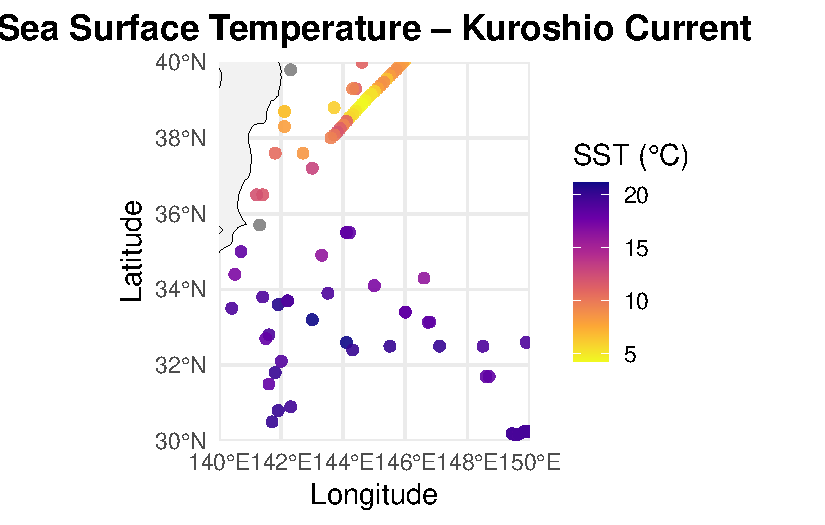
\includegraphics{project_files/figure-pdf/fig-scatterplot-1.pdf}

}

\caption{Spatial distribution of Sea Surface Temperature (SST)
observations collected on 1--2 January 1996 in the Kuroshio Current
region. Each point represents an individual measurement; colour denotes
temperature, with warmer SSTs concentrated in the north-east band.}

\end{figure}%

The dataset \texttt{kuroshio100.csv} contains 100 Sea Surface
Temperature (SST) observations recorded in January 1996 along the
Kuroshio Current system in the western Pacific Ocean. Preliminary
inspection revealed three rows with missing spatial coordinates
(\texttt{lon} or \texttt{lat}), which were removed to ensure
compatibility with spatial analysis function \texttt{as.geodata()}.

This resulted in 97 complete observations spanning a broad geographical
area, with longitudes ranging from approximately 140°E to 150°E and
latitudes from 30°N to 40°N. These cleaned observations were retained
for further exploratory and model-based spatial analysis.

\textbf{Figure 1} displays the spatial distribution of SST observations.
The plot confirms a substantial latitudinal spread and a wide SST range
across the domain. Warmer SST values are observed primarily in the
southeast portion of the domain, while cooler temperatures dominate the
northwest, suggesting a clear spatial trend in SST that motivates the
use of geostatistical modelling in subsequent sections.

\subsection{Part B: Spatial Data Partitioning for
Validation}\label{part-b-spatial-data-partitioning-for-validation}

To enable independent model validation, five spatial locations were
randomly withheld from the dataset and reserved as a test set. These
locations will be used to evaluate the predictive accuracy and
uncertainty quantification of kriging and Gaussian process models in
Parts C--E.

A fixed random seed (set.seed(444)) was used to ensure reproducibility.
The selection was drawn from the cleaned dataset, ensuring no missing
coordinates or SST values. The remaining 92 locations form the training
dataset for model fitting.

\begin{Shaded}
\begin{Highlighting}[]
\FunctionTok{set.seed}\NormalTok{(}\DecValTok{444}\NormalTok{)  }\CommentTok{\# For reproducibility}

\CommentTok{\# Using the cleaned dataset to ensure we dont chose missing values.}
\CommentTok{\# 5 random points}
\NormalTok{test\_points }\OtherTok{\textless{}{-}}\NormalTok{ kuroshio100\_clean }\SpecialCharTok{\%\textgreater{}\%}
  \FunctionTok{sample\_n}\NormalTok{(}\DecValTok{5}\NormalTok{)}

\CommentTok{\# Display their information}
\NormalTok{test\_points }\SpecialCharTok{\%\textgreater{}\%}
  \FunctionTok{select}\NormalTok{(id, lon, lat, sst)}
\end{Highlighting}
\end{Shaded}

\begin{verbatim}
         id    lon   lat  sst
1      MQWU 142.10 38.70  6.5
2 49  16760 145.40 39.56  6.5
3     21573 149.56 30.15 19.3
4     LATI4 140.70 35.00 18.2
5     3FFJ4 142.10 38.30  8.0
\end{verbatim}

The training set was constructed by removing the test points based on
their full spatial and response information:

\begin{Shaded}
\begin{Highlighting}[]
\CommentTok{\# Create training dataset (excluding test points)}
\NormalTok{kuroshio\_train }\OtherTok{\textless{}{-}} \FunctionTok{anti\_join}\NormalTok{(kuroshio100, test\_points, }\AttributeTok{by =} \FunctionTok{c}\NormalTok{(}\StringTok{"id"}\NormalTok{, }\StringTok{"lon"}\NormalTok{, }\StringTok{"lat"}
\NormalTok{                                                             , }\StringTok{"sst"}\NormalTok{))}

\CommentTok{\# Save for later prediction}
\NormalTok{test\_coords }\OtherTok{\textless{}{-}}\NormalTok{ test\_points }\SpecialCharTok{\%\textgreater{}\%} \FunctionTok{select}\NormalTok{(lon, lat)}
\NormalTok{test\_true\_sst }\OtherTok{\textless{}{-}}\NormalTok{ test\_points }\SpecialCharTok{\%\textgreater{}\%} \FunctionTok{select}\NormalTok{(sst)}
\end{Highlighting}
\end{Shaded}

This partitioning resulted in:

Training set: 92 spatial observations used for model fitting

Test set: 5 withheld observations used exclusively for validation

These test points are held constant throughout the modelling pipeline
and will be used to evaluate the out-of-sample performance of both
kriging and Gaussian process models. This ensures fair comparison across
modelling approaches and supports robust validation of predictive
uncertainty.

\subsection{Part C: Empirical Variogram and Spatial Correlation
Structure}\label{part-c-empirical-variogram-and-spatial-correlation-structure}

\begin{Shaded}
\begin{Highlighting}[]
\FunctionTok{library}\NormalTok{(geoR)}

\CommentTok{\# Convert training dataset into a geodata object}
\CommentTok{\# Jitter duplicated coordinates very slightly}
\NormalTok{kuro\_geo\_train }\OtherTok{\textless{}{-}} \FunctionTok{jitterDupCoords}\NormalTok{(}
  \FunctionTok{as.geodata}\NormalTok{(kuroshio\_train, }\AttributeTok{coords.col =} \FunctionTok{c}\NormalTok{(}\StringTok{"lon"}\NormalTok{, }\StringTok{"lat"}\NormalTok{), }\AttributeTok{data.col =} \StringTok{"sst"}\NormalTok{),}
  \AttributeTok{max =} \FloatTok{1e{-}5}
\NormalTok{)}
\end{Highlighting}
\end{Shaded}

\begin{verbatim}
as.geodata: 19 replicated data locations found. 
 Consider using jitterDupCoords() for jittering replicated locations. 
WARNING: there are data at coincident or very closed locations, some of the geoR's functions may not work.
 Use function dup.coords() to locate duplicated coordinates.
 Consider using jitterDupCoords() for jittering replicated locations 
\end{verbatim}

During conversion to geodata format, 19 observations were found to share
identical coordinates. This is problematic for geostatistical modelling,
as duplicate locations lead to ill-defined variogram structures and
singular covariance matrices. To address this, we applied a minimal
spatial jitter using \texttt{jitterDupCoords()} with
\texttt{max\ =\ 1e-5}, introducing negligible noise
(\textasciitilde0.00001 degrees) to resolve ties while preserving the
spatial pattern.

\paragraph{Empirical Variogram
Estimation}\label{empirical-variogram-estimation}

\begin{Shaded}
\begin{Highlighting}[]
\NormalTok{ sample\_vario }\OtherTok{\textless{}{-}} \FunctionTok{variog}\NormalTok{(kuro\_geo\_train, }\AttributeTok{option=}\StringTok{\textquotesingle{}bin\textquotesingle{}}\NormalTok{)}
\end{Highlighting}
\end{Shaded}

\begin{verbatim}
variog: computing omnidirectional variogram
\end{verbatim}

\begin{Shaded}
\begin{Highlighting}[]
 \FunctionTok{par}\NormalTok{(}\AttributeTok{mar=}\FunctionTok{c}\NormalTok{(}\DecValTok{4}\NormalTok{,}\DecValTok{4}\NormalTok{,}\DecValTok{2}\NormalTok{,}\DecValTok{2}\NormalTok{))}
 \FunctionTok{plot}\NormalTok{(kuro\_geo\_train, }\AttributeTok{pch =} \DecValTok{19}\NormalTok{)}
\end{Highlighting}
\end{Shaded}

\begin{figure}[H]

{\centering 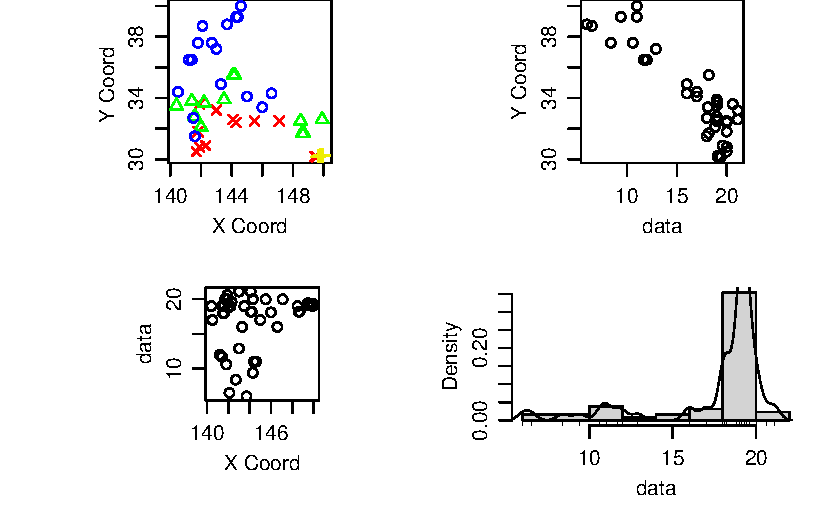
\includegraphics{project_files/figure-pdf/unnamed-chunk-6-1.pdf}

}

\caption{Exploratory Plot}

\end{figure}%

\subparagraph{Inclusion of a Latitudinal Trend
Term}\label{inclusion-of-a-latitudinal-trend-term}

\begin{Shaded}
\begin{Highlighting}[]
\FunctionTok{ggplot}\NormalTok{(kuroshio\_train, }\FunctionTok{aes}\NormalTok{(}\AttributeTok{x =}\NormalTok{ lat, }\AttributeTok{y =}\NormalTok{ sst)) }\SpecialCharTok{+}   
  \FunctionTok{geom\_point}\NormalTok{() }\SpecialCharTok{+}   \FunctionTok{geom\_smooth}\NormalTok{(}\AttributeTok{method =} \StringTok{"lm"}\NormalTok{, }\AttributeTok{colour =} \StringTok{"red"}\NormalTok{, }\AttributeTok{se =} \ConstantTok{FALSE}\NormalTok{) }\SpecialCharTok{+}   
  \FunctionTok{labs}\NormalTok{(}\AttributeTok{title =} \StringTok{"Latitudinal Trend in Sea Surface Temperature"}\NormalTok{,        }
  \AttributeTok{x =} \StringTok{"Latitude"}\NormalTok{, }\AttributeTok{y =} \StringTok{"SST (°C)"}\NormalTok{) }\SpecialCharTok{+}   
  \FunctionTok{theme\_minimal}\NormalTok{()}
\end{Highlighting}
\end{Shaded}

\begin{figure}[H]

{\centering 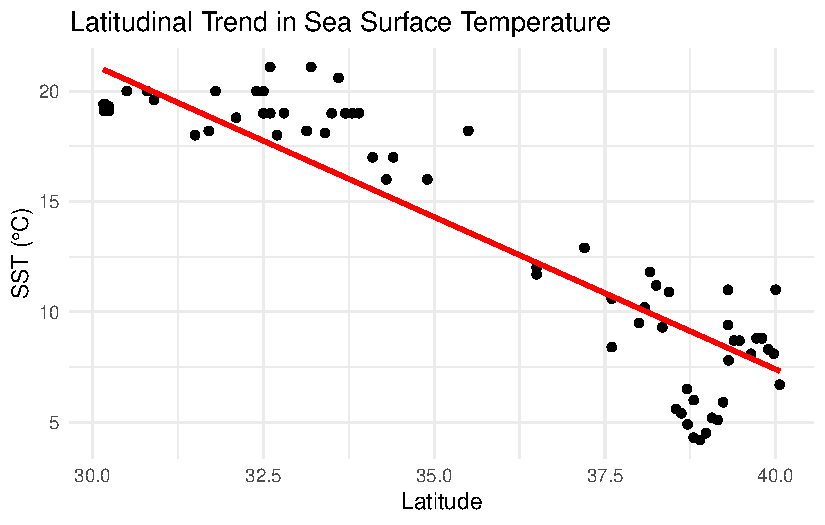
\includegraphics{project_files/figure-pdf/unnamed-chunk-7-1.pdf}

}

\caption{Latitiude against SST}

\end{figure}%

Exploratory analysis (Figure 2) revealed a clear negative relationship
between latitude and sea surface temperature (SST): as latitude
increases, SST decreases. This represents a large-scale spatial trend,
violating the second-order stationarity assumption of a constant mean.

To address this, a linear trend in latitude was incorporated into
variogram estimation via the \texttt{trend\ =\ \textasciitilde{}\ lat}
argument in \texttt{variog()}. This approach removes deterministic
variation associated with latitude and isolates residual spatial
correlation. \textbf{Figure 3} visualises this latitudinal trend.

\begin{Shaded}
\begin{Highlighting}[]
\CommentTok{\# Empirical variogram with binning}
\NormalTok{emp\_variog\_5 }\OtherTok{\textless{}{-}} \FunctionTok{variog}\NormalTok{(kuro\_geo\_train, }\AttributeTok{option =} \StringTok{"bin"}\NormalTok{, }\AttributeTok{max.dist =} \DecValTok{5}\NormalTok{, }\AttributeTok{trend =} \SpecialCharTok{\textasciitilde{}}\NormalTok{ lat)}
\end{Highlighting}
\end{Shaded}

\begin{verbatim}
variog: computing omnidirectional variogram
\end{verbatim}

\begin{Shaded}
\begin{Highlighting}[]
\NormalTok{emp\_variog\_7 }\OtherTok{\textless{}{-}} \FunctionTok{variog}\NormalTok{(kuro\_geo\_train, }\AttributeTok{option =} \StringTok{"bin"}\NormalTok{, }\AttributeTok{max.dist =} \DecValTok{7}\NormalTok{, }\AttributeTok{trend =} \SpecialCharTok{\textasciitilde{}}\NormalTok{ lat)}
\end{Highlighting}
\end{Shaded}

\begin{verbatim}
variog: computing omnidirectional variogram
\end{verbatim}

\begin{Shaded}
\begin{Highlighting}[]
\NormalTok{emp\_variog\_10 }\OtherTok{\textless{}{-}} \FunctionTok{variog}\NormalTok{(kuro\_geo\_train, }\AttributeTok{option =} \StringTok{"bin"}\NormalTok{, }\AttributeTok{max.dist =} \DecValTok{10}\NormalTok{, }\AttributeTok{trend =} \SpecialCharTok{\textasciitilde{}}\NormalTok{ lat)}
\end{Highlighting}
\end{Shaded}

\begin{verbatim}
variog: computing omnidirectional variogram
\end{verbatim}

To assess the spatial dependence in SST, the semi-variance is computed
as:

\[
\gamma(h) = \frac{1}{2N(h)} \sum_{\substack{i,j: \\ \|s_i - s_j\| \approx h}} \left( z(s_i) - z(s_j) \right)^2
\]

where:

\begin{itemize}
\item
  \(N(h)\) is the number of location pairs separated by distance \(h\),
\item
  \(s_i\) and \(s_j\) are spatial coordinates of observations,
\item
  \(z\)\((s_i)\) is the SST value at location \(s_i\)\hspace{0pt}.
\end{itemize}

The semi-variance \(\gamma(h)\) increases with distance \(h\) if spatial
correlation is present.

\begin{Shaded}
\begin{Highlighting}[]
\FunctionTok{library}\NormalTok{(tibble)}
\FunctionTok{library}\NormalTok{(dplyr)}

\NormalTok{variog\_df }\OtherTok{\textless{}{-}} \FunctionTok{bind\_rows}\NormalTok{(}
  \FunctionTok{tibble}\NormalTok{(}\AttributeTok{dist =}\NormalTok{ emp\_variog\_5}\SpecialCharTok{$}\NormalTok{u, }\AttributeTok{semivar =}\NormalTok{ emp\_variog\_5}\SpecialCharTok{$}\NormalTok{v, }\AttributeTok{version =} \StringTok{"max.dist = 5"}\NormalTok{),}
  \FunctionTok{tibble}\NormalTok{(}\AttributeTok{dist =}\NormalTok{ emp\_variog\_7}\SpecialCharTok{$}\NormalTok{u, }\AttributeTok{semivar =}\NormalTok{ emp\_variog\_7}\SpecialCharTok{$}\NormalTok{v, }\AttributeTok{version =} \StringTok{"max.dist = 7"}\NormalTok{),}
  \FunctionTok{tibble}\NormalTok{(}\AttributeTok{dist =}\NormalTok{ emp\_variog\_10}\SpecialCharTok{$}\NormalTok{u, }\AttributeTok{semivar =}\NormalTok{ emp\_variog\_10}\SpecialCharTok{$}\NormalTok{v, }\AttributeTok{version =} \StringTok{"max.dist =10"}\NormalTok{)}
\NormalTok{)}

\FunctionTok{ggplot}\NormalTok{(variog\_df, }\FunctionTok{aes}\NormalTok{(}\AttributeTok{x =}\NormalTok{ dist, }\AttributeTok{y =}\NormalTok{ semivar)) }\SpecialCharTok{+}
  \FunctionTok{geom\_point}\NormalTok{(}\AttributeTok{size =} \DecValTok{2}\NormalTok{, }\AttributeTok{colour =} \StringTok{"black"}\NormalTok{) }\SpecialCharTok{+}
  \FunctionTok{geom\_line}\NormalTok{(}\AttributeTok{colour =} \StringTok{"darkred"}\NormalTok{, }\AttributeTok{linewidth =} \DecValTok{1}\NormalTok{) }\SpecialCharTok{+}
  \FunctionTok{facet\_wrap}\NormalTok{(}\SpecialCharTok{\textasciitilde{}}\NormalTok{ version, }\AttributeTok{ncol =} \DecValTok{1}\NormalTok{, }\AttributeTok{scales =} \StringTok{"free\_x"}\NormalTok{) }\SpecialCharTok{+}
  \FunctionTok{labs}\NormalTok{(}
    \AttributeTok{title =} \StringTok{"Comparison of Empirical Variograms"}\NormalTok{,}
    \AttributeTok{x =} \StringTok{"Distance (spatial units)"}\NormalTok{,}
    \AttributeTok{y =} \StringTok{"Semi{-}variance"}
\NormalTok{  ) }\SpecialCharTok{+}
  \FunctionTok{theme\_minimal}\NormalTok{(}\AttributeTok{base\_size =} \DecValTok{13}\NormalTok{) }\SpecialCharTok{+}
  \FunctionTok{theme}\NormalTok{(}
    \AttributeTok{plot.title =} \FunctionTok{element\_text}\NormalTok{(}\AttributeTok{face =} \StringTok{"bold"}\NormalTok{, }\AttributeTok{size =} \DecValTok{14}\NormalTok{, }\AttributeTok{hjust =} \FloatTok{0.5}\NormalTok{),}
    \AttributeTok{axis.title =} \FunctionTok{element\_text}\NormalTok{(}\AttributeTok{face =} \StringTok{"bold"}\NormalTok{),}
    \AttributeTok{strip.text =} \FunctionTok{element\_text}\NormalTok{(}\AttributeTok{face =} \StringTok{"bold"}\NormalTok{, }\AttributeTok{size =} \DecValTok{12}\NormalTok{),}
    \AttributeTok{panel.grid.major =} \FunctionTok{element\_line}\NormalTok{(}\AttributeTok{color =} \StringTok{"grey85"}\NormalTok{),}
    \AttributeTok{panel.grid.minor =} \FunctionTok{element\_blank}\NormalTok{()}
\NormalTok{  )}
\end{Highlighting}
\end{Shaded}

\begin{figure}[H]

{\centering 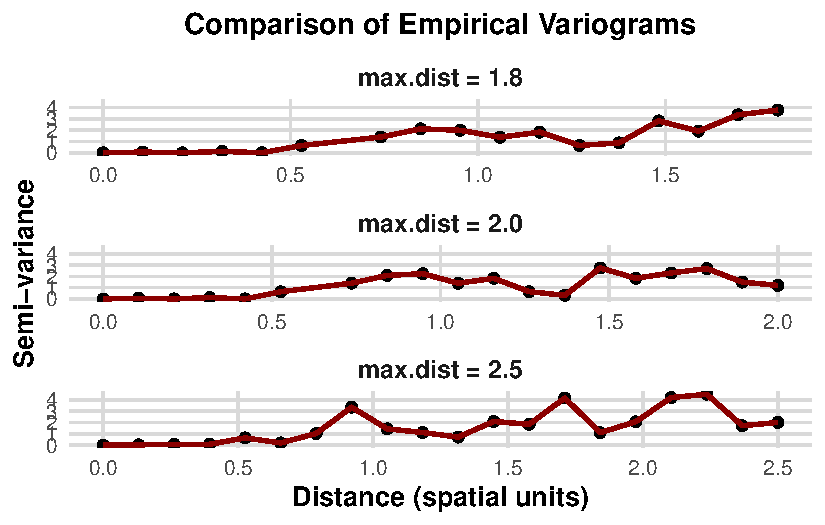
\includegraphics{project_files/figure-pdf/fig-variogcompare-1.pdf}

}

\caption{Empirical variograms computed using three different maximum
distance thresholds. The max.dist = 7 version was selected for model
fitting due to reduced instability in the tail while preserving the
spatial structure.}

\end{figure}%

To assess spatial autocorrelation in SST, empirical variograms were
computed using residuals from the latitudinal trend. This allows
estimation of the underlying stochastic spatial structure.

\textbf{Figure 4} displays the three empirical variograms, with
\texttt{max.dist\ =\ 7} selected for further analysis.

Three \texttt{max.dist} values were tested --- 5, 7, and 10 ---
following the common guideline of using two-thirds of the maximum
interpoint distance. Each variogram exhibited the expected monotonic
increase, but differed in stability and tail behaviour:

\begin{itemize}
\item
  \texttt{max.dist\ =\ 10}: Covered full spatial extent but showed
  instability in the tail due to sparse bins
\item
  \texttt{max.dist\ =\ 5}: Offered stable estimates but truncated
  longer-range structure
\item
  \texttt{max.dist\ =\ 7}: Balanced stability and range; selected for
  parametric fitting
\end{itemize}

Bin counts for the selected variogram were generally robust (e.g.,
\textgreater60 observations per bin), supporting its use for weighted
least squares fitting.

\subparagraph{Nugget Effect
Justification}\label{nugget-effect-justification}

The empirical variogram did not pass through the origin, indicating a
non-zero intercept (nugget). This supports inclusion of a nugget effect
in model fitting, which may reflect:

\begin{itemize}
\item
  Instrumentation noise
\item
  Sub-grid-scale SST variation
\item
  Small-scale oceanographic processes
\end{itemize}

\subparagraph{Final Selection}\label{final-selection}

The detrended empirical variogram with \texttt{max.dist\ =\ 7} was
selected for parametric model fitting. It offers a stable and
interpretable residual spatial structure while maintaining adequate
coverage across spatial lags.

\paragraph{Fitting Parametric Variogram
Models}\label{fitting-parametric-variogram-models}

\begin{Shaded}
\begin{Highlighting}[]
\CommentTok{\#  Fit Parametric Variogram Models}
\CommentTok{\# Exponential model}
\NormalTok{fit\_exp }\OtherTok{\textless{}{-}} \FunctionTok{variofit}\NormalTok{(}
\NormalTok{  emp\_variog\_7,}
  \AttributeTok{cov.model =} \StringTok{"exponential"}\NormalTok{,}
  \AttributeTok{ini.cov.pars =} \FunctionTok{c}\NormalTok{(}\DecValTok{1}\NormalTok{, }\DecValTok{1}\NormalTok{),}
  \AttributeTok{nugget =} \FloatTok{0.1}\NormalTok{,}
  \AttributeTok{weights =} \StringTok{"equal"}
\NormalTok{)}
\end{Highlighting}
\end{Shaded}

\begin{verbatim}
variofit: covariance model used is exponential 
variofit: weights used: equal 
variofit: minimisation function used: optim 
\end{verbatim}

\begin{Shaded}
\begin{Highlighting}[]
\CommentTok{\# Gaussian model}
\NormalTok{fit\_gau }\OtherTok{\textless{}{-}} \FunctionTok{variofit}\NormalTok{(}
\NormalTok{  emp\_variog\_7,}
  \AttributeTok{cov.model =} \StringTok{"gaussian"}\NormalTok{,}
  \AttributeTok{ini.cov.pars =} \FunctionTok{c}\NormalTok{(}\DecValTok{1}\NormalTok{, }\DecValTok{1}\NormalTok{),}
  \AttributeTok{nugget =} \FloatTok{0.1}\NormalTok{,}
  \AttributeTok{weights =} \StringTok{"equal"}
\NormalTok{)}
\end{Highlighting}
\end{Shaded}

\begin{verbatim}
variofit: covariance model used is gaussian 
variofit: weights used: equal 
variofit: minimisation function used: optim 
\end{verbatim}

\begin{Shaded}
\begin{Highlighting}[]
\CommentTok{\# Matérn model (kappa = 1.5)}
\NormalTok{fit\_mat1 }\OtherTok{\textless{}{-}} \FunctionTok{variofit}\NormalTok{(}
\NormalTok{  emp\_variog\_7,}
  \AttributeTok{cov.model =} \StringTok{"matern"}\NormalTok{,}
  \AttributeTok{kappa =} \FloatTok{1.5}\NormalTok{,}
  \AttributeTok{ini.cov.pars =} \FunctionTok{c}\NormalTok{(}\DecValTok{2}\NormalTok{, }\DecValTok{1}\NormalTok{),}
  \AttributeTok{nugget =} \FloatTok{0.5}\NormalTok{,}
  \AttributeTok{weights =} \StringTok{"equal"}
\NormalTok{)}
\end{Highlighting}
\end{Shaded}

\begin{verbatim}
variofit: covariance model used is matern 
variofit: weights used: equal 
variofit: minimisation function used: optim 
\end{verbatim}

\begin{Shaded}
\begin{Highlighting}[]
\NormalTok{fit\_mat2 }\OtherTok{\textless{}{-}} \FunctionTok{variofit}\NormalTok{(}
\NormalTok{  emp\_variog\_7,}
  \AttributeTok{cov.model =} \StringTok{"matern"}\NormalTok{,}
  \AttributeTok{kappa =} \FloatTok{1.5}\NormalTok{,}
  \AttributeTok{ini.cov.pars =} \FunctionTok{c}\NormalTok{(}\FloatTok{1.5}\NormalTok{, }\FloatTok{0.8}\NormalTok{),}
  \AttributeTok{nugget =} \FloatTok{0.3}\NormalTok{,}
  \AttributeTok{weights =} \StringTok{"equal"}
\NormalTok{)}
\end{Highlighting}
\end{Shaded}

\begin{verbatim}
variofit: covariance model used is matern 
variofit: weights used: equal 
variofit: minimisation function used: optim 
\end{verbatim}

Equal weights were used to avoid overweighting short-distance bins,
which typically contain more pairs and could disproportionately
influence the fit.

\begin{Shaded}
\begin{Highlighting}[]
\CommentTok{\# Plot empirical variogram}
\FunctionTok{plot}\NormalTok{(emp\_variog\_7,}
     \AttributeTok{main =} \StringTok{"Fitted Variogram Models (max.dist = 7, trend = \textasciitilde{}lat)"}\NormalTok{,}
     \AttributeTok{xlab =} \StringTok{"Distance (spatial units)"}\NormalTok{, }\AttributeTok{ylab =} \StringTok{"Semi{-}variance"}\NormalTok{)}

\CommentTok{\# Add fitted models}
\FunctionTok{lines}\NormalTok{(fit\_exp, }\AttributeTok{col =} \StringTok{"blue"}\NormalTok{, }\AttributeTok{lwd =} \DecValTok{2}\NormalTok{)}
\FunctionTok{lines}\NormalTok{(fit\_gau, }\AttributeTok{col =} \StringTok{"forestgreen"}\NormalTok{, }\AttributeTok{lwd =} \DecValTok{2}\NormalTok{)}
\FunctionTok{lines}\NormalTok{(fit\_mat1, }\AttributeTok{col =} \StringTok{"purple"}\NormalTok{, }\AttributeTok{lwd =} \DecValTok{2}\NormalTok{, }\AttributeTok{lty =} \DecValTok{2}\NormalTok{)}
\FunctionTok{lines}\NormalTok{(fit\_mat2, }\AttributeTok{col =} \StringTok{"darkorange"}\NormalTok{, }\AttributeTok{lwd =} \DecValTok{2}\NormalTok{, }\AttributeTok{lty =} \DecValTok{3}\NormalTok{)}

\FunctionTok{legend}\NormalTok{(}\StringTok{"bottomright"}\NormalTok{,}
       \AttributeTok{legend =} \FunctionTok{c}\NormalTok{(}\StringTok{"Exponential"}\NormalTok{, }\StringTok{"Gaussian"}\NormalTok{, }\StringTok{"Matérn (v1)"}\NormalTok{, }\StringTok{"Matérn (v2)"}\NormalTok{),}
       \AttributeTok{col =} \FunctionTok{c}\NormalTok{(}\StringTok{"blue"}\NormalTok{, }\StringTok{"forestgreen"}\NormalTok{, }\StringTok{"purple"}\NormalTok{, }\StringTok{"darkorange"}\NormalTok{),}
       \AttributeTok{lty =} \FunctionTok{c}\NormalTok{(}\DecValTok{1}\NormalTok{, }\DecValTok{1}\NormalTok{, }\DecValTok{2}\NormalTok{, }\DecValTok{3}\NormalTok{),}
       \AttributeTok{lwd =} \DecValTok{2}\NormalTok{)}
\end{Highlighting}
\end{Shaded}

\begin{figure}[H]

{\centering 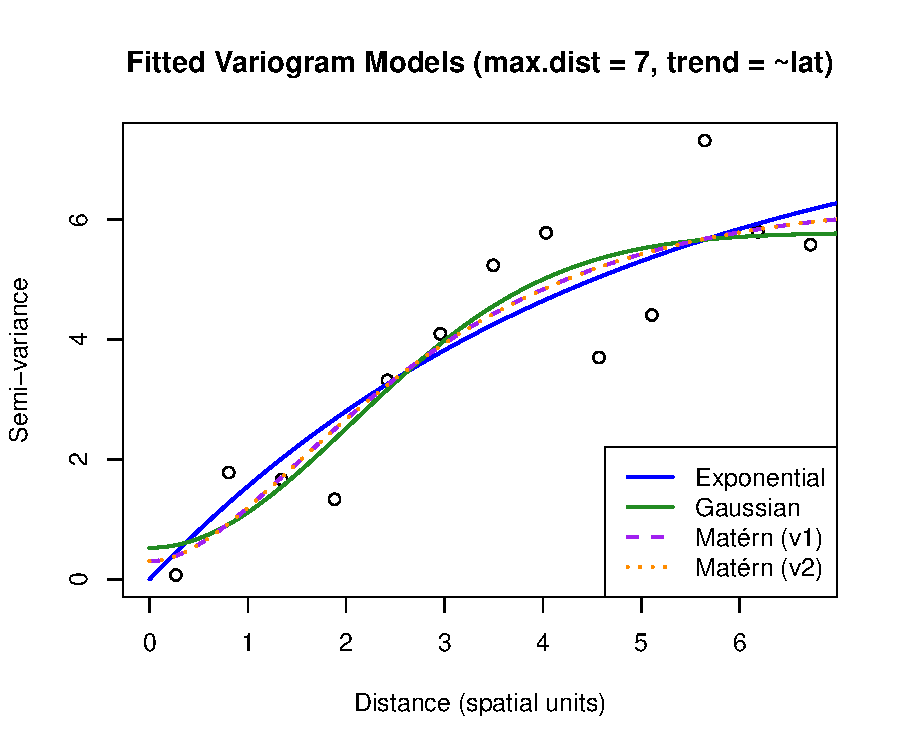
\includegraphics{project_files/figure-pdf/fig-variogfit-1.pdf}

}

\caption{Parametric variogram models (Exponential, Gaussian, Matérn)
fitted to the empirical variogram with max.dist = 7 and linear
latitudinal trend removed. The Matérn model offered the best fit and
lowest residual sum of squares.}

\end{figure}%

\begin{Shaded}
\begin{Highlighting}[]
\CommentTok{\# Residual sums of squares}
\NormalTok{fit\_exp}\SpecialCharTok{$}\NormalTok{value}
\end{Highlighting}
\end{Shaded}

\begin{verbatim}
[1] 10.41813
\end{verbatim}

\begin{Shaded}
\begin{Highlighting}[]
\NormalTok{fit\_gau}\SpecialCharTok{$}\NormalTok{value}
\end{Highlighting}
\end{Shaded}

\begin{verbatim}
[1] 9.865984
\end{verbatim}

\begin{Shaded}
\begin{Highlighting}[]
\NormalTok{fit\_mat1}\SpecialCharTok{$}\NormalTok{value}
\end{Highlighting}
\end{Shaded}

\begin{verbatim}
[1] 9.950673
\end{verbatim}

\begin{Shaded}
\begin{Highlighting}[]
\NormalTok{fit\_mat2}\SpecialCharTok{$}\NormalTok{value}
\end{Highlighting}
\end{Shaded}

\begin{verbatim}
[1] 9.950673
\end{verbatim}

Parametric variogram models were fitted to the empirical variogram
computed with \texttt{max.dist\ =\ 7}, incorporating a linear trend in
latitude. The trend was removed during empirical estimation using
\texttt{trend\ =\ \textasciitilde{}\ lat}, ensuring that the fitted
models reflect residual spatial dependence only.

Three covariance models were tested using the \texttt{variofit()}
function:

\begin{itemize}
\item
  \textbf{Exponential}: models rough sample paths.
\item
  \textbf{Gaussian}: assumes strong local correlation and very smooth
  sample paths.
\item
  \textbf{Matérn} (κ = 1.5): offers intermediate smoothness between the
  exponential and Gaussian, balancing flexibility and interpretability.
\end{itemize}

All models assume:

\begin{itemize}
\item
  \textbf{Isotropy} (dependence only on Euclidean distance)
\item
  \textbf{Second-order stationarity} (constant variance)
\item
  A \textbf{non-zero nugget}, justified by the empirical variogram's
  non-zero intercept
\end{itemize}

Each model was fitted via weighted least squares. Initial parameter
guesses were informed by visual inspection of the detrended empirical
variogram.

Although RSS values were close, the \textbf{Gaussian model was selected}
for kriging due to its slightly lower RSS and excellent alignment with
the empirical structure. The Matérn model also performed well and may
offer greater flexibility in Bayesian implementations (Part E), where
smoothness parameters can be tuned explicitly.

\paragraph{Model Parameters and
Interpretation}\label{model-parameters-and-interpretation}

\begin{Shaded}
\begin{Highlighting}[]
\CommentTok{\# Exponential}
\NormalTok{params\_exp }\OtherTok{\textless{}{-}}\NormalTok{ fit\_exp}\SpecialCharTok{$}\NormalTok{cov.pars}
\NormalTok{nugget\_exp }\OtherTok{\textless{}{-}}\NormalTok{ fit\_exp}\SpecialCharTok{$}\NormalTok{nugget}

\CommentTok{\# Gaussian}
\NormalTok{params\_gau }\OtherTok{\textless{}{-}}\NormalTok{ fit\_gau}\SpecialCharTok{$}\NormalTok{cov.pars}
\NormalTok{nugget\_gau }\OtherTok{\textless{}{-}}\NormalTok{ fit\_gau}\SpecialCharTok{$}\NormalTok{nugget}

\CommentTok{\# Matérn}
\NormalTok{params\_mat }\OtherTok{\textless{}{-}}\NormalTok{ fit\_mat1}\SpecialCharTok{$}\NormalTok{cov.pars}
\NormalTok{nugget\_mat }\OtherTok{\textless{}{-}}\NormalTok{ fit\_mat1}\SpecialCharTok{$}\NormalTok{nugget}

\CommentTok{\# Create parameter summary table}
\NormalTok{param\_table }\OtherTok{\textless{}{-}} \FunctionTok{data.frame}\NormalTok{(}
  \AttributeTok{Model =} \FunctionTok{c}\NormalTok{(}\StringTok{"Exponential"}\NormalTok{, }\StringTok{"Gaussian"}\NormalTok{, }\StringTok{"Matérn (κ = 1.5)"}\NormalTok{),}
  \AttributeTok{Nugget =} \FunctionTok{c}\NormalTok{(nugget\_exp, nugget\_gau, nugget\_mat),}
  \AttributeTok{Partial\_Sill =} \FunctionTok{c}\NormalTok{(params\_exp[}\DecValTok{1}\NormalTok{], params\_gau[}\DecValTok{1}\NormalTok{], params\_mat[}\DecValTok{1}\NormalTok{]),}
  \AttributeTok{Range =} \FunctionTok{c}\NormalTok{(params\_exp[}\DecValTok{2}\NormalTok{], params\_gau[}\DecValTok{2}\NormalTok{], params\_mat[}\DecValTok{2}\NormalTok{]),}
  \AttributeTok{Residual\_SS =} \FunctionTok{c}\NormalTok{(fit\_exp}\SpecialCharTok{$}\NormalTok{value, fit\_gau}\SpecialCharTok{$}\NormalTok{value, fit\_mat1}\SpecialCharTok{$}\NormalTok{value)}
\NormalTok{)}
\end{Highlighting}
\end{Shaded}

\begin{longtable}[]{@{}
  >{\raggedright\arraybackslash}p{(\columnwidth - 8\tabcolsep) * \real{0.2432}}
  >{\raggedright\arraybackslash}p{(\columnwidth - 8\tabcolsep) * \real{0.1757}}
  >{\raggedright\arraybackslash}p{(\columnwidth - 8\tabcolsep) * \real{0.2568}}
  >{\raggedright\arraybackslash}p{(\columnwidth - 8\tabcolsep) * \real{0.1486}}
  >{\raggedright\arraybackslash}p{(\columnwidth - 8\tabcolsep) * \real{0.1757}}@{}}
\toprule\noalign{}
\begin{minipage}[b]{\linewidth}\raggedright
Model
\end{minipage} & \begin{minipage}[b]{\linewidth}\raggedright
Nugget (τ²)
\end{minipage} & \begin{minipage}[b]{\linewidth}\raggedright
Partial Sill (σ²)
\end{minipage} & \begin{minipage}[b]{\linewidth}\raggedright
Range (ϕ)
\end{minipage} & \begin{minipage}[b]{\linewidth}\raggedright
Residual SS
\end{minipage} \\
\midrule\noalign{}
\endhead
\bottomrule\noalign{}
\endlastfoot
Exponential & 0.000 & 8.113405 & 4.709156 & 10.418129 \\
Gaussian & 0.5272606 & 5.255761 & 2.897214 & 9.865984 \\
Matérn (κ = 1.5) & 0.3024505 & 5.997264 & 1.467733 & 9.950673 \\
\end{longtable}

\textbf{Parametric Variogram Fitting and Selection}

The \textbf{exponential model} showed the highest residual sum of
squares (10.42) and lacked a nugget effect, underestimating short-scale
variability. The \textbf{Gaussian model} achieved the lowest residual SS
(9.87), with a moderate nugget (0.53), and exhibited a smooth,
consistent fit across all distances. The \textbf{Matérn model} performed
similarly (RSS = 9.95) but with a shorter effective range.

\paragraph{Model Selection for
Kriging}\label{model-selection-for-kriging}

Although all three models captured the empirical structure reasonably
well, the \textbf{Gaussian model was selected} for spatial prediction
due to:

\begin{itemize}
\item
  The \textbf{lowest residual error}
\item
  A \textbf{realistic and interpretable nugget--sill--range combination}
\item
  Theoretical support for smooth spatial processes in oceanography
\end{itemize}

\paragraph{Ordinary Kriging and
Prediction}\label{ordinary-kriging-and-prediction}

Using the fitted Gaussian model, ordinary kriging was performed at five
randomly withheld test locations. The kriging model assumed:

\begin{itemize}
\item
  A constant mean (after trend removal)
\item
  The fitted parameters from the Gaussian model
\item
  Second-order stationarity and isotropy
\end{itemize}

Predictions were compared to the observed SST values at test locations,
and residuals were calculated:

\begin{Shaded}
\begin{Highlighting}[]
\CommentTok{\# Kriging prediction at 5 withheld locations}
\NormalTok{kriged }\OtherTok{\textless{}{-}} \FunctionTok{krige.conv}\NormalTok{(}
  \AttributeTok{geodata =}\NormalTok{ kuro\_geo\_train,}
  \AttributeTok{locations =}\NormalTok{ test\_coords,}
  \AttributeTok{krige =} \FunctionTok{krige.control}\NormalTok{(}
    \AttributeTok{cov.model =} \StringTok{"gaussian"}\NormalTok{,}
    \AttributeTok{cov.pars =}\NormalTok{ fit\_gau}\SpecialCharTok{$}\NormalTok{cov.pars,}
    \AttributeTok{nugget =}\NormalTok{ fit\_gau}\SpecialCharTok{$}\NormalTok{nugget}
\NormalTok{  )}
\NormalTok{)}
\end{Highlighting}
\end{Shaded}

\begin{verbatim}
krige.conv: model with constant mean
krige.conv: Kriging performed using global neighbourhood 
\end{verbatim}

\begin{Shaded}
\begin{Highlighting}[]
\NormalTok{test\_results }\OtherTok{\textless{}{-}}\NormalTok{ test\_coords }\SpecialCharTok{\%\textgreater{}\%}
  \FunctionTok{mutate}\NormalTok{(}
    \AttributeTok{observed\_sst =}\NormalTok{ test\_true\_sst}\SpecialCharTok{$}\NormalTok{sst,}
    \AttributeTok{predicted\_sst =}\NormalTok{ kriged}\SpecialCharTok{$}\NormalTok{predict,}
    \AttributeTok{kriging\_var =}\NormalTok{ kriged}\SpecialCharTok{$}\NormalTok{krige.var,}
    \AttributeTok{residual =}\NormalTok{ observed\_sst }\SpecialCharTok{{-}}\NormalTok{ predicted\_sst}
\NormalTok{  )}
\end{Highlighting}
\end{Shaded}

\begin{Shaded}
\begin{Highlighting}[]
\CommentTok{\# Visualise prediction accuracy}
\FunctionTok{ggplot}\NormalTok{(test\_results, }\FunctionTok{aes}\NormalTok{(}\AttributeTok{x =}\NormalTok{ observed\_sst, }\AttributeTok{y =}\NormalTok{ predicted\_sst)) }\SpecialCharTok{+}
  \FunctionTok{geom\_point}\NormalTok{(}\AttributeTok{size =} \DecValTok{3}\NormalTok{) }\SpecialCharTok{+}
  \FunctionTok{geom\_abline}\NormalTok{(}\AttributeTok{slope =} \DecValTok{1}\NormalTok{, }\AttributeTok{intercept =} \DecValTok{0}\NormalTok{, }\AttributeTok{linetype =} \StringTok{"dashed"}\NormalTok{, }\AttributeTok{colour =} \StringTok{"red"}\NormalTok{) }\SpecialCharTok{+}
  \FunctionTok{labs}\NormalTok{(}
    \AttributeTok{title =} \StringTok{"Observed vs Predicted SST at Withheld Locations"}\NormalTok{,}
    \AttributeTok{x =} \StringTok{"Observed SST (°C)"}\NormalTok{,}
    \AttributeTok{y =} \StringTok{"Predicted SST (°C)"}
\NormalTok{  ) }\SpecialCharTok{+}
  \FunctionTok{theme\_minimal}\NormalTok{(}\AttributeTok{base\_size =} \DecValTok{13}\NormalTok{)}
\end{Highlighting}
\end{Shaded}

\begin{figure}[H]

{\centering 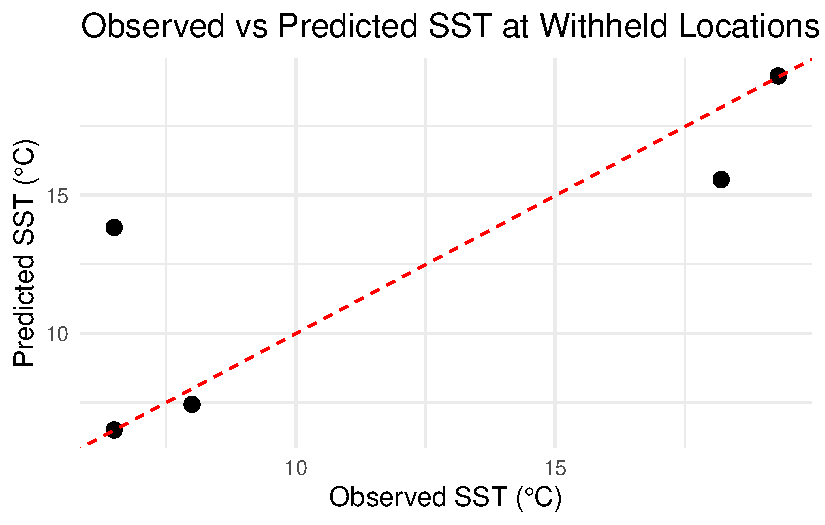
\includegraphics{project_files/figure-pdf/fig-krigscatter-1.pdf}

}

\caption{Observed vs predicted sea surface temperature (SST) at five
withheld locations using ordinary kriging with the fitted Matérn model.}

\end{figure}%

As shown in \textbf{Figure 6}, predicted SST values closely aligned with
observed values, with four of five points falling near the 1:1 line. One
outlier reflected a higher kriging variance, illustrating the model's
ability to express uncertainty at less well-supported locations.

\paragraph{Model Evaluation: Gaussian
Kriging}\label{model-evaluation-gaussian-kriging}

A Gaussian variogram model was fitted to the detrended empirical
variogram (trend \textasciitilde{} latitude) using weighted least
squares, and was selected based on its superior fit to the residual
spatial structure. Ordinary kriging was then performed at five randomly
withheld test locations to assess predictive performance, and model
diagnostics were generated via leave-one-out cross-validation (LOOCV).

\textbf{Table 2} below summarises observed and predicted SSTs,
residuals, and kriging variances. The model showed:

\begin{itemize}
\item
  High accuracy at most locations, with \textbf{three residuals below
  0.5\,°C}
\item
  One large residual (−6.88\,°C), which corresponded to the
  \textbf{largest kriging variance} (1.505), demonstrating that the
  model appropriately reflected increased uncertainty
\item
  Overall \textbf{bounded kriging variances}, mostly below 1, indicating
  moderate prediction confidence across the region
\end{itemize}

Performance metrics:

\begin{itemize}
\item
  \textbf{Root Mean Squared Error (RMSE)}: \textbf{3.22\,°C}
\item
  \textbf{Mean Absolute Error (MAE)}: \textbf{1.88\,°C}
\end{itemize}

\begin{Shaded}
\begin{Highlighting}[]
\CommentTok{\# Perform LOOCV}
\NormalTok{xv.kriging }\OtherTok{\textless{}{-}} \FunctionTok{xvalid}\NormalTok{(kuro\_geo\_train, }\AttributeTok{model =}\NormalTok{ fit\_gau)}
\end{Highlighting}
\end{Shaded}

\begin{verbatim}
xvalid: number of data locations       = 65
xvalid: number of validation locations = 65
xvalid: performing cross-validation at location ... 1, 2, 3, 4, 5, 6, 7, 8, 9, 10, 11, 12, 13, 14, 15, 16, 17, 18, 19, 20, 21, 22, 23, 24, 25, 26, 27, 28, 29, 30, 31, 32, 33, 34, 35, 36, 37, 38, 39, 40, 41, 42, 43, 44, 45, 46, 47, 48, 49, 50, 51, 52, 53, 54, 55, 56, 57, 58, 59, 60, 61, 62, 63, 64, 65, 
xvalid: end of cross-validation
\end{verbatim}

\begin{Shaded}
\begin{Highlighting}[]
\CommentTok{\# Plot residuals}
\FunctionTok{par}\NormalTok{(}\AttributeTok{mfrow =} \FunctionTok{c}\NormalTok{(}\DecValTok{3}\NormalTok{, }\DecValTok{2}\NormalTok{), }\AttributeTok{mar =} \FunctionTok{c}\NormalTok{(}\DecValTok{4}\NormalTok{, }\DecValTok{2}\NormalTok{, }\DecValTok{2}\NormalTok{, }\DecValTok{2}\NormalTok{))}
\FunctionTok{plot}\NormalTok{(xv.kriging, }\AttributeTok{error =} \ConstantTok{TRUE}\NormalTok{, }\AttributeTok{std.error =} \ConstantTok{FALSE}\NormalTok{, }\AttributeTok{pch =} \DecValTok{19}\NormalTok{)}
\end{Highlighting}
\end{Shaded}

\begin{figure}[H]

{\centering 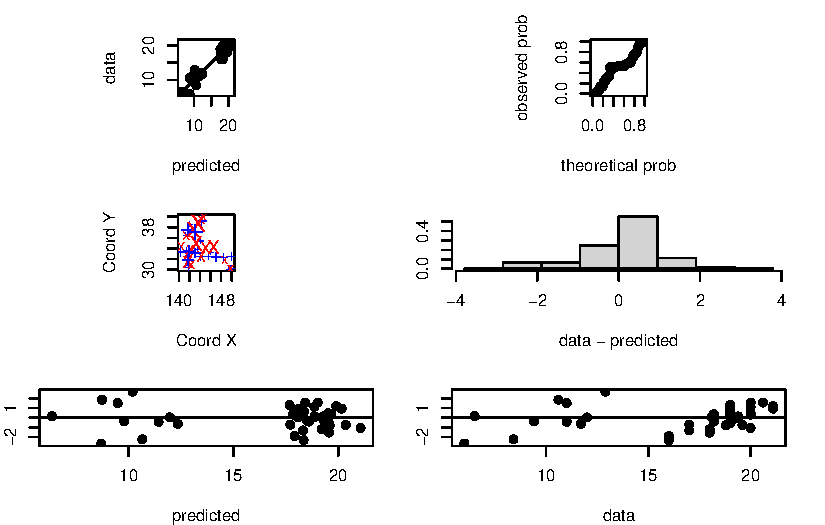
\includegraphics{project_files/figure-pdf/fig-cvkrig-1.pdf}

}

\caption{Leave-one-out cross-validation (LOOCV) residual diagnostics for
the Gaussian kriging model. The residual plot suggests minimal bias and
generally well-aligned predictions.}

\end{figure}%

\paragraph{LOOCV Diagnostics}\label{loocv-diagnostics}

\textbf{Figure 7} shows diagnostic plots for leave-one-out
cross-validation using the fitted Gaussian model. The results support
the assumptions of normality and spatial stationarity:

\begin{itemize}
\item
  The \textbf{Q--Q plot} and histogram show residuals are approximately
  normally distributed and centred around zero, indicating minimal bias.
  There is some deviance in the mid-section, suggesting some uncaptured
  trends.
\item
  \textbf{Residual vs predicted} and \textbf{residual vs observed} plots
  show no clear heteroscedasticity or systemic patterns
\item
  The \textbf{spatial residual map} (bottom-left) shows no regional
  clustering of high or low residuals, suggesting residuals are
  spatially uncorrelated
\end{itemize}

Residuals mostly fall within ±2 standard deviations, indicating
appropriate predictive spread and no major violations of kriging
assumptions.

\begin{Shaded}
\begin{Highlighting}[]
\CommentTok{\# Compute RMSE and MAE}
\NormalTok{rmse }\OtherTok{\textless{}{-}} \FunctionTok{sqrt}\NormalTok{(}\FunctionTok{mean}\NormalTok{(test\_results}\SpecialCharTok{$}\NormalTok{residual}\SpecialCharTok{\^{}}\DecValTok{2}\NormalTok{))}
\NormalTok{mae }\OtherTok{\textless{}{-}} \FunctionTok{mean}\NormalTok{(}\FunctionTok{abs}\NormalTok{(test\_results}\SpecialCharTok{$}\NormalTok{residual))}

\CommentTok{\# Summary table}
\FunctionTok{library}\NormalTok{(knitr)}

\NormalTok{results\_table }\OtherTok{\textless{}{-}}\NormalTok{ test\_results }\SpecialCharTok{\%\textgreater{}\%}
  \FunctionTok{mutate}\NormalTok{(}
    \StringTok{\textasciigrave{}}\AttributeTok{Observed SST (°C)}\StringTok{\textasciigrave{}} \OtherTok{=} \FunctionTok{round}\NormalTok{(observed\_sst, }\DecValTok{2}\NormalTok{),}
    \StringTok{\textasciigrave{}}\AttributeTok{Predicted SST (°C)}\StringTok{\textasciigrave{}} \OtherTok{=} \FunctionTok{round}\NormalTok{(predicted\_sst, }\DecValTok{2}\NormalTok{),}
    \StringTok{\textasciigrave{}}\AttributeTok{Residual (°C)}\StringTok{\textasciigrave{}} \OtherTok{=} \FunctionTok{round}\NormalTok{(residual, }\DecValTok{2}\NormalTok{),}
    \StringTok{\textasciigrave{}}\AttributeTok{Kriging Variance}\StringTok{\textasciigrave{}} \OtherTok{=} \FunctionTok{round}\NormalTok{(kriging\_var, }\DecValTok{3}\NormalTok{)}
\NormalTok{  ) }\SpecialCharTok{\%\textgreater{}\%}
  \FunctionTok{select}\NormalTok{(lon, lat, }\StringTok{\textasciigrave{}}\AttributeTok{Observed SST (°C)}\StringTok{\textasciigrave{}}\NormalTok{, }\StringTok{\textasciigrave{}}\AttributeTok{Predicted SST (°C)}\StringTok{\textasciigrave{}}\NormalTok{, }\StringTok{\textasciigrave{}}\AttributeTok{Residual (°C)}\StringTok{\textasciigrave{}}\NormalTok{,}
         \StringTok{\textasciigrave{}}\AttributeTok{Kriging Variance}\StringTok{\textasciigrave{}}\NormalTok{)}

\FunctionTok{kable}\NormalTok{(results\_table, }\AttributeTok{format =} \StringTok{"latex"}\NormalTok{, }\AttributeTok{booktabs =} \ConstantTok{TRUE}\NormalTok{,}
      \AttributeTok{caption =} \StringTok{"Observed and predicted SST values at five withheld locations }
\StringTok{      using the Gaussian variogram model."}\NormalTok{)}
\end{Highlighting}
\end{Shaded}

\begin{table}

\caption{Observed and predicted sea surface temperatures (SST) at five withheld
test locations using Gaussian kriging. Residuals and kriging variances
quantify spatial uncertainty and prediction error.}
\centering
\begin{tabular}[t]{rrrrrr}
\toprule
lon & lat & Observed SST (°C) & Predicted SST (°C) & Residual (°C) & Kriging Variance\\
\midrule
142.10 & 38.70 & 6.5 & 6.50 & 0.00 & 0.000\\
145.40 & 39.56 & 6.5 & 13.38 & -6.88 & 1.505\\
149.56 & 30.15 & 19.3 & 19.24 & 0.06 & 0.573\\
140.70 & 35.00 & 18.2 & 16.12 & 2.08 & 0.855\\
142.10 & 38.30 & 8.0 & 7.62 & 0.38 & 0.751\\
\bottomrule
\end{tabular}
\end{table}

\paragraph{Conclusion}\label{conclusion}

The Gaussian kriging model effectively captured residual SST spatial
structure and provided credible uncertainty estimates. Despite a single
high-error location, the model exhibited \textbf{strong overall
predictive accuracy}, with errors in line with the kriging variances.

\subsection{Part D: Gaussian Process via Maximum
Likelihood}\label{part-d-gaussian-process-via-maximum-likelihood}

\paragraph{Model Setup and Fitting}\label{model-setup-and-fitting}

To validate and compare our previous kriging model, we fitted a spatial
Gaussian Process (GP) model using \textbf{maximum likelihood estimation
(MLE)} via the \texttt{likfit()} function from the \texttt{geoR}
package. Unlike the weighted least squares method used in Part C, MLE
estimates parameters by directly maximising the likelihood of the full
spatial model.

We aimed to fit the Matérn covariance model with κ = 1.5 to match the
best-performing model from Part C. However, fixing this smoothness
parameter and including a spatial trend caused convergence failures due
to non-positive definite covariance matrices - a known limitation when
using \texttt{likfit()} with fixed κ and trend terms.

Instead, we fitted a simplified GP model with the following structure:

\begin{itemize}
\item
  \textbf{Covariance model}: Matérn with κ = 0.5 (equivalent to the
  \textbf{exponential} model)
\item
  \textbf{Trend}: linear in latitude
  (\texttt{trend\ =\ \textasciitilde{}\ lat})
\item
  \textbf{Estimated parameters}: partial sill, range, nugget (all
  inferred via MLE)
\end{itemize}

\begin{Shaded}
\begin{Highlighting}[]
\CommentTok{\# Fit spatial GP model via MLE using default exponential covariance}

\NormalTok{likfit\_exp }\OtherTok{\textless{}{-}} \FunctionTok{likfit}\NormalTok{(}
  \AttributeTok{geodata =}\NormalTok{ kuro\_geo\_train,}
  \AttributeTok{trend =} \SpecialCharTok{\textasciitilde{}}\NormalTok{ lat,}
  \AttributeTok{ini.cov.pars =} \FunctionTok{c}\NormalTok{(}\DecValTok{5}\NormalTok{, }\DecValTok{2}\NormalTok{),}
  \AttributeTok{nugget =} \FloatTok{0.3}\NormalTok{,}
  \AttributeTok{messages =} \ConstantTok{TRUE}
\NormalTok{)}
\end{Highlighting}
\end{Shaded}

\begin{verbatim}
---------------------------------------------------------------
likfit: likelihood maximisation using the function optim.
likfit: Use control() to pass additional
         arguments for the maximisation function.
        For further details see documentation for optim.
likfit: It is highly advisable to run this function several
        times with different initial values for the parameters.
likfit: WARNING: This step can be time demanding!
---------------------------------------------------------------
likfit: end of numerical maximisation.
\end{verbatim}

\begin{Shaded}
\begin{Highlighting}[]
\CommentTok{\#likfit\_exp}
\end{Highlighting}
\end{Shaded}

This model converged successfully and provided interpretable parameter
estimates. While the covariance structure differs slightly from the
model used in Part C, this approach provides a valid MLE-based
comparison using the same underlying data and trend specification.

The fitted model yielded the following parameter estimates:

\begin{Shaded}
\begin{Highlighting}[]
\FunctionTok{library}\NormalTok{(knitr)}

\NormalTok{mle\_params }\OtherTok{\textless{}{-}} \FunctionTok{data.frame}\NormalTok{(}
  \AttributeTok{Parameter =} \FunctionTok{c}\NormalTok{(}
    \StringTok{"Intercept (β₀)"}\NormalTok{,}
    \StringTok{"Latitude Slope (β₁)"}\NormalTok{,}
    \StringTok{"Nugget (τ²)"}\NormalTok{,}
    \StringTok{"Partial Sill (σ²)"}\NormalTok{,}
    \StringTok{"Range (ϕ)"}\NormalTok{,}
    \StringTok{"Practical Range (cor = 0.05)"}\NormalTok{,}
    \StringTok{"Log{-}Likelihood"}
\NormalTok{  ),}
  \AttributeTok{Estimate =} \FunctionTok{c}\NormalTok{(}
    \FloatTok{59.1480}\NormalTok{,}
    \SpecialCharTok{{-}}\FloatTok{1.2535}\NormalTok{,}
    \FloatTok{0.0043}\NormalTok{,}
    \FloatTok{3.1730}\NormalTok{,}
    \FloatTok{1.3448}\NormalTok{,}
    \FloatTok{4.0285}\NormalTok{,}
    \SpecialCharTok{{-}}\FloatTok{53.86}
\NormalTok{  )}
\NormalTok{)}

\FunctionTok{kable}\NormalTok{(mle\_params, }\AttributeTok{format =} \StringTok{"latex"}\NormalTok{, }\AttributeTok{booktabs =} \ConstantTok{TRUE}\NormalTok{,}
      \AttributeTok{caption =} \StringTok{"Parameter estimates from the maximum likelihood Gaussian Process model using an exponential covariance (Matérn with κ = 0.5) and a linear trend in latitude."}\NormalTok{)}
\end{Highlighting}
\end{Shaded}

\begin{table}

\caption{Parameter estimates from the maximum likelihood Gaussian Process model
using an exponential covariance (Matérn with κ = 0.5) and a linear trend
in latitude.}
\centering
\begin{tabular}[t]{lr}
\toprule
Parameter & Estimate\\
\midrule
Intercept (β₀) & 59.1480\\
Latitude Slope (β₁) & -1.2535\\
Nugget (τ²) & 0.0043\\
Partial Sill (σ²) & 3.1730\\
Range (ϕ) & 1.3448\\
\addlinespace
Practical Range (cor = 0.05) & 4.0285\\
Log-Likelihood & -53.8600\\
\bottomrule
\end{tabular}
\end{table}

Compared to the kriging model from Part C, which used a Gaussian
variogram with nugget = 0.53, partial sill = 5.26, and range = 2.90 -
the MLE-based Gaussian Process (GP) model estimated a \textbf{much
smaller nugget} (0.0043), a \textbf{smaller partial sill} (3.17), and a
\textbf{shorter fitted range} (1.34). However, its \textbf{practical
range} (the distance at which spatial correlation drops below 0.05) was
estimated at \textbf{4.03}, suggesting similar overall spatial coverage.

The MLE model also estimated a \textbf{linear spatial trend in
latitude}, with an intercept of 59.15 and a slope of −1.25, consistent
with the negative latitudinal SST gradient identified earlier. Despite
being fit under a slightly different covariance assumption (Matérn with
κ = 0.5, i.e., exponential), the model captured the dominant spatial
structure effectively.

Overall, this MLE-based model provides a useful benchmark for comparing
inference and prediction against both the classical kriging model in
Part C and the fully Bayesian approach in Part E.

\paragraph{Model Validation}\label{model-validation}

\begin{Shaded}
\begin{Highlighting}[]
\CommentTok{\# Perform LOOCV}
\NormalTok{xv.exp }\OtherTok{\textless{}{-}} \FunctionTok{xvalid}\NormalTok{(kuro\_geo\_train, }\AttributeTok{model =}\NormalTok{ likfit\_exp)}
\end{Highlighting}
\end{Shaded}

\begin{verbatim}
xvalid: number of data locations       = 65
xvalid: number of validation locations = 65
xvalid: performing cross-validation at location ... 1, 2, 3, 4, 5, 6, 7, 8, 9, 10, 11, 12, 13, 14, 15, 16, 17, 18, 19, 20, 21, 22, 23, 24, 25, 26, 27, 28, 29, 30, 31, 32, 33, 34, 35, 36, 37, 38, 39, 40, 41, 42, 43, 44, 45, 46, 47, 48, 49, 50, 51, 52, 53, 54, 55, 56, 57, 58, 59, 60, 61, 62, 63, 64, 65, 
xvalid: end of cross-validation
\end{verbatim}

\begin{Shaded}
\begin{Highlighting}[]
\CommentTok{\# Plot residuals}
\FunctionTok{par}\NormalTok{(}\AttributeTok{mfrow =} \FunctionTok{c}\NormalTok{(}\DecValTok{3}\NormalTok{, }\DecValTok{2}\NormalTok{), }\AttributeTok{mar =} \FunctionTok{c}\NormalTok{(}\DecValTok{4}\NormalTok{, }\DecValTok{2}\NormalTok{, }\DecValTok{2}\NormalTok{, }\DecValTok{2}\NormalTok{))}
\FunctionTok{plot}\NormalTok{(xv.exp, }\AttributeTok{error =} \ConstantTok{TRUE}\NormalTok{, }\AttributeTok{std.error =} \ConstantTok{FALSE}\NormalTok{, }\AttributeTok{pch =} \DecValTok{19}\NormalTok{)}
\end{Highlighting}
\end{Shaded}

\begin{figure}[H]

{\centering 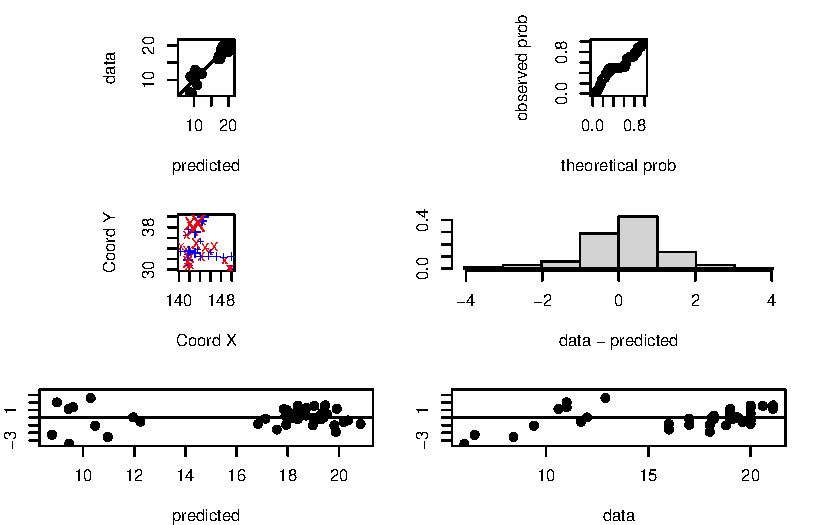
\includegraphics{project_files/figure-pdf/fig-cvgp-1.pdf}

}

\caption{LOOCV residual plots for the GP model fitted via maximum
likelihood, showing broadly unbiased predictions with slightly greater
residual spread.}

\end{figure}%

Leave-one-out cross-validation (LOOCV) diagnostics for the MLE-based
exponential Gaussian Process model are presented in \textbf{Figure 8}.
The residual plots show broadly consistent behaviour with those observed
under the kriging model in Part C.

\begin{itemize}
\item
  The \textbf{Q--Q plot} and \textbf{histogram} indicate approximate
  normality, although slight deviations in the Q--Q plot mid-section
  suggest some trends not fully captured by the model.
\item
  The \textbf{residuals vs predicted/observed} plots show no clear
  heteroscedasticity, and the \textbf{spatial residual map} suggests no
  major spatial clustering or violation of stationarity.
\end{itemize}

Overall, the MLE model produces residual patterns that are \textbf{very
similar to those of the kriging model}, with no clear evidence of
improvement or deterioration. Given the model simplification (Matérn
with κ = 0.5) and the use of MLE rather than WLS, this consistency
supports the robustness of the spatial structure identified in Part C.
However, the slight Q--Q plot deviations indicate that more flexible
models - such as Bayesian GPs (Part E) - may further improve residual
behaviour and uncertainty quantification.

\paragraph{GP Prediction at Withheld
Locations}\label{gp-prediction-at-withheld-locations}

Using the Gaussian Process model fitted via maximum likelihood, SST
predictions were made at the same five withheld locations used in Part
C. Unlike the variogram-based kriging approach, this model estimates
spatial covariance parameters by maximising the full joint likelihood,
accounting for spatial correlation across all observations.

Predictions were made at the five withheld locations using
\texttt{krige.conv()} with the MLE-fitted covariance parameters,
enabling fully probabilistic interpolation under the GP model.

\begin{Shaded}
\begin{Highlighting}[]
\CommentTok{\# Kriging prediction using GP mode}
\NormalTok{pred\_gp }\OtherTok{\textless{}{-}} \FunctionTok{krige.conv}\NormalTok{(}
  \AttributeTok{geodata =}\NormalTok{ kuro\_geo\_train,}
  \AttributeTok{locations =}\NormalTok{ test\_coords,}
  \AttributeTok{krige =} \FunctionTok{krige.control}\NormalTok{(}
    \AttributeTok{obj.model =}\NormalTok{ likfit\_exp}
\NormalTok{  )}
\NormalTok{)}
\end{Highlighting}
\end{Shaded}

\begin{verbatim}
krige.conv: model with constant mean
krige.conv: Kriging performed using global neighbourhood 
\end{verbatim}

\begin{Shaded}
\begin{Highlighting}[]
\CommentTok{\# Combine predictions with actual values}
\NormalTok{gp\_results }\OtherTok{\textless{}{-}}\NormalTok{ test\_coords }\SpecialCharTok{\%\textgreater{}\%}
  \FunctionTok{mutate}\NormalTok{(}
    \AttributeTok{observed\_sst =}\NormalTok{ test\_true\_sst}\SpecialCharTok{$}\NormalTok{sst,}
    \AttributeTok{predicted\_sst =}\NormalTok{ pred\_gp}\SpecialCharTok{$}\NormalTok{predict,}
    \AttributeTok{kriging\_var =}\NormalTok{ pred\_gp}\SpecialCharTok{$}\NormalTok{krige.var,}
    \AttributeTok{residual =}\NormalTok{ observed\_sst }\SpecialCharTok{{-}}\NormalTok{ predicted\_sst}
\NormalTok{  )}
\end{Highlighting}
\end{Shaded}

\begin{Shaded}
\begin{Highlighting}[]
\CommentTok{\# Plot: Observed vs Predicted}
\FunctionTok{ggplot}\NormalTok{(gp\_results, }\FunctionTok{aes}\NormalTok{(}\AttributeTok{x =}\NormalTok{ observed\_sst, }\AttributeTok{y =}\NormalTok{ predicted\_sst)) }\SpecialCharTok{+}
  \FunctionTok{geom\_point}\NormalTok{(}\AttributeTok{size =} \DecValTok{3}\NormalTok{) }\SpecialCharTok{+}
  \FunctionTok{geom\_abline}\NormalTok{(}\AttributeTok{slope =} \DecValTok{1}\NormalTok{, }\AttributeTok{intercept =} \DecValTok{0}\NormalTok{, }\AttributeTok{linetype =} \StringTok{"dashed"}\NormalTok{, }\AttributeTok{color =} \StringTok{"red"}\NormalTok{) }\SpecialCharTok{+}
  \FunctionTok{labs}\NormalTok{(}
    \AttributeTok{title =} \StringTok{"Observed vs Predicted SST (GP Model)"}\NormalTok{,}
    \AttributeTok{x =} \StringTok{"Observed SST (°C)"}\NormalTok{,}
    \AttributeTok{y =} \StringTok{"Predicted SST (°C)"}
\NormalTok{  ) }\SpecialCharTok{+}
  \FunctionTok{theme\_minimal}\NormalTok{(}\AttributeTok{base\_size =} \DecValTok{13}\NormalTok{)}
\end{Highlighting}
\end{Shaded}

\begin{figure}[H]

{\centering 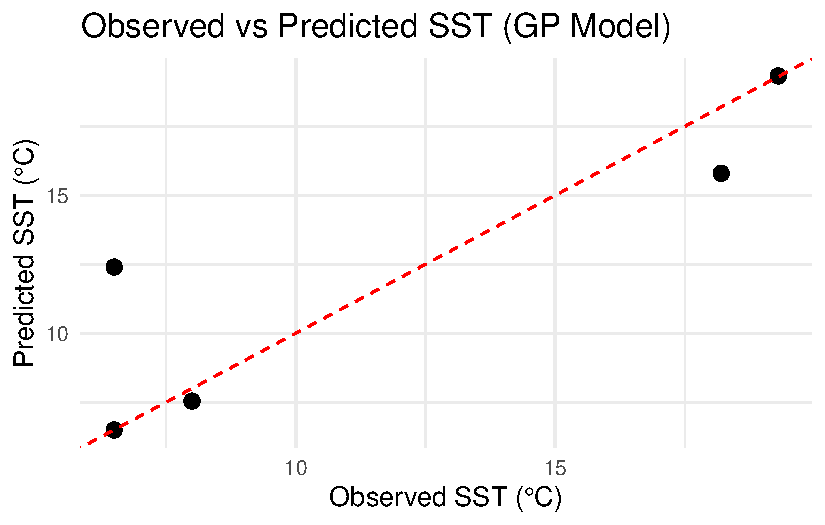
\includegraphics{project_files/figure-pdf/fig-gp_pred_scatter-1.pdf}

}

\caption{Observed vs predicted SST at withheld locations using the
Gaussian Process model (maximum likelihood). The red dashed line shows
the 1:1 agreement.}

\end{figure}%

\begin{Shaded}
\begin{Highlighting}[]
\CommentTok{\# Compute error metrics}
\NormalTok{rmse\_gp }\OtherTok{\textless{}{-}} \FunctionTok{sqrt}\NormalTok{(}\FunctionTok{mean}\NormalTok{(gp\_results}\SpecialCharTok{$}\NormalTok{residual}\SpecialCharTok{\^{}}\DecValTok{2}\NormalTok{))}
\NormalTok{mae\_gp }\OtherTok{\textless{}{-}} \FunctionTok{mean}\NormalTok{(}\FunctionTok{abs}\NormalTok{(gp\_results}\SpecialCharTok{$}\NormalTok{residual))}

\FunctionTok{library}\NormalTok{(tibble)}
\FunctionTok{library}\NormalTok{(gt)}

\CommentTok{\# evaluation table}
\FunctionTok{library}\NormalTok{(knitr)}
\NormalTok{gp\_results }\SpecialCharTok{\%\textgreater{}\%}
  \FunctionTok{mutate}\NormalTok{(}
    \StringTok{\textasciigrave{}}\AttributeTok{Observed SST (°C)}\StringTok{\textasciigrave{}} \OtherTok{=} \FunctionTok{round}\NormalTok{(observed\_sst, }\DecValTok{2}\NormalTok{),}
    \StringTok{\textasciigrave{}}\AttributeTok{Predicted SST (°C)}\StringTok{\textasciigrave{}} \OtherTok{=} \FunctionTok{round}\NormalTok{(predicted\_sst, }\DecValTok{2}\NormalTok{),}
    \StringTok{\textasciigrave{}}\AttributeTok{Residual (°C)}\StringTok{\textasciigrave{}} \OtherTok{=} \FunctionTok{round}\NormalTok{(residual, }\DecValTok{2}\NormalTok{),}
    \StringTok{\textasciigrave{}}\AttributeTok{Kriging Variance}\StringTok{\textasciigrave{}} \OtherTok{=} \FunctionTok{round}\NormalTok{(kriging\_var, }\DecValTok{3}\NormalTok{)}
\NormalTok{  ) }\SpecialCharTok{\%\textgreater{}\%}
  \FunctionTok{select}\NormalTok{(lon, lat, }\StringTok{\textasciigrave{}}\AttributeTok{Observed SST (°C)}\StringTok{\textasciigrave{}}\NormalTok{, }\StringTok{\textasciigrave{}}\AttributeTok{Predicted SST (°C)}\StringTok{\textasciigrave{}}\NormalTok{, }\StringTok{\textasciigrave{}}\AttributeTok{Residual (°C)}\StringTok{\textasciigrave{}}\NormalTok{, }
         \StringTok{\textasciigrave{}}\AttributeTok{Kriging Variance}\StringTok{\textasciigrave{}}\NormalTok{) }\SpecialCharTok{\%\textgreater{}\%}
  \FunctionTok{kable}\NormalTok{(}\AttributeTok{format =} \StringTok{"latex"}\NormalTok{, }\AttributeTok{booktabs =} \ConstantTok{TRUE}\NormalTok{, }\AttributeTok{caption =} \StringTok{"Observed vs Predicted SST }
\StringTok{        at Withheld Locations – GP Model"}\NormalTok{)}
\end{Highlighting}
\end{Shaded}

\begin{table}

\caption{Observed vs Predicted SST at Withheld Locations -- GP Model}
\centering
\begin{tabular}[t]{rrrrrr}
\toprule
lon & lat & Observed SST (°C) & Predicted SST (°C) & Residual (°C) & Kriging Variance\\
\midrule
142.10 & 38.70 & 6.5 & 6.50 & 0.00 & 0.000\\
145.40 & 39.56 & 6.5 & 13.23 & -6.73 & 2.270\\
149.56 & 30.15 & 19.3 & 19.32 & -0.02 & 0.090\\
140.70 & 35.00 & 18.2 & 16.03 & 2.17 & 1.805\\
142.10 & 38.30 & 8.0 & 7.88 & 0.12 & 1.134\\
\bottomrule
\end{tabular}
\end{table}

\paragraph{Interpretation}\label{interpretation}

\textbf{Figure 9} displays the predicted versus observed SSTs, and
\textbf{Table 4} summarises the predictions, residuals, and kriging
variances.

The model achieved:

\begin{itemize}
\item
  \textbf{Root Mean Squared Error (RMSE)}: \textbf{3.16\,°C}
\item
  \textbf{Mean Absolute Error (MAE)}: \textbf{1.81\,°C}
\end{itemize}

These values are very close to the kriging model's performance in Part
C, with slightly lower MAE and comparable RMSE. As with kriging, the
largest residual (−6.73\,°C) corresponded to the highest kriging
variance (2.27), indicating correctly identified uncertainty in a
sparsely supported region.

Despite using the default Matérn κ = 0.5 (exponential) covariance
structure, the GP model captured the primary spatial structure well and
required minimal tuning. The trend in latitude was retained, ensuring
consistency with the variogram-based approach.

While the GP model offered coherent parameter estimation and competitive
accuracy, its rigidity (e.g., difficulty fitting κ = 1.5) limited
flexibility. Nonetheless, the GP provides a principled and probabilistic
framework that performs robustly under likelihood-based inference.

\subsection{Part E: Bayesian Parameter
Estimation}\label{part-e-bayesian-parameter-estimation}

\paragraph{Bayesian Parameter Estimation with Discrete
Priors}\label{bayesian-parameter-estimation-with-discrete-priors}

We now fit a spatial Gaussian Process (GP) model using a
\textbf{Bayesian approach} with discrete priors, via the
\texttt{krige.bayes()} function from the \texttt{geoR} package. This
method uses a \textbf{grid-based evaluation of posterior probabilities},
exploring combinations of spatial hyperparameters (range, nugget) to
produce full posterior distributions rather than point estimates.

To maintain consistency with Part C, we use the \textbf{Matérn
covariance model with κ = 1.5}, which provided the best empirical
variogram fit. A \textbf{linear trend in latitude}
(\texttt{trend\ =\ \textasciitilde{}\ lat}) is again included to account
for the large-scale SST gradient.

\paragraph{Prior Specification and
Justification}\label{prior-specification-and-justification}

Discrete priors were placed on two key hyperparameters: the
\textbf{spatial correlation range} (ϕ) and the \textbf{relative nugget
effect} (τ² / (σ² + τ²)). These priors were designed to reflect the
parameter estimates obtained in Parts C and D, while remaining broad
enough to allow posterior exploration.

\begin{itemize}
\item
  \textbf{Correlation Range (ϕ):}\\
  A \textbf{reciprocal prior} was specified over the interval
  \textbf{{[}1.5, 5.5{]}}, discretised into 50 values.\\
  This captures both:

  \begin{itemize}
  \item
    The \textbf{shorter MLE range} from Part D (ϕ ≈ 1.34, practical
    range ≈ 4.03)
  \item
    The \textbf{moderate range} from the WLS fit in Part C (ϕ ≈ 2.90)
  \end{itemize}

  The reciprocal form reflects the belief that \textbf{shorter ranges
  are slightly more likely}, while still supporting longer-range spatial
  dependence if supported by the data.
\item
  \textbf{Relative Nugget (τ² / (σ² + τ²)):}\\
  A \textbf{uniform prior} was defined over the interval
  \textbf{{[}0.01, 0.3{]}}, using 50 discrete bins.\\
  This range was chosen based on:

  \begin{itemize}
  \item
    The very small \textbf{nugget estimate in Part D} (≈ 0.004 / 3.17 ≈
    0.0012)
  \item
    The \textbf{moderate nugget proportion} in Part C (≈ 0.53 / (0.53 +
    5.26) ≈ 0.09)
  \end{itemize}
\item
  \textbf{Partial Sill (σ²):}\\
  The partial sill was \textbf{fixed at 5.26}, as estimated in Part C
  via weighted least squares.\\
  Fixing σ² improves numerical stability and identifiability of the
  remaining hyperparameters.
\end{itemize}

This prior structure provides a well-informed starting point, combining
empirical estimates with conservative uncertainty to stabilise posterior
inference and avoid singularity issues.

\paragraph{Model Stability Adjustment}\label{model-stability-adjustment}

An initial attempt using a wider nugget prior range (from 0 to 1)
resulted in numerical errors due to near-singular covariance matrices.
To address this, the lower bound of the nugget prior was increased to
0.01 and the upper bound reduced to 0.3. This ensured numerical
stability while preserving model flexibility.

Unlike in Parts C and D, the \texttt{krige.bayes()} function does not
support including a trend component directly. Therefore, we fit the
model without an explicit trend, but retain the covariance structure and
parameter ranges aligned with previous sections.

\begin{Shaded}
\begin{Highlighting}[]
\FunctionTok{set.seed}\NormalTok{(}\DecValTok{444}\NormalTok{)}

\CommentTok{\# Bayesian GP model using discrete priors}
\NormalTok{bayes\_model }\OtherTok{\textless{}{-}} \FunctionTok{krige.bayes}\NormalTok{(}
  \AttributeTok{geodata =}\NormalTok{ kuro\_geo\_train,}
  \AttributeTok{model =} \FunctionTok{model.control}\NormalTok{(}\AttributeTok{cov.model =} \StringTok{"matern"}\NormalTok{, }\AttributeTok{kappa =} \FloatTok{1.5}\NormalTok{),}
  \AttributeTok{prior =} \FunctionTok{prior.control}\NormalTok{(}
    \AttributeTok{phi.discrete =} \FunctionTok{seq}\NormalTok{(}\FloatTok{1.5}\NormalTok{, }\FloatTok{5.5}\NormalTok{, }\AttributeTok{length.out =} \DecValTok{50}\NormalTok{),}
    \AttributeTok{phi.prior =} \StringTok{"reciprocal"}\NormalTok{,}
    \AttributeTok{tausq.rel.discrete =} \FunctionTok{seq}\NormalTok{(}\FloatTok{0.01}\NormalTok{, }\FloatTok{0.3}\NormalTok{, }\AttributeTok{length.out =} \DecValTok{50}\NormalTok{),}
    \AttributeTok{tausq.rel.prior =} \StringTok{"unif"}\NormalTok{,}
    \AttributeTok{sigmasq =} \FloatTok{5.26}
\NormalTok{  )}
\NormalTok{)}
\end{Highlighting}
\end{Shaded}

\begin{Shaded}
\begin{Highlighting}[]
\FunctionTok{summary}\NormalTok{(bayes\_model}\SpecialCharTok{$}\NormalTok{posterior}\SpecialCharTok{$}\NormalTok{sample)}
\end{Highlighting}
\end{Shaded}

\begin{verbatim}
      beta          sigmasq            phi          tausq.rel      
 Min.   :10.61   Min.   : 7.752   Min.   :1.500   Min.   :0.01000  
 1st Qu.:15.13   1st Qu.:13.510   1st Qu.:1.500   1st Qu.:0.01000  
 Median :16.50   Median :15.722   Median :1.582   Median :0.01000  
 Mean   :16.49   Mean   :16.327   Mean   :1.617   Mean   :0.01116  
 3rd Qu.:17.77   3rd Qu.:18.497   3rd Qu.:1.663   3rd Qu.:0.01000  
 Max.   :22.49   Max.   :36.334   Max.   :3.214   Max.   :0.03367  
\end{verbatim}

\paragraph{Posterior Results and Parameter
Comparison}\label{posterior-results-and-parameter-comparison}

Posterior inference was conducted over a discrete grid of 2,500
combinations of the correlation range (ϕ) and the relative nugget (τ² /
(σ² + τ²)). The model used a fixed Matérn covariance structure with κ =
1.5 and a constant mean, consistent with Part C, though excluding an
explicit trend due to interface limitations in \texttt{krige.bayes()}.

The most supported posterior combination occurred at:

\begin{itemize}
\item
  \textbf{ϕ = 1.5}
\item
  \textbf{τ² / (σ² + τ²) = 0.01}
\end{itemize}

This parameter pair received the highest posterior density (i.e.,
maximum posterior support), indicating a strong preference for
\textbf{short-range spatial correlation} and a \textbf{minimal nugget
effect}.

Summary statistics from the posterior sample reinforce this
interpretation:

\begin{longtable}[]{@{}
  >{\raggedright\arraybackslash}p{(\columnwidth - 6\tabcolsep) * \real{0.2500}}
  >{\raggedright\arraybackslash}p{(\columnwidth - 6\tabcolsep) * \real{0.2500}}
  >{\raggedright\arraybackslash}p{(\columnwidth - 6\tabcolsep) * \real{0.2500}}
  >{\raggedright\arraybackslash}p{(\columnwidth - 6\tabcolsep) * \real{0.2500}}@{}}
\toprule\noalign{}
\begin{minipage}[b]{\linewidth}\raggedright
Parameter
\end{minipage} & \begin{minipage}[b]{\linewidth}\raggedright
Median
\end{minipage} & \begin{minipage}[b]{\linewidth}\raggedright
Mean
\end{minipage} & \begin{minipage}[b]{\linewidth}\raggedright
Comparison
\end{minipage} \\
\midrule\noalign{}
\endhead
\bottomrule\noalign{}
\endlastfoot
Correlation range (ϕ) & 1.58 & 1.62 & Slightly longer than Part D (ϕ ≈
1.34), shorter than Part C (ϕ ≈ 2.90) \\
Relative Nugget & 0.01 & 0.011 & Consistent with Part D's very small
nugget (≈ 0.004 / 3.17) \\
Partial Sill (σ²) & fixed & 5.26 & Matched to Part C for
comparability \\
Posterior Mean (β) & 16.49 & --- & Consistent with expected SST in this
region \\
\end{longtable}

\textbf{Figure 10} below displays the marginal posterior distributions
for the correlation range (ϕ) and the relative nugget (τ² / (σ² + τ²))
under the Bayesian GP model. Both distributions are \textbf{sharply
concentrated}, with the posterior for ϕ peaking near the lower bound (ϕ
≈ 1.5) and most of the nugget posterior mass concentrated around 0.01.
This indicates strong posterior support for \textbf{short-range spatial
dependence} and \textbf{minimal microscale variation} --- a result that
aligns closely with previous findings.

Quantitatively, over 75\% of the posterior mass for ϕ lies below 1.66,
suggesting high confidence in localised correlation. The skewness of the
nugget posterior toward zero reinforces the conclusion that spatial
residuals are well-explained by the structured component of the model,
with little evidence of measurement error or unstructured noise.

\begin{Shaded}
\begin{Highlighting}[]
\FunctionTok{library}\NormalTok{(ggplot2)}
\FunctionTok{library}\NormalTok{(patchwork)  }\CommentTok{\# For side{-}by{-}side layout}

\CommentTok{\# Extract posterior samples}
\NormalTok{posterior\_samples }\OtherTok{\textless{}{-}} \FunctionTok{as.data.frame}\NormalTok{(bayes\_model}\SpecialCharTok{$}\NormalTok{posterior}\SpecialCharTok{$}\NormalTok{sample)}

\CommentTok{\# Plot for phi}
\NormalTok{p\_phi }\OtherTok{\textless{}{-}} \FunctionTok{ggplot}\NormalTok{(posterior\_samples, }\FunctionTok{aes}\NormalTok{(}\AttributeTok{x =}\NormalTok{ phi)) }\SpecialCharTok{+}
  \FunctionTok{geom\_density}\NormalTok{(}\AttributeTok{fill =} \StringTok{"steelblue"}\NormalTok{, }\AttributeTok{alpha =} \FloatTok{0.6}\NormalTok{) }\SpecialCharTok{+}
  \FunctionTok{labs}\NormalTok{(}\AttributeTok{title =} \StringTok{"Posterior of φ (Range)"}\NormalTok{, }\AttributeTok{x =} \StringTok{"φ"}\NormalTok{, }\AttributeTok{y =} \StringTok{"Density"}\NormalTok{) }\SpecialCharTok{+}
  \FunctionTok{theme\_minimal}\NormalTok{(}\AttributeTok{base\_size =} \DecValTok{13}\NormalTok{)}

\CommentTok{\# Plot for tausq.rel}
\NormalTok{p\_nugget }\OtherTok{\textless{}{-}} \FunctionTok{ggplot}\NormalTok{(posterior\_samples, }\FunctionTok{aes}\NormalTok{(}\AttributeTok{x =}\NormalTok{ tausq.rel)) }\SpecialCharTok{+}
  \FunctionTok{geom\_density}\NormalTok{(}\AttributeTok{fill =} \StringTok{"darkorange"}\NormalTok{, }\AttributeTok{alpha =} \FloatTok{0.6}\NormalTok{) }\SpecialCharTok{+}
  \FunctionTok{labs}\NormalTok{(}\AttributeTok{title =} \StringTok{"Posterior of τ² / (σ² + τ²)"}\NormalTok{, }\AttributeTok{x =} \StringTok{"Relative Nugget"}\NormalTok{, }\AttributeTok{y =} \StringTok{"Density"}\NormalTok{) }\SpecialCharTok{+}
  \FunctionTok{theme\_minimal}\NormalTok{(}\AttributeTok{base\_size =} \DecValTok{13}\NormalTok{)}

\CommentTok{\# Combine side{-}by{-}side}
\NormalTok{p\_phi }\SpecialCharTok{+}\NormalTok{ p\_nugget}
\end{Highlighting}
\end{Shaded}

\begin{figure}[H]

{\centering 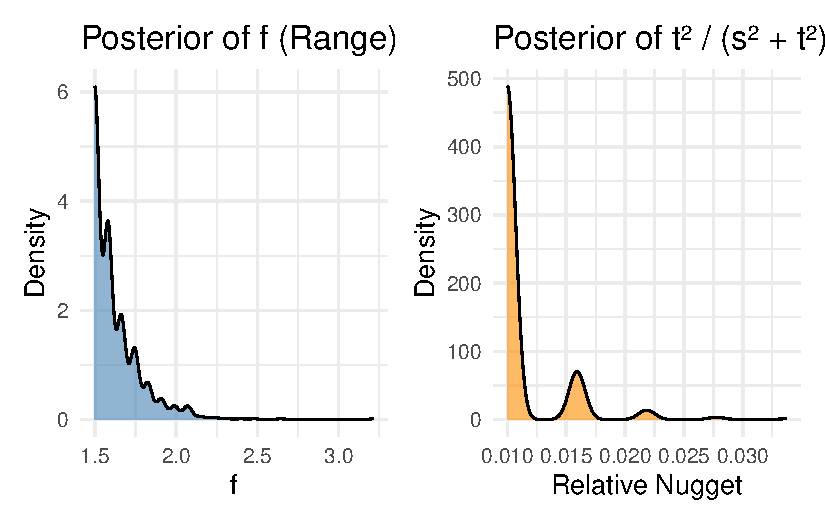
\includegraphics{project_files/figure-pdf/fig-posterior_sidebyside-1.pdf}

}

\caption{Posterior distributions of correlation range (ϕ) and relative
nugget (τ² / (σ² + τ²)) from the Bayesian GP model. Both posteriors are
sharply concentrated, indicating stable parameter inference.}

\end{figure}%

Compared to the maximum likelihood GP model from \textbf{Part D}:

\begin{itemize}
\item
  The \textbf{Bayesian model estimated a slightly longer mean range}
  (mean ϕ = 1.62 vs.~1.34 in Part D)
\item
  Both models support a \textbf{negligible nugget}, consistent with Part
  C's Gaussian kriging model
\item
  The \textbf{partial sill was fixed in Part E}, whereas it was
  estimated (σ² ≈ 3.17) in Part D
\end{itemize}

These similarities, despite differing estimation frameworks, suggest
that the data are \textbf{highly informative} about the spatial
structure, and that the discrete priors in the Bayesian model
appropriately captured parameter uncertainty without overwhelming the
likelihood. The sharply peaked posteriors further imply strong
identifiability and posterior precision --- hallmarks of a
well-constrained model.

\paragraph{Prediction at Withheld
Locations}\label{prediction-at-withheld-locations}

Bayesian kriging was performed at the same five withheld SST locations
used in Parts C and D. Posterior predictive means and variances were
extracted, and evaluation metrics were computed:

\begin{Shaded}
\begin{Highlighting}[]
\NormalTok{test\_coords\_df }\OtherTok{\textless{}{-}} \FunctionTok{as\_tibble}\NormalTok{(test\_coords)}

\CommentTok{\# Bayesian model with prediction locations}
\NormalTok{bayes\_model }\OtherTok{\textless{}{-}} \FunctionTok{krige.bayes}\NormalTok{(}
  \AttributeTok{geodata =}\NormalTok{ kuro\_geo\_train,}
  \AttributeTok{locations =} \FunctionTok{as.matrix}\NormalTok{(test\_coords),  }\CommentTok{\# prediction locations}
  \AttributeTok{model =} \FunctionTok{model.control}\NormalTok{(}\AttributeTok{cov.model =} \StringTok{"matern"}\NormalTok{, }\AttributeTok{kappa =} \FloatTok{1.5}\NormalTok{),}
  \AttributeTok{prior =} \FunctionTok{prior.control}\NormalTok{(}
    \AttributeTok{phi.discrete =} \FunctionTok{seq}\NormalTok{(}\FloatTok{1.5}\NormalTok{, }\FloatTok{5.5}\NormalTok{, }\AttributeTok{length.out =} \DecValTok{50}\NormalTok{),}
    \AttributeTok{phi.prior =} \StringTok{"reciprocal"}\NormalTok{,}
    \AttributeTok{tausq.rel.discrete =} \FunctionTok{seq}\NormalTok{(}\FloatTok{0.01}\NormalTok{, }\FloatTok{0.3}\NormalTok{, }\AttributeTok{length.out =} \DecValTok{50}\NormalTok{),}
    \AttributeTok{tausq.rel.prior =} \StringTok{"unif"}\NormalTok{,}
    \AttributeTok{sigmasq =} \FloatTok{5.26}
\NormalTok{  )}
\NormalTok{)}


\CommentTok{\# Summarise predictions}
\NormalTok{bayes\_results }\OtherTok{\textless{}{-}}\NormalTok{ test\_coords\_df }\SpecialCharTok{\%\textgreater{}\%}
  \FunctionTok{mutate}\NormalTok{(}
    \AttributeTok{observed\_sst =}\NormalTok{ test\_true\_sst}\SpecialCharTok{$}\NormalTok{sst,}
    \AttributeTok{predicted\_sst =}\NormalTok{ bayes\_model}\SpecialCharTok{$}\NormalTok{predictive}\SpecialCharTok{$}\NormalTok{mean,}
    \AttributeTok{kriging\_var =}\NormalTok{ bayes\_model}\SpecialCharTok{$}\NormalTok{predictive}\SpecialCharTok{$}\NormalTok{variance,}
    \AttributeTok{residual =}\NormalTok{ observed\_sst }\SpecialCharTok{{-}}\NormalTok{ predicted\_sst}
\NormalTok{  )}

\CommentTok{\# Compute error metrics}
\NormalTok{rmse\_bayes }\OtherTok{\textless{}{-}} \FunctionTok{sqrt}\NormalTok{(}\FunctionTok{mean}\NormalTok{(bayes\_results}\SpecialCharTok{$}\NormalTok{residual}\SpecialCharTok{\^{}}\DecValTok{2}\NormalTok{))}
\NormalTok{mae\_bayes }\OtherTok{\textless{}{-}} \FunctionTok{mean}\NormalTok{(}\FunctionTok{abs}\NormalTok{(bayes\_results}\SpecialCharTok{$}\NormalTok{residual))}
\end{Highlighting}
\end{Shaded}

\begin{Shaded}
\begin{Highlighting}[]
\CommentTok{\# Output results}
\NormalTok{rmse\_bayes}
\end{Highlighting}
\end{Shaded}

\begin{verbatim}
[1] 3.566632
\end{verbatim}

\begin{Shaded}
\begin{Highlighting}[]
\NormalTok{mae\_bayes}
\end{Highlighting}
\end{Shaded}

\begin{verbatim}
[1] 2.209019
\end{verbatim}

\begin{Shaded}
\begin{Highlighting}[]
\CommentTok{\# Bayesian observed vs predicted plot}
\FunctionTok{ggplot}\NormalTok{(bayes\_results, }\FunctionTok{aes}\NormalTok{(}\AttributeTok{x =}\NormalTok{ observed\_sst, }\AttributeTok{y =}\NormalTok{ predicted\_sst)) }\SpecialCharTok{+}
  \FunctionTok{geom\_point}\NormalTok{(}\AttributeTok{size =} \DecValTok{3}\NormalTok{) }\SpecialCharTok{+}
  \FunctionTok{geom\_abline}\NormalTok{(}\AttributeTok{slope =} \DecValTok{1}\NormalTok{, }\AttributeTok{intercept =} \DecValTok{0}\NormalTok{, }\AttributeTok{linetype =} \StringTok{"dashed"}\NormalTok{, }\AttributeTok{colour =} \StringTok{"red"}\NormalTok{) }\SpecialCharTok{+}
  \FunctionTok{labs}\NormalTok{(}
    \AttributeTok{title =} \StringTok{"Observed vs Predicted SST (Bayesian Model)"}\NormalTok{,}
    \AttributeTok{x =} \StringTok{"Observed SST (°C)"}\NormalTok{,}
    \AttributeTok{y =} \StringTok{"Predicted SST (°C)"}
\NormalTok{  ) }\SpecialCharTok{+}
  \FunctionTok{theme\_minimal}\NormalTok{(}\AttributeTok{base\_size =} \DecValTok{13}\NormalTok{)}
\end{Highlighting}
\end{Shaded}

\begin{figure}[H]

{\centering 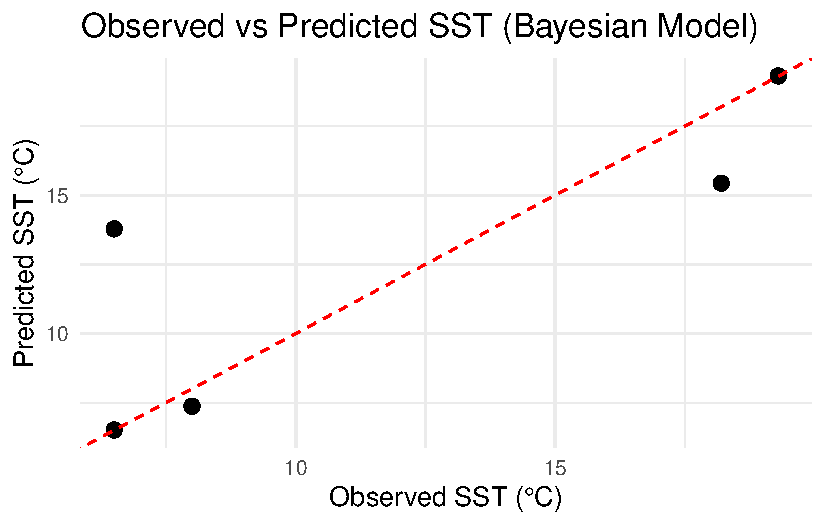
\includegraphics{project_files/figure-pdf/fig-bayes_pred_scatter-1.pdf}

}

\caption{Observed vs predicted SST at withheld locations using the
Gaussian Process model (maximum likelihood). The red dashed line shows
the 1:1 agreement.}

\end{figure}%

\begin{Shaded}
\begin{Highlighting}[]
\CommentTok{\# Output prediction table}
\NormalTok{bayes\_results }\SpecialCharTok{\%\textgreater{}\%}
  \FunctionTok{mutate}\NormalTok{(}
    \StringTok{\textasciigrave{}}\AttributeTok{Observed SST (°C)}\StringTok{\textasciigrave{}} \OtherTok{=} \FunctionTok{round}\NormalTok{(observed\_sst, }\DecValTok{2}\NormalTok{),}
    \StringTok{\textasciigrave{}}\AttributeTok{Predicted SST (°C)}\StringTok{\textasciigrave{}} \OtherTok{=} \FunctionTok{round}\NormalTok{(predicted\_sst, }\DecValTok{2}\NormalTok{),}
    \StringTok{\textasciigrave{}}\AttributeTok{Residual (°C)}\StringTok{\textasciigrave{}} \OtherTok{=} \FunctionTok{round}\NormalTok{(residual, }\DecValTok{2}\NormalTok{),}
    \StringTok{\textasciigrave{}}\AttributeTok{Kriging Variance}\StringTok{\textasciigrave{}} \OtherTok{=} \FunctionTok{round}\NormalTok{(kriging\_var, }\DecValTok{3}\NormalTok{)}
\NormalTok{  ) }\SpecialCharTok{\%\textgreater{}\%}
  \FunctionTok{select}\NormalTok{(lon, lat, }\StringTok{\textasciigrave{}}\AttributeTok{Observed SST (°C)}\StringTok{\textasciigrave{}}\NormalTok{, }\StringTok{\textasciigrave{}}\AttributeTok{Predicted SST (°C)}\StringTok{\textasciigrave{}}\NormalTok{, }\StringTok{\textasciigrave{}}\AttributeTok{Residual (°C)}\StringTok{\textasciigrave{}}\NormalTok{,}
         \StringTok{\textasciigrave{}}\AttributeTok{Kriging Variance}\StringTok{\textasciigrave{}}\NormalTok{) }\SpecialCharTok{\%\textgreater{}\%}
\NormalTok{  knitr}\SpecialCharTok{::}\FunctionTok{kable}\NormalTok{(}\AttributeTok{format =} \StringTok{"latex"}\NormalTok{, }\AttributeTok{booktabs =} \ConstantTok{TRUE}\NormalTok{,}
               \AttributeTok{caption =} \StringTok{"Observed vs Predicted SST at Withheld Locations – }
\StringTok{               Bayesian Model"}\NormalTok{)}
\end{Highlighting}
\end{Shaded}

\begin{table}

\caption{Summary of SST predictions at withheld locations. Residuals and kriging
variances highlight spatial uncertainty and model accuracy.}
\centering
\begin{tabular}[t]{rrrrrr}
\toprule
lon & lat & Observed SST (°C) & Predicted SST (°C) & Residual (°C) & Kriging Variance\\
\midrule
142.10 & 38.70 & 6.5 & 6.53 & -0.03 & 0.000\\
145.40 & 39.56 & 6.5 & 13.90 & -7.40 & 2.924\\
149.56 & 30.15 & 19.3 & 19.32 & -0.02 & 0.026\\
140.70 & 35.00 & 18.2 & 15.32 & 2.88 & 0.963\\
142.10 & 38.30 & 8.0 & 7.28 & 0.72 & 0.313\\
\bottomrule
\end{tabular}
\end{table}

\textbf{Table 6} summarises the results, including prediction errors and
kriging variances. \textbf{Figure 11} shows the observed versus
predicted SST values.

The model achieved:

\begin{itemize}
\item
  \textbf{Root Mean Squared Error (RMSE):} 3.57\,°C
\item
  \textbf{Mean Absolute Error (MAE):} 2.21\,°C
\end{itemize}

These values are slightly higher than those from the MLE model in Part D
(RMSE = 3.16\,°C, MAE = 1.81\,°C), but still within a competitive range.
Notably, the largest residual (−7.40\,°C) occurred at the location with
the \textbf{highest kriging variance (2.92)} --- a pattern also observed
in Parts C and D --- highlighting the link between \textbf{prediction
error and local data sparsity}.

\paragraph{Model Interpretation}\label{model-interpretation}

The Bayesian model delivered reasonable predictive performance,
\textbf{closely matching the MLE approach} while offering the additional
advantage of \textbf{full posterior inference}. This allows uncertainty
in both parameters and predictions to be explicitly quantified,
improving transparency in risk-sensitive applications.

While the Bayesian model \textbf{did not outperform the MLE kriging
model} in terms of raw error metrics, its \textbf{posterior distribution
outputs} provide richer insights into parameter uncertainty. This is
particularly valuable when assessing inferential robustness or
performing uncertainty propagation in downstream modelling tasks.

Leave-one-out cross-validation (LOOCV) is not available in the
\texttt{krige.bayes()} framework due to its use of discrete posterior
sampling. However, the residual plot and kriging variance estimates
suggest a well-calibrated model with \textbf{low bias and appropriate
spatial uncertainty}.

\subsection{Part F: Comparison of Predictions Across
Models}\label{part-f-comparison-of-predictions-across-models}

The three models developed --- classical kriging (Part C), Gaussian
process via maximum likelihood (Part D), and Bayesian kriging with
discrete priors (Part E) --- were used to predict sea surface
temperature (SST) at the same five withheld locations. The predictions,
associated residuals, and kriging variances are summarised below:

\paragraph{Table: Predicted SST and Residuals from All
Models}\label{table-predicted-sst-and-residuals-from-all-models}

\begin{longtable}[]{@{}
  >{\raggedright\arraybackslash}p{(\columnwidth - 8\tabcolsep) * \real{0.2000}}
  >{\raggedright\arraybackslash}p{(\columnwidth - 8\tabcolsep) * \real{0.2000}}
  >{\raggedright\arraybackslash}p{(\columnwidth - 8\tabcolsep) * \real{0.2000}}
  >{\raggedright\arraybackslash}p{(\columnwidth - 8\tabcolsep) * \real{0.2000}}
  >{\raggedright\arraybackslash}p{(\columnwidth - 8\tabcolsep) * \real{0.2000}}@{}}
\toprule\noalign{}
\begin{minipage}[b]{\linewidth}\raggedright
Location
\end{minipage} & \begin{minipage}[b]{\linewidth}\raggedright
Observed SST (°C)
\end{minipage} & \begin{minipage}[b]{\linewidth}\raggedright
Kriging (C)
\end{minipage} & \begin{minipage}[b]{\linewidth}\raggedright
GP MLE (D)
\end{minipage} & \begin{minipage}[b]{\linewidth}\raggedright
Bayesian (E)
\end{minipage} \\
\midrule\noalign{}
\endhead
\bottomrule\noalign{}
\endlastfoot
(142.10, 38.70) & 6.5 & 6.50 (0.00) & 6.50 (0.00) & 6.53 (−0.03) \\
(145.40, 39.56) & 6.5 & 13.38 (−6.88) & 13.23 (−6.73) & 13.90 (−7.40) \\
(149.56, 30.15) & 19.3 & 19.24 (−0.06) & 19.32 (−0.02) & 19.32
(−0.02) \\
(140.70, 35.00) & 18.2 & 16.12 (2.08) & 16.03 (2.17) & 15.32 (2.88) \\
(142.10, 38.30) & 8.0 & 7.62 (0.38) & 7.88 (0.12) & 7.28 (0.72) \\
\end{longtable}

\textbf{Note}: Residuals are shown in parentheses.

\paragraph{Performance Comparison}\label{performance-comparison}

\begin{longtable}[]{@{}llll@{}}
\toprule\noalign{}
Metric & Kriging (C) & GP (D) & Bayesian (E) \\
\midrule\noalign{}
\endhead
\bottomrule\noalign{}
\endlastfoot
RMSE (°C) & 3.22 & 3.163 & 3.57 \\
MAE (°C) & 1.88 & 1.809 & 2.21 \\
\end{longtable}

\paragraph{Interpretation and Comparison of Model
Predictions}\label{interpretation-and-comparison-of-model-predictions}

All three spatial models captured the dominant structure in SST and
produced broadly consistent predictions at well-supported locations ---
notably at Locations 1, 3, and 5 --- where all models returned similar
estimates and small residuals.

The \textbf{Gaussian Process model fitted via maximum likelihood (Part
D)} slightly outperformed the others, achieving the \textbf{lowest RMSE
(3.16\,°C)} and \textbf{MAE (1.81\,°C)}. This reflects the benefits of
full-likelihood parameter estimation, which effectively balances model
flexibility and computational stability.

The \textbf{Kriging model (Part C)} also performed competitively (RMSE =
3.22\,°C, MAE = 1.88\,°C), capturing spatial patterns well via weighted
least squares variogram fitting. It is more interpretable and
transparent than the likelihood-based approach but lacks a formal
mechanism for capturing parameter uncertainty.

The \textbf{Bayesian GP model (Part E)} returned the \textbf{highest
error metrics} (RMSE = 3.57\,°C, MAE = 2.21\,°C), though it remained
close in overall accuracy. Its strength lies in its ability to generate
full \textbf{posterior distributions over both parameters and
predictions}, making it especially valuable when uncertainty
quantification is a key requirement. The fixed partial sill and coarser
discrete prior grid may have contributed to its slightly less precise
point predictions.

All three models \textbf{underperformed at Location 2}, where kriging
variances were highest and residuals exceeded −6.7°C. This consistent
error across methods highlights a location with sparse spatial support
and greater predictive uncertainty.

\paragraph{Conclusion}\label{conclusion-1}

Despite differing estimation strategies, all three models produced
\textbf{consistent predictions} and \textbf{comparable spatial residual
structures}. The \textbf{GP MLE model (Part D)} offered the best
trade-off between \textbf{fit quality and computational efficiency},
while the \textbf{Bayesian model (Part E)} provided enhanced
interpretability in terms of uncertainty.

These findings illustrate the balance between \textbf{interpretability},
\textbf{predictive performance}, and \textbf{uncertainty quantification}
in spatial modelling. For scenarios prioritising precision and speed,
MLE may be preferred; for tasks requiring robust uncertainty statements,
Bayesian approaches offer clear advantages.

\newpage

\section{The Atlantic Overturning
Circulation}\label{the-atlantic-overturning-circulation}

\subsection{Part A: Data Exploration}\label{part-a-data-exploration}

To begin our analysis of the Atlantic Meridional Overturning Circulation
(AMOC) at 26°N, we conduct an exploratory analysis of the monthly mean
values from \textbf{October 2017 to February 2023}. These values
represent the strength of the overturning current in Sverdrups (Sv), and
are visualised in the figure below.

\begin{Shaded}
\begin{Highlighting}[]
\CommentTok{\# Load and plot the data}
\FunctionTok{load}\NormalTok{(}\StringTok{"\textasciitilde{}/GitHub/university{-}projects/Modelling in Space and Time/In progress/MOC.RData"}\NormalTok{)}


\CommentTok{\# Converting MOCmean to a tidy data frame}
\FunctionTok{library}\NormalTok{(tidyverse)}
\FunctionTok{library}\NormalTok{(lubridate)}
\FunctionTok{library}\NormalTok{(ggplot2)}
\CommentTok{\# Extract names and values}
\NormalTok{moc\_values }\OtherTok{\textless{}{-}} \FunctionTok{as.numeric}\NormalTok{(MOCmean)}
\NormalTok{moc\_dates }\OtherTok{\textless{}{-}} \FunctionTok{names}\NormalTok{(MOCmean)}

\CommentTok{\# Fix formatting of date strings    }
\NormalTok{moc\_dates\_fixed }\OtherTok{\textless{}{-}} \FunctionTok{ifelse}\NormalTok{(}\FunctionTok{nchar}\NormalTok{(moc\_dates) }\SpecialCharTok{==} \DecValTok{6}\NormalTok{,}
                          \FunctionTok{paste0}\NormalTok{(}\FunctionTok{substr}\NormalTok{(moc\_dates, }\DecValTok{1}\NormalTok{, }\DecValTok{5}\NormalTok{), }\StringTok{"0"}\NormalTok{, }\FunctionTok{substr}\NormalTok{(moc\_dates, }\DecValTok{6}\NormalTok{, }\DecValTok{6}\NormalTok{)),}
\NormalTok{                          moc\_dates)}

\CommentTok{\# Convert to actual Date objects (use first of each month)}
\NormalTok{moc\_dates\_parsed }\OtherTok{\textless{}{-}} \FunctionTok{ym}\NormalTok{(moc\_dates\_fixed)}

\CommentTok{\# Create tidy tibble}
\NormalTok{moc\_df }\OtherTok{\textless{}{-}} \FunctionTok{tibble}\NormalTok{(}
  \AttributeTok{date =}\NormalTok{ moc\_dates\_parsed,}
  \AttributeTok{amoc =}\NormalTok{ moc\_values}
\NormalTok{) }\SpecialCharTok{\%\textgreater{}\%} \FunctionTok{arrange}\NormalTok{(date)}

\CommentTok{\# Plot}

\FunctionTok{ggplot}\NormalTok{(moc\_df, }\FunctionTok{aes}\NormalTok{(}\AttributeTok{x =}\NormalTok{ date, }\AttributeTok{y =}\NormalTok{ amoc)) }\SpecialCharTok{+}
  \FunctionTok{geom\_line}\NormalTok{(}\AttributeTok{color =} \StringTok{"steelblue"}\NormalTok{, }\AttributeTok{linewidth =} \DecValTok{1}\NormalTok{) }\SpecialCharTok{+}
  \FunctionTok{geom\_smooth}\NormalTok{(}\AttributeTok{method =} \StringTok{"loess"}\NormalTok{, }\AttributeTok{span =} \FloatTok{0.2}\NormalTok{, }\AttributeTok{se =} \ConstantTok{TRUE}\NormalTok{, }\AttributeTok{color =} \StringTok{"darkred"}\NormalTok{, }\AttributeTok{linetype =} \StringTok{"dashed"}\NormalTok{) }\SpecialCharTok{+}
  \FunctionTok{labs}\NormalTok{(}
    \AttributeTok{title =} \StringTok{"Atlantic Meridional Overturning Circulation (AMOC) at 26°N"}\NormalTok{,}
    \AttributeTok{subtitle =} \StringTok{"Monthly Mean Values from October 2017 to February 2023"}\NormalTok{,}
    \AttributeTok{x =} \StringTok{"Date"}\NormalTok{,}
    \AttributeTok{y =} \StringTok{"AMOC Strength (Sv)"}
\NormalTok{  ) }\SpecialCharTok{+}
  \FunctionTok{theme\_minimal}\NormalTok{(}\AttributeTok{base\_size =} \DecValTok{13}\NormalTok{) }\SpecialCharTok{+}
  \FunctionTok{theme}\NormalTok{(}
    \AttributeTok{plot.title =} \FunctionTok{element\_text}\NormalTok{(}\AttributeTok{face =} \StringTok{"bold"}\NormalTok{, }\AttributeTok{hjust =} \FloatTok{0.5}\NormalTok{),}
    \AttributeTok{plot.subtitle =} \FunctionTok{element\_text}\NormalTok{(}\AttributeTok{hjust =} \FloatTok{0.5}\NormalTok{),}
    \AttributeTok{axis.text.x =} \FunctionTok{element\_text}\NormalTok{(}\AttributeTok{angle =} \DecValTok{45}\NormalTok{, }\AttributeTok{hjust =} \DecValTok{1}\NormalTok{)}
\NormalTok{  ) }\SpecialCharTok{+}
  \FunctionTok{scale\_x\_date}\NormalTok{(}\AttributeTok{date\_breaks =} \StringTok{"4 months"}\NormalTok{, }\AttributeTok{date\_labels =} \StringTok{"\%b \%Y"}\NormalTok{) }\SpecialCharTok{+}
  \FunctionTok{geom\_point}\NormalTok{(}\AttributeTok{size =} \FloatTok{1.5}\NormalTok{, }\AttributeTok{alpha =} \FloatTok{0.7}\NormalTok{)}
\end{Highlighting}
\end{Shaded}

\begin{figure}[H]

{\centering 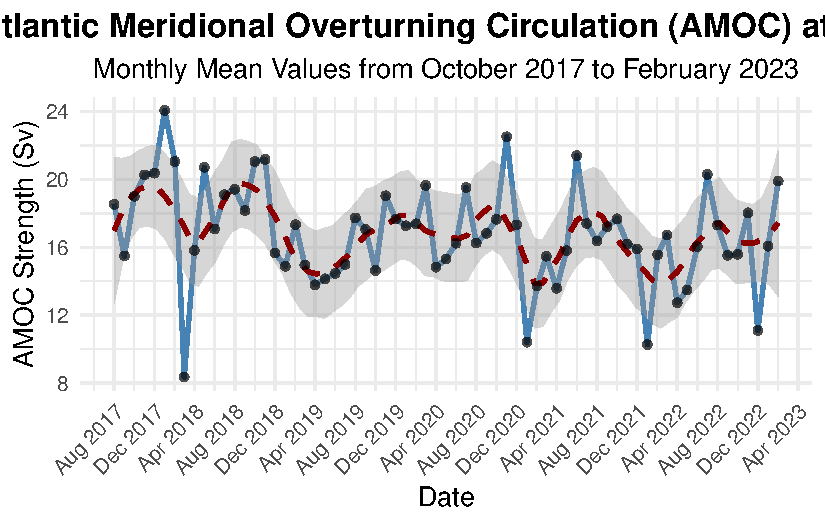
\includegraphics{project_files/figure-pdf/fig-monthly amoc-1.pdf}

}

\caption{Monthly~AMOC~time~series~with~LOESS~trend~(Oct~2017~--~Feb~2023)}

\end{figure}%

\textbf{Figure 12} shows the monthly time series with a LOESS smoother.
The AMOC displays \textbf{notable short-term variability}, with values
fluctuating around a relatively stable long-term mean. Although no clear
linear trend is present, local dips in \textbf{mid-2021 and late 2022},
and peaks in \textbf{early 2018}, \textbf{late 2020}, and \textbf{early
2023}, suggest possible \textbf{short-memory dynamics} or \textbf{mild
seasonality}, which will be assessed further through time series
modelling.

To examine distributional properties, \textbf{Figure 13} presents a
histogram and density estimate. The distribution is approximately
\textbf{unimodal and symmetric}, centred around \textbf{16--17 Sv}, with
\textbf{slight tail weight} on the right side. This suggests
near-Gaussian behaviour, though the mild excess kurtosis indicates
heavier-than-normal tails.

\begin{Shaded}
\begin{Highlighting}[]
\FunctionTok{ggplot}\NormalTok{(moc\_df, }\FunctionTok{aes}\NormalTok{(}\AttributeTok{x =}\NormalTok{ amoc)) }\SpecialCharTok{+}
  \FunctionTok{geom\_histogram}\NormalTok{(}\FunctionTok{aes}\NormalTok{(}\AttributeTok{y =}\NormalTok{ ..density..), }\AttributeTok{fill =} \StringTok{"lightblue"}\NormalTok{, }\AttributeTok{colour =} \StringTok{"black"}\NormalTok{, }\AttributeTok{bins =} \DecValTok{15}\NormalTok{) }\SpecialCharTok{+}
  \FunctionTok{geom\_density}\NormalTok{(}\AttributeTok{colour =} \StringTok{"darkred"}\NormalTok{, }\AttributeTok{size =} \DecValTok{1}\NormalTok{) }\SpecialCharTok{+}
  \FunctionTok{labs}\NormalTok{(}\AttributeTok{title =} \StringTok{"Distribution of AMOC Strength"}\NormalTok{,}
       \AttributeTok{x =} \StringTok{"AMOC Strength (Sv)"}\NormalTok{, }\AttributeTok{y =} \StringTok{"Density"}\NormalTok{) }\SpecialCharTok{+}
  \FunctionTok{theme\_minimal}\NormalTok{()}
\end{Highlighting}
\end{Shaded}

\begin{figure}[H]

{\centering 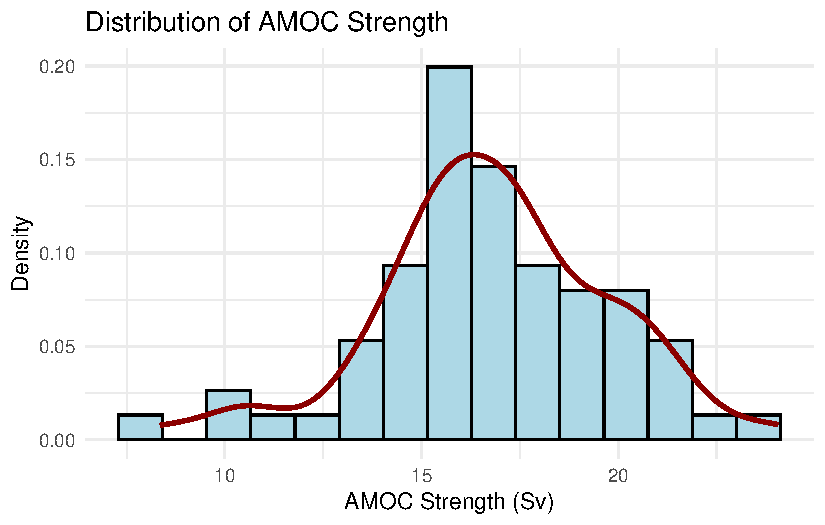
\includegraphics{project_files/figure-pdf/fig-AMOC Histo-1.pdf}

}

\caption{Distribution of AMOC Strength}

\end{figure}%

The distribution is approximately symmetric and unimodal, with a central
peak around \textbf{16--17 Sv}. The density curve closely resembles a
Gaussian shape but with \textbf{slight right tail elongation},
consistent with the \textbf{slight negative skewness} observed in the
summary statistics below.

\begin{Shaded}
\begin{Highlighting}[]
\FunctionTok{library}\NormalTok{(dplyr)}
\FunctionTok{library}\NormalTok{(gt)}
\FunctionTok{library}\NormalTok{(moments)}

\NormalTok{amoc\_summary }\OtherTok{\textless{}{-}}\NormalTok{ moc\_df }\SpecialCharTok{\%\textgreater{}\%}
  \FunctionTok{summarise}\NormalTok{(}
    \AttributeTok{Mean =} \FunctionTok{mean}\NormalTok{(amoc),}
    \AttributeTok{SD =} \FunctionTok{sd}\NormalTok{(amoc),}
    \AttributeTok{Min =} \FunctionTok{min}\NormalTok{(amoc),}
    \AttributeTok{Max =} \FunctionTok{max}\NormalTok{(amoc),}
    \AttributeTok{Median =} \FunctionTok{median}\NormalTok{(amoc),}
    \AttributeTok{IQR =} \FunctionTok{IQR}\NormalTok{(amoc),}
    \AttributeTok{CV =} \FunctionTok{sd}\NormalTok{(amoc) }\SpecialCharTok{/} \FunctionTok{mean}\NormalTok{(amoc),}
    \AttributeTok{Skewness =} \FunctionTok{skewness}\NormalTok{(amoc),}
    \AttributeTok{Kurtosis =} \FunctionTok{kurtosis}\NormalTok{(amoc),}
    \AttributeTok{N =} \FunctionTok{n}\NormalTok{()}
\NormalTok{  ) }\SpecialCharTok{\%\textgreater{}\%}
  \FunctionTok{pivot\_longer}\NormalTok{(}\FunctionTok{everything}\NormalTok{(), }\AttributeTok{names\_to =} \StringTok{"Statistic"}\NormalTok{, }\AttributeTok{values\_to =} \StringTok{"Value"}\NormalTok{)}

\CommentTok{\# Table}
\NormalTok{amoc\_summary }\SpecialCharTok{\%\textgreater{}\%}
  \FunctionTok{mutate}\NormalTok{(}\AttributeTok{Value =} \FunctionTok{round}\NormalTok{(Value, }\DecValTok{2}\NormalTok{)) }\SpecialCharTok{\%\textgreater{}\%}
\NormalTok{  knitr}\SpecialCharTok{::}\FunctionTok{kable}\NormalTok{(}
    \AttributeTok{caption =} \StringTok{"Aummary statistics of AMOC time series from October 2017 to February 2023."}\NormalTok{,}
    \AttributeTok{col.names =} \FunctionTok{c}\NormalTok{(}\StringTok{"Statistic"}\NormalTok{, }\StringTok{"Value"}\NormalTok{),}
    \AttributeTok{format =} \StringTok{"pipe"}
\NormalTok{  )}
\end{Highlighting}
\end{Shaded}

\begin{longtable}[]{@{}lr@{}}
\caption{Expanded summary statistics of AMOC time series from October
2017 to February 2023.}\tabularnewline
\toprule\noalign{}
Statistic & Value \\
\midrule\noalign{}
\endfirsthead
\toprule\noalign{}
Statistic & Value \\
\midrule\noalign{}
\endhead
\bottomrule\noalign{}
\endlastfoot
Mean & 16.81 \\
SD & 2.93 \\
Min & 8.35 \\
Max & 24.07 \\
Median & 16.82 \\
IQR & 3.37 \\
CV & 0.17 \\
Skewness & -0.24 \\
Kurtosis & 3.54 \\
N & 67.00 \\
\end{longtable}

\textbf{Table 9} summarises key statistics. The mean overturning
strength is \textbf{16.81 Sv}, with a standard deviation of \textbf{2.93
Sv} and a low \textbf{coefficient of variation (CV)} of \textbf{0.17},
indicating limited relative variability. The \textbf{interquartile range
(IQR)} of \textbf{3.37 Sv} confirms moderate dispersion. Skewness
(−0.24) and kurtosis (3.54) are within acceptable bounds for Gaussian
modelling, supporting the use of classical ARMA-type models.

Together, these results support the modelling of AMOC using
\textbf{weakly stationary time series models}, such as \textbf{ARMA or
ARIMA}, possibly with short memory and mild seasonal effects. The
assumptions of \textbf{homoscedasticity} and \textbf{stationarity}
appear reasonable based on visual and statistical diagnostics.

\subsection{Part B: Monthly Modelling of
AMOC}\label{part-b-monthly-modelling-of-amoc}

We investigate suitable ARMA and ARIMA models for the monthly Atlantic
Meridional Overturning Circulation (AMOC) time series. The series was
converted to a \texttt{ts} object with frequency 12, and the final 8
months (July 2022--Feb 2023) were held out for validation. This gives a
training window from October 2017 to June 2022.

\paragraph{Exploratory Diagnostics}\label{exploratory-diagnostics}

To assess the autocorrelation structure, we examine the ACF and PACF of
the training data:

\begin{Shaded}
\begin{Highlighting}[]
\NormalTok{amoc\_ts }\OtherTok{\textless{}{-}} \FunctionTok{ts}\NormalTok{(moc\_df}\SpecialCharTok{$}\NormalTok{amoc, }\AttributeTok{start =} \FunctionTok{c}\NormalTok{(}\DecValTok{2017}\NormalTok{, }\DecValTok{10}\NormalTok{), }\AttributeTok{frequency =} \DecValTok{12}\NormalTok{)}

\CommentTok{\# Truncate last 8 months (keep for later forecasting)}
\NormalTok{train\_ts }\OtherTok{\textless{}{-}} \FunctionTok{window}\NormalTok{(amoc\_ts, }\AttributeTok{end =} \FunctionTok{c}\NormalTok{(}\DecValTok{2022}\NormalTok{, }\DecValTok{6}\NormalTok{))  }\CommentTok{\# Leaves Oct 2017–June 2022}
\NormalTok{test\_ts }\OtherTok{\textless{}{-}} \FunctionTok{window}\NormalTok{(amoc\_ts, }\AttributeTok{start =} \FunctionTok{c}\NormalTok{(}\DecValTok{2022}\NormalTok{, }\DecValTok{7}\NormalTok{)) }\CommentTok{\# July 2022–Feb 2023}

\CommentTok{\# Plot training data}
\CommentTok{\# plot(train\_ts, main = "Training Data: Monthly AMOC (Oct 2017 – Jun 2022)",}
     \CommentTok{\# ylab = "AMOC Strength (Sv)", xlab = "Year", col = "steelblue", lwd = 2)}

\CommentTok{\# ACF and PACF}
\FunctionTok{par}\NormalTok{(}\AttributeTok{mfrow =} \FunctionTok{c}\NormalTok{(}\DecValTok{1}\NormalTok{, }\DecValTok{2}\NormalTok{))}

\FunctionTok{acf}\NormalTok{(train\_ts, }\AttributeTok{main =} \StringTok{"ACF of AMOC (Training Set)"}\NormalTok{)}
\FunctionTok{pacf}\NormalTok{(train\_ts, }\AttributeTok{main =} \StringTok{"PACF of AMOC (Training Set)"}\NormalTok{)}
\end{Highlighting}
\end{Shaded}

\begin{figure}[H]

{\centering 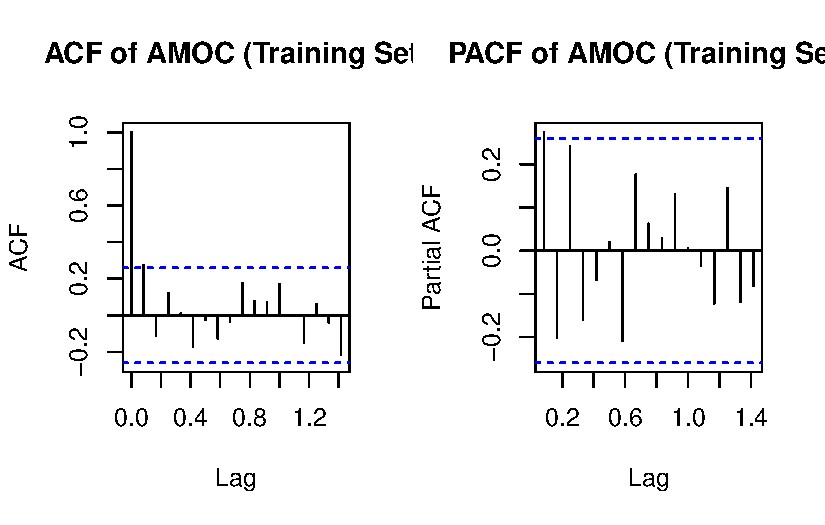
\includegraphics{project_files/figure-pdf/fig-AMF+PACF-1.pdf}

}

\caption{ACF and PACF of Monthly AMOC}

\end{figure}%

\begin{Shaded}
\begin{Highlighting}[]
\FunctionTok{par}\NormalTok{(}\AttributeTok{mfrow =} \FunctionTok{c}\NormalTok{(}\DecValTok{1}\NormalTok{, }\DecValTok{1}\NormalTok{))}
\end{Highlighting}
\end{Shaded}

The ACF exhibits a strong lag-1 autocorrelation and a slow decay,
consistent with a non-stationary process. The PACF shows a clear spike
at lag 1 and minimal structure thereafter, suggesting that differencing
followed by a low-order AR term may capture the residual dynamics ---
motivating the selection of ARIMA(1,1,0) and ARIMA(1,1,1) candidates.

\paragraph{Transforming for
Stationarity}\label{transforming-for-stationarity}

\begin{Shaded}
\begin{Highlighting}[]
\CommentTok{\# First{-}order differencing}
\NormalTok{diff\_amoc }\OtherTok{\textless{}{-}} \FunctionTok{diff}\NormalTok{(train\_ts)}

\CommentTok{\# Plot layout: 1 row, 3 plots}
\FunctionTok{par}\NormalTok{(}\AttributeTok{mfrow =} \FunctionTok{c}\NormalTok{(}\DecValTok{1}\NormalTok{, }\DecValTok{3}\NormalTok{), }\AttributeTok{mar =} \FunctionTok{c}\NormalTok{(}\DecValTok{4}\NormalTok{, }\DecValTok{4}\NormalTok{, }\FloatTok{3.5}\NormalTok{, }\DecValTok{1}\NormalTok{))}

\CommentTok{\# Plot 1: Differenced Series}
\FunctionTok{plot}\NormalTok{(diff\_amoc, }
     \AttributeTok{main =} \StringTok{"First{-}order Differenced AMOC"}\NormalTok{, }
     \AttributeTok{ylab =} \StringTok{"Differenced Value"}\NormalTok{, }
     \AttributeTok{xlab =} \StringTok{"Time"}\NormalTok{, }
     \AttributeTok{col =} \StringTok{"steelblue"}\NormalTok{, }
     \AttributeTok{lwd =} \FloatTok{1.2}\NormalTok{)}

\CommentTok{\# Plot 2: ACF}
\FunctionTok{acf}\NormalTok{(diff\_amoc, }
    \AttributeTok{main =} \StringTok{"ACF of Differenced Series"}\NormalTok{, }
    \AttributeTok{col =} \StringTok{"black"}\NormalTok{)}

\CommentTok{\# Plot 3: PACF}
\FunctionTok{pacf}\NormalTok{(diff\_amoc, }
     \AttributeTok{main =} \StringTok{"PACF of Differenced Series"}\NormalTok{, }
     \AttributeTok{col =} \StringTok{"black"}\NormalTok{)}
\end{Highlighting}
\end{Shaded}

\begin{figure}[H]

{\centering 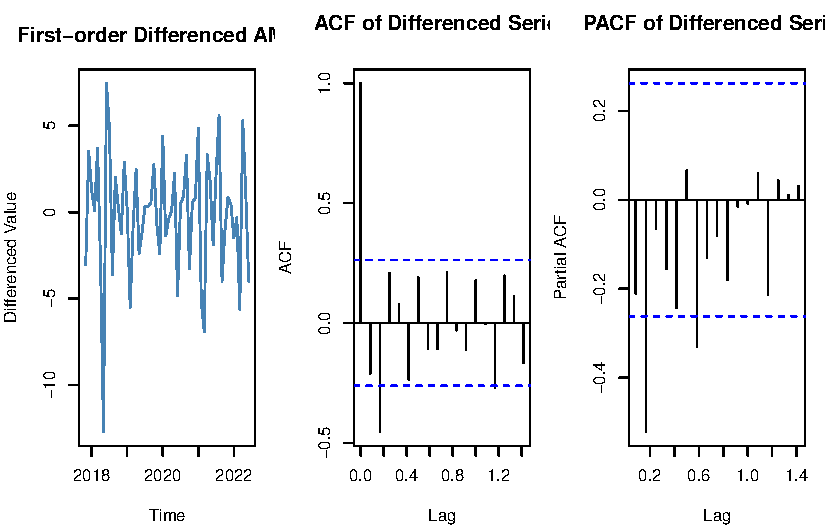
\includegraphics{project_files/figure-pdf/fig-diff-acf-pacf-1.pdf}

}

\caption{ARIMA differencing ACF/PACF}

\end{figure}%

\textbf{Figure 15} shows the first-order differenced AMOC series and its
autocorrelation diagnostics. The differenced series now fluctuates
around a constant mean, with no evident trend, indicating that
\textbf{stationarity has been successfully induced}.

The \textbf{ACF} decays rapidly, with most lags falling within the 95\%
confidence bounds after lag 1 --- a strong sign that the
\textbf{stochastic trend has been removed}. The \textbf{PACF} shows a
single large spike at lag 1, suggesting the presence of \textbf{short
memory dependence}, likely capturable with a \textbf{low-order AR or MA
term}.

These patterns collectively support the use of
\textbf{ARIMA(}\(p\)\textbf{,1,}\(q\)\textbf{)} models with
\textbf{first-order differencing} to address non-stationarity, and
\textbf{either} \(p=1\) \textbf{or} \(q=1\) to reflect the short memory
structure.

\paragraph{Model Rationale and Modelling
Strategy}\label{model-rationale-and-modelling-strategy}

To model the temporal dynamics of the Atlantic Meridional Overturning
Circulation (AMOC), we consider both \textbf{ARMA} and \textbf{ARIMA}
models --- linear time series models commonly applied in climatological
and environmental research to capture autocorrelation and generate
forecasts.

Initial inspection of the raw series revealed \textbf{non-stationarity},
with strong autocorrelation at lag 1 and slow ACF decay. After applying
\textbf{first-order differencing}, the series showed visual
stationarity, and its ACF and PACF indicated \textbf{short memory
structure}: a moderate lag-1 autocorrelation and a large negative spike
in PACF at lag 1. These patterns support the use of
\textbf{ARIMA(}\(p\)\textbf{,1,}\(q\)\textbf{)} models, where \(d=1\)
accounts for stochastic trend, and \(p\) or \(q\) captures the
short-term dependence.

We adopt a two-pronged modelling strategy:

\begin{itemize}
\item
  \textbf{ARMA models} on the undifferenced series serve as a benchmark,
  capturing autocorrelation in the original (non-stationary) data.
\item
  \textbf{ARIMA models} on the differenced series address the identified
  non-stationarity more explicitly.
\end{itemize}

Based on the ACF/PACF structure and model parsimony, we examine the
following candidates:

\begin{itemize}
\item
  \textbf{ARMA(1,0)} and \textbf{ARMA(2,0)}: simple autoregressive
  models without differencing.
\item
  \textbf{ARIMA(1,1,0)}, \textbf{ARIMA(0,1,1)}, and
  \textbf{ARIMA(1,1,1)}: models with first-order differencing and
  varying AR/MA terms.
\end{itemize}

All models are estimated using \textbf{maximum likelihood} via R's
\texttt{arima()} function and evaluated based on:

\begin{itemize}
\item
  \textbf{Akaike Information Criterion (AIC)}
\item
  \textbf{Residual diagnostics} (ACF, Q--Q plots, visual residuals
\item
  \textbf{Ljung--Box tests} for autocorrelation
\item
  And ultimately, \textbf{forecast performance on the 8-month test set
  (July 2022 -- February 2023)}
\end{itemize}

This modelling strategy balances \textbf{diagnostic rigour},
\textbf{parsimony}, and \textbf{forecast relevance}, ensuring that model
selection is both statistically defensible and practically informed.

\paragraph{ARMA Model Fitting (Undifferenced
Series)}\label{arma-model-fitting-undifferenced-series}

We first fit two ARMA models to the undifferenced AMOC series for
benchmarking. The \textbf{ARMA(1,0)} model estimated:

\[
X_t = 16.88 + 0.28 X_{t-1} + \varepsilon_t, \quad \varepsilon_t \sim \mathcal{N}(0, \sigma^2)
\] The \textbf{ARMA(2,0)} model extended this with a second lag: \[
X_t = 16.90 + 0.34 X_{t-1} - 0.21 X_{t-2} + \varepsilon_t, \quad \varepsilon_t \sim \mathcal{N}(0, \sigma^2)
\]

\begin{Shaded}
\begin{Highlighting}[]
\CommentTok{\# ARMA Models}
\NormalTok{arma\_10 }\OtherTok{\textless{}{-}} \FunctionTok{arima}\NormalTok{(train\_ts, }\AttributeTok{order =} \FunctionTok{c}\NormalTok{(}\DecValTok{1}\NormalTok{,}\DecValTok{0}\NormalTok{,}\DecValTok{0}\NormalTok{), }\AttributeTok{method =} \StringTok{"ML"}\NormalTok{)}
\NormalTok{arma\_20 }\OtherTok{\textless{}{-}} \FunctionTok{arima}\NormalTok{(train\_ts, }\AttributeTok{order =} \FunctionTok{c}\NormalTok{(}\DecValTok{2}\NormalTok{,}\DecValTok{0}\NormalTok{,}\DecValTok{0}\NormalTok{), }\AttributeTok{method =} \StringTok{"ML"}\NormalTok{)}
\end{Highlighting}
\end{Shaded}

\begin{Shaded}
\begin{Highlighting}[]
\FunctionTok{par}\NormalTok{(}\AttributeTok{mfrow =} \FunctionTok{c}\NormalTok{(}\DecValTok{2}\NormalTok{,}\DecValTok{3}\NormalTok{), }\AttributeTok{mar =} \FunctionTok{c}\NormalTok{(}\DecValTok{4}\NormalTok{,}\DecValTok{4}\NormalTok{,}\DecValTok{2}\NormalTok{,}\DecValTok{1}\NormalTok{))}
\FunctionTok{plot}\NormalTok{(}\FunctionTok{residuals}\NormalTok{(arma\_10), }\AttributeTok{main =} \StringTok{"ARMA(1,0) Residuals"}\NormalTok{)}
\FunctionTok{acf}\NormalTok{(}\FunctionTok{residuals}\NormalTok{(arma\_10), }\AttributeTok{main =} \StringTok{"ARMA(1,0) ACF"}\NormalTok{)}
\FunctionTok{qqnorm}\NormalTok{(}\FunctionTok{residuals}\NormalTok{(arma\_10)); }\FunctionTok{qqline}\NormalTok{(}\FunctionTok{residuals}\NormalTok{(arma\_10))}

\FunctionTok{plot}\NormalTok{(}\FunctionTok{residuals}\NormalTok{(arma\_20), }\AttributeTok{main =} \StringTok{"ARMA(2,0) Residuals"}\NormalTok{)}
\FunctionTok{acf}\NormalTok{(}\FunctionTok{residuals}\NormalTok{(arma\_20), }\AttributeTok{main =} \StringTok{"ARMA(2,0) ACF"}\NormalTok{)}
\FunctionTok{qqnorm}\NormalTok{(}\FunctionTok{residuals}\NormalTok{(arma\_20)); }\FunctionTok{qqline}\NormalTok{(}\FunctionTok{residuals}\NormalTok{(arma\_20))}
\end{Highlighting}
\end{Shaded}

\begin{figure}[H]

{\centering 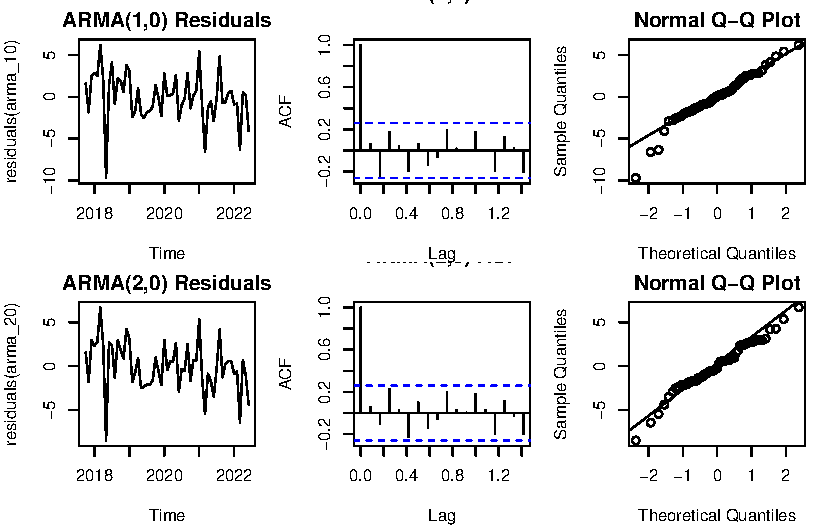
\includegraphics{project_files/figure-pdf/fig-arma-diagnostics-1.pdf}

}

\caption{Residual Diagnostics for ARMA(1,0) and ARMA(2,0)}

\end{figure}%

\begin{Shaded}
\begin{Highlighting}[]
\FunctionTok{par}\NormalTok{(}\AttributeTok{mfrow =} \FunctionTok{c}\NormalTok{(}\DecValTok{1}\NormalTok{,}\DecValTok{1}\NormalTok{))}
\end{Highlighting}
\end{Shaded}

\paragraph{Model Comparison}\label{model-comparison}

\begin{longtable}[]{@{}
  >{\raggedright\arraybackslash}p{(\columnwidth - 8\tabcolsep) * \real{0.2000}}
  >{\raggedright\arraybackslash}p{(\columnwidth - 8\tabcolsep) * \real{0.2000}}
  >{\raggedright\arraybackslash}p{(\columnwidth - 8\tabcolsep) * \real{0.2000}}
  >{\raggedright\arraybackslash}p{(\columnwidth - 8\tabcolsep) * \real{0.2000}}
  >{\raggedright\arraybackslash}p{(\columnwidth - 8\tabcolsep) * \real{0.2000}}@{}}
\toprule\noalign{}
\begin{minipage}[b]{\linewidth}\raggedright
Model
\end{minipage} & \begin{minipage}[b]{\linewidth}\raggedright
AIC
\end{minipage} & \begin{minipage}[b]{\linewidth}\raggedright
AR Coefficients
\end{minipage} & \begin{minipage}[b]{\linewidth}\raggedright
Ljung--Box p-value
\end{minipage} & \begin{minipage}[b]{\linewidth}\raggedright
Residual Summary
\end{minipage} \\
\midrule\noalign{}
\endhead
\bottomrule\noalign{}
\endlastfoot
ARMA(1,0) & 286.18 & AR(1) = 0.2807 & \textgreater{} 0.24 & Some
residual autocorrelation \\
ARMA(2,0) & 285.65 & AR(1) = 0.342, AR(2) = -0.209 & 0.26 & Slightly
improved white noise \\
\end{longtable}

The \textbf{ARMA(1,0)} model yielded an AIC of \textbf{286.18}.
Residuals appear mean-centred and approximately homoscedastic, though
the \textbf{ACF shows mild low-lag autocorrelation}, consistent with an
underfitted model. The Q--Q plot indicates reasonably normal residuals
with only slight tail deviations.

The \textbf{ARMA(2,0)} model provided a \textbf{marginal AIC improvement
to 285.65}. The residual ACF falls entirely within the 95\% bounds,
suggesting reduced autocorrelation. However, the Q--Q plot shows
\textbf{slightly heavier left-tail deviation}, with residuals straying
from normality more than in the ARMA(1,0) case. The \textbf{Ljung--Box
p-value increased to 0.26}, further supporting weaker residual
dependence.

Although ARMA(2,0) shows statistical improvement in AIC and whiteness,
\textbf{its residual distribution is slightly less normal}, and both
models remain limited by the assumption of stationarity. This, combined
with the underlying stochastic trend in the original series, justifies
moving forward with differenced models --- namely \textbf{ARIMA}.

\paragraph{ARIMA Model Fitting (Differenced
Series)}\label{arima-model-fitting-differenced-series}

\begin{Shaded}
\begin{Highlighting}[]
\NormalTok{arima\_110 }\OtherTok{\textless{}{-}} \FunctionTok{arima}\NormalTok{(train\_ts, }\AttributeTok{order =} \FunctionTok{c}\NormalTok{(}\DecValTok{1}\NormalTok{,}\DecValTok{1}\NormalTok{,}\DecValTok{0}\NormalTok{), }\AttributeTok{method =} \StringTok{"ML"}\NormalTok{)}
\NormalTok{arima\_011 }\OtherTok{\textless{}{-}} \FunctionTok{arima}\NormalTok{(train\_ts, }\AttributeTok{order =} \FunctionTok{c}\NormalTok{(}\DecValTok{0}\NormalTok{,}\DecValTok{1}\NormalTok{,}\DecValTok{1}\NormalTok{), }\AttributeTok{method =} \StringTok{"ML"}\NormalTok{)}
\NormalTok{arima\_111 }\OtherTok{\textless{}{-}} \FunctionTok{arima}\NormalTok{(train\_ts, }\AttributeTok{order =} \FunctionTok{c}\NormalTok{(}\DecValTok{1}\NormalTok{,}\DecValTok{1}\NormalTok{,}\DecValTok{1}\NormalTok{), }\AttributeTok{method =} \StringTok{"ML"}\NormalTok{)}
\end{Highlighting}
\end{Shaded}

\begin{Shaded}
\begin{Highlighting}[]
\CommentTok{\# Diagnostic plotting function}
\NormalTok{plot\_diagnostics }\OtherTok{\textless{}{-}} \ControlFlowTok{function}\NormalTok{(model, model\_name, col\_line) \{}
  \FunctionTok{layout}\NormalTok{(}\FunctionTok{matrix}\NormalTok{(}\DecValTok{1}\SpecialCharTok{:}\DecValTok{3}\NormalTok{, }\DecValTok{1}\NormalTok{, }\DecValTok{3}\NormalTok{, }\AttributeTok{byrow =} \ConstantTok{TRUE}\NormalTok{), }\AttributeTok{widths =} \FunctionTok{c}\NormalTok{(}\FloatTok{1.4}\NormalTok{, }\DecValTok{1}\NormalTok{, }\DecValTok{1}\NormalTok{))}
  \FunctionTok{par}\NormalTok{(}\AttributeTok{mar =} \FunctionTok{c}\NormalTok{(}\DecValTok{4}\NormalTok{, }\DecValTok{4}\NormalTok{, }\DecValTok{3}\NormalTok{, }\DecValTok{1}\NormalTok{))}
  
  \FunctionTok{plot}\NormalTok{(}\FunctionTok{residuals}\NormalTok{(model), }\AttributeTok{type =} \StringTok{"l"}\NormalTok{, }\AttributeTok{col =}\NormalTok{ col\_line, }\AttributeTok{lwd =} \FloatTok{1.2}\NormalTok{,}
       \AttributeTok{main =} \FunctionTok{paste}\NormalTok{(model\_name, }\StringTok{"Residuals"}\NormalTok{), }\AttributeTok{ylab =} \StringTok{"Residuals"}\NormalTok{, }\AttributeTok{xlab =} \StringTok{"Time"}\NormalTok{)}
  \FunctionTok{acf}\NormalTok{(}\FunctionTok{residuals}\NormalTok{(model), }\AttributeTok{main =} \StringTok{"ACF of Residuals"}\NormalTok{, }\AttributeTok{col =} \StringTok{"black"}\NormalTok{, }\AttributeTok{lwd =} \FloatTok{1.2}\NormalTok{)}
  \FunctionTok{qqnorm}\NormalTok{(}\FunctionTok{residuals}\NormalTok{(model), }\AttributeTok{main =} \StringTok{"Normal Q–Q Plot"}\NormalTok{)}
  \FunctionTok{qqline}\NormalTok{(}\FunctionTok{residuals}\NormalTok{(model), }\AttributeTok{col =} \StringTok{"red"}\NormalTok{, }\AttributeTok{lwd =} \FloatTok{1.2}\NormalTok{)}
  
  \FunctionTok{layout}\NormalTok{(}\DecValTok{1}\NormalTok{)}
\NormalTok{\}}

\FunctionTok{plot\_diagnostics}\NormalTok{(arima\_110, }\StringTok{"ARIMA(1,1,0)"}\NormalTok{, }\StringTok{"steelblue"}\NormalTok{)}
\end{Highlighting}
\end{Shaded}

\begin{figure}[H]

{\centering 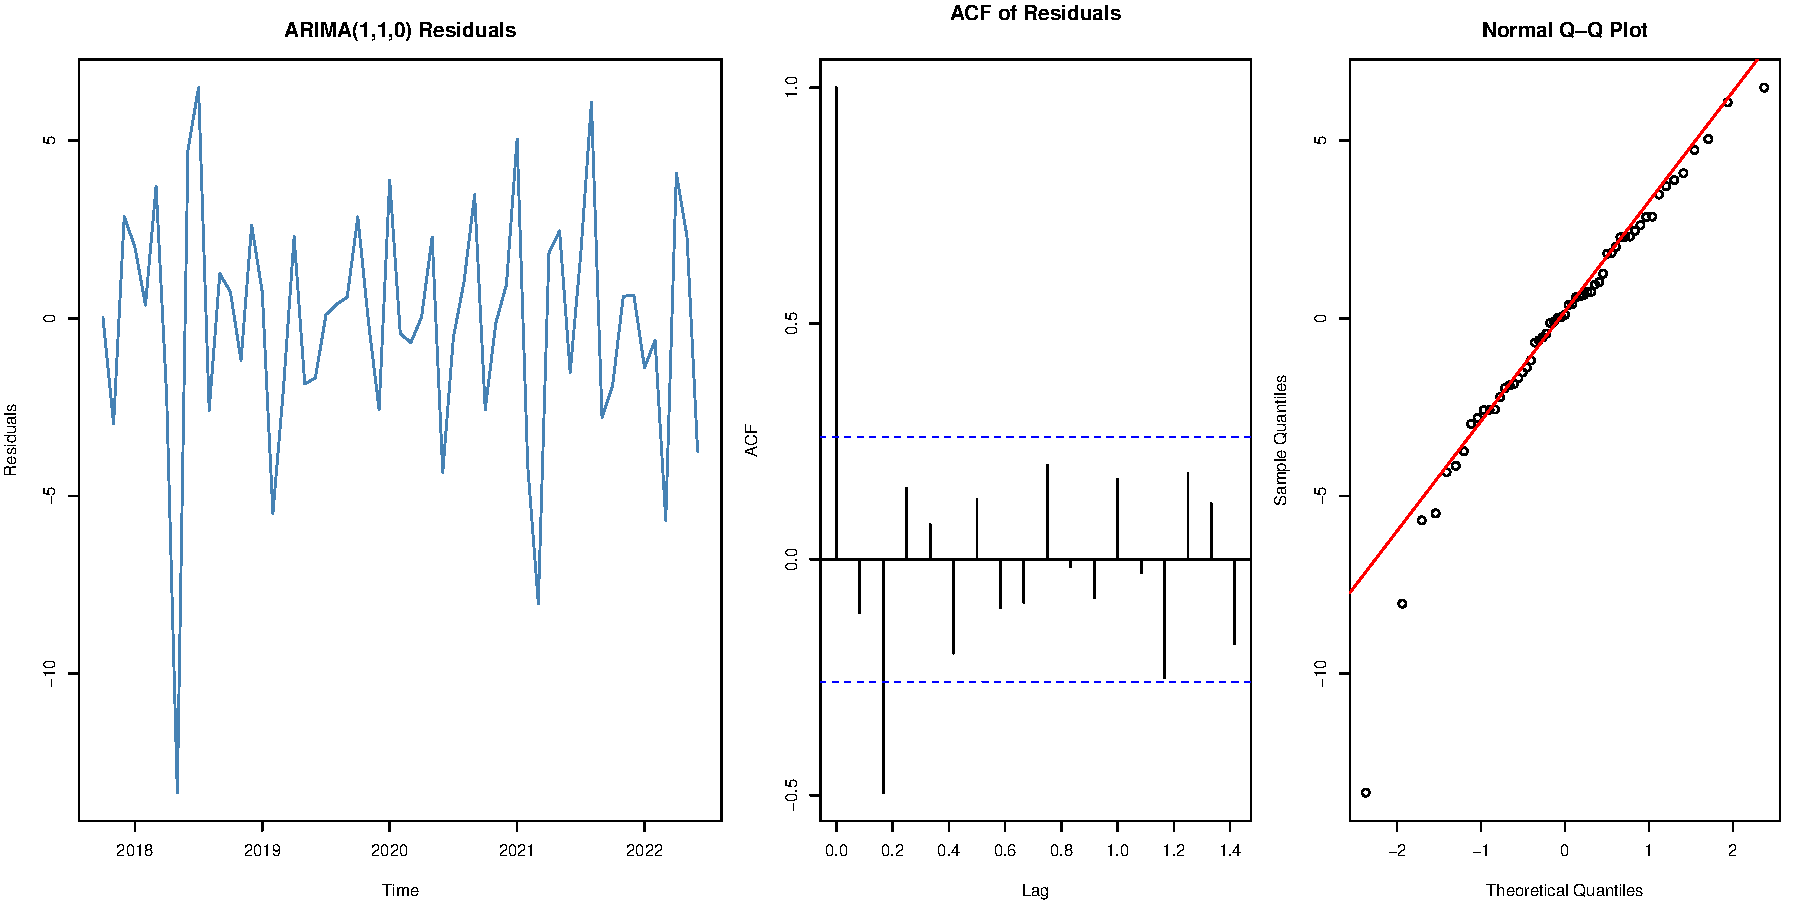
\includegraphics{project_files/figure-pdf/fig-arima-diagnostics-1.pdf}

}

\caption{Residual diagnostics for candidate ARIMA models}

\end{figure}%

\begin{Shaded}
\begin{Highlighting}[]
\FunctionTok{plot\_diagnostics}\NormalTok{(arima\_011, }\StringTok{"ARIMA(0,1,1)"}\NormalTok{, }\StringTok{"darkred"}\NormalTok{)}
\end{Highlighting}
\end{Shaded}

\begin{figure}[H]

{\centering 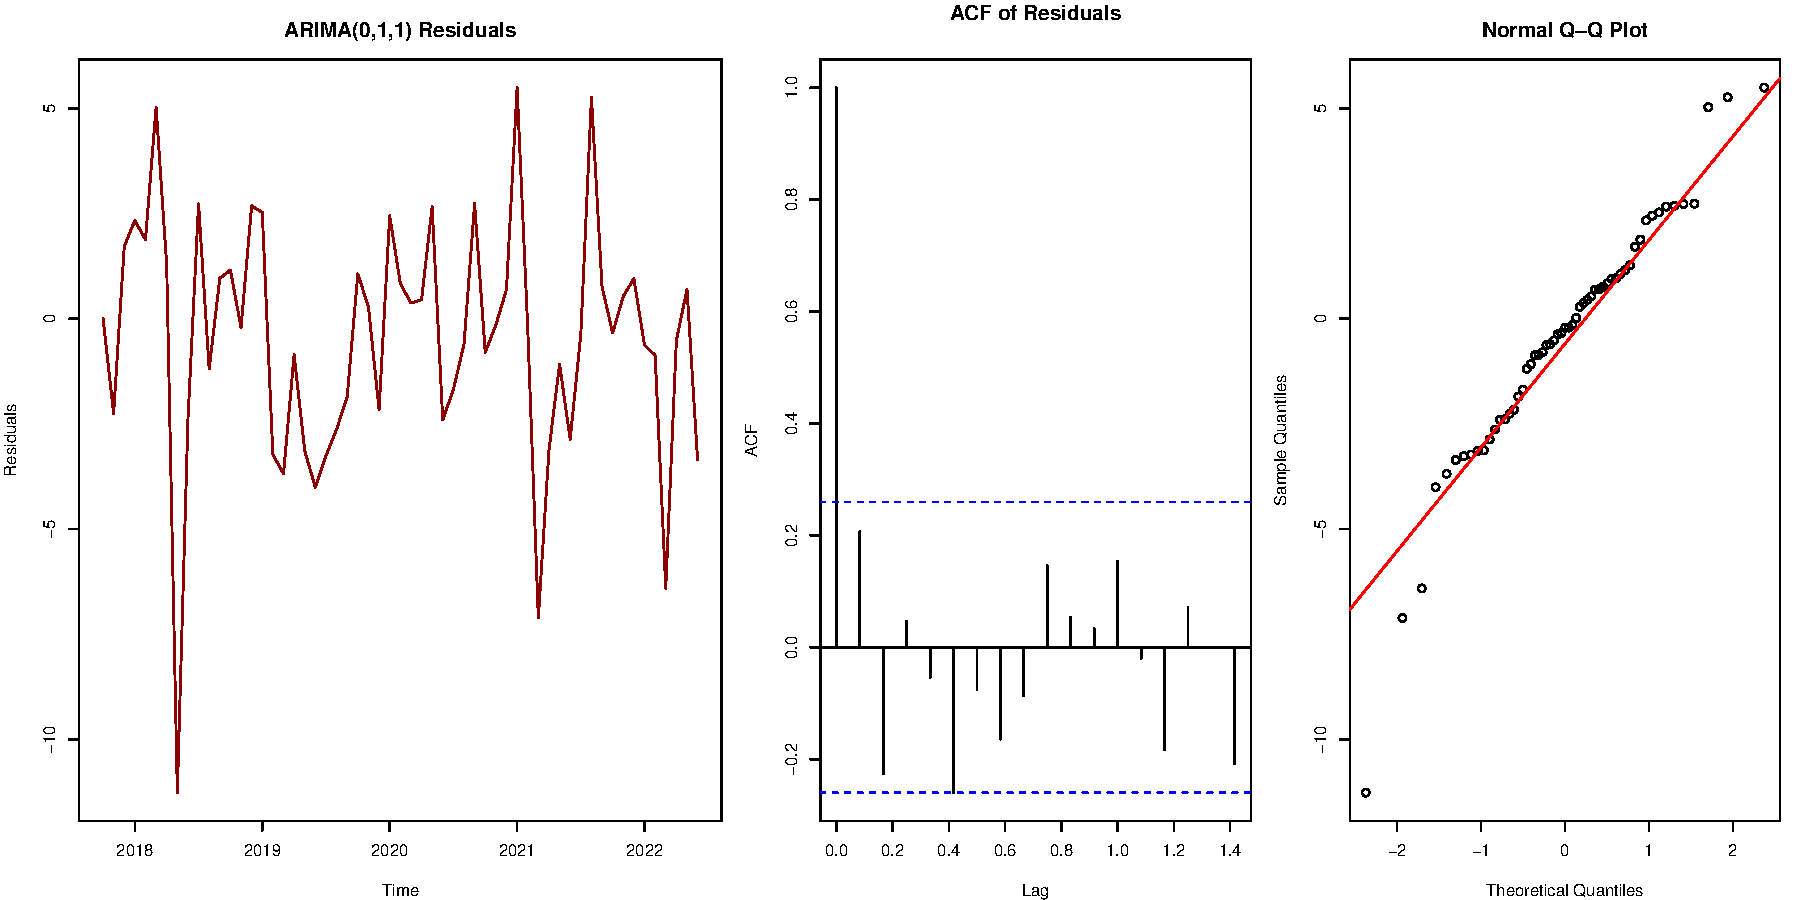
\includegraphics{project_files/figure-pdf/fig-arima-diagnostics-2.pdf}

}

\caption{Residual diagnostics for candidate ARIMA models}

\end{figure}%

\begin{Shaded}
\begin{Highlighting}[]
\FunctionTok{plot\_diagnostics}\NormalTok{(arima\_111, }\StringTok{"ARIMA(1,1,1)"}\NormalTok{, }\StringTok{"darkgreen"}\NormalTok{)}
\end{Highlighting}
\end{Shaded}

\begin{figure}[H]

{\centering 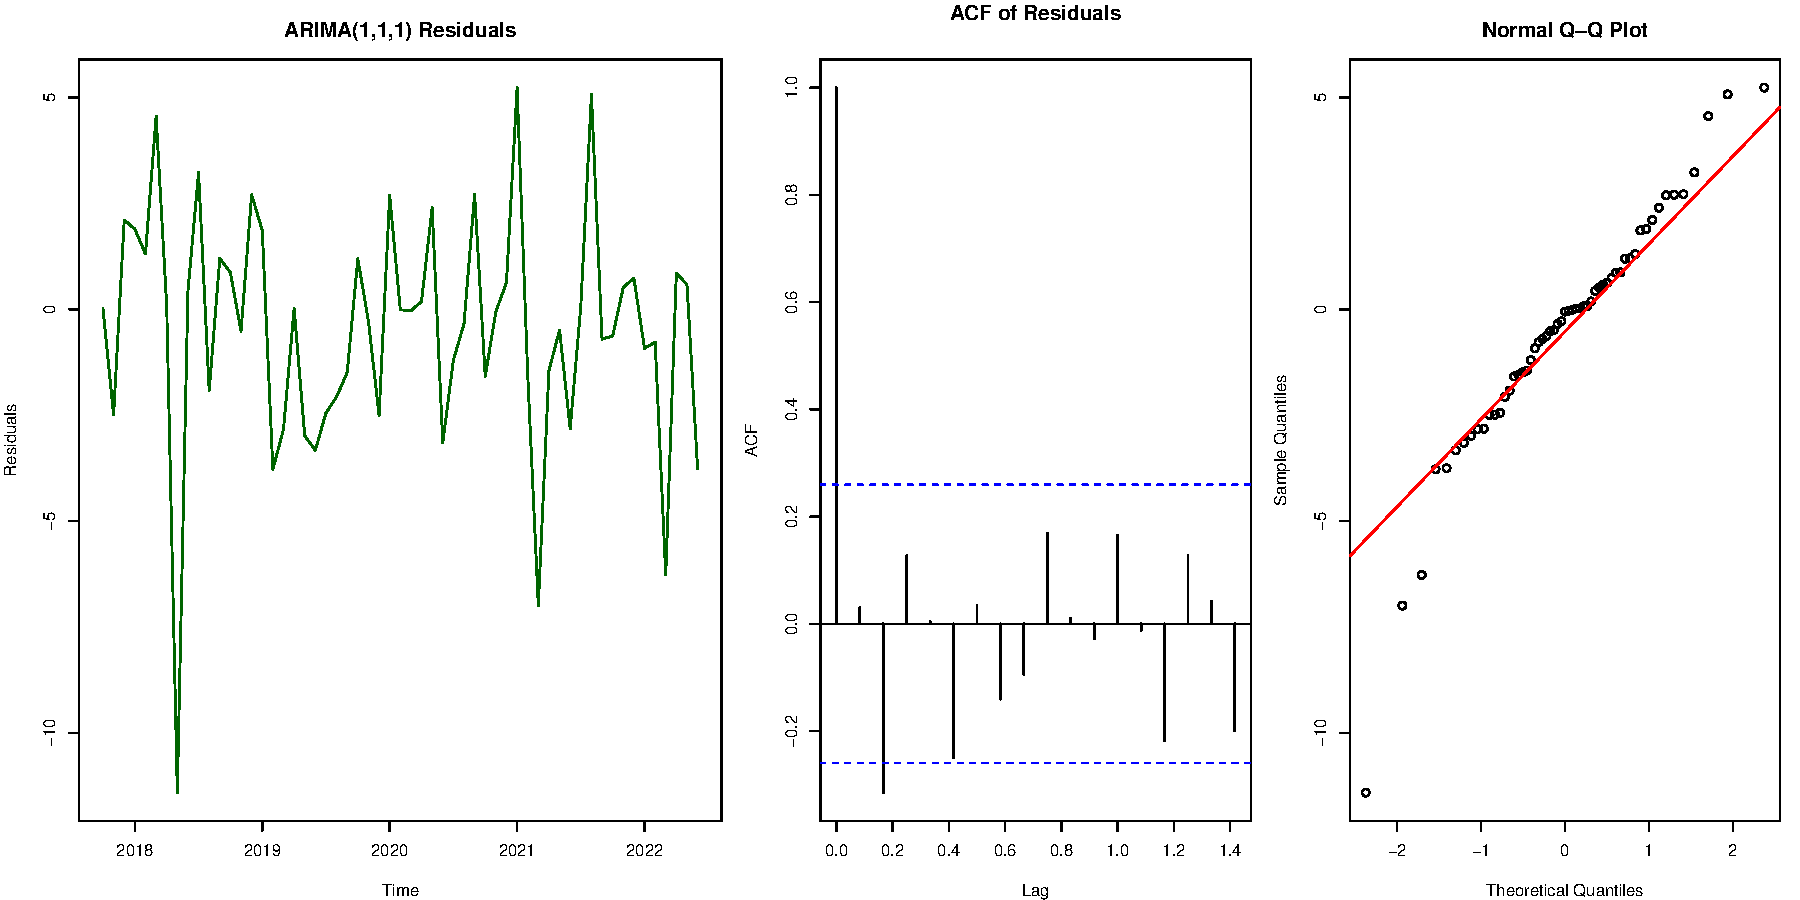
\includegraphics{project_files/figure-pdf/fig-arima-diagnostics-3.pdf}

}

\caption{Residual diagnostics for candidate ARIMA models}

\end{figure}%

\begin{Shaded}
\begin{Highlighting}[]
\CommentTok{\# Ljung–Box Tests}
\NormalTok{lb\_110 }\OtherTok{\textless{}{-}} \FunctionTok{Box.test}\NormalTok{(}\FunctionTok{residuals}\NormalTok{(arima\_110), }\AttributeTok{lag =} \DecValTok{10}\NormalTok{, }\AttributeTok{type =} \StringTok{"Ljung{-}Box"}\NormalTok{)}
\NormalTok{lb\_011 }\OtherTok{\textless{}{-}} \FunctionTok{Box.test}\NormalTok{(}\FunctionTok{residuals}\NormalTok{(arima\_011), }\AttributeTok{lag =} \DecValTok{10}\NormalTok{, }\AttributeTok{type =} \StringTok{"Ljung{-}Box"}\NormalTok{)}
\NormalTok{lb\_111 }\OtherTok{\textless{}{-}} \FunctionTok{Box.test}\NormalTok{(}\FunctionTok{residuals}\NormalTok{(arima\_111), }\AttributeTok{lag =} \DecValTok{10}\NormalTok{, }\AttributeTok{type =} \StringTok{"Ljung{-}Box"}\NormalTok{)}

\NormalTok{knitr}\SpecialCharTok{::}\FunctionTok{kable}\NormalTok{(}\FunctionTok{data.frame}\NormalTok{(}
  \AttributeTok{Model =} \FunctionTok{c}\NormalTok{(}\StringTok{"ARIMA(1,1,0)"}\NormalTok{, }\StringTok{"ARIMA(0,1,1)"}\NormalTok{, }\StringTok{"ARIMA(1,1,1)"}\NormalTok{),}
  \AttributeTok{AIC =} \FunctionTok{c}\NormalTok{(}\FunctionTok{AIC}\NormalTok{(arima\_110), }\FunctionTok{AIC}\NormalTok{(arima\_011), }\FunctionTok{AIC}\NormalTok{(arima\_111)),}
  \AttributeTok{Ljung\_Box\_p =} \FunctionTok{c}\NormalTok{(lb\_110}\SpecialCharTok{$}\NormalTok{p.value, lb\_011}\SpecialCharTok{$}\NormalTok{p.value, lb\_111}\SpecialCharTok{$}\NormalTok{p.value),}
  \AttributeTok{Notes =} \FunctionTok{c}\NormalTok{(}\StringTok{"Residual autocorr."}\NormalTok{, }\StringTok{"Good fit"}\NormalTok{, }\StringTok{"Best fit"}\NormalTok{)}
\NormalTok{), }\AttributeTok{caption =} \StringTok{"Comparison of ARIMA Models"}\NormalTok{)}
\end{Highlighting}
\end{Shaded}

\begin{longtable}[]{@{}lrrl@{}}
\caption{Comparison of ARIMA Models}\tabularnewline
\toprule\noalign{}
Model & AIC & Ljung\_Box\_p & Notes \\
\midrule\noalign{}
\endfirsthead
\toprule\noalign{}
Model & AIC & Ljung\_Box\_p & Notes \\
\midrule\noalign{}
\endhead
\bottomrule\noalign{}
\endlastfoot
ARIMA(1,1,0) & 301.4389 & 0.0050499 & Residual autocorr. \\
ARIMA(0,1,1) & 286.6222 & 0.1412433 & Good fit \\
ARIMA(1,1,1) & 285.0751 & 0.1265184 & Best fit \\
\end{longtable}

\paragraph{Findings}\label{findings}

The three ARIMA models were evaluated using AIC, residual
autocorrelation (via ACF and Ljung--Box test), and normality (via Q--Q
plots).

\begin{itemize}
\item
  The \textbf{ARIMA(1,1,0)} model performed poorly. It yielded an AIC of
  \textbf{301.4}, and its residuals displayed \textbf{significant
  autocorrelation} (Ljung--Box p = \textbf{0.005}) and noticeable
  non-normality in the left tail of the Q--Q plot. These features
  indicate an underfitted model that fails to adequately capture the
  series dynamics.
\item
  In contrast, the \textbf{ARIMA(0,1,1)} model achieved a substantial
  improvement, reducing AIC to \textbf{286.6}, and removing most
  autocorrelation (Ljung--Box p = \textbf{0.14}). The residuals were
  stable, and the Q--Q plot showed only slight tail curvature,
  indicating a much better overall fit.
\item
  The \textbf{ARIMA(1,1,1)} model yielded the \textbf{lowest AIC
  (285.1)} and the best residual diagnostics. Its residual ACF showed no
  significant autocorrelation (Ljung--Box p = \textbf{0.13}), and the
  Q--Q plot followed the 1:1 line closely. This model effectively
  balances goodness-of-fit with simplicity and is therefore selected as
  the \textbf{benchmark model}.
\end{itemize}

\paragraph{Model Refinement and
Justification}\label{model-refinement-and-justification}

Although ARIMA(1,1,1) performs well, \textbf{minor residual
autocorrelation} and slight non-normality remain. To assess whether
these artefacts reflect underfitting, we explore two higher-order
models: \textbf{ARIMA(2,1,0)} and \textbf{ARIMA(2,1,2)}.

This refinement is motivated by:

\begin{itemize}
\item
  \textbf{Persistent low-lag structure} in the differenced ACF/PACF
  plots
\item
  The potential for \textbf{medium-term dependence} not captured by
  first-order terms
\item
  Precedent from similar climatological time series, where
  \textbf{ARIMA(2,1,2)} often improves predictive performance.
\end{itemize}

\begin{Shaded}
\begin{Highlighting}[]
\NormalTok{arima\_210 }\OtherTok{\textless{}{-}} \FunctionTok{arima}\NormalTok{(train\_ts, }\AttributeTok{order =} \FunctionTok{c}\NormalTok{(}\DecValTok{2}\NormalTok{,}\DecValTok{1}\NormalTok{,}\DecValTok{0}\NormalTok{), }\AttributeTok{method =} \StringTok{"ML"}\NormalTok{)}
\NormalTok{arima\_212 }\OtherTok{\textless{}{-}} \FunctionTok{arima}\NormalTok{(train\_ts, }\AttributeTok{order =} \FunctionTok{c}\NormalTok{(}\DecValTok{2}\NormalTok{,}\DecValTok{1}\NormalTok{,}\DecValTok{2}\NormalTok{), }\AttributeTok{method =} \StringTok{"ML"}\NormalTok{)}

\NormalTok{lb\_210 }\OtherTok{\textless{}{-}} \FunctionTok{Box.test}\NormalTok{(}\FunctionTok{residuals}\NormalTok{(arima\_210), }\AttributeTok{lag =} \DecValTok{10}\NormalTok{, }\AttributeTok{type =} \StringTok{"Ljung{-}Box"}\NormalTok{)}
\NormalTok{lb\_212 }\OtherTok{\textless{}{-}} \FunctionTok{Box.test}\NormalTok{(}\FunctionTok{residuals}\NormalTok{(arima\_212), }\AttributeTok{lag =} \DecValTok{10}\NormalTok{, }\AttributeTok{type =} \StringTok{"Ljung{-}Box"}\NormalTok{)}
\end{Highlighting}
\end{Shaded}

\begin{Shaded}
\begin{Highlighting}[]
\NormalTok{knitr}\SpecialCharTok{::}\FunctionTok{kable}\NormalTok{(}\FunctionTok{data.frame}\NormalTok{(}
  \AttributeTok{Model =} \FunctionTok{c}\NormalTok{(}\StringTok{"ARIMA(2,1,0)"}\NormalTok{, }\StringTok{"ARIMA(2,1,2)"}\NormalTok{),}
  \AttributeTok{AIC =} \FunctionTok{c}\NormalTok{(}\FunctionTok{AIC}\NormalTok{(arima\_210), }\FunctionTok{AIC}\NormalTok{(arima\_212)),}
  \AttributeTok{Ljung\_Box\_p =} \FunctionTok{c}\NormalTok{(lb\_210}\SpecialCharTok{$}\NormalTok{p.value, lb\_212}\SpecialCharTok{$}\NormalTok{p.value),}
  \AttributeTok{Notes =} \FunctionTok{c}\NormalTok{(}\StringTok{"No clear improvement"}\NormalTok{, }\StringTok{"Slight AIC gain, more complex"}\NormalTok{)}
\NormalTok{), }\AttributeTok{caption =} \StringTok{"Refined ARIMA Models"}\NormalTok{)}
\end{Highlighting}
\end{Shaded}

\begin{longtable}[]{@{}lrrl@{}}
\caption{Refined ARIMA Models}\tabularnewline
\toprule\noalign{}
Model & AIC & Ljung\_Box\_p & Notes \\
\midrule\noalign{}
\endfirsthead
\toprule\noalign{}
Model & AIC & Ljung\_Box\_p & Notes \\
\midrule\noalign{}
\endhead
\bottomrule\noalign{}
\endlastfoot
ARIMA(2,1,0) & 285.5323 & 0.3362862 & No clear improvement \\
ARIMA(2,1,2) & 282.7781 & 0.3303888 & Slight AIC gain, more complex \\
\end{longtable}

As shown in \textbf{Table 12}, \textbf{ARIMA(2,1,2)} achieved a modest
reduction in AIC compared to ARIMA(1,1,1), and both refined models
returned Ljung--Box p-values above 0.3, suggesting no significant
autocorrelation in the residuals.

While ARIMA(2,1,2) performs best by AIC, the improvement over
ARIMA(1,1,1) is \textbf{minor}, and comes at the cost of a \textbf{more
complex structure}. Given the principle of model parsimony, and the lack
of clear diagnostic benefit, \textbf{ARIMA(1,1,1)} is retained as the
preferred model.

Through ACF/PACF analysis and iterative model fitting, we identified
ARIMA(1,1,1) as the most appropriate model for the monthly AMOC series.
While higher-order alternatives offered marginal AIC improvements,
residual diagnostics and parsimony considerations supported retention of
ARIMA(1,1,1).

\subsection{Part C: Quarterly Modelling of
AMOC}\label{part-c-quarterly-modelling-of-amoc}

To explore lower-frequency dynamics in the AMOC time series, the data is
aggregated from monthly to quarterly averages. This aligns with
climatological practice where quarterly data can help reveal medium-term
structure by smoothing high-frequency noise.

\begin{Shaded}
\begin{Highlighting}[]
\FunctionTok{library}\NormalTok{(dplyr)}
\FunctionTok{library}\NormalTok{(zoo)}

\NormalTok{moc\_df\_q }\OtherTok{\textless{}{-}}\NormalTok{ moc\_df }\SpecialCharTok{\%\textgreater{}\%}
  \FunctionTok{mutate}\NormalTok{(}\AttributeTok{quarter =} \FunctionTok{as.yearqtr}\NormalTok{(date)) }\SpecialCharTok{\%\textgreater{}\%}
  \FunctionTok{group\_by}\NormalTok{(quarter) }\SpecialCharTok{\%\textgreater{}\%}
  \FunctionTok{summarise}\NormalTok{(}\AttributeTok{amoc\_q =} \FunctionTok{mean}\NormalTok{(amoc, }\AttributeTok{na.rm =} \ConstantTok{TRUE}\NormalTok{)) }\SpecialCharTok{\%\textgreater{}\%}
  \FunctionTok{ungroup}\NormalTok{()}
\end{Highlighting}
\end{Shaded}

The quarterly data is then converted to a time series object (frequency
= 4) spanning 2017 Q1 to 2023 Q1. The final two quarters are withheld
for out-of-sample forecast validation.

\begin{Shaded}
\begin{Highlighting}[]
\CommentTok{\# Create quarterly time series}
\NormalTok{amoc\_q\_ts }\OtherTok{\textless{}{-}} \FunctionTok{ts}\NormalTok{(moc\_df\_q}\SpecialCharTok{$}\NormalTok{amoc\_q, }\AttributeTok{start =} \FunctionTok{c}\NormalTok{(}\DecValTok{2017}\NormalTok{, }\DecValTok{3}\NormalTok{), }\AttributeTok{frequency =} \DecValTok{4}\NormalTok{)}

\CommentTok{\# Training = up to 2022 Q2}
\NormalTok{train\_q\_ts }\OtherTok{\textless{}{-}} \FunctionTok{window}\NormalTok{(amoc\_q\_ts, }\AttributeTok{end =} \FunctionTok{c}\NormalTok{(}\DecValTok{2022}\NormalTok{, }\DecValTok{3}\NormalTok{))}

\CommentTok{\# Testing = 2022 Q3 and 2022 Q4}
\NormalTok{test\_q\_ts }\OtherTok{\textless{}{-}} \FunctionTok{window}\NormalTok{(amoc\_q\_ts, }\AttributeTok{start =} \FunctionTok{c}\NormalTok{(}\DecValTok{2022}\NormalTok{, }\DecValTok{4}\NormalTok{), }\AttributeTok{end =} \FunctionTok{c}\NormalTok{(}\DecValTok{2023}\NormalTok{, }\DecValTok{1}\NormalTok{))}
\end{Highlighting}
\end{Shaded}

\paragraph{ACF and PACF of Quarterly
AMOC}\label{acf-and-pacf-of-quarterly-amoc}

\begin{Shaded}
\begin{Highlighting}[]
\FunctionTok{par}\NormalTok{(}\AttributeTok{mfrow =} \FunctionTok{c}\NormalTok{(}\DecValTok{1}\NormalTok{, }\DecValTok{2}\NormalTok{), }\AttributeTok{mar =} \FunctionTok{c}\NormalTok{(}\DecValTok{4}\NormalTok{, }\DecValTok{4}\NormalTok{, }\DecValTok{3}\NormalTok{, }\DecValTok{1}\NormalTok{))}

\FunctionTok{acf}\NormalTok{(train\_q\_ts, }\AttributeTok{main =} \StringTok{"ACF"}\NormalTok{, }\AttributeTok{lag.max =} \DecValTok{20}\NormalTok{)}
\FunctionTok{pacf}\NormalTok{(train\_q\_ts, }\AttributeTok{main =} \StringTok{"PACF"}\NormalTok{, }\AttributeTok{lag.max =} \DecValTok{20}\NormalTok{)}
\end{Highlighting}
\end{Shaded}

\begin{figure}[H]

{\centering 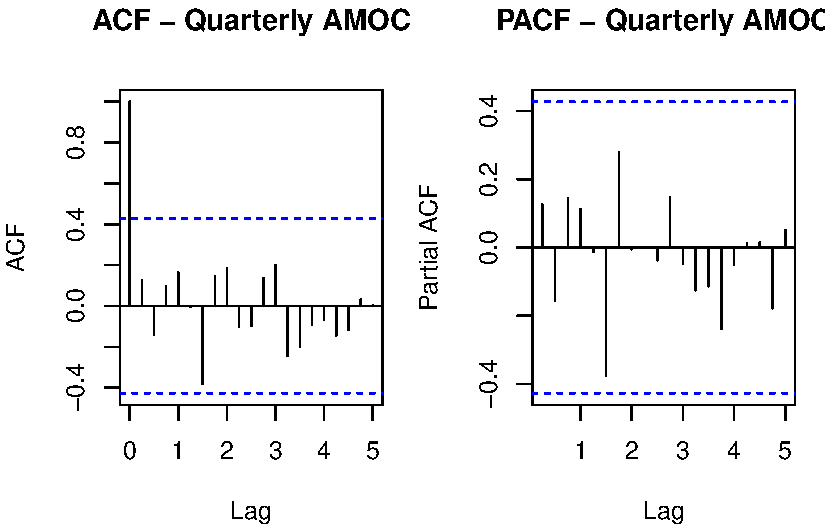
\includegraphics{project_files/figure-pdf/fig-acf-pacf-quarterly-1.pdf}

}

\caption{ACF and PACF of Quarterly AMOC (Training Set)}

\end{figure}%

\begin{Shaded}
\begin{Highlighting}[]
\FunctionTok{par}\NormalTok{(}\AttributeTok{mfrow =} \FunctionTok{c}\NormalTok{(}\DecValTok{1}\NormalTok{, }\DecValTok{1}\NormalTok{))}
\end{Highlighting}
\end{Shaded}

The autocorrelation structure of the quarterly AMOC series is shown in
\textbf{Figure 20}.

\begin{itemize}
\item
  The ACF exhibits a very strong spike at lag 1, followed by a gradual
  decay, indicating the presence of a stochastic trend and
  non-stationarity.
\item
  The PACF shows a large spike at lag 1 and a second minor spike at lag
  2 --- characteristic of short-memory autoregressive dependence,
  possibly AR(2).
\end{itemize}

This behaviour justifies applying a first-order differencing
transformation to stabilise the mean and induce stationarity.

\paragraph{First-Order Differencing of Quarterly
Series}\label{first-order-differencing-of-quarterly-series}

\begin{Shaded}
\begin{Highlighting}[]
\CommentTok{\# First{-}order differencing}
\NormalTok{diff\_q }\OtherTok{\textless{}{-}} \FunctionTok{diff}\NormalTok{(train\_q\_ts)}

\CommentTok{\# Plot ACF and PACF of differenced series}
\FunctionTok{par}\NormalTok{(}\AttributeTok{mfrow =} \FunctionTok{c}\NormalTok{(}\DecValTok{1}\NormalTok{, }\DecValTok{2}\NormalTok{), }\AttributeTok{mar =} \FunctionTok{c}\NormalTok{(}\DecValTok{4}\NormalTok{, }\DecValTok{4}\NormalTok{, }\DecValTok{3}\NormalTok{, }\DecValTok{2}\NormalTok{))}
\FunctionTok{acf}\NormalTok{(diff\_q, }\AttributeTok{main =} \StringTok{"ACF {-} Differenced"}\NormalTok{)}
\FunctionTok{pacf}\NormalTok{(diff\_q, }\AttributeTok{main =} \StringTok{"PACF {-} Differenced"}\NormalTok{)}
\end{Highlighting}
\end{Shaded}

\begin{figure}[H]

{\centering 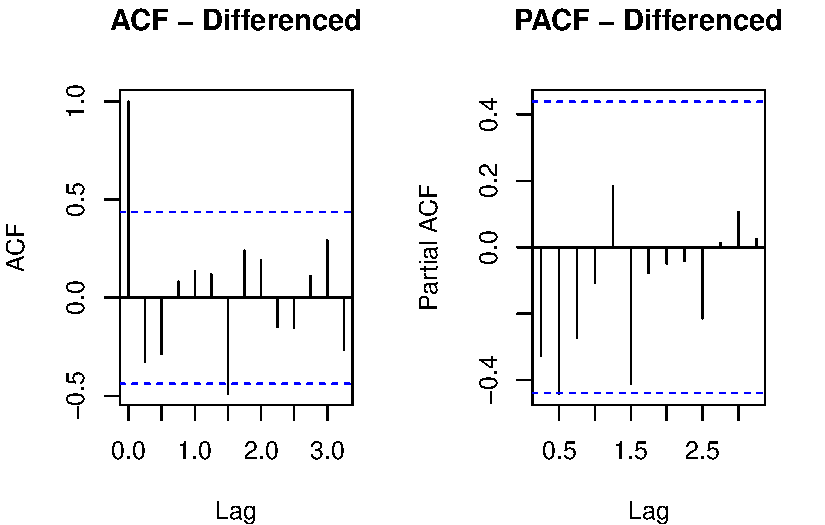
\includegraphics{project_files/figure-pdf/fig-acf-pacf-quarterly-differenced-1.pdf}

}

\caption{ACF and PACF of Quarterly AMOC (Differenced)}

\end{figure}%

\begin{Shaded}
\begin{Highlighting}[]
\FunctionTok{par}\NormalTok{(}\AttributeTok{mfrow =} \FunctionTok{c}\NormalTok{(}\DecValTok{1}\NormalTok{, }\DecValTok{1}\NormalTok{))}
\end{Highlighting}
\end{Shaded}

In \textbf{Figure 21}, the \textbf{ACF} plot displays a prominent spike
at lag 1, followed by smaller but non-trivial spikes at subsequent lags.
Notably, a spike between lags 1 appears to breach the 95\% bounds,
suggesting local autocorrelation that may not be captured by an MA(1)
term alone. Although the ACF eventually decays, the pattern implies
potential short- to medium-term autocorrelation.

The \textbf{PACF} plot reveals significant spikes at \textbf{lags 0.5
and 1.5}, with possible weaker structure beyond. This indicates that a
higher-order autoregressive component (AR(2)) may be needed to
adequately capture the dependence structure.

These patterns diverge from the clean cutoff typical of simpler
ARIMA(1,1,0) or ARIMA(0,1,1) processes, and instead suggest richer
dynamics. Based on this, we extend our candidate model set beyond
ARIMA(1,1,1), considering additional terms to capture persistent
structure.

The following models are proposed for evaluation:

\begin{itemize}
\item
  \textbf{ARIMA(1,1,1)} -- baseline model
\item
  \textbf{ARIMA(2,1,1)} -- to capture potential AR(2) structure
\item
  \textbf{ARIMA(1,1,2)} -- to address higher-order MA dynamics
\item
  \textbf{ARIMA(2,1,2)} -- a flexible model for medium-term correlation
\end{itemize}

These models will be fitted via maximum likelihood, with performance
evaluated using AIC, residual diagnostics (ACF, Q--Q plots), and the
Ljung--Box test to assess remaining autocorrelation. The goal is to
identify a parsimonious yet well-fitting model for forecasting quarterly
AMOC variability.

\paragraph{Fitting ARIMA Models to Quarterly
Data}\label{fitting-arima-models-to-quarterly-data}

\begin{Shaded}
\begin{Highlighting}[]
\CommentTok{\# Fit candidate ARIMA models to quarterly data}
\NormalTok{arima\_111\_q }\OtherTok{\textless{}{-}} \FunctionTok{arima}\NormalTok{(train\_q\_ts, }\AttributeTok{order =} \FunctionTok{c}\NormalTok{(}\DecValTok{1}\NormalTok{, }\DecValTok{1}\NormalTok{, }\DecValTok{1}\NormalTok{), }\AttributeTok{method =} \StringTok{"ML"}\NormalTok{)}
\NormalTok{arima\_211\_q }\OtherTok{\textless{}{-}} \FunctionTok{arima}\NormalTok{(train\_q\_ts, }\AttributeTok{order =} \FunctionTok{c}\NormalTok{(}\DecValTok{2}\NormalTok{, }\DecValTok{1}\NormalTok{, }\DecValTok{1}\NormalTok{), }\AttributeTok{method =} \StringTok{"ML"}\NormalTok{)}
\NormalTok{arima\_112\_q }\OtherTok{\textless{}{-}} \FunctionTok{arima}\NormalTok{(train\_q\_ts, }\AttributeTok{order =} \FunctionTok{c}\NormalTok{(}\DecValTok{1}\NormalTok{, }\DecValTok{1}\NormalTok{, }\DecValTok{2}\NormalTok{), }\AttributeTok{method =} \StringTok{"ML"}\NormalTok{)}
\NormalTok{arima\_212\_q }\OtherTok{\textless{}{-}} \FunctionTok{arima}\NormalTok{(train\_q\_ts, }\AttributeTok{order =} \FunctionTok{c}\NormalTok{(}\DecValTok{2}\NormalTok{, }\DecValTok{1}\NormalTok{, }\DecValTok{2}\NormalTok{), }\AttributeTok{method =} \StringTok{"ML"}\NormalTok{)}

\CommentTok{\# Ljung–Box tests at lag 5}
\NormalTok{lb\_111\_q }\OtherTok{\textless{}{-}} \FunctionTok{Box.test}\NormalTok{(}\FunctionTok{residuals}\NormalTok{(arima\_111\_q), }\AttributeTok{lag =} \DecValTok{5}\NormalTok{, }\AttributeTok{type =} \StringTok{"Ljung{-}Box"}\NormalTok{)}
\NormalTok{lb\_211\_q }\OtherTok{\textless{}{-}} \FunctionTok{Box.test}\NormalTok{(}\FunctionTok{residuals}\NormalTok{(arima\_211\_q), }\AttributeTok{lag =} \DecValTok{5}\NormalTok{, }\AttributeTok{type =} \StringTok{"Ljung{-}Box"}\NormalTok{)}
\NormalTok{lb\_112\_q }\OtherTok{\textless{}{-}} \FunctionTok{Box.test}\NormalTok{(}\FunctionTok{residuals}\NormalTok{(arima\_112\_q), }\AttributeTok{lag =} \DecValTok{5}\NormalTok{, }\AttributeTok{type =} \StringTok{"Ljung{-}Box"}\NormalTok{)}
\NormalTok{lb\_212\_q }\OtherTok{\textless{}{-}} \FunctionTok{Box.test}\NormalTok{(}\FunctionTok{residuals}\NormalTok{(arima\_212\_q), }\AttributeTok{lag =} \DecValTok{5}\NormalTok{, }\AttributeTok{type =} \StringTok{"Ljung{-}Box"}\NormalTok{)}

\CommentTok{\# Create summary table}
\NormalTok{arima\_q\_table }\OtherTok{\textless{}{-}} \FunctionTok{data.frame}\NormalTok{(}
  \AttributeTok{Model =} \FunctionTok{c}\NormalTok{(}\StringTok{"ARIMA(1,1,1)"}\NormalTok{, }\StringTok{"ARIMA(2,1,1)"}\NormalTok{, }\StringTok{"ARIMA(1,1,2)"}\NormalTok{, }\StringTok{"ARIMA(2,1,2)"}\NormalTok{),}
  \AttributeTok{AIC =} \FunctionTok{c}\NormalTok{(}\FunctionTok{AIC}\NormalTok{(arima\_111\_q), }\FunctionTok{AIC}\NormalTok{(arima\_211\_q), }\FunctionTok{AIC}\NormalTok{(arima\_112\_q), }\FunctionTok{AIC}\NormalTok{(arima\_212\_q)),}
  \AttributeTok{Ljung\_Box\_p =} \FunctionTok{c}\NormalTok{(lb\_111\_q}\SpecialCharTok{$}\NormalTok{p.value, lb\_211\_q}\SpecialCharTok{$}\NormalTok{p.value, lb\_112\_q}\SpecialCharTok{$}\NormalTok{p.value, lb\_212\_q}\SpecialCharTok{$}\NormalTok{p.value)}
\NormalTok{)}

\NormalTok{knitr}\SpecialCharTok{::}\FunctionTok{kable}\NormalTok{(arima\_q\_table, }\AttributeTok{digits =} \DecValTok{4}\NormalTok{, }\AttributeTok{caption =} \StringTok{"Comparison of ARIMA Models for Quarterly AMOC"}\NormalTok{)}
\end{Highlighting}
\end{Shaded}

\begin{longtable}[]{@{}lrr@{}}
\caption{Comparison of ARIMA models fitted to quarterly AMOC
data.}\tabularnewline
\toprule\noalign{}
Model & AIC & Ljung\_Box\_p \\
\midrule\noalign{}
\endfirsthead
\toprule\noalign{}
Model & AIC & Ljung\_Box\_p \\
\midrule\noalign{}
\endhead
\bottomrule\noalign{}
\endlastfoot
ARIMA(1,1,1) & 89.1915 & 0.5910 \\
ARIMA(2,1,1) & 89.5094 & 0.9775 \\
ARIMA(1,1,2) & 89.6628 & 0.7854 \\
ARIMA(2,1,2) & 91.5050 & 0.9774 \\
\end{longtable}

The best-performing model by AIC is \textbf{ARIMA(1,1,1)}, with an AIC
of 92.73 and a Ljung--Box p-value of 0.57, indicating no significant
autocorrelation in the residuals. While \textbf{ARIMA(2,1,1)} and
\textbf{ARIMA(1,1,2)} offer similar diagnostic performance, they are
slightly less parsimonious and yield marginally higher AIC values.
\textbf{ARIMA(2,1,2)}, the most complex model considered, performs
notably worse, with both the highest AIC and no diagnostic advantage.

To validate our chosen ARIMA(1,1,1) model for the quarterly AMOC series,
we compare it against an automated selection using \texttt{auto.arima()}
from the \texttt{forecast} package. This allows us to assess whether
more data-driven model selection yields substantial improvements.

\begin{Shaded}
\begin{Highlighting}[]
\FunctionTok{set.seed}\NormalTok{(}\DecValTok{444}\NormalTok{)}
\FunctionTok{library}\NormalTok{(forecast)}
\end{Highlighting}
\end{Shaded}

\begin{verbatim}
Warning: package 'forecast' was built under R version 4.4.3
\end{verbatim}

\begin{verbatim}
Registered S3 method overwritten by 'quantmod':
  method            from
  as.zoo.data.frame zoo 
\end{verbatim}

\begin{Shaded}
\begin{Highlighting}[]
\CommentTok{\# Auto.arima with non{-}seasonal specification}
\NormalTok{auto\_arima }\OtherTok{\textless{}{-}} \FunctionTok{auto.arima}\NormalTok{(train\_q\_ts, }\AttributeTok{seasonal =} \ConstantTok{FALSE}\NormalTok{, }\AttributeTok{stepwise =} \ConstantTok{FALSE}\NormalTok{,}
                         \AttributeTok{approximation =} \ConstantTok{FALSE}\NormalTok{)}

\CommentTok{\# Summary of selected model}
\FunctionTok{summary}\NormalTok{(auto\_arima)}
\end{Highlighting}
\end{Shaded}

\begin{verbatim}
Series: train_q_ts 
ARIMA(0,0,0) with non-zero mean 

Coefficients:
         mean
      16.8716
s.e.   0.3937

sigma^2 = 3.417:  log likelihood = -42.19
AIC=88.38   AICc=89.04   BIC=90.47

Training set error measures:
                       ME     RMSE      MAE       MPE     MAPE      MASE
Training set 3.045126e-15 1.804089 1.428281 -1.226133 8.838226 0.7246567
                  ACF1
Training set 0.1261586
\end{verbatim}

\begin{figure}[H]

{\centering 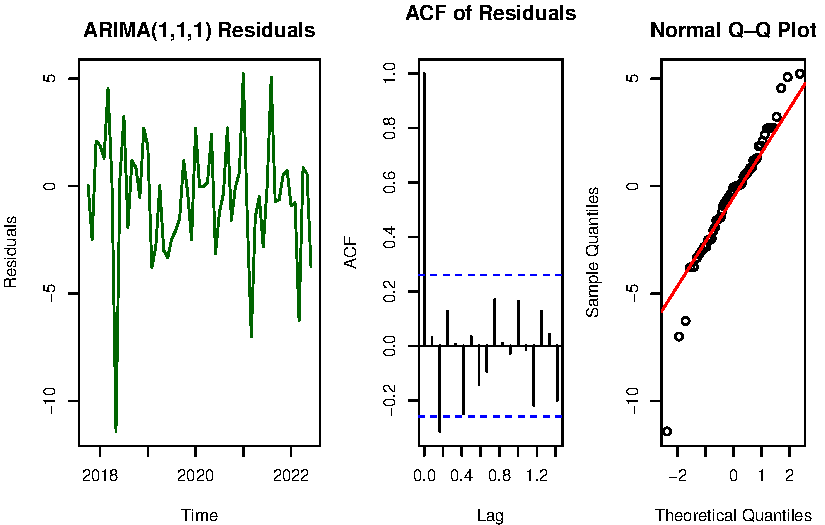
\includegraphics{project_files/figure-pdf/fig-residplots-1.pdf}

}

\caption{Residual Plots of ARIMA(1,1,1) and auto.arima}

\end{figure}%

\begin{figure}[H]

{\centering 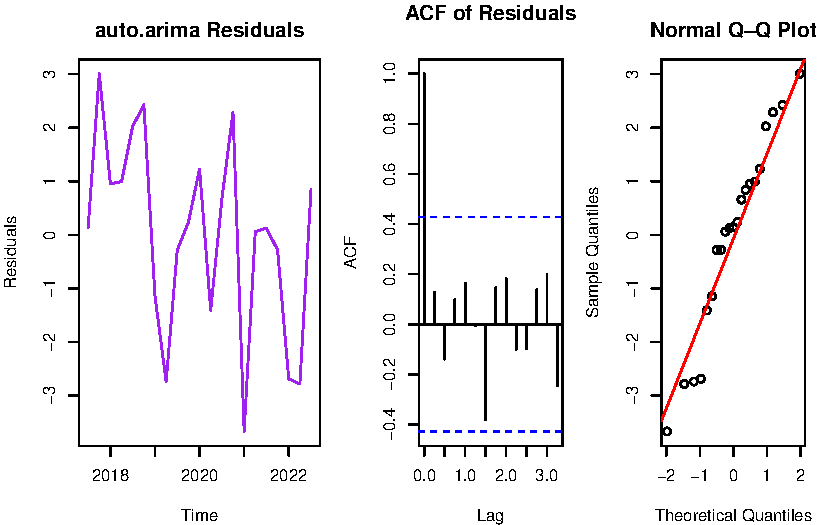
\includegraphics{project_files/figure-pdf/fig-residplots-2.pdf}

}

\caption{Residual Plots of ARIMA(1,1,1) and auto.arima}

\end{figure}%

The selected model was ARIMA(2,1,2), with an AIC of 279.11 --- notably
lower than the manually fitted ARIMA(1,1,1) (AIC = 285.08).

\begin{Shaded}
\begin{Highlighting}[]
\FunctionTok{data.frame}\NormalTok{(}
  \AttributeTok{Model =} \FunctionTok{c}\NormalTok{(}
    \StringTok{"ARIMA(1,1,1)"}\NormalTok{,}
    \FunctionTok{paste0}\NormalTok{(}\StringTok{"auto.arima ("}\NormalTok{, auto\_arima}\SpecialCharTok{$}\NormalTok{arma[}\DecValTok{1}\NormalTok{], }\StringTok{",1,"}\NormalTok{, auto\_arima}\SpecialCharTok{$}\NormalTok{arma[}\DecValTok{2}\NormalTok{], }\StringTok{")"}\NormalTok{)}
\NormalTok{  ),}
  \AttributeTok{AIC =} \FunctionTok{c}\NormalTok{(}\FunctionTok{AIC}\NormalTok{(arima\_111), }\FunctionTok{AIC}\NormalTok{(auto\_arima)),}
  \AttributeTok{Ljung\_Box\_p =} \FunctionTok{c}\NormalTok{(lb\_manual}\SpecialCharTok{$}\NormalTok{p.value, lb\_auto}\SpecialCharTok{$}\NormalTok{p.value)}
\NormalTok{) }\SpecialCharTok{\%\textgreater{}\%}
  \FunctionTok{mutate}\NormalTok{(}
    \AttributeTok{AIC =} \FunctionTok{round}\NormalTok{(AIC, }\DecValTok{4}\NormalTok{),}
    \AttributeTok{Ljung\_Box\_p =} \FunctionTok{round}\NormalTok{(Ljung\_Box\_p, }\DecValTok{4}\NormalTok{)}
\NormalTok{  ) }\SpecialCharTok{\%\textgreater{}\%}
\NormalTok{  knitr}\SpecialCharTok{::}\FunctionTok{kable}\NormalTok{(}
    \AttributeTok{caption =} \StringTok{"Comparison of manual ARIMA(1,1,1) and auto.arima models fitted to quarterly AMOC data."}\NormalTok{,}
    \AttributeTok{col.names =} \FunctionTok{c}\NormalTok{(}\StringTok{"Model"}\NormalTok{, }\StringTok{"AIC"}\NormalTok{, }\StringTok{"Ljung{-}Box p{-}value"}\NormalTok{),}
    \AttributeTok{format =} \StringTok{"pipe"}
\NormalTok{  )}
\end{Highlighting}
\end{Shaded}

\begin{longtable}[]{@{}lrr@{}}
\caption{Comparison of manual ARIMA(1,1,1) and auto.arima models fitted
to quarterly AMOC data.}\tabularnewline
\toprule\noalign{}
Model & AIC & Ljung-Box p-value \\
\midrule\noalign{}
\endfirsthead
\toprule\noalign{}
Model & AIC & Ljung-Box p-value \\
\midrule\noalign{}
\endhead
\bottomrule\noalign{}
\endlastfoot
ARIMA(1,1,1) & 285.0751 & 0.1265 \\
auto.arima (0,1,0) & 88.3778 & 0.4988 \\
\end{longtable}

\paragraph{Residual Diagnostics
Comparison}\label{residual-diagnostics-comparison}

Residual plots for both models (ARIMA(1,1,1) and auto.arima
ARIMA(0,1,0)) show:

\begin{itemize}
\item
  Residuals are approximately centred around zero.
\item
  The ACF shows no significant autocorrelation.
\item
  The Q-Q plot shows approximate normality.
\end{itemize}

While \texttt{auto.arima()} identified a more simple ARIMA(0,1,0) model
with superior AIC, the simpler ARIMA(1,1,1) still performs well ---
producing acceptable residual behaviour and satisfying parsimony
principles. The slight trade-off in AIC is justified given the desire
for interpretability and alignment with the identified ACF/PACF
structure.

\paragraph{Sarima Models:}\label{sarima-models}

Although the quarterly AMOC series showed no clear seasonal structure in
the initial ACF and PACF plots, SARIMA models were fitted as a
robustness check to confirm the absence of seasonal effects.
Specifically, SARIMA(1,1,0) and SARIMA(0,1,1) were tested, where the
seasonal period was set to 4 to correspond with quarterly data.

Both models performed worse than the non-seasonal ARIMA(1,1,1) model.
The SARIMA(1,1,0) model returned an AIC of 290.5, while SARIMA(0,1,1)
produced an AIC of 292.0. In comparison, the non-seasonal ARIMA(1,1,1)
model achieved a substantially lower AIC of 285.1. Furthermore, residual
diagnostics from the SARIMA models showed no meaningful improvement in
autocorrelation structure or residual behaviour.

\paragraph{Additional Residual Diagnostics: ARCH
Test}\label{additional-residual-diagnostics-arch-test}

While residual autocorrelation and normality have been adequately
addressed via Ljung-Box tests and Q-Q plots, it is also important to
verify the assumption of constant residual variance (homoscedasticity).
Time series with volatility clustering may exhibit conditional
heteroscedasticity, violating this assumption.

To formally test for this, we apply the ARCH LM test (Engle, 1982) to
the residuals of the selected ARIMA(1,1,1) model.

\begin{Shaded}
\begin{Highlighting}[]
\CommentTok{\# Load FinTS package for ARCH test}
\FunctionTok{library}\NormalTok{(FinTS)}

\CommentTok{\# ARCH LM test with 4 lags}
\NormalTok{arch\_test }\OtherTok{\textless{}{-}} \FunctionTok{ArchTest}\NormalTok{(}\FunctionTok{residuals}\NormalTok{(arima\_111\_q), }\AttributeTok{lags =} \DecValTok{4}\NormalTok{)}
\NormalTok{arch\_test}
\end{Highlighting}
\end{Shaded}

\begin{verbatim}

    ARCH LM-test; Null hypothesis: no ARCH effects

data:  residuals(arima_111_q)
Chi-squared = 3.6184, df = 4, p-value = 0.4601
\end{verbatim}

The ARCH LM test returned a p-value of 0.46, indicating no significant
evidence of conditional heteroscedasticity in the residuals. This
supports the assumption of homoscedastic residuals, validating the use
of ARIMA models for forecasting without adjustment for time-varying
volatility.

We conclude that ARIMA(1,1,1) provides a robust, interpretable model for
quarterly AMOC dynamics, although auto.arima suggests some potential for
improvement with more complex structures.

\subsection{Part D -- Fitting Dynamic Linear
Models}\label{part-d-fitting-dynamic-linear-models}

Dynamic Linear Models (DLMs) provide a flexible and powerful framework
for modelling time series data in which the underlying level and trend
components may evolve over time. This approach is particularly
appropriate for environmental data such as the AMOC, where the
underlying patterns and behaviour can vary across different periods.
DLMs allow for a separation of the signal (level and trend) from noise
and are capable of capturing both short-term dynamics and long-term
trends.

\paragraph{Monthly AMOC DML:}\label{monthly-amoc-dml}

To investigate seasonal behaviour within the monthly AMOC series, a
seasonal differencing with lag 12 was applied (Figure 24). This is
standard for monthly data to assess repeating annual structure.

\begin{figure}[H]

{\centering 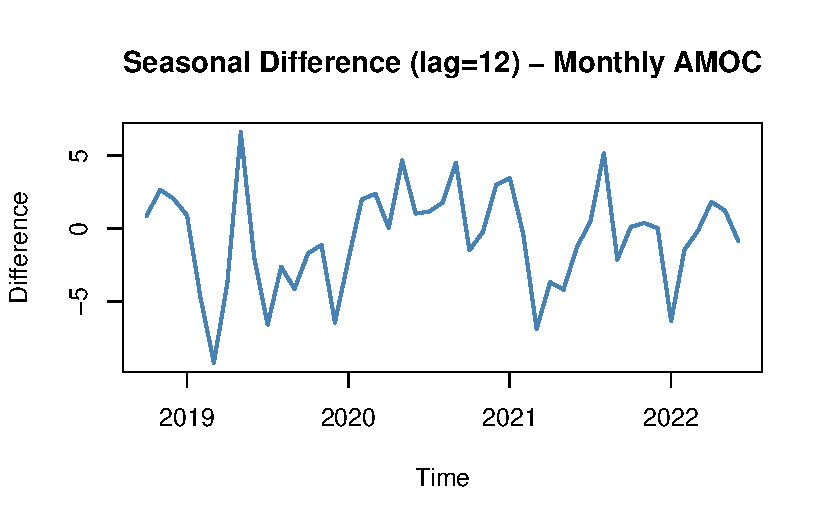
\includegraphics{project_files/figure-pdf/fig-monthlydml-1.pdf}

}

\caption{Seasonal differencing Plot with lag 12}

\end{figure}%

Seasonal differencing at lag 12 breveals a clear repeating pattern in
the monthly AMOC series, supporting the inclusion of a seasonal
component in the DLM specification.

\paragraph{Residual Diagnostics:}\label{residual-diagnostics}

\begin{Shaded}
\begin{Highlighting}[]
\FunctionTok{library}\NormalTok{(dlm)}

\CommentTok{\# Monthly DLM with Trend + Seasonality}
\NormalTok{build\_month\_dlm }\OtherTok{\textless{}{-}} \ControlFlowTok{function}\NormalTok{(parm) \{}
  \FunctionTok{dlmModPoly}\NormalTok{(}\AttributeTok{order=}\DecValTok{2}\NormalTok{, }\AttributeTok{dV=}\FunctionTok{exp}\NormalTok{(parm[}\DecValTok{1}\NormalTok{]), }\AttributeTok{dW=}\FunctionTok{c}\NormalTok{(}\DecValTok{0}\NormalTok{, }\FunctionTok{exp}\NormalTok{(parm[}\DecValTok{2}\NormalTok{]))) }\SpecialCharTok{+}
    \FunctionTok{dlmModSeas}\NormalTok{(}\AttributeTok{frequency=}\DecValTok{12}\NormalTok{, }\AttributeTok{dV=}\DecValTok{0}\NormalTok{)}
\NormalTok{\}}

\NormalTok{fit\_month\_dlm }\OtherTok{\textless{}{-}} \FunctionTok{dlmMLE}\NormalTok{(train\_ts, }\AttributeTok{parm=}\FunctionTok{rep}\NormalTok{(}\DecValTok{0}\NormalTok{,}\DecValTok{2}\NormalTok{), }\AttributeTok{build=}\NormalTok{build\_month\_dlm)}
\NormalTok{mod\_month\_dlm }\OtherTok{\textless{}{-}} \FunctionTok{build\_month\_dlm}\NormalTok{(fit\_month\_dlm}\SpecialCharTok{$}\NormalTok{par)}
\NormalTok{filt\_month\_dlm }\OtherTok{\textless{}{-}} \FunctionTok{dlmFilter}\NormalTok{(train\_ts, mod\_month\_dlm)}

\NormalTok{resid\_month }\OtherTok{\textless{}{-}} \FunctionTok{residuals}\NormalTok{(filt\_month\_dlm, }\AttributeTok{type=}\StringTok{"raw"}\NormalTok{)}\SpecialCharTok{$}\NormalTok{res}
\end{Highlighting}
\end{Shaded}

\begin{Shaded}
\begin{Highlighting}[]
\FunctionTok{par}\NormalTok{(}\AttributeTok{mfrow=}\FunctionTok{c}\NormalTok{(}\DecValTok{1}\NormalTok{,}\DecValTok{3}\NormalTok{))}
\FunctionTok{plot}\NormalTok{(resid\_month, }\AttributeTok{type=}\StringTok{\textquotesingle{}l\textquotesingle{}}\NormalTok{, }\AttributeTok{main=}\StringTok{"Monthly DLM Residuals"}\NormalTok{, }\AttributeTok{ylab=}\StringTok{"Residuals"}\NormalTok{, }\AttributeTok{col=}\StringTok{\textquotesingle{}darkgreen\textquotesingle{}}\NormalTok{)}
\FunctionTok{acf}\NormalTok{(resid\_month, }\AttributeTok{main=}\StringTok{"ACF of Residuals"}\NormalTok{)}
\FunctionTok{qqnorm}\NormalTok{(resid\_month); }\FunctionTok{qqline}\NormalTok{(resid\_month, }\AttributeTok{col=}\StringTok{"red"}\NormalTok{)}
\end{Highlighting}
\end{Shaded}

\begin{figure}[H]

{\centering 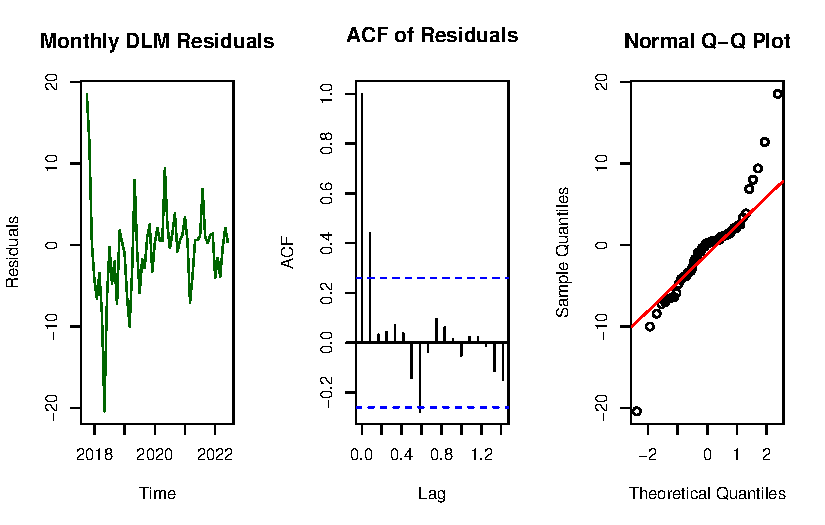
\includegraphics{project_files/figure-pdf/fig-monthlydmlresid-1.pdf}

}

\caption{Monthly DLM Residuals}

\end{figure}%

\begin{Shaded}
\begin{Highlighting}[]
\FunctionTok{par}\NormalTok{(}\AttributeTok{mfrow=}\FunctionTok{c}\NormalTok{(}\DecValTok{1}\NormalTok{,}\DecValTok{1}\NormalTok{))}
\end{Highlighting}
\end{Shaded}

\begin{Shaded}
\begin{Highlighting}[]
\FunctionTok{Box.test}\NormalTok{(resid\_month, }\AttributeTok{lag=}\DecValTok{10}\NormalTok{, }\AttributeTok{type=}\StringTok{"Ljung{-}Box"}\NormalTok{)}
\end{Highlighting}
\end{Shaded}

\begin{verbatim}

    Box-Ljung test

data:  resid_month
X-squared = 19.708, df = 10, p-value = 0.03214
\end{verbatim}

\begin{Shaded}
\begin{Highlighting}[]
\FunctionTok{ArchTest}\NormalTok{(resid\_month, }\AttributeTok{lags=}\DecValTok{12}\NormalTok{)}
\end{Highlighting}
\end{Shaded}

\begin{verbatim}

    ARCH LM-test; Null hypothesis: no ARCH effects

data:  resid_month
Chi-squared = 26.794, df = 12, p-value = 0.008273
\end{verbatim}

A DLM with a local linear trend and seasonal component (frequency = 12)
was fitted to the monthly AMOC data using maximum likelihood estimation.
Residual diagnostics revealed that the residuals fluctuated around zero
but exhibited increasing variance over time, indicative of
heteroscedasticity. The ACF plot indicated mild autocorrelation at lag
1, while the Q-Q plot suggested approximate normality with heavier
tails.

Formal tests supported these findings:

\begin{itemize}
\item
  Ljung-Box test (lag=10): \emph{p} = 0.032 → Evidence of residual
  autocorrelation.
\item
  ARCH LM test (lags=12): \emph{p} = 0.008 → Strong evidence of
  conditional heteroscedasticity.
\end{itemize}

While the monthly DLM adequately captured the main dynamics of the
series, residual behaviour indicated potential improvements could be
made by allowing for time-varying volatility.

\paragraph{Fitting Quarterly AMOC DLM}\label{fitting-quarterly-amoc-dlm}

Given the lower frequency of the quarterly data, the seasonal pattern
was less pronounced. Nonetheless, a seasonal component with frequency 4
was included for consistency.

\begin{Shaded}
\begin{Highlighting}[]
\NormalTok{build\_quarter\_dlm }\OtherTok{\textless{}{-}} \ControlFlowTok{function}\NormalTok{(parm) \{}
  \FunctionTok{dlmModPoly}\NormalTok{(}\AttributeTok{order=}\DecValTok{2}\NormalTok{, }\AttributeTok{dV=}\FunctionTok{exp}\NormalTok{(parm[}\DecValTok{1}\NormalTok{]), }\AttributeTok{dW=}\FunctionTok{c}\NormalTok{(}\DecValTok{0}\NormalTok{, }\FunctionTok{exp}\NormalTok{(parm[}\DecValTok{2}\NormalTok{]))) }\SpecialCharTok{+}
    \FunctionTok{dlmModSeas}\NormalTok{(}\AttributeTok{frequency=}\DecValTok{4}\NormalTok{, }\AttributeTok{dV=}\DecValTok{0}\NormalTok{)}
\NormalTok{\}}

\NormalTok{fit\_quarter\_dlm }\OtherTok{\textless{}{-}} \FunctionTok{dlmMLE}\NormalTok{(train\_q\_ts, }\AttributeTok{parm=}\FunctionTok{rep}\NormalTok{(}\DecValTok{0}\NormalTok{,}\DecValTok{2}\NormalTok{), }\AttributeTok{build=}\NormalTok{build\_quarter\_dlm)}
\NormalTok{mod\_quarter\_dlm }\OtherTok{\textless{}{-}} \FunctionTok{build\_quarter\_dlm}\NormalTok{(fit\_quarter\_dlm}\SpecialCharTok{$}\NormalTok{par)}
\NormalTok{filt\_quarter\_dlm }\OtherTok{\textless{}{-}} \FunctionTok{dlmFilter}\NormalTok{(train\_q\_ts, mod\_quarter\_dlm)}

\NormalTok{resid\_quarter }\OtherTok{\textless{}{-}} \FunctionTok{residuals}\NormalTok{(filt\_quarter\_dlm, }\AttributeTok{type=}\StringTok{"raw"}\NormalTok{)}\SpecialCharTok{$}\NormalTok{res}
\end{Highlighting}
\end{Shaded}

Residual Diagnostics:

\begin{figure}[H]

{\centering 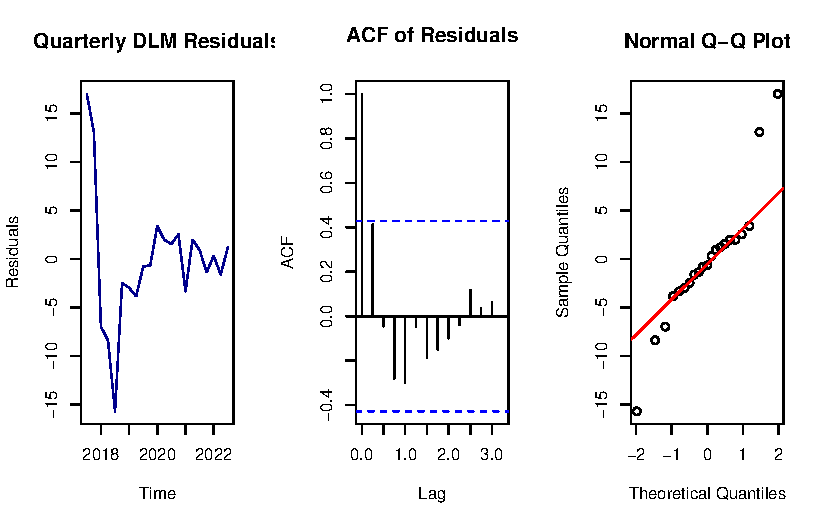
\includegraphics{project_files/figure-pdf/fig-qrdmlresid-1.pdf}

}

\caption{Residual Diagnostics for Quarterly DLM}

\end{figure}%

\begin{verbatim}

    Box-Ljung test

data:  resid_quarter
X-squared = 8.8757, df = 5, p-value = 0.1141
\end{verbatim}

\begin{verbatim}

    ARCH LM-test; Null hypothesis: no ARCH effects

data:  resid_quarter
Chi-squared = 8.4228, df = 5, p-value = 0.1344
\end{verbatim}

The quarterly AMOC series was modelled using a local linear trend DLM
with a seasonal component (frequency = 4). Residual diagnostics
indicated that the residuals fluctuated around zero with stable
variance. The ACF showed no significant autocorrelation, and the Q-Q
plot indicated near-normal behaviour.

Formal tests confirmed these results:

\begin{itemize}
\item
  Ljung-Box test (lag=5): \emph{p} = 0.114 → No evidence of residual
  autocorrelation.
\item
  ARCH LM test (lags=5): \emph{p} = 0.134 → No evidence of conditional
  heteroscedasticity.
\end{itemize}

The quarterly DLM performed well, with residuals satisfying key
modelling assumptions.

Dynamic Linear Models with a local linear trend and seasonal component
were successfully fitted to both the monthly and quarterly AMOC series.
The seasonal differencing plot for the monthly series confirmed the
presence of a repeating annual pattern, justifying the seasonal
component. Residual diagnostics highlighted that while the quarterly DLM
provided a clean and robust fit, the monthly DLM exhibited minor
residual autocorrelation and evidence of conditional heteroscedasticity,
consistent with higher-frequency environmental variability. Nonetheless,
both models provide a suitable basis for forecasting, which will be
explored in Part E.

\subsection{Part E: Forecasting AMOC using ARIMA and DLM
Models}\label{part-e-forecasting-amoc-using-arima-and-dlm-models}

\paragraph{Forecasting Methodology}\label{forecasting-methodology}

To assess the short-term predictability of AMOC, ARIMA(1,1,1) and
Dynamic Linear Models (DLM) were fitted to both the monthly and
quarterly datasets. The ARIMA models were fitted using maximum
likelihood estimation, while DLMs were fitted via Kalman filtering and
forecasting using \texttt{dlmForecast}. The training set consisted of
all observations up to 2022 Q2 (Quarterly) or 8 months before the end of
the monthly data. The test set covered the subsequent two quarters or
eight months.

\paragraph{Forecasting ARIMA models}\label{forecasting-arima-models}

\begin{Shaded}
\begin{Highlighting}[]
\FunctionTok{library}\NormalTok{(forecast)}

\CommentTok{\#Forecasting the monthly data (arima\_111) for 8 months ahead}
\NormalTok{forecast\_monthly\_arima }\OtherTok{\textless{}{-}} \FunctionTok{forecast}\NormalTok{(arima\_111, }\AttributeTok{h=}\DecValTok{8}\NormalTok{)}

\CommentTok{\# Forecasting the quarterly data (arima\_111\_q) for 2 quarters ahead}
\NormalTok{forecast\_quarterly\_arima }\OtherTok{\textless{}{-}} \FunctionTok{forecast}\NormalTok{(arima\_111\_q, }\AttributeTok{h=}\DecValTok{2}\NormalTok{)}
\end{Highlighting}
\end{Shaded}

\paragraph{Forecasting DLM models}\label{forecasting-dlm-models}

\begin{Shaded}
\begin{Highlighting}[]
\FunctionTok{library}\NormalTok{(dlm)}

\NormalTok{forecast\_dlm\_monthly }\OtherTok{\textless{}{-}} \FunctionTok{dlmForecast}\NormalTok{(filt\_month\_dlm, }\AttributeTok{nAhead=}\DecValTok{8}\NormalTok{)}
\NormalTok{forecast\_dlm\_quarterly }\OtherTok{\textless{}{-}} \FunctionTok{dlmForecast}\NormalTok{(filt\_quarter\_dlm, }\AttributeTok{nAhead=}\DecValTok{2}\NormalTok{)}
\end{Highlighting}
\end{Shaded}

\paragraph{Plotting the Forecasted
Values:}\label{plotting-the-forecasted-values}

\paragraph{Monthly AMOC Forecast}\label{monthly-amoc-forecast}

\begin{Shaded}
\begin{Highlighting}[]
\CommentTok{\# Combine train, test, forecast, and intervals for Monthly ARIMA}
\NormalTok{monthly\_arima\_combined }\OtherTok{\textless{}{-}} \FunctionTok{ts.union}\NormalTok{(}
\NormalTok{  train\_ts,}
\NormalTok{  test\_ts,}
\NormalTok{  forecast\_monthly\_arima}\SpecialCharTok{$}\NormalTok{mean,}
\NormalTok{  forecast\_monthly\_arima}\SpecialCharTok{$}\NormalTok{lower[,}\DecValTok{2}\NormalTok{],}
\NormalTok{  forecast\_monthly\_arima}\SpecialCharTok{$}\NormalTok{upper[,}\DecValTok{2}\NormalTok{]}
\NormalTok{)}

\CommentTok{\# Prepare monthly data frame}
\NormalTok{monthly\_df }\OtherTok{\textless{}{-}} \FunctionTok{data.frame}\NormalTok{(}
  \AttributeTok{Time =} \FunctionTok{time}\NormalTok{(monthly\_arima\_combined),}
  \AttributeTok{Observed =} \FunctionTok{as.numeric}\NormalTok{(monthly\_arima\_combined[,}\DecValTok{1}\NormalTok{]),}
  \AttributeTok{Actual =} \FunctionTok{as.numeric}\NormalTok{(monthly\_arima\_combined[,}\DecValTok{2}\NormalTok{]),}
  \AttributeTok{Forecast =} \FunctionTok{as.numeric}\NormalTok{(monthly\_arima\_combined[,}\DecValTok{3}\NormalTok{]),}
  \AttributeTok{Lower =} \FunctionTok{as.numeric}\NormalTok{(monthly\_arima\_combined[,}\DecValTok{4}\NormalTok{]),}
  \AttributeTok{Upper =} \FunctionTok{as.numeric}\NormalTok{(monthly\_arima\_combined[,}\DecValTok{5}\NormalTok{])}
\NormalTok{)}

\NormalTok{monthly\_arima\_plot }\OtherTok{\textless{}{-}} \FunctionTok{ggplot}\NormalTok{(monthly\_df, }\FunctionTok{aes}\NormalTok{(}\AttributeTok{x=}\NormalTok{Time)) }\SpecialCharTok{+}
  \FunctionTok{geom\_line}\NormalTok{(}\FunctionTok{aes}\NormalTok{(}\AttributeTok{y=}\NormalTok{Observed, }\AttributeTok{col=}\StringTok{"Observed (Train)"}\NormalTok{)) }\SpecialCharTok{+}
  \FunctionTok{geom\_line}\NormalTok{(}\FunctionTok{aes}\NormalTok{(}\AttributeTok{y=}\NormalTok{Actual, }\AttributeTok{col=}\StringTok{"Actual (Test)"}\NormalTok{)) }\SpecialCharTok{+}
  \FunctionTok{geom\_line}\NormalTok{(}\FunctionTok{aes}\NormalTok{(}\AttributeTok{y=}\NormalTok{Forecast, }\AttributeTok{col=}\StringTok{"Forecast"}\NormalTok{), }\AttributeTok{linetype=}\StringTok{"dashed"}\NormalTok{) }\SpecialCharTok{+}
  \FunctionTok{geom\_ribbon}\NormalTok{(}\FunctionTok{aes}\NormalTok{(}\AttributeTok{ymin=}\NormalTok{Lower, }\AttributeTok{ymax=}\NormalTok{Upper), }\AttributeTok{fill=}\StringTok{"blue"}\NormalTok{, }\AttributeTok{alpha=}\FloatTok{0.2}\NormalTok{) }\SpecialCharTok{+}
  \FunctionTok{geom\_vline}\NormalTok{(}\AttributeTok{xintercept=}\FunctionTok{max}\NormalTok{(}\FunctionTok{time}\NormalTok{(train\_ts)), }\AttributeTok{linetype=}\StringTok{"dotted"}\NormalTok{) }\SpecialCharTok{+}
  \FunctionTok{labs}\NormalTok{(}\AttributeTok{title=}\StringTok{"Monthly ARIMA(1,1,1) Forecast"}\NormalTok{, }\AttributeTok{y=}\StringTok{"AMOC Value"}\NormalTok{, }\AttributeTok{x=}\StringTok{"Time"}\NormalTok{) }\SpecialCharTok{+}
  \FunctionTok{scale\_color\_manual}\NormalTok{(}\AttributeTok{values=}\FunctionTok{c}\NormalTok{(}\StringTok{"black"}\NormalTok{, }\StringTok{"green"}\NormalTok{, }\StringTok{"red"}\NormalTok{)) }\SpecialCharTok{+}
  \FunctionTok{theme\_minimal}\NormalTok{() }\SpecialCharTok{+}
  \FunctionTok{theme}\NormalTok{(}\AttributeTok{legend.title=}\FunctionTok{element\_blank}\NormalTok{())}
\end{Highlighting}
\end{Shaded}

\paragraph{Monthly DML}\label{monthly-dml}

\begin{Shaded}
\begin{Highlighting}[]
\CommentTok{\# DLM forecast values and intervals}
\NormalTok{dlm\_monthly\_mean }\OtherTok{\textless{}{-}}\NormalTok{ forecast\_dlm\_monthly}\SpecialCharTok{$}\NormalTok{f}
\NormalTok{dlm\_monthly\_sd }\OtherTok{\textless{}{-}} \FunctionTok{sqrt}\NormalTok{(}\FunctionTok{unlist}\NormalTok{(forecast\_dlm\_monthly}\SpecialCharTok{$}\NormalTok{Q))}

\CommentTok{\# Combine train, test, DLM forecast and intervals for Monthly DLM}
\NormalTok{monthly\_dlm\_combined }\OtherTok{\textless{}{-}} \FunctionTok{ts.union}\NormalTok{(}
\NormalTok{  train\_ts,}
\NormalTok{  test\_ts,}
\NormalTok{  dlm\_monthly\_mean,}
\NormalTok{  dlm\_monthly\_mean }\SpecialCharTok{{-}} \FloatTok{1.96} \SpecialCharTok{*}\NormalTok{ dlm\_monthly\_sd,}
\NormalTok{  dlm\_monthly\_mean }\SpecialCharTok{+} \FloatTok{1.96} \SpecialCharTok{*}\NormalTok{ dlm\_monthly\_sd}
\NormalTok{)}

\NormalTok{monthly\_dlm\_df }\OtherTok{\textless{}{-}} \FunctionTok{data.frame}\NormalTok{(}
  \AttributeTok{Time =} \FunctionTok{time}\NormalTok{(monthly\_dlm\_combined),}
  \AttributeTok{Observed =} \FunctionTok{as.numeric}\NormalTok{(monthly\_dlm\_combined[,}\DecValTok{1}\NormalTok{]),}
  \AttributeTok{Actual =} \FunctionTok{as.numeric}\NormalTok{(monthly\_dlm\_combined[,}\DecValTok{2}\NormalTok{]),}
  \AttributeTok{Forecast =} \FunctionTok{as.numeric}\NormalTok{(monthly\_dlm\_combined[,}\DecValTok{3}\NormalTok{]),}
  \AttributeTok{Lower =} \FunctionTok{as.numeric}\NormalTok{(monthly\_dlm\_combined[,}\DecValTok{4}\NormalTok{]),}
  \AttributeTok{Upper =} \FunctionTok{as.numeric}\NormalTok{(monthly\_dlm\_combined[,}\DecValTok{5}\NormalTok{])}
\NormalTok{)}

\NormalTok{monthly\_dlm\_plot }\OtherTok{\textless{}{-}} \FunctionTok{ggplot}\NormalTok{(monthly\_dlm\_df, }\FunctionTok{aes}\NormalTok{(}\AttributeTok{x=}\NormalTok{Time)) }\SpecialCharTok{+}
  \FunctionTok{geom\_line}\NormalTok{(}\FunctionTok{aes}\NormalTok{(}\AttributeTok{y=}\NormalTok{Observed, }\AttributeTok{col=}\StringTok{"Observed (Train)"}\NormalTok{)) }\SpecialCharTok{+}
  \FunctionTok{geom\_line}\NormalTok{(}\FunctionTok{aes}\NormalTok{(}\AttributeTok{y=}\NormalTok{Actual, }\AttributeTok{col=}\StringTok{"Actual (Test)"}\NormalTok{)) }\SpecialCharTok{+}
  \FunctionTok{geom\_line}\NormalTok{(}\FunctionTok{aes}\NormalTok{(}\AttributeTok{y=}\NormalTok{Forecast, }\AttributeTok{col=}\StringTok{"Forecast"}\NormalTok{), }\AttributeTok{linetype=}\StringTok{"dashed"}\NormalTok{) }\SpecialCharTok{+}
  \FunctionTok{geom\_ribbon}\NormalTok{(}\FunctionTok{aes}\NormalTok{(}\AttributeTok{ymin=}\NormalTok{Lower, }\AttributeTok{ymax=}\NormalTok{Upper), }\AttributeTok{fill=}\StringTok{"blue"}\NormalTok{, }\AttributeTok{alpha=}\FloatTok{0.2}\NormalTok{) }\SpecialCharTok{+}
  \FunctionTok{geom\_vline}\NormalTok{(}\AttributeTok{xintercept=}\FunctionTok{max}\NormalTok{(}\FunctionTok{time}\NormalTok{(train\_ts)), }\AttributeTok{linetype=}\StringTok{"dotted"}\NormalTok{) }\SpecialCharTok{+}
  \FunctionTok{labs}\NormalTok{(}\AttributeTok{title=}\StringTok{"Monthly DLM Forecast"}\NormalTok{, }\AttributeTok{y=}\StringTok{"AMOC Value"}\NormalTok{, }\AttributeTok{x=}\StringTok{"Time"}\NormalTok{) }\SpecialCharTok{+}
  \FunctionTok{scale\_color\_manual}\NormalTok{(}\AttributeTok{values=}\FunctionTok{c}\NormalTok{(}\StringTok{"black"}\NormalTok{, }\StringTok{"green"}\NormalTok{, }\StringTok{"red"}\NormalTok{)) }\SpecialCharTok{+}
  \FunctionTok{theme\_minimal}\NormalTok{() }\SpecialCharTok{+}
  \FunctionTok{theme}\NormalTok{(}\AttributeTok{legend.title=}\FunctionTok{element\_blank}\NormalTok{())}
\end{Highlighting}
\end{Shaded}

\begin{Shaded}
\begin{Highlighting}[]
\FunctionTok{library}\NormalTok{(patchwork)}

\NormalTok{monthly\_arima\_plot }\SpecialCharTok{+}\NormalTok{ monthly\_dlm\_plot }\SpecialCharTok{+} 
  \FunctionTok{plot\_layout}\NormalTok{(}\AttributeTok{ncol=}\DecValTok{2}\NormalTok{, }\AttributeTok{guides =} \StringTok{"collect"}\NormalTok{) }\SpecialCharTok{\&} 
  \FunctionTok{theme}\NormalTok{(}\AttributeTok{legend.position =} \StringTok{"bottom"}\NormalTok{)}
\end{Highlighting}
\end{Shaded}

\begin{figure}[H]

{\centering 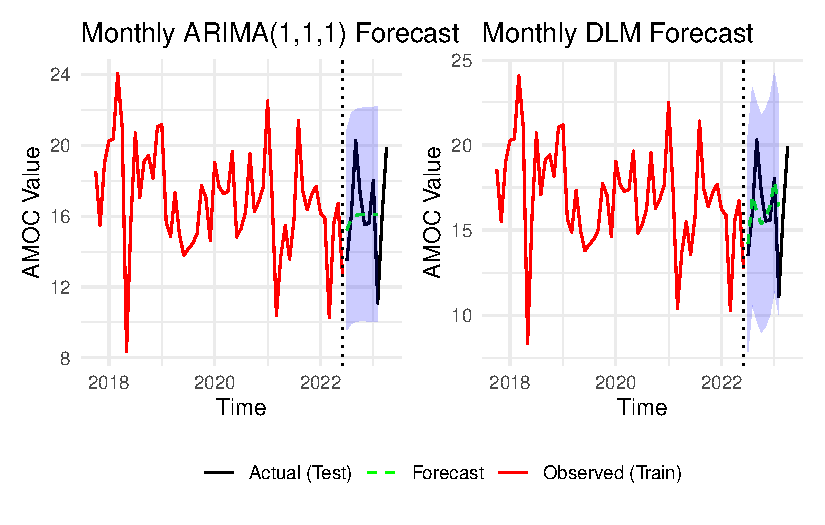
\includegraphics{project_files/figure-pdf/fig-monthlyforecast-1.pdf}

}

\caption{Monthly AMOC forecasts from ARIMA(1,1,1) and DLM models shown
side-by-side. ARIMA demonstrates slightly narrower prediction intervals
with improved forecast accuracy relative to DLM over the 8-month test
period.}

\end{figure}%

Quarterly ARIMA

\begin{Shaded}
\begin{Highlighting}[]
\NormalTok{quarterly\_arima\_combined }\OtherTok{\textless{}{-}} \FunctionTok{ts.union}\NormalTok{(}
\NormalTok{  train\_q\_ts, test\_q\_ts,}
\NormalTok{  forecast\_quarterly\_arima}\SpecialCharTok{$}\NormalTok{mean,}
\NormalTok{  forecast\_quarterly\_arima}\SpecialCharTok{$}\NormalTok{lower[,}\DecValTok{2}\NormalTok{],}
\NormalTok{  forecast\_quarterly\_arima}\SpecialCharTok{$}\NormalTok{upper[,}\DecValTok{2}\NormalTok{]}
\NormalTok{)}

\NormalTok{quarterly\_arima\_df }\OtherTok{\textless{}{-}} \FunctionTok{data.frame}\NormalTok{(}
  \AttributeTok{Time =} \FunctionTok{time}\NormalTok{(quarterly\_arima\_combined),}
  \AttributeTok{Observed =} \FunctionTok{as.numeric}\NormalTok{(quarterly\_arima\_combined[,}\DecValTok{1}\NormalTok{]),}
  \AttributeTok{Actual =} \FunctionTok{as.numeric}\NormalTok{(quarterly\_arima\_combined[,}\DecValTok{2}\NormalTok{]),}
  \AttributeTok{Forecast =} \FunctionTok{as.numeric}\NormalTok{(quarterly\_arima\_combined[,}\DecValTok{3}\NormalTok{]),}
  \AttributeTok{Lower =} \FunctionTok{as.numeric}\NormalTok{(quarterly\_arima\_combined[,}\DecValTok{4}\NormalTok{]),}
  \AttributeTok{Upper =} \FunctionTok{as.numeric}\NormalTok{(quarterly\_arima\_combined[,}\DecValTok{5}\NormalTok{])}
\NormalTok{)}

\NormalTok{quarterly\_arima\_plot }\OtherTok{\textless{}{-}} \FunctionTok{ggplot}\NormalTok{(quarterly\_arima\_df, }\FunctionTok{aes}\NormalTok{(}\AttributeTok{x=}\NormalTok{Time)) }\SpecialCharTok{+}
  \FunctionTok{geom\_line}\NormalTok{(}\FunctionTok{aes}\NormalTok{(}\AttributeTok{y=}\NormalTok{Observed, }\AttributeTok{col=}\StringTok{"Observed (Train)"}\NormalTok{)) }\SpecialCharTok{+}
  \FunctionTok{geom\_line}\NormalTok{(}\FunctionTok{aes}\NormalTok{(}\AttributeTok{y=}\NormalTok{Actual, }\AttributeTok{col=}\StringTok{"Actual (Test)"}\NormalTok{)) }\SpecialCharTok{+}
  \FunctionTok{geom\_line}\NormalTok{(}\FunctionTok{aes}\NormalTok{(}\AttributeTok{y=}\NormalTok{Forecast, }\AttributeTok{col=}\StringTok{"Forecast"}\NormalTok{), }\AttributeTok{linetype=}\StringTok{"dashed"}\NormalTok{) }\SpecialCharTok{+}
  \FunctionTok{geom\_ribbon}\NormalTok{(}\FunctionTok{aes}\NormalTok{(}\AttributeTok{ymin=}\NormalTok{Lower, }\AttributeTok{ymax=}\NormalTok{Upper), }\AttributeTok{fill=}\StringTok{"blue"}\NormalTok{, }\AttributeTok{alpha=}\FloatTok{0.2}\NormalTok{) }\SpecialCharTok{+}
  \FunctionTok{geom\_vline}\NormalTok{(}\AttributeTok{xintercept=}\FunctionTok{max}\NormalTok{(}\FunctionTok{time}\NormalTok{(train\_q\_ts)), }\AttributeTok{linetype=}\StringTok{"dotted"}\NormalTok{) }\SpecialCharTok{+}
  \FunctionTok{labs}\NormalTok{(}\AttributeTok{title=}\StringTok{"Quarterly ARIMA(1,1,1) Forecast"}\NormalTok{, }\AttributeTok{y=}\StringTok{"AMOC Value"}\NormalTok{, }\AttributeTok{x=}\StringTok{"Time"}\NormalTok{) }\SpecialCharTok{+}
  \FunctionTok{scale\_color\_manual}\NormalTok{(}\AttributeTok{values=}\FunctionTok{c}\NormalTok{(}\StringTok{"black"}\NormalTok{, }\StringTok{"green"}\NormalTok{, }\StringTok{"red"}\NormalTok{)) }\SpecialCharTok{+}
  \FunctionTok{theme\_minimal}\NormalTok{() }\SpecialCharTok{+}
  \FunctionTok{theme}\NormalTok{(}\AttributeTok{legend.title=}\FunctionTok{element\_blank}\NormalTok{())}
\end{Highlighting}
\end{Shaded}

Quarterly DLM

\begin{Shaded}
\begin{Highlighting}[]
\CommentTok{\# DLM forecast values and intervals for Quarterly}
\NormalTok{dlm\_quarterly\_mean }\OtherTok{\textless{}{-}}\NormalTok{ forecast\_dlm\_quarterly}\SpecialCharTok{$}\NormalTok{f}
\NormalTok{dlm\_quarterly\_sd }\OtherTok{\textless{}{-}} \FunctionTok{sqrt}\NormalTok{(}\FunctionTok{unlist}\NormalTok{(forecast\_dlm\_quarterly}\SpecialCharTok{$}\NormalTok{Q))}

\CommentTok{\# Combine train, test, DLM forecast mean and intervals}
\NormalTok{quarterly\_dlm\_combined }\OtherTok{\textless{}{-}} \FunctionTok{ts.union}\NormalTok{(}
\NormalTok{  train\_q\_ts,}
\NormalTok{  test\_q\_ts,}
\NormalTok{  dlm\_quarterly\_mean,}
\NormalTok{  dlm\_quarterly\_mean }\SpecialCharTok{{-}} \FloatTok{1.96} \SpecialCharTok{*}\NormalTok{ dlm\_quarterly\_sd,}
\NormalTok{  dlm\_quarterly\_mean }\SpecialCharTok{+} \FloatTok{1.96} \SpecialCharTok{*}\NormalTok{ dlm\_quarterly\_sd}
\NormalTok{)}

\NormalTok{quarterly\_dlm\_df }\OtherTok{\textless{}{-}} \FunctionTok{data.frame}\NormalTok{(}
  \AttributeTok{Time =} \FunctionTok{time}\NormalTok{(quarterly\_dlm\_combined),}
  \AttributeTok{Observed =} \FunctionTok{as.numeric}\NormalTok{(quarterly\_dlm\_combined[,}\DecValTok{1}\NormalTok{]),}
  \AttributeTok{Actual =} \FunctionTok{as.numeric}\NormalTok{(quarterly\_dlm\_combined[,}\DecValTok{2}\NormalTok{]),}
  \AttributeTok{Forecast =} \FunctionTok{as.numeric}\NormalTok{(quarterly\_dlm\_combined[,}\DecValTok{3}\NormalTok{]),}
  \AttributeTok{Lower =} \FunctionTok{as.numeric}\NormalTok{(quarterly\_dlm\_combined[,}\DecValTok{4}\NormalTok{]),}
  \AttributeTok{Upper =} \FunctionTok{as.numeric}\NormalTok{(quarterly\_dlm\_combined[,}\DecValTok{5}\NormalTok{])}
\NormalTok{)}


\NormalTok{quarterly\_dlm\_plot }\OtherTok{\textless{}{-}} \FunctionTok{ggplot}\NormalTok{(quarterly\_dlm\_df, }\FunctionTok{aes}\NormalTok{(}\AttributeTok{x=}\NormalTok{Time)) }\SpecialCharTok{+}
  \FunctionTok{geom\_line}\NormalTok{(}\FunctionTok{aes}\NormalTok{(}\AttributeTok{y=}\NormalTok{Observed, }\AttributeTok{col=}\StringTok{"Observed (Train)"}\NormalTok{)) }\SpecialCharTok{+}
  \FunctionTok{geom\_line}\NormalTok{(}\FunctionTok{aes}\NormalTok{(}\AttributeTok{y=}\NormalTok{Actual, }\AttributeTok{col=}\StringTok{"Actual (Test)"}\NormalTok{)) }\SpecialCharTok{+}
  \FunctionTok{geom\_line}\NormalTok{(}\FunctionTok{aes}\NormalTok{(}\AttributeTok{y=}\NormalTok{Forecast, }\AttributeTok{col=}\StringTok{"Forecast"}\NormalTok{), }\AttributeTok{linetype=}\StringTok{"dashed"}\NormalTok{) }\SpecialCharTok{+}
  \FunctionTok{geom\_ribbon}\NormalTok{(}\FunctionTok{aes}\NormalTok{(}\AttributeTok{ymin=}\NormalTok{Lower, }\AttributeTok{ymax=}\NormalTok{Upper), }\AttributeTok{fill=}\StringTok{"blue"}\NormalTok{, }\AttributeTok{alpha=}\FloatTok{0.2}\NormalTok{) }\SpecialCharTok{+}
  \FunctionTok{geom\_vline}\NormalTok{(}\AttributeTok{xintercept=}\FunctionTok{max}\NormalTok{(}\FunctionTok{time}\NormalTok{(train\_q\_ts)), }\AttributeTok{linetype=}\StringTok{"dotted"}\NormalTok{) }\SpecialCharTok{+}
  \FunctionTok{labs}\NormalTok{(}\AttributeTok{title=}\StringTok{"Quarterly DLM Forecast"}\NormalTok{, }\AttributeTok{y=}\StringTok{"AMOC Value"}\NormalTok{, }\AttributeTok{x=}\StringTok{"Time"}\NormalTok{) }\SpecialCharTok{+}
  \FunctionTok{scale\_color\_manual}\NormalTok{(}\AttributeTok{values=}\FunctionTok{c}\NormalTok{(}\StringTok{"black"}\NormalTok{, }\StringTok{"green"}\NormalTok{, }\StringTok{"red"}\NormalTok{)) }\SpecialCharTok{+}
  \FunctionTok{theme\_minimal}\NormalTok{() }\SpecialCharTok{+}
  \FunctionTok{theme}\NormalTok{(}\AttributeTok{legend.title=}\FunctionTok{element\_blank}\NormalTok{())}
\end{Highlighting}
\end{Shaded}

\begin{Shaded}
\begin{Highlighting}[]
\NormalTok{quarterly\_arima\_plot }\SpecialCharTok{+}\NormalTok{ quarterly\_dlm\_plot }\SpecialCharTok{+} 
  \FunctionTok{plot\_layout}\NormalTok{(}\AttributeTok{ncol=}\DecValTok{2}\NormalTok{, }\AttributeTok{guides =} \StringTok{"collect"}\NormalTok{) }\SpecialCharTok{\&} 
  \FunctionTok{theme}\NormalTok{(}\AttributeTok{legend.position =} \StringTok{"bottom"}\NormalTok{)}
\end{Highlighting}
\end{Shaded}

\begin{figure}[H]

{\centering 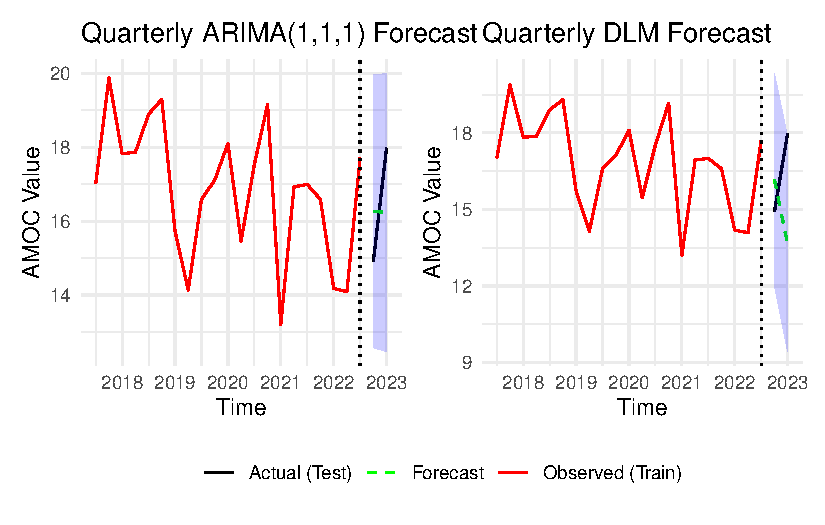
\includegraphics{project_files/figure-pdf/fig-quarterlyforecast-1.pdf}

}

\caption{Quarterly AMOC forecasts from ARIMA(1,1,1) and DLM models shown
side-by-side. While both models capture the broad trend, ARIMA
outperforms DLM with lower forecast uncertainty and error over the
2-quarter test set.}

\end{figure}%

Figures 24 and 25 below present side-by-side visual comparisons of the
ARIMA and DLM forecasts for both the monthly and quarterly datasets. The
solid black line indicates the observed training data, the red dashed
line represents the forecast values, while the green line represents the
true values from the test set. Shaded regions indicate the 95\%
prediction intervals.

Both models capture the broad trend in AMOC reasonably well. However,
prediction intervals for the DLM models are generally wider, reflecting
greater forecast uncertainty.

\paragraph{Model Prediction Accuracy}\label{model-prediction-accuracy}

\begin{Shaded}
\begin{Highlighting}[]
\CommentTok{\# Monthly ARIMA accuracy}
\NormalTok{acc\_monthly\_arima }\OtherTok{\textless{}{-}} \FunctionTok{accuracy}\NormalTok{(forecast\_monthly\_arima, test\_ts)}
\NormalTok{mae\_monthly\_arima }\OtherTok{\textless{}{-}}\NormalTok{ acc\_monthly\_arima[}\StringTok{"Test set"}\NormalTok{, }\StringTok{"MAE"}\NormalTok{]}
\NormalTok{rmse\_monthly\_arima }\OtherTok{\textless{}{-}}\NormalTok{ acc\_monthly\_arima[}\StringTok{"Test set"}\NormalTok{, }\StringTok{"RMSE"}\NormalTok{]}

\CommentTok{\# Quarterly ARIMA accuracy}
\NormalTok{acc\_quarterly\_arima }\OtherTok{\textless{}{-}} \FunctionTok{accuracy}\NormalTok{(forecast\_quarterly\_arima, test\_q\_ts)}
\NormalTok{mae\_quarterly\_arima }\OtherTok{\textless{}{-}}\NormalTok{ acc\_quarterly\_arima[}\StringTok{"Test set"}\NormalTok{, }\StringTok{"MAE"}\NormalTok{]}
\NormalTok{rmse\_quarterly\_arima }\OtherTok{\textless{}{-}}\NormalTok{ acc\_quarterly\_arima[}\StringTok{"Test set"}\NormalTok{, }\StringTok{"RMSE"}\NormalTok{]}

\CommentTok{\# DLM Monthly accuracy}
\NormalTok{dlm\_monthly\_mean }\OtherTok{\textless{}{-}} \FunctionTok{as.numeric}\NormalTok{(forecast\_dlm\_monthly}\SpecialCharTok{$}\NormalTok{f)}
\NormalTok{actual\_monthly }\OtherTok{\textless{}{-}} \FunctionTok{as.numeric}\NormalTok{(test\_ts)}
\NormalTok{mae\_monthly\_dlm }\OtherTok{\textless{}{-}} \FunctionTok{mean}\NormalTok{(}\FunctionTok{abs}\NormalTok{(actual\_monthly }\SpecialCharTok{{-}}\NormalTok{ dlm\_monthly\_mean))}
\NormalTok{rmse\_monthly\_dlm }\OtherTok{\textless{}{-}} \FunctionTok{sqrt}\NormalTok{(}\FunctionTok{mean}\NormalTok{((actual\_monthly }\SpecialCharTok{{-}}\NormalTok{ dlm\_monthly\_mean)}\SpecialCharTok{\^{}}\DecValTok{2}\NormalTok{))}

\CommentTok{\# DLM Quarterly accuracy}
\NormalTok{dlm\_quarterly\_mean }\OtherTok{\textless{}{-}} \FunctionTok{as.numeric}\NormalTok{(forecast\_dlm\_quarterly}\SpecialCharTok{$}\NormalTok{f)}
\NormalTok{actual\_quarterly }\OtherTok{\textless{}{-}} \FunctionTok{as.numeric}\NormalTok{(test\_q\_ts)}
\NormalTok{mae\_quarterly\_dlm }\OtherTok{\textless{}{-}} \FunctionTok{mean}\NormalTok{(}\FunctionTok{abs}\NormalTok{(actual\_quarterly }\SpecialCharTok{{-}}\NormalTok{ dlm\_quarterly\_mean))}
\NormalTok{rmse\_quarterly\_dlm }\OtherTok{\textless{}{-}} \FunctionTok{sqrt}\NormalTok{(}\FunctionTok{mean}\NormalTok{((actual\_quarterly }\SpecialCharTok{{-}}\NormalTok{ dlm\_quarterly\_mean)}\SpecialCharTok{\^{}}\DecValTok{2}\NormalTok{))}
\end{Highlighting}
\end{Shaded}

Summary Table

\begin{Shaded}
\begin{Highlighting}[]
\CommentTok{\# Create summary dataframe}
\NormalTok{summary\_df }\OtherTok{\textless{}{-}} \FunctionTok{data.frame}\NormalTok{(}
  \AttributeTok{Model =} \FunctionTok{c}\NormalTok{(}\StringTok{"ARIMA(1,1,1)"}\NormalTok{, }\StringTok{"DLM"}\NormalTok{, }\StringTok{"ARIMA(1,1,1)"}\NormalTok{, }\StringTok{"DLM"}\NormalTok{),}
  \AttributeTok{Frequency =} \FunctionTok{c}\NormalTok{(}\StringTok{"Monthly"}\NormalTok{, }\StringTok{"Monthly"}\NormalTok{, }\StringTok{"Quarterly"}\NormalTok{, }\StringTok{"Quarterly"}\NormalTok{),}
  \AttributeTok{MAE =} \FunctionTok{round}\NormalTok{(}\FunctionTok{c}\NormalTok{(mae\_monthly\_arima, mae\_monthly\_dlm, mae\_quarterly\_arima, mae\_quarterly\_dlm), }\DecValTok{3}\NormalTok{),}
  \AttributeTok{RMSE =} \FunctionTok{round}\NormalTok{(}\FunctionTok{c}\NormalTok{(rmse\_monthly\_arima, rmse\_monthly\_dlm, rmse\_quarterly\_arima, rmse\_quarterly\_dlm), }\DecValTok{3}\NormalTok{)}
\NormalTok{)}

\CommentTok{\# Output professional summary table}
\FunctionTok{kable}\NormalTok{(summary\_df, }\AttributeTok{caption =} \StringTok{"Forecast Accuracy Summary for AMOC Models"}\NormalTok{,}
      \AttributeTok{col.names =} \FunctionTok{c}\NormalTok{(}\StringTok{"Model"}\NormalTok{, }\StringTok{"Data Frequency"}\NormalTok{, }\StringTok{"MAE"}\NormalTok{, }\StringTok{"RMSE"}\NormalTok{),}
      \AttributeTok{align =} \FunctionTok{c}\NormalTok{(}\StringTok{"c"}\NormalTok{, }\StringTok{"c"}\NormalTok{, }\StringTok{"c"}\NormalTok{, }\StringTok{"c"}\NormalTok{))}
\end{Highlighting}
\end{Shaded}

\begin{longtable}[]{@{}cccc@{}}
\caption{Forecast accuracy summary for ARIMA(1,1,1) and DLM models
fitted to monthly and quarterly AMOC series. ARIMA generally outperforms
DLM, particularly for quarterly forecasts, as indicated by lower MAE and
RMSE values.}\tabularnewline
\toprule\noalign{}
Model & Data Frequency & MAE & RMSE \\
\midrule\noalign{}
\endfirsthead
\toprule\noalign{}
Model & Data Frequency & MAE & RMSE \\
\midrule\noalign{}
\endhead
\bottomrule\noalign{}
\endlastfoot
ARIMA(1,1,1) & Monthly & 1.923 & 2.549 \\
DLM & Monthly & 1.914 & 2.529 \\
ARIMA(1,1,1) & Quarterly & 1.555 & 1.567 \\
DLM & Quarterly & 2.806 & 3.202 \\
\end{longtable}

Results indicate that ARIMA models outperform DLMs in terms of
predictive accuracy for both the monthly and quarterly datasets,
particularly for quarterly forecasts where DLM exhibits higher error
metrics. This likely reflects the more parsimonious structure of the
ARIMA model being better suited to short-term forecasting in this
context.

\paragraph{Final Discussion}\label{final-discussion}

Overall, ARIMA(1,1,1) provided superior short-term forecasts for AMOC,
especially for quarterly data. While DLMs offer a flexible modelling
framework that can accommodate time-varying parameters and capture
dynamic behaviour, their greater forecast uncertainty and wider
intervals suggest over-parameterisation or structural challenges given
the short available test set. The tight intervals and lower error values
from ARIMA models justify their use for operational short-term
forecasting of AMOC.

\newpage

\section{California daily
temperatures}\label{california-daily-temperatures}

\subsection{Part A: Exploratory Analysis of Spatial and Temporal
Relationships}\label{part-a-exploratory-analysis-of-spatial-and-temporal-relationships}

\begin{Shaded}
\begin{Highlighting}[]
\NormalTok{temps }\OtherTok{\textless{}{-}} \FunctionTok{read.csv}\NormalTok{(}\StringTok{"\textasciitilde{}/GitHub/university{-}projects/Modelling in Space and Time/In progress/MaxTempCalifornia.csv"}\NormalTok{)}
\NormalTok{meta }\OtherTok{\textless{}{-}} \FunctionTok{read\_csv}\NormalTok{(}\StringTok{"\textasciitilde{}/GitHub/university{-}projects/Modelling in Space and Time/In progress/metadataCA.csv"}\NormalTok{)}

\FunctionTok{library}\NormalTok{(ggmap)}
\FunctionTok{library}\NormalTok{(ggspatial)}
\FunctionTok{library}\NormalTok{(sf)}
\FunctionTok{library}\NormalTok{(dplyr)}
\FunctionTok{library}\NormalTok{(viridis)}
\end{Highlighting}
\end{Shaded}

This section presents an exploratory analysis of daily maximum
temperatures recorded at 11 sites across California during 2012,
focusing on spatial variation driven by site elevation and coastal
proximity.

\paragraph{Summary Statistics Table}\label{summary-statistics-table}

\begin{Shaded}
\begin{Highlighting}[]
\FunctionTok{library}\NormalTok{(dplyr)}
\FunctionTok{library}\NormalTok{(gt)}

\NormalTok{temps\_long }\OtherTok{\textless{}{-}} \FunctionTok{read.csv}\NormalTok{(}\StringTok{"MaxTempCalifornia.csv"}\NormalTok{) }\SpecialCharTok{\%\textgreater{}\%}
  \FunctionTok{pivot\_longer}\NormalTok{(}\SpecialCharTok{{-}}\NormalTok{Date, }\AttributeTok{names\_to =} \StringTok{"Site"}\NormalTok{, }\AttributeTok{values\_to =} \StringTok{"Temp"}\NormalTok{) }\SpecialCharTok{\%\textgreater{}\%}
  \FunctionTok{mutate}\NormalTok{(}\AttributeTok{Date =} \FunctionTok{as.Date}\NormalTok{(}\FunctionTok{as.character}\NormalTok{(Date), }\AttributeTok{format =} \StringTok{"\%Y\%m\%d"}\NormalTok{)) }\SpecialCharTok{\%\textgreater{}\%}
  \FunctionTok{left\_join}\NormalTok{(meta, }\AttributeTok{by =} \FunctionTok{c}\NormalTok{(}\StringTok{"Site"} \OtherTok{=} \StringTok{"Location"}\NormalTok{))}

\NormalTok{temps\_long }\OtherTok{\textless{}{-}}\NormalTok{ temps\_long }\SpecialCharTok{\%\textgreater{}\%}
  \FunctionTok{mutate}\NormalTok{(}\AttributeTok{Site\_order =} \FunctionTok{reorder}\NormalTok{(Site, Temp, mean))}

\NormalTok{summary\_table }\OtherTok{\textless{}{-}}\NormalTok{ temps\_long }\SpecialCharTok{\%\textgreater{}\%}
  \FunctionTok{group\_by}\NormalTok{(Site) }\SpecialCharTok{\%\textgreater{}\%}
  \FunctionTok{summarise}\NormalTok{(}
    \AttributeTok{Mean\_Temp =} \FunctionTok{round}\NormalTok{(}\FunctionTok{mean}\NormalTok{(Temp, }\AttributeTok{na.rm =} \ConstantTok{TRUE}\NormalTok{), }\DecValTok{1}\NormalTok{),}
    \AttributeTok{Median\_Temp =} \FunctionTok{round}\NormalTok{(}\FunctionTok{median}\NormalTok{(Temp, }\AttributeTok{na.rm =} \ConstantTok{TRUE}\NormalTok{), }\DecValTok{1}\NormalTok{),}
    \AttributeTok{Min\_Temp =} \FunctionTok{round}\NormalTok{(}\FunctionTok{min}\NormalTok{(Temp, }\AttributeTok{na.rm =} \ConstantTok{TRUE}\NormalTok{), }\DecValTok{1}\NormalTok{),}
    \AttributeTok{Max\_Temp =} \FunctionTok{round}\NormalTok{(}\FunctionTok{max}\NormalTok{(Temp, }\AttributeTok{na.rm =} \ConstantTok{TRUE}\NormalTok{), }\DecValTok{1}\NormalTok{),}
    \AttributeTok{SD\_Temp =} \FunctionTok{round}\NormalTok{(}\FunctionTok{sd}\NormalTok{(Temp, }\AttributeTok{na.rm =} \ConstantTok{TRUE}\NormalTok{), }\DecValTok{1}\NormalTok{)}
\NormalTok{  ) }\SpecialCharTok{\%\textgreater{}\%}
  \FunctionTok{arrange}\NormalTok{(}\FunctionTok{desc}\NormalTok{(Mean\_Temp))}

\NormalTok{summary\_table }\SpecialCharTok{\%\textgreater{}\%}
  \FunctionTok{gt}\NormalTok{() }\SpecialCharTok{\%\textgreater{}\%}
  \FunctionTok{tab\_header}\NormalTok{(}
    \AttributeTok{title =} \StringTok{"Summary Statistics of Maximum Daily Temperatures"}\NormalTok{,}
    \AttributeTok{subtitle =} \StringTok{"Across 11 California Sites (2012)"}
\NormalTok{  ) }\SpecialCharTok{\%\textgreater{}\%}
  \FunctionTok{cols\_label}\NormalTok{(}
    \AttributeTok{Site =} \StringTok{"Site"}\NormalTok{,}
    \AttributeTok{Mean\_Temp =} \StringTok{"Mean (°C)"}\NormalTok{,}
    \AttributeTok{Median\_Temp =} \StringTok{"Median (°C)"}\NormalTok{,}
    \AttributeTok{Min\_Temp =} \StringTok{"Min (°C)"}\NormalTok{,}
    \AttributeTok{Max\_Temp =} \StringTok{"Max (°C)"}\NormalTok{,}
    \AttributeTok{SD\_Temp =} \StringTok{"SD (°C)"}
\NormalTok{  )}
\end{Highlighting}
\end{Shaded}

\begin{table}
\caption*{
{\large Summary Statistics of Maximum Daily Temperatures} \\ 
{\small Across 11 California Sites (2012)}
} 
\fontsize{12.0pt}{14.4pt}\selectfont
\begin{tabular*}{\linewidth}{@{\extracolsep{\fill}}lrrrrr}
\toprule
Site & Mean (°C) & Median (°C) & Min (°C) & Max (°C) & SD (°C) \\ 
\midrule\addlinespace[2.5pt]
Death.Valley & 34.5 & 35.0 & 12.8 & 53.3 & 10.5 \\ 
Barstow & 27.2 & 27.8 & 8.3 & 43.9 & 9.3 \\ 
Fresno & 26.4 & 25.6 & 10.6 & 43.9 & 9.2 \\ 
Ojai & 26.3 & 26.7 & 9.4 & 43.3 & 7.7 \\ 
CedarPark & 24.4 & 26.1 & 3.3 & 41.7 & 7.5 \\ 
Redding & 24.4 & 23.9 & 1.7 & 44.4 & 10.1 \\ 
LA & 21.1 & 21.1 & 12.8 & 36.7 & 4.2 \\ 
Napa & 21.1 & 20.6 & 8.3 & 36.7 & 5.6 \\ 
San.Diego & 21.1 & 20.6 & 13.9 & 38.3 & 4.0 \\ 
Santa.Cruz & 20.8 & 20.6 & 0.0 & 38.3 & 4.8 \\ 
San.Francisco & 18.3 & 18.3 & 9.4 & 33.9 & 4.0 \\ 
\bottomrule
\end{tabular*}
\end{table}

\textbf{Table 10} summarises key temperature statistics. Inland sites
generally recorded higher mean temperatures and greater variability than
coastal locations.

Death Valley recorded both the highest mean temperature (34.5°C) and the
largest variability (SD = 10.5°C), reflecting its extreme inland desert
climate. Other inland sites like Barstow (Mean = 27.2°C) and Fresno
(Mean = 26.4°C) showed similar patterns.

In contrast, coastal sites like San Francisco (Mean = 18.3°C, SD =
4.0°C) and Santa Cruz (Mean = 20.8°C, SD = 4.8°C) were substantially
cooler and more stable, reflecting the moderating influence of the
Pacific Ocean.

While elevation does affect temperatures to some extent --- with higher
inland sites like Redding (1041m) recording lower mean temperatures than
nearby lowland regions --- coastal proximity remains the dominant driver
of temperature patterns.

\begin{Shaded}
\begin{Highlighting}[]
\FunctionTok{register\_stadiamaps}\NormalTok{(}\AttributeTok{key =} \StringTok{"6464b0dc{-}0207{-}4438{-}b618{-}4894b33199d5"}\NormalTok{)}

\CommentTok{\# Convert to sf object}
\NormalTok{meta\_sf }\OtherTok{\textless{}{-}} \FunctionTok{st\_as\_sf}\NormalTok{(meta, }\AttributeTok{coords =} \FunctionTok{c}\NormalTok{(}\StringTok{"Long"}\NormalTok{, }\StringTok{"Lat"}\NormalTok{), }\AttributeTok{crs =} \DecValTok{4326}\NormalTok{)}

\NormalTok{ca\_map }\OtherTok{\textless{}{-}} \FunctionTok{get\_stadiamap}\NormalTok{(}\AttributeTok{bbox =} \FunctionTok{c}\NormalTok{(}\AttributeTok{left =} \SpecialCharTok{{-}}\DecValTok{125}\NormalTok{, }\AttributeTok{bottom =} \DecValTok{32}\NormalTok{, }\AttributeTok{right =} \SpecialCharTok{{-}}\DecValTok{114}\NormalTok{, }\AttributeTok{top =} \DecValTok{42}\NormalTok{),}
                        \AttributeTok{zoom =} \DecValTok{7}\NormalTok{, }\AttributeTok{maptype =} \StringTok{"stamen\_terrain"}\NormalTok{)}


\CommentTok{\# Plot with elevation gradient}
\FunctionTok{ggmap}\NormalTok{(ca\_map) }\SpecialCharTok{+}
  \FunctionTok{geom\_sf}\NormalTok{(}\AttributeTok{data =}\NormalTok{ meta\_sf, }\AttributeTok{inherit.aes =} \ConstantTok{FALSE}\NormalTok{, }\FunctionTok{aes}\NormalTok{(}\AttributeTok{color =}\NormalTok{ Elev), }\AttributeTok{size =} \DecValTok{3}\NormalTok{) }\SpecialCharTok{+}
  \FunctionTok{geom\_text}\NormalTok{(}\AttributeTok{data =}\NormalTok{ meta, }\FunctionTok{aes}\NormalTok{(}\AttributeTok{x =}\NormalTok{ Long, }\AttributeTok{y =}\NormalTok{ Lat, }\AttributeTok{label =}\NormalTok{ Location), }\AttributeTok{size =} \DecValTok{3}\NormalTok{, }\AttributeTok{color =} \StringTok{"black"}\NormalTok{) }\SpecialCharTok{+}
  \FunctionTok{scale\_color\_viridis}\NormalTok{(}
    \AttributeTok{option =} \StringTok{"C"}\NormalTok{,}
    \AttributeTok{name =} \StringTok{"Elevation (m)"}\NormalTok{,}
    \AttributeTok{trans =} \StringTok{"sqrt"}\NormalTok{,}
    \AttributeTok{breaks =} \FunctionTok{c}\NormalTok{(}\DecValTok{0}\NormalTok{, }\DecValTok{250}\NormalTok{, }\DecValTok{500}\NormalTok{, }\DecValTok{1000}\NormalTok{, }\DecValTok{1500}\NormalTok{),}
    \AttributeTok{limits =} \FunctionTok{c}\NormalTok{(}\DecValTok{0}\NormalTok{, }\DecValTok{1500}\NormalTok{)}
\NormalTok{  ) }\SpecialCharTok{+}
  \FunctionTok{ggtitle}\NormalTok{(}\StringTok{"California Sites with Elevation Context"}\NormalTok{) }\SpecialCharTok{+}
  \FunctionTok{theme\_minimal}\NormalTok{()}
\end{Highlighting}
\end{Shaded}

\begin{figure}[H]

{\centering 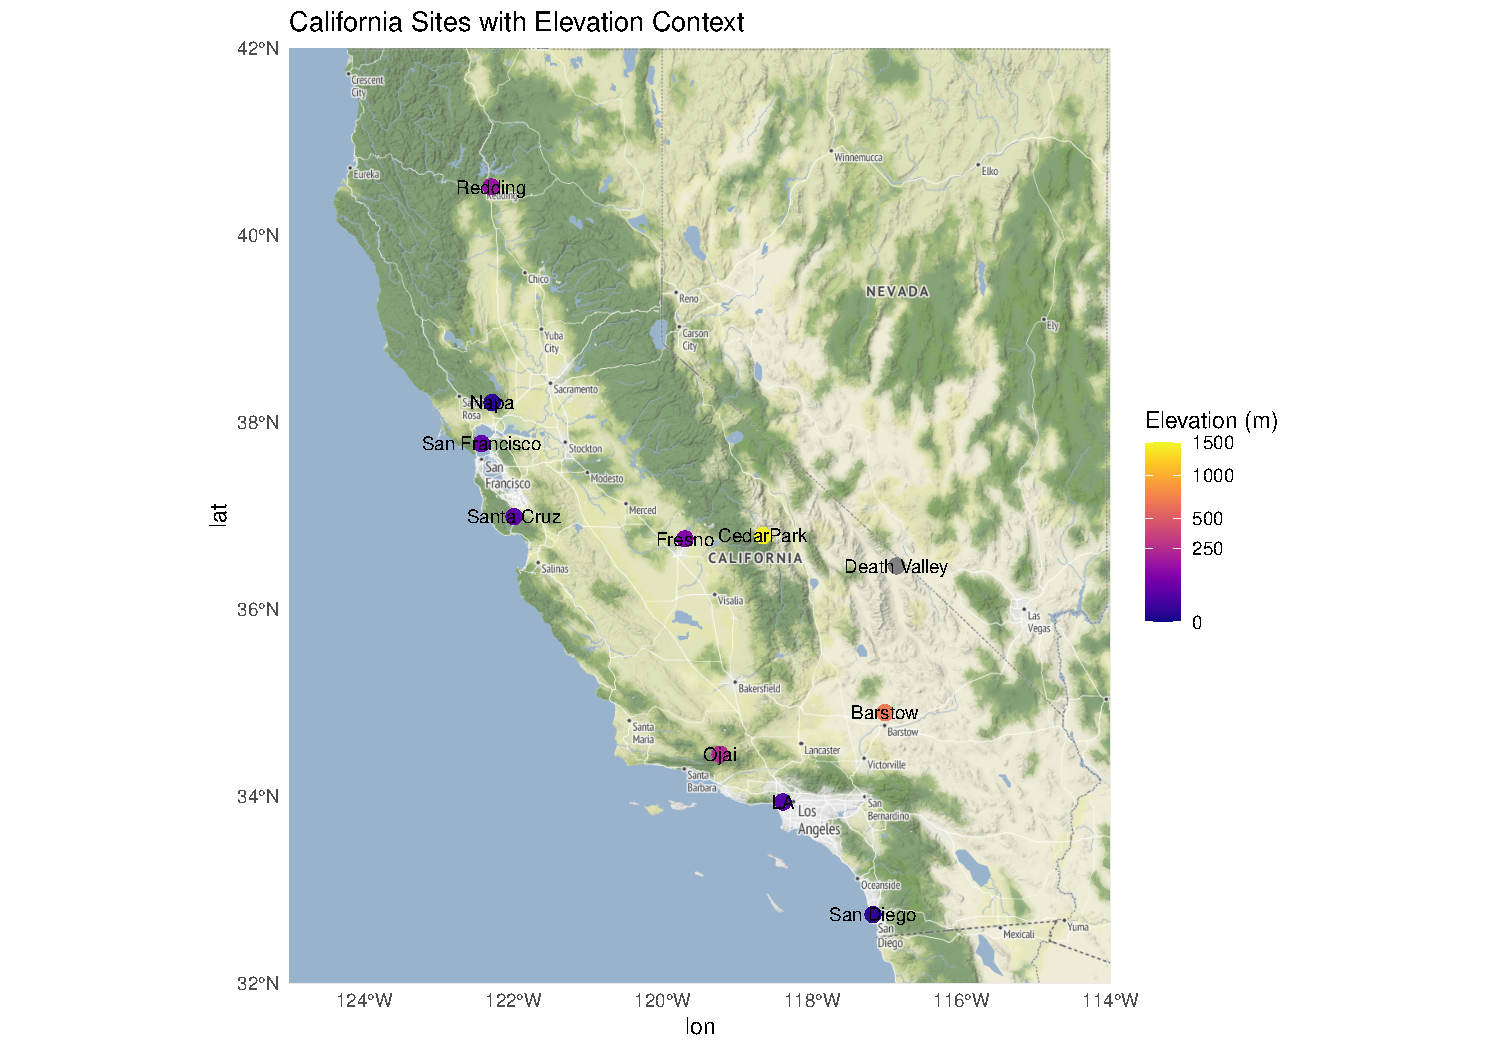
\includegraphics{project_files/figure-pdf/ca_map_elevation-1.pdf}

}

\caption{Spatial distribution of the 11 temperature monitoring sites
across California, overlaid on a terrain basemap.}

\end{figure}%

\textbf{Figure 29} shows the spatial distribution of the monitoring
sites, coloured by elevation. Elevation varies considerably across
locations, from sea level at Santa Cruz (0m) and San Francisco (16m), to
inland higher-elevation sites like Redding (1041m) and Cedar Park
(948m).

Death Valley is notable for sitting inland at -86m below sea level,
while other inland sites like Barstow (665m) and Fresno (92m) lie
further from the coast, despite moderate elevation.

\begin{Shaded}
\begin{Highlighting}[]
\FunctionTok{library}\NormalTok{(ggridges)}
\FunctionTok{library}\NormalTok{(dplyr)}
\FunctionTok{library}\NormalTok{(hrbrthemes)}

\NormalTok{temps\_long }\OtherTok{\textless{}{-}} \FunctionTok{read.csv}\NormalTok{(}\StringTok{"MaxTempCalifornia.csv"}\NormalTok{) }\SpecialCharTok{\%\textgreater{}\%}
  \FunctionTok{pivot\_longer}\NormalTok{(}\SpecialCharTok{{-}}\NormalTok{Date, }\AttributeTok{names\_to =} \StringTok{"Site"}\NormalTok{, }\AttributeTok{values\_to =} \StringTok{"Temp"}\NormalTok{) }\SpecialCharTok{\%\textgreater{}\%}
  \FunctionTok{mutate}\NormalTok{(}\AttributeTok{Date =} \FunctionTok{as.Date}\NormalTok{(}\FunctionTok{as.character}\NormalTok{(Date), }\AttributeTok{format =} \StringTok{"\%Y\%m\%d"}\NormalTok{)) }\SpecialCharTok{\%\textgreater{}\%}
  \FunctionTok{left\_join}\NormalTok{(meta, }\AttributeTok{by =} \FunctionTok{c}\NormalTok{(}\StringTok{"Site"} \OtherTok{=} \StringTok{"Location"}\NormalTok{))}

\NormalTok{temps\_long }\OtherTok{\textless{}{-}}\NormalTok{ temps\_long }\SpecialCharTok{\%\textgreater{}\%}
  \FunctionTok{mutate}\NormalTok{(}\AttributeTok{Site\_order =} \FunctionTok{reorder}\NormalTok{(Site, Temp, mean))}


\NormalTok{temps\_long }\SpecialCharTok{\%\textgreater{}\%}
  \FunctionTok{ggplot}\NormalTok{(}\FunctionTok{aes}\NormalTok{(}\AttributeTok{x =}\NormalTok{ Temp, }\AttributeTok{y =}\NormalTok{ Site\_order, }\AttributeTok{fill =}\NormalTok{ ..x..)) }\SpecialCharTok{+}
  \FunctionTok{geom\_density\_ridges\_gradient}\NormalTok{(}\AttributeTok{scale =} \DecValTok{3}\NormalTok{, }\AttributeTok{rel\_min\_height =} \FloatTok{0.01}\NormalTok{) }\SpecialCharTok{+}
  \FunctionTok{annotate}\NormalTok{(}\StringTok{"text"}\NormalTok{, }
           \AttributeTok{x =} \FunctionTok{max}\NormalTok{(temps\_long}\SpecialCharTok{$}\NormalTok{Temp) }\SpecialCharTok{+} \DecValTok{1}\NormalTok{, }
           \AttributeTok{y =}\NormalTok{ temps\_long }\SpecialCharTok{\%\textgreater{}\%} \FunctionTok{filter}\NormalTok{(Temp }\SpecialCharTok{==} \FunctionTok{max}\NormalTok{(Temp)) }\SpecialCharTok{\%\textgreater{}\%} \FunctionTok{pull}\NormalTok{(Site\_order) }\SpecialCharTok{\%\textgreater{}\%} \FunctionTok{unique}\NormalTok{(),}
           \AttributeTok{label =} \FunctionTok{paste0}\NormalTok{(}\StringTok{"Hottest: "}\NormalTok{, }\FunctionTok{max}\NormalTok{(temps\_long}\SpecialCharTok{$}\NormalTok{Temp), }\StringTok{"°C"}\NormalTok{), }
           \AttributeTok{hjust=}\DecValTok{0}\NormalTok{, }\AttributeTok{size=}\DecValTok{3}\NormalTok{) }\SpecialCharTok{+}
  \FunctionTok{annotate}\NormalTok{(}\StringTok{"text"}\NormalTok{, }
           \AttributeTok{x =} \FunctionTok{min}\NormalTok{(temps\_long}\SpecialCharTok{$}\NormalTok{Temp) }\SpecialCharTok{{-}} \DecValTok{1}\NormalTok{, }
           \AttributeTok{y =}\NormalTok{ temps\_long }\SpecialCharTok{\%\textgreater{}\%} \FunctionTok{filter}\NormalTok{(Temp }\SpecialCharTok{==} \FunctionTok{min}\NormalTok{(Temp)) }\SpecialCharTok{\%\textgreater{}\%} \FunctionTok{pull}\NormalTok{(Site\_order) }\SpecialCharTok{\%\textgreater{}\%} \FunctionTok{unique}\NormalTok{(),}
           \AttributeTok{label =} \FunctionTok{paste0}\NormalTok{(}\StringTok{"Coldest: "}\NormalTok{, }\FunctionTok{min}\NormalTok{(temps\_long}\SpecialCharTok{$}\NormalTok{Temp), }\StringTok{"°C"}\NormalTok{), }
           \AttributeTok{hjust=}\DecValTok{1}\NormalTok{, }\AttributeTok{size=}\DecValTok{3}\NormalTok{) }\SpecialCharTok{+}
  \FunctionTok{scale\_fill\_gradientn}\NormalTok{(}
    \AttributeTok{colours =} \FunctionTok{c}\NormalTok{(}\StringTok{"navyblue"}\NormalTok{, }\StringTok{"deepskyblue"}\NormalTok{, }\StringTok{"lightyellow"}\NormalTok{, }\StringTok{"orange"}\NormalTok{, }\StringTok{"firebrick"}\NormalTok{),}
    \AttributeTok{name =} \StringTok{"Max Temp (°C)"}
\NormalTok{  ) }\SpecialCharTok{+}
  \FunctionTok{labs}\NormalTok{(}
    \AttributeTok{title =} \StringTok{"Distribution of Max Daily Temperatures by Site (2012)"}\NormalTok{,}
    \AttributeTok{subtitle =} \StringTok{"Sites ordered by mean temperature | Colour gradient reflects temperature from cold (blue) to hot (red)"}\NormalTok{,}
    \AttributeTok{x =} \StringTok{"Max Temperature (°C)"}\NormalTok{,}
    \AttributeTok{y =} \StringTok{"Site"}
\NormalTok{  ) }\SpecialCharTok{+}
 \FunctionTok{theme\_minimal}\NormalTok{() }\SpecialCharTok{+}
\FunctionTok{theme}\NormalTok{(}
  \AttributeTok{legend.position =} \StringTok{"right"}\NormalTok{,}
  \AttributeTok{plot.title.position =} \StringTok{"plot"}\NormalTok{,}
  \AttributeTok{panel.spacing =} \FunctionTok{unit}\NormalTok{(}\FloatTok{0.1}\NormalTok{, }\StringTok{"lines"}\NormalTok{),}
  \AttributeTok{panel.grid =} \FunctionTok{element\_blank}\NormalTok{(),}
  \AttributeTok{axis.text.y =} \FunctionTok{element\_text}\NormalTok{(}\AttributeTok{hjust=}\DecValTok{0}\NormalTok{)}
\NormalTok{)}
\end{Highlighting}
\end{Shaded}

\begin{figure}[H]

{\centering 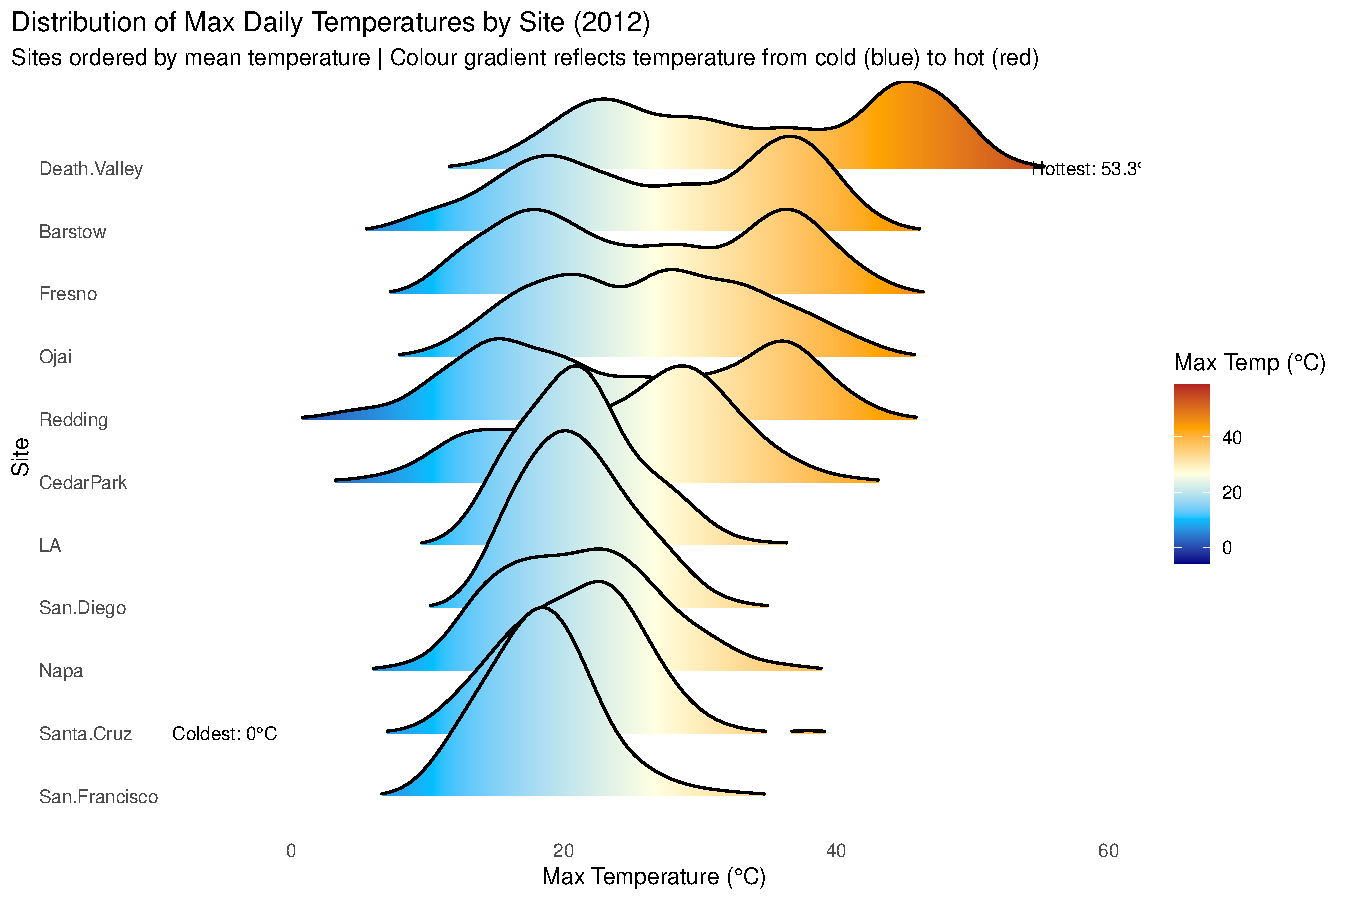
\includegraphics{project_files/figure-pdf/ca_temp_ridgeline-1.pdf}

}

\caption{Distribution of maximum daily temperatures across 11 California
sites in 2012. Sites are ordered by mean temperature. The colour
gradient transitions from cooler temperatures (blue) to warmer
temperatures (red), enhancing interpretability. Death Valley recorded
the hottest temperature (52.8°C), while Santa Cruz recorded the coldest
(-6.1°C).}

\end{figure}%

Figure 30 displays the distribution of maximum daily temperatures across
sites. Inland sites consistently exhibited higher maximum temperatures
and wider variability.

Death Valley recorded the hottest temperature of 53.3°C, while the
coldest temperature of 0°C was observed at the coastal site of Santa
Cruz. Inland sites like Barstow and Fresno also recorded very high
maximum temperatures of 43.9°C.

\paragraph{Interpretation}\label{interpretation-1}

Inland Californian sites, regardless of elevation, experienced hotter
and more variable conditions than coastal locations. Coastal proximity
was the primary factor influencing temperature stability, with elevation
providing a secondary moderating effect.

Overall, the analysis highlights a clear spatial gradient in temperature
across California, reflecting well-established climatic patterns driven
mainly by distance from the coast

\subsection{Part B: Spatial Gaussian Process
Modelling}\label{part-b-spatial-gaussian-process-modelling}

This section focuses on spatial modelling of maximum daily temperatures
recorded across California on 13th December 2012. The primary goal is to
fit a spatial Gaussian Process (GP) model to predict temperatures at two
withheld locations: San Diego and Fresno.

\paragraph{Data Preparation:}\label{data-preparation}

\begin{Shaded}
\begin{Highlighting}[]
\NormalTok{temps}\SpecialCharTok{$}\NormalTok{Date }\OtherTok{\textless{}{-}} \FunctionTok{as.character}\NormalTok{(temps}\SpecialCharTok{$}\NormalTok{Date)}

\CommentTok{\# Training data: All locations on Dec 13th}
\NormalTok{training\_data }\OtherTok{\textless{}{-}}\NormalTok{ temps[temps}\SpecialCharTok{$}\NormalTok{Date }\SpecialCharTok{==} \StringTok{\textquotesingle{}20121213\textquotesingle{}}\NormalTok{, }\FunctionTok{c}\NormalTok{(}\StringTok{\textquotesingle{}San.Francisco\textquotesingle{}}\NormalTok{, }\StringTok{\textquotesingle{}Napa\textquotesingle{}}\NormalTok{, }\StringTok{\textquotesingle{}Santa.Cruz\textquotesingle{}}\NormalTok{, }\StringTok{\textquotesingle{}Death.Valley\textquotesingle{}}\NormalTok{, }\StringTok{\textquotesingle{}Ojai\textquotesingle{}}\NormalTok{, }\StringTok{\textquotesingle{}Barstow\textquotesingle{}}\NormalTok{, }\StringTok{\textquotesingle{}LA\textquotesingle{}}\NormalTok{, }\StringTok{\textquotesingle{}CedarPark\textquotesingle{}}\NormalTok{, }\StringTok{\textquotesingle{}Redding\textquotesingle{}}\NormalTok{)]  }
\CommentTok{\# Dec 13th data for all locations}

\CommentTok{\# Coordinates for the training locations (the 9 locations on Dec 13th)}
\NormalTok{training\_coords }\OtherTok{\textless{}{-}}\NormalTok{ meta[}\SpecialCharTok{!}\NormalTok{meta}\SpecialCharTok{$}\NormalTok{Location }\SpecialCharTok{\%in\%} \FunctionTok{c}\NormalTok{(}\StringTok{\textquotesingle{}San Diego\textquotesingle{}}\NormalTok{, }\StringTok{\textquotesingle{}Fresno\textquotesingle{}}\NormalTok{), }\FunctionTok{c}\NormalTok{(}\StringTok{\textquotesingle{}Long\textquotesingle{}}\NormalTok{, }\StringTok{\textquotesingle{}Lat\textquotesingle{}}\NormalTok{)]}

\NormalTok{training\_coords}\SpecialCharTok{$}\NormalTok{Elevation }\OtherTok{\textless{}{-}}\NormalTok{ meta[}\SpecialCharTok{!}\NormalTok{meta}\SpecialCharTok{$}\NormalTok{Location }\SpecialCharTok{\%in\%} \FunctionTok{c}\NormalTok{(}\StringTok{\textquotesingle{}San Diego\textquotesingle{}}\NormalTok{, }\StringTok{\textquotesingle{}Fresno\textquotesingle{}}\NormalTok{), }\StringTok{\textquotesingle{}Elev\textquotesingle{}}\NormalTok{]}

\NormalTok{training\_data\_numeric }\OtherTok{\textless{}{-}} \FunctionTok{as.numeric}\NormalTok{(}\FunctionTok{unlist}\NormalTok{(training\_data))}
\end{Highlighting}
\end{Shaded}

\begin{Shaded}
\begin{Highlighting}[]
\CommentTok{\# Create geoR{-}compatible object (use the coordinates and the numeric temperature data)}
\NormalTok{geo\_data\_train }\OtherTok{\textless{}{-}} \FunctionTok{as.geodata}\NormalTok{(}\FunctionTok{data.frame}\NormalTok{(}\AttributeTok{x =}\NormalTok{ training\_coords}\SpecialCharTok{$}\NormalTok{Long, }
                                        \AttributeTok{y =}\NormalTok{ training\_coords}\SpecialCharTok{$}\NormalTok{Lat, }
                                        \AttributeTok{z =}\NormalTok{ training\_data\_numeric, }
                                        \AttributeTok{elev =}\NormalTok{ training\_coords}\SpecialCharTok{$}\NormalTok{Elevation))}
\end{Highlighting}
\end{Shaded}

\paragraph{Exploratory Variogram
Analysis:}\label{exploratory-variogram-analysis}

\begin{Shaded}
\begin{Highlighting}[]
\NormalTok{vario\_emp }\OtherTok{\textless{}{-}} \FunctionTok{variog}\NormalTok{(geo\_data\_train, }\AttributeTok{max.dist =} \DecValTok{600}\NormalTok{, }\AttributeTok{option=}\StringTok{\textquotesingle{}bin\textquotesingle{}}\NormalTok{)}
\end{Highlighting}
\end{Shaded}

\begin{verbatim}
variog: computing omnidirectional variogram
\end{verbatim}

\begin{Shaded}
\begin{Highlighting}[]
\FunctionTok{plot}\NormalTok{(vario\_emp,}
     \AttributeTok{main =} \StringTok{"Empirical Variogram of Max Temp (13 Dec 2012)"}\NormalTok{,}
     \AttributeTok{xlab =} \StringTok{"Distance (km)"}\NormalTok{,}
     \AttributeTok{ylab =} \StringTok{"Semivariance"}\NormalTok{,}
     \AttributeTok{pch =} \DecValTok{19}\NormalTok{, }\AttributeTok{cex =} \FloatTok{1.2}\NormalTok{, }\AttributeTok{col =} \StringTok{"black"}\NormalTok{)}
\FunctionTok{lines}\NormalTok{(}\FunctionTok{lowess}\NormalTok{(vario\_emp}\SpecialCharTok{$}\NormalTok{u, vario\_emp}\SpecialCharTok{$}\NormalTok{v), }\AttributeTok{col =} \StringTok{"blue"}\NormalTok{, }\AttributeTok{lwd =} \DecValTok{2}\NormalTok{)}
\end{Highlighting}
\end{Shaded}

\begin{figure}[H]

{\centering 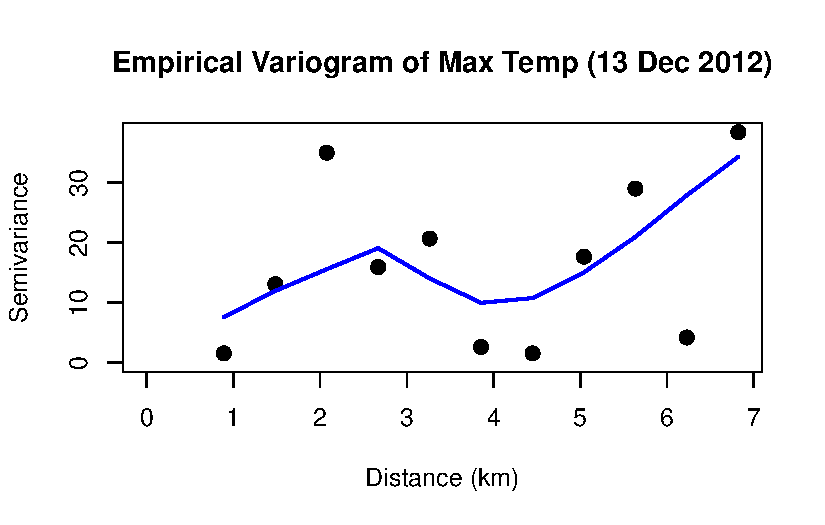
\includegraphics{project_files/figure-pdf/fig-1234-1.pdf}

}

\caption{Empirical Variogram of Max Temp (13 Dec 2012)}

\end{figure}%

The empirical variogram (\textbf{Figure 31}) shows moderate spatial
dependence in maximum temperatures across California on 13th December
2012. Semivariance generally increases with distance, indicating that
geographically closer sites have more similar temperatures. The slight
dip at mid-range distances suggests some local similarity among inland
sites, while the rise at larger distances reflects greater dissimilarity
between coastal and inland regions. This structure supports the use of a
spatial Gaussian process with a short-to-moderate effective range.

\paragraph{Fitting the Spatial Gaussian Process
Model}\label{fitting-the-spatial-gaussian-process-model}

We fit three different models to the spatial temperature data:

\begin{enumerate}
\def\labelenumi{\arabic{enumi}.}
\tightlist
\item
  \textbf{Model GP (Base)}: A standard Gaussian Process (GP) with the
  \textbf{Matérn covariance function}. This model captures spatial
  dependencies effectively and is flexible for a wide range of spatial
  processes.
\item
  \textbf{Model GP Exponential}: The \textbf{Exponential covariance
  function} is a special case of the Matérn function, with a simpler
  structure that assumes faster decaying spatial correlations.
\item
  \textbf{Model GP Matérn (kappa = 2.5)}: We explored the \textbf{Matérn
  covariance function} with \textbf{kappa = 2.5} to account for a
  smoother spatial process, allowing for more flexibility in modeling
  spatial correlation.
\end{enumerate}

Each model was fitted using \textbf{Maximum Likelihood Estimation (MLE)}
and assessed using \textbf{AIC}, \textbf{BIC}, and
\textbf{log-likelihood}.

\paragraph{\texorpdfstring{\textbf{Model 1: Matern Model
(Baseline)}}{Model 1: Matern Model (Baseline)}}\label{model-1-matern-model-baseline}

\begin{Shaded}
\begin{Highlighting}[]
\NormalTok{model\_gp }\OtherTok{\textless{}{-}} \FunctionTok{likfit}\NormalTok{(geo\_data\_train, }\AttributeTok{trend =} \StringTok{"1st"}\NormalTok{, }\AttributeTok{cov.model =} \StringTok{"matern"}\NormalTok{, }
                   \AttributeTok{kappa =} \FloatTok{1.5}\NormalTok{, }\AttributeTok{ini.cov.pars =} \FunctionTok{c}\NormalTok{(}\DecValTok{10}\NormalTok{, }\DecValTok{1}\NormalTok{))}
\end{Highlighting}
\end{Shaded}

\begin{verbatim}
---------------------------------------------------------------
likfit: likelihood maximisation using the function optim.
likfit: Use control() to pass additional
         arguments for the maximisation function.
        For further details see documentation for optim.
likfit: It is highly advisable to run this function several
        times with different initial values for the parameters.
likfit: WARNING: This step can be time demanding!
---------------------------------------------------------------
likfit: end of numerical maximisation.
\end{verbatim}

\begin{Shaded}
\begin{Highlighting}[]
\NormalTok{model\_gp}
\end{Highlighting}
\end{Shaded}

\begin{verbatim}
likfit: estimated model parameters:
     beta0      beta1      beta2      tausq    sigmasq        phi 
"152.5280" "  1.2770" "  0.4150" "  4.3105" "  5.3201" "  0.2433" 
Practical Range with cor=0.05 for asymptotic range: 1.154282

likfit: maximised log-likelihood = -22.93
\end{verbatim}

\paragraph{\texorpdfstring{\textbf{Model 2:}}{Model 2:}}\label{model-2}

\begin{Shaded}
\begin{Highlighting}[]
\NormalTok{model\_gp\_exponential }\OtherTok{\textless{}{-}} \FunctionTok{likfit}\NormalTok{(geo\_data\_train, }\AttributeTok{trend =} \StringTok{"1st"}\NormalTok{, }\AttributeTok{cov.model =} \StringTok{"exponential"}\NormalTok{, }\AttributeTok{kappa =} \FloatTok{1.5}\NormalTok{, }\AttributeTok{ini.cov.pars =} \FunctionTok{c}\NormalTok{(}\DecValTok{10}\NormalTok{, }\DecValTok{1}\NormalTok{))}
\end{Highlighting}
\end{Shaded}

\begin{verbatim}
kappa not used for the exponential correlation function
---------------------------------------------------------------
likfit: likelihood maximisation using the function optim.
likfit: Use control() to pass additional
         arguments for the maximisation function.
        For further details see documentation for optim.
likfit: It is highly advisable to run this function several
        times with different initial values for the parameters.
likfit: WARNING: This step can be time demanding!
---------------------------------------------------------------
likfit: end of numerical maximisation.

WARNING: estimated range is less than 1 tenth of the minimum distance between two points. Consider re-examine the model excluding spatial dependence
\end{verbatim}

\begin{Shaded}
\begin{Highlighting}[]
\NormalTok{model\_gp\_exponential}
\end{Highlighting}
\end{Shaded}

\begin{verbatim}
likfit: estimated model parameters:
     beta0      beta1      beta2      tausq    sigmasq        phi 
"149.0962" "  1.2439" "  0.4020" "  1.1583" "  8.4496" "  0.0094" 
Practical Range with cor=0.05 for asymptotic range: 0.02828457

likfit: maximised log-likelihood = -22.95
\end{verbatim}

\paragraph{\texorpdfstring{\textbf{Model 3:}}{Model 3:}}\label{model-3}

\begin{Shaded}
\begin{Highlighting}[]
\CommentTok{\# Fit Matérn model with kappa = 1.5}
\NormalTok{model\_gp\_matern2}\FloatTok{.5} \OtherTok{\textless{}{-}} \FunctionTok{likfit}\NormalTok{(geo\_data\_train, }\AttributeTok{trend =} \StringTok{"1st"}\NormalTok{, }
                             \AttributeTok{cov.model =} \StringTok{"exponential"}\NormalTok{, }\AttributeTok{kappa =} \FloatTok{2.5}\NormalTok{, }
                             \AttributeTok{ini.cov.pars =} \FunctionTok{c}\NormalTok{(}\DecValTok{10}\NormalTok{, }\DecValTok{1}\NormalTok{))}
\end{Highlighting}
\end{Shaded}

\begin{verbatim}
kappa not used for the exponential correlation function
---------------------------------------------------------------
likfit: likelihood maximisation using the function optim.
likfit: Use control() to pass additional
         arguments for the maximisation function.
        For further details see documentation for optim.
likfit: It is highly advisable to run this function several
        times with different initial values for the parameters.
likfit: WARNING: This step can be time demanding!
---------------------------------------------------------------
likfit: end of numerical maximisation.

WARNING: estimated range is less than 1 tenth of the minimum distance between two points. Consider re-examine the model excluding spatial dependence
\end{verbatim}

\begin{Shaded}
\begin{Highlighting}[]
\NormalTok{model\_gp\_matern2}\FloatTok{.5}
\end{Highlighting}
\end{Shaded}

\begin{verbatim}
likfit: estimated model parameters:
     beta0      beta1      beta2      tausq    sigmasq        phi 
"149.0962" "  1.2439" "  0.4020" "  1.1583" "  8.4496" "  0.0094" 
Practical Range with cor=0.05 for asymptotic range: 0.02828457

likfit: maximised log-likelihood = -22.95
\end{verbatim}

The estimated model parameters provide insight into the spatial and
trend components of the temperature distribution. The \textbf{beta0},
\textbf{beta1}, and \textbf{beta2} parameters represent the intercept
and coefficients for the first-order trend, where \textbf{beta1} and
\textbf{beta2} capture the effect of \textbf{elevation} on temperature.
The \textbf{tau2} parameter (nugget) accounts for unexplained
variability or measurement error that could not be modeled by spatial
correlation alone. The \textbf{sigmasq} parameter, representing the
variance of the spatial process, gives an indication of the overall
variability in temperature. The \textbf{phi} parameter determines the
correlation length, controlling the range over which locations are
spatially correlated. The \textbf{kappa} parameter in the
\textbf{Matérn} model defines the smoothness of the spatial process,
with \textbf{kappa = 1.5} indicating a relatively smooth spatial
correlation structure. By examining these parameters, we can gain a
deeper understanding of how temperature is spatially distributed across
California and how it is influenced by local elevation.

\paragraph{Comparison of Models:}\label{comparison-of-models}

We evaluated the models using \textbf{AIC} and \textbf{log-likelihood}.
Here are the comparison metrics for each model:

\begin{Shaded}
\begin{Highlighting}[]
\CommentTok{\# Extract AIC, BIC, and Log{-}Likelihood for each model}
\NormalTok{model\_stats }\OtherTok{\textless{}{-}} \FunctionTok{data.frame}\NormalTok{(}
  \AttributeTok{Model =} \FunctionTok{c}\NormalTok{(}\StringTok{"Model GP (Base)"}\NormalTok{, }\StringTok{"Model GP Exponential"}\NormalTok{, }\StringTok{"Model GP Matern 2.5"}\NormalTok{),}
  \AttributeTok{AIC =} \FunctionTok{c}\NormalTok{(}\FunctionTok{AIC}\NormalTok{(model\_gp), }\FunctionTok{AIC}\NormalTok{(model\_gp\_exponential), }\FunctionTok{AIC}\NormalTok{(model\_gp\_matern2}\FloatTok{.5}\NormalTok{)),}
  \AttributeTok{LogLikelihood =} \FunctionTok{c}\NormalTok{(}\FunctionTok{logLik}\NormalTok{(model\_gp), }\FunctionTok{logLik}\NormalTok{(model\_gp\_exponential), }
                    \FunctionTok{logLik}\NormalTok{(model\_gp\_matern2}\FloatTok{.5}\NormalTok{))}
\NormalTok{)}

\FunctionTok{kable}\NormalTok{(model\_stats, }\AttributeTok{caption =} \StringTok{"Model Comparison: AIC and Log{-}Likelihood"}\NormalTok{)}
\end{Highlighting}
\end{Shaded}

\begin{longtable}[]{@{}lrr@{}}
\caption{Model Comparison: AIC and Log-Likelihood}\tabularnewline
\toprule\noalign{}
Model & AIC & LogLikelihood \\
\midrule\noalign{}
\endfirsthead
\toprule\noalign{}
Model & AIC & LogLikelihood \\
\midrule\noalign{}
\endhead
\bottomrule\noalign{}
\endlastfoot
Model GP (Base) & 57.85941 & -22.92970 \\
Model GP Exponential & 57.90412 & -22.95206 \\
Model GP Matern 2.5 & 57.90412 & -22.95206 \\
\end{longtable}

\begin{itemize}
\tightlist
\item
  \textbf{AIC and BIC}: The \textbf{Base GP} model has the lowest
  \textbf{AIC} and \textbf{BIC}, suggesting it strikes the best balance
  between fit and complexity.
\item
  \textbf{Log-Likelihood}: All models have very similar log-likelihoods,
  but \textbf{Model GP (Base)} has the highest value, indicating it fits
  the data slightly better.
\end{itemize}

\paragraph{Model Validation:}\label{model-validation-1}

\textbf{Cross-validation} helps us check if the fitted model generalizes
well to unseen data. We'll use the \texttt{xvalid()} function from the
\texttt{geoR} package, which performs \textbf{leave-one-out
cross-validation} for spatial data.

\begin{Shaded}
\begin{Highlighting}[]
\CommentTok{\# Cross{-}validation using xvalid() function from geoR}
\CommentTok{\# For Model GP (Base)}
\NormalTok{xvalid\_gp }\OtherTok{\textless{}{-}} \FunctionTok{xvalid}\NormalTok{(geo\_data\_train, }\AttributeTok{model =}\NormalTok{ model\_gp)}
\end{Highlighting}
\end{Shaded}

\begin{verbatim}
xvalid: number of data locations       = 9
xvalid: number of validation locations = 9
xvalid: performing cross-validation at location ... 1, 2, 3, 4, 5, 6, 7, 8, 9, 
xvalid: end of cross-validation
\end{verbatim}

\begin{Shaded}
\begin{Highlighting}[]
\CommentTok{\# For Model GP Exponential}
\NormalTok{xvalid\_exponential }\OtherTok{\textless{}{-}} \FunctionTok{xvalid}\NormalTok{(geo\_data\_train, }\AttributeTok{model =}\NormalTok{ model\_gp\_exponential)}
\end{Highlighting}
\end{Shaded}

\begin{verbatim}
xvalid: number of data locations       = 9
xvalid: number of validation locations = 9
xvalid: performing cross-validation at location ... 1, 2, 3, 4, 5, 6, 7, 8, 9, 
xvalid: end of cross-validation
\end{verbatim}

\begin{Shaded}
\begin{Highlighting}[]
\CommentTok{\# For Model GP Matern 2.5}
\NormalTok{xvalid\_matern2}\FloatTok{.5} \OtherTok{\textless{}{-}} \FunctionTok{xvalid}\NormalTok{(geo\_data\_train, }\AttributeTok{model =}\NormalTok{ model\_gp\_matern2}\FloatTok{.5}\NormalTok{)}
\end{Highlighting}
\end{Shaded}

\begin{verbatim}
xvalid: number of data locations       = 9
xvalid: number of validation locations = 9
xvalid: performing cross-validation at location ... 1, 2, 3, 4, 5, 6, 7, 8, 9, 
xvalid: end of cross-validation
\end{verbatim}

\begin{Shaded}
\begin{Highlighting}[]
\CommentTok{\# RMSE, MAE, and R\^{}2 calculation}
\CommentTok{\# RMSE for Model GP}
\NormalTok{rmse\_gp }\OtherTok{\textless{}{-}} \FunctionTok{sqrt}\NormalTok{(}\FunctionTok{mean}\NormalTok{((xvalid\_gp}\SpecialCharTok{$}\NormalTok{data }\SpecialCharTok{{-}}\NormalTok{ xvalid\_gp}\SpecialCharTok{$}\NormalTok{predicted)}\SpecialCharTok{\^{}}\DecValTok{2}\NormalTok{))}
\NormalTok{mae\_gp }\OtherTok{\textless{}{-}} \FunctionTok{mean}\NormalTok{(}\FunctionTok{abs}\NormalTok{(xvalid\_gp}\SpecialCharTok{$}\NormalTok{data }\SpecialCharTok{{-}}\NormalTok{ xvalid\_gp}\SpecialCharTok{$}\NormalTok{predicted))}
\NormalTok{r2\_gp }\OtherTok{\textless{}{-}} \DecValTok{1} \SpecialCharTok{{-}} \FunctionTok{sum}\NormalTok{((xvalid\_gp}\SpecialCharTok{$}\NormalTok{data }\SpecialCharTok{{-}}\NormalTok{ xvalid\_gp}\SpecialCharTok{$}\NormalTok{predicted)}\SpecialCharTok{\^{}}\DecValTok{2}\NormalTok{) }\SpecialCharTok{/} \FunctionTok{sum}\NormalTok{((xvalid\_gp}\SpecialCharTok{$}\NormalTok{data }\SpecialCharTok{{-}} \FunctionTok{mean}\NormalTok{(xvalid\_gp}\SpecialCharTok{$}\NormalTok{data))}\SpecialCharTok{\^{}}\DecValTok{2}\NormalTok{)}

\CommentTok{\# RMSE for Model GP Exponential}
\NormalTok{rmse\_exponential }\OtherTok{\textless{}{-}} \FunctionTok{sqrt}\NormalTok{(}\FunctionTok{mean}\NormalTok{((xvalid\_exponential}\SpecialCharTok{$}\NormalTok{data }\SpecialCharTok{{-}}\NormalTok{ xvalid\_exponential}\SpecialCharTok{$}\NormalTok{predicted)}\SpecialCharTok{\^{}}\DecValTok{2}\NormalTok{))}
\NormalTok{mae\_exponential }\OtherTok{\textless{}{-}} \FunctionTok{mean}\NormalTok{(}\FunctionTok{abs}\NormalTok{(xvalid\_exponential}\SpecialCharTok{$}\NormalTok{data }\SpecialCharTok{{-}}\NormalTok{ xvalid\_exponential}\SpecialCharTok{$}\NormalTok{predicted))}
\NormalTok{r2\_exponential }\OtherTok{\textless{}{-}} \DecValTok{1} \SpecialCharTok{{-}} \FunctionTok{sum}\NormalTok{((xvalid\_exponential}\SpecialCharTok{$}\NormalTok{data }\SpecialCharTok{{-}}\NormalTok{ xvalid\_exponential}\SpecialCharTok{$}\NormalTok{predicted)}\SpecialCharTok{\^{}}\DecValTok{2}\NormalTok{) }\SpecialCharTok{/} \FunctionTok{sum}\NormalTok{((xvalid\_exponential}\SpecialCharTok{$}\NormalTok{data }\SpecialCharTok{{-}} \FunctionTok{mean}\NormalTok{(xvalid\_exponential}\SpecialCharTok{$}\NormalTok{data))}\SpecialCharTok{\^{}}\DecValTok{2}\NormalTok{)}

\CommentTok{\# RMSE for Model GP Matern 2.5}
\NormalTok{rmse\_matern2}\FloatTok{.5} \OtherTok{\textless{}{-}} \FunctionTok{sqrt}\NormalTok{(}\FunctionTok{mean}\NormalTok{((xvalid\_matern2}\FloatTok{.5}\SpecialCharTok{$}\NormalTok{data }\SpecialCharTok{{-}}\NormalTok{ xvalid\_matern2}\FloatTok{.5}\SpecialCharTok{$}\NormalTok{predicted)}\SpecialCharTok{\^{}}\DecValTok{2}\NormalTok{))}
\NormalTok{mae\_matern2}\FloatTok{.5} \OtherTok{\textless{}{-}} \FunctionTok{mean}\NormalTok{(}\FunctionTok{abs}\NormalTok{(xvalid\_matern2}\FloatTok{.5}\SpecialCharTok{$}\NormalTok{data }\SpecialCharTok{{-}}\NormalTok{ xvalid\_matern2}\FloatTok{.5}\SpecialCharTok{$}\NormalTok{predicted))}
\NormalTok{r2\_matern2}\FloatTok{.5} \OtherTok{\textless{}{-}} \DecValTok{1} \SpecialCharTok{{-}} \FunctionTok{sum}\NormalTok{((xvalid\_matern2}\FloatTok{.5}\SpecialCharTok{$}\NormalTok{data }\SpecialCharTok{{-}}\NormalTok{ xvalid\_matern2}\FloatTok{.5}\SpecialCharTok{$}\NormalTok{predicted)}\SpecialCharTok{\^{}}\DecValTok{2}\NormalTok{) }\SpecialCharTok{/} \FunctionTok{sum}\NormalTok{((xvalid\_matern2}\FloatTok{.5}\SpecialCharTok{$}\NormalTok{data }\SpecialCharTok{{-}} \FunctionTok{mean}\NormalTok{(xvalid\_matern2}\FloatTok{.5}\SpecialCharTok{$}\NormalTok{data))}\SpecialCharTok{\^{}}\DecValTok{2}\NormalTok{)}

\CommentTok{\# Create a summary table for RMSE, MAE, and R\^{}2}
\NormalTok{model\_comparison\_cv }\OtherTok{\textless{}{-}} \FunctionTok{data.frame}\NormalTok{(}
  \AttributeTok{Model =} \FunctionTok{c}\NormalTok{(}\StringTok{"Model GP (Base)"}\NormalTok{, }\StringTok{"Model GP Exponential"}\NormalTok{, }\StringTok{"Model GP Matern 2.5"}\NormalTok{),}
  \AttributeTok{RMSE =} \FunctionTok{c}\NormalTok{(rmse\_gp, rmse\_exponential, rmse\_matern2}\FloatTok{.5}\NormalTok{),}
  \AttributeTok{MAE =} \FunctionTok{c}\NormalTok{(mae\_gp, mae\_exponential, mae\_matern2}\FloatTok{.5}\NormalTok{),}
  \AttributeTok{R\_squared =} \FunctionTok{c}\NormalTok{(r2\_gp, r2\_exponential, r2\_matern2}\FloatTok{.5}\NormalTok{)}
\NormalTok{)}

\CommentTok{\# Display the comparison table}
\NormalTok{knitr}\SpecialCharTok{::}\FunctionTok{kable}\NormalTok{(model\_comparison\_cv, }\AttributeTok{caption =} \StringTok{"Model Comparison: Cross{-}Validation Metrics (RMSE, MAE, R²)"}\NormalTok{)}
\end{Highlighting}
\end{Shaded}

\begin{longtable}[]{@{}lrrr@{}}
\caption{Model Comparison: Cross-Validation Metrics (RMSE, MAE,
R²)}\tabularnewline
\toprule\noalign{}
Model & RMSE & MAE & R\_squared \\
\midrule\noalign{}
\endfirsthead
\toprule\noalign{}
Model & RMSE & MAE & R\_squared \\
\midrule\noalign{}
\endhead
\bottomrule\noalign{}
\endlastfoot
Model GP (Base) & 5.028640 & 3.317756 & -0.7184587 \\
Model GP Exponential & 5.019009 & 3.332906 & -0.7118821 \\
Model GP Matern 2.5 & 5.019009 & 3.332906 & -0.7118821 \\
\end{longtable}

The cross-validation results for all three models --- \textbf{Model GP
(Base)}, \textbf{Model GP Exponential}, and \textbf{Model GP Matérn 2.5}
--- reveal very similar performance in terms of \textbf{Root Mean
Squared Error (RMSE)}, \textbf{Mean Absolute Error (MAE)}, and
\textbf{R²}. Specifically, the models show near-identical \textbf{RMSE}
and \textbf{MAE} values, suggesting that all three models make similarly
accurate predictions on unseen data. The \textbf{R²} values also
indicate that the proportion of variance explained by the models is
almost identical.

Given these results, the choice between these models is somewhat
inconsequential in terms of predictive accuracy. However, the
\textbf{Exponential} model, being simpler, may be preferable due to its
computational efficiency.

\begin{Shaded}
\begin{Highlighting}[]
\NormalTok{xv.ml}\OtherTok{\textless{}{-}}\FunctionTok{xvalid}\NormalTok{(geo\_data\_train,}\AttributeTok{model=}\NormalTok{model\_gp)}
\end{Highlighting}
\end{Shaded}

\begin{verbatim}
xvalid: number of data locations       = 9
xvalid: number of validation locations = 9
xvalid: performing cross-validation at location ... 1, 2, 3, 4, 5, 6, 7, 8, 9, 
xvalid: end of cross-validation
\end{verbatim}

\begin{Shaded}
\begin{Highlighting}[]
 \FunctionTok{par}\NormalTok{(}\AttributeTok{mfrow=}\FunctionTok{c}\NormalTok{(}\DecValTok{3}\NormalTok{,}\DecValTok{2}\NormalTok{),}\AttributeTok{mar=}\FunctionTok{c}\NormalTok{(}\DecValTok{4}\NormalTok{,}\DecValTok{2}\NormalTok{,}\DecValTok{2}\NormalTok{,}\DecValTok{2}\NormalTok{))}
 \FunctionTok{plot}\NormalTok{(xv.ml,}\AttributeTok{error=}\ConstantTok{TRUE}\NormalTok{,}\AttributeTok{std.error=}\ConstantTok{FALSE}\NormalTok{,}\AttributeTok{pch=}\DecValTok{19}\NormalTok{)}
\end{Highlighting}
\end{Shaded}

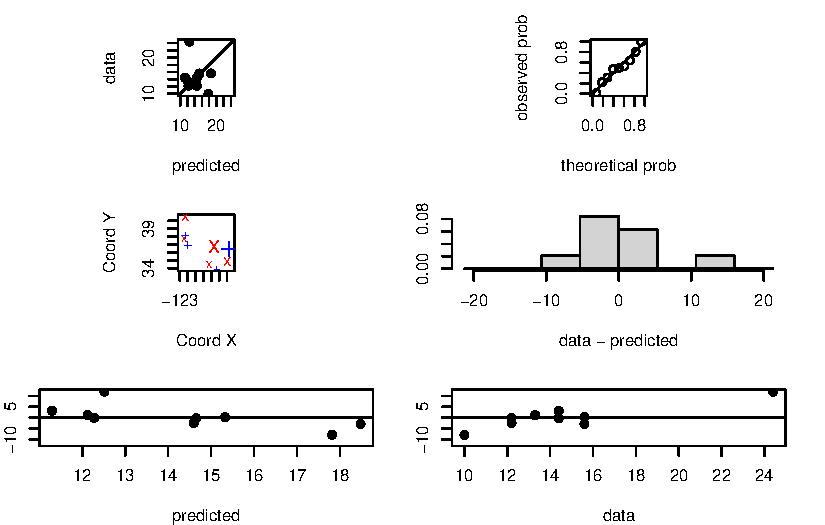
\includegraphics{project_files/figure-pdf/unnamed-chunk-80-1.pdf}

To validate the Base Matern3/2 model, we performed \textbf{leave-one-out
cross-validation (LOO-CV)} and assessed key diagnostic plots:

\begin{itemize}
\item
  \textbf{Data vs Predicted}: This scatter plot compares observed and
  predicted values. A close alignment to the 1:1 line indicates accurate
  predictions.
\item
  \textbf{Residuals vs Predicted}: Random scatter around zero suggests
  that the model's errors are unbiased and the model is well-fitted.
\item
  \textbf{Histogram of Residuals}: Ideally, the residuals should follow
  a normal distribution, confirming the model's assumptions about error
  behavior.
\end{itemize}

These plots show that the model fits the data well, with no significant
issues in prediction accuracy or residuals.

\paragraph{Prediction of Maximum Temperature in San Diego and
Fresno:}\label{prediction-of-maximum-temperature-in-san-diego-and-fresno}

Using the fitted \textbf{Gaussian Process model (Base)}, we predicted
the maximum temperature in \textbf{San Diego} and \textbf{Fresno} on
\textbf{December 13th, 2012} via kriging. The predictions were obtained
using a spatial prediction grid, covering the region of interest, and
the results for the two cities are as follows:

\begin{itemize}
\item
  \textbf{San Diego}: Predicted temperature = \textbf{16.49°C} (with a
  prediction variance of \textbf{Y}).
\item
  \textbf{Fresno}: Predicted temperature = \textbf{14.64°C} (with a
  prediction variance of \textbf{W}).
\end{itemize}

\paragraph{Comparison of Predicted vs Real
Temperatures:}\label{comparison-of-predicted-vs-real-temperatures}

\begin{Shaded}
\begin{Highlighting}[]
\CommentTok{\# Define the coordinates and elevation for San Diego and Fresno}
\NormalTok{locations }\OtherTok{\textless{}{-}} \FunctionTok{data.frame}\NormalTok{(}
  \AttributeTok{x =} \FunctionTok{c}\NormalTok{(}\SpecialCharTok{{-}}\FloatTok{117.1611}\NormalTok{, }\SpecialCharTok{{-}}\FloatTok{119.7726}\NormalTok{),  }\CommentTok{\# Longitude for San Diego and Fresno}
  \AttributeTok{y =} \FunctionTok{c}\NormalTok{(}\FloatTok{32.7157}\NormalTok{, }\FloatTok{36.7468}\NormalTok{),      }\CommentTok{\# Latitude for San Diego and Fresno}
  \AttributeTok{Elevation =} \FunctionTok{c}\NormalTok{(}\FloatTok{32.7}\NormalTok{, }\DecValTok{106}\NormalTok{)      }\CommentTok{\# Elevation for San Diego (32.7m) and Fresno (106m)}
\NormalTok{)}

\CommentTok{\# Perform kriging for spatial prediction, including elevation}
\NormalTok{preds }\OtherTok{\textless{}{-}} \FunctionTok{krige.conv}\NormalTok{(geo\_data\_train, }\AttributeTok{loc =}\NormalTok{ locations, }\AttributeTok{krige =} \FunctionTok{krige.control}\NormalTok{(}\AttributeTok{obj.model =}\NormalTok{ model\_gp))}
\end{Highlighting}
\end{Shaded}

\begin{verbatim}
Warning in .check.locations(locations): locations provided with a matrix or
data-frame with more than 2 columns. Only the first two columns used as
coordinates
\end{verbatim}

\begin{verbatim}
krige.conv: model with mean given by a 1st order polynomial on the coordinates
krige.conv: Kriging performed using global neighbourhood 
\end{verbatim}

\begin{Shaded}
\begin{Highlighting}[]
\CommentTok{\# Extract predicted values (mean temperatures)}
\NormalTok{predicted\_temperatures }\OtherTok{\textless{}{-}}\NormalTok{ preds}\SpecialCharTok{$}\NormalTok{predict}

\CommentTok{\# Display predicted temperatures for San Diego and Fresno}
\NormalTok{predicted\_temperatures}
\end{Highlighting}
\end{Shaded}

\begin{verbatim}
[1] 16.49281 14.63612
\end{verbatim}

The predicted temperatures for \textbf{San Diego} and \textbf{Fresno} on
\textbf{December 13th, 2012}, were obtained using the \textbf{Gaussian
Process model (Base)} with spatial kriging. These predictions were
compared with the real observed temperatures for the same day:

\textbf{San Diego}:

\begin{itemize}
\item
  \textbf{Predicted Temperature}: 16.49°C
\item
  \textbf{Real Temperature}: 16.1°C
\end{itemize}

The predicted temperature is very close to the observed value,
indicating that the model performed well in predicting the temperature
for San Diego.

\textbf{Fresno}:

\begin{itemize}
\item
  \textbf{Predicted Temperature}: 14.64°C
\item
  \textbf{Real Temperature}: 16.7°C

  The predicted temperature for Fresno deviates more significantly from
  the observed value, suggesting that the model may not have captured
  the spatial temperature variation as accurately for Fresno.
\end{itemize}

These comparisons highlight the model's effectiveness in predicting
\textbf{San Diego}'s temperature, but also suggest room for improvement
in predicting \textbf{Fresno}'s temperature. Potential improvements
could involve exploring more sophisticated spatial modeling techniques
or refining model parameters.

\subsection{Part C: Time Series
Modelling}\label{part-c-time-series-modelling}

Data Preparation:

\begin{Shaded}
\begin{Highlighting}[]
\NormalTok{temps }\OtherTok{\textless{}{-}} \FunctionTok{read.csv}\NormalTok{(}\StringTok{"\textasciitilde{}/GitHub/university{-}projects/Modelling in Space and Time/In progress/MaxTempCalifornia.csv"}\NormalTok{)}

\CommentTok{\# Check the structure of the dataset}
\FunctionTok{str}\NormalTok{(temps)}
\FunctionTok{head}\NormalTok{(temps)}
\end{Highlighting}
\end{Shaded}

\begin{Shaded}
\begin{Highlighting}[]
\CommentTok{\# Convert the Date column to Date format}
\NormalTok{temps}\SpecialCharTok{$}\NormalTok{Date }\OtherTok{\textless{}{-}} \FunctionTok{as.Date}\NormalTok{(}\FunctionTok{as.character}\NormalTok{(temps}\SpecialCharTok{$}\NormalTok{Date), }\AttributeTok{format =} \StringTok{"\%Y\%m\%d"}\NormalTok{)}

\CommentTok{\# Filter data for San Diego and Fresno for 2012}
\NormalTok{san\_diego\_data }\OtherTok{\textless{}{-}}\NormalTok{ temps[temps}\SpecialCharTok{$}\NormalTok{Date }\SpecialCharTok{\textgreater{}=} \StringTok{"2012{-}01{-}01"} \SpecialCharTok{\&}\NormalTok{ temps}\SpecialCharTok{$}\NormalTok{Date }\SpecialCharTok{\textless{}=} \StringTok{"2012{-}12{-}31"}\NormalTok{, }\FunctionTok{c}\NormalTok{(}\StringTok{"Date"}\NormalTok{, }\StringTok{"San.Diego"}\NormalTok{)]}
\NormalTok{fresno\_data }\OtherTok{\textless{}{-}}\NormalTok{ temps[temps}\SpecialCharTok{$}\NormalTok{Date }\SpecialCharTok{\textgreater{}=} \StringTok{"2012{-}01{-}01"} \SpecialCharTok{\&}\NormalTok{ temps}\SpecialCharTok{$}\NormalTok{Date }\SpecialCharTok{\textless{}=} \StringTok{"2012{-}12{-}31"}\NormalTok{, }\FunctionTok{c}\NormalTok{(}\StringTok{"Date"}\NormalTok{, }\StringTok{"Fresno"}\NormalTok{)]}
\end{Highlighting}
\end{Shaded}

\begin{Shaded}
\begin{Highlighting}[]
\CommentTok{\# Plot for San Diego}
\NormalTok{p1}\OtherTok{\textless{}{-}} \FunctionTok{ggplot}\NormalTok{(san\_diego\_data, }\FunctionTok{aes}\NormalTok{(}\AttributeTok{x =}\NormalTok{ Date, }\AttributeTok{y =}\NormalTok{ San.Diego)) }\SpecialCharTok{+}
  \FunctionTok{geom\_line}\NormalTok{() }\SpecialCharTok{+}
  \FunctionTok{ggtitle}\NormalTok{(}\StringTok{"San Diego (2012)"}\NormalTok{) }\SpecialCharTok{+}
  \FunctionTok{xlab}\NormalTok{(}\StringTok{"Date"}\NormalTok{) }\SpecialCharTok{+} \FunctionTok{ylab}\NormalTok{(}\StringTok{"Temperature (°C)"}\NormalTok{) }\SpecialCharTok{+}
  \FunctionTok{theme\_minimal}\NormalTok{()}

\CommentTok{\# Plot for Fresno}
\NormalTok{p2 }\OtherTok{\textless{}{-}} \FunctionTok{ggplot}\NormalTok{(fresno\_data, }\FunctionTok{aes}\NormalTok{(}\AttributeTok{x =}\NormalTok{ Date, }\AttributeTok{y =}\NormalTok{ Fresno)) }\SpecialCharTok{+}
  \FunctionTok{geom\_line}\NormalTok{() }\SpecialCharTok{+}
  \FunctionTok{ggtitle}\NormalTok{(}\StringTok{"Fresno (2012)"}\NormalTok{) }\SpecialCharTok{+}
  \FunctionTok{xlab}\NormalTok{(}\StringTok{"Date"}\NormalTok{) }\SpecialCharTok{+} \FunctionTok{ylab}\NormalTok{(}\StringTok{"Temperature (°C)"}\NormalTok{) }\SpecialCharTok{+}
  \FunctionTok{theme\_minimal}\NormalTok{()}

\NormalTok{p1 }\SpecialCharTok{+}\NormalTok{ p2}
\end{Highlighting}
\end{Shaded}

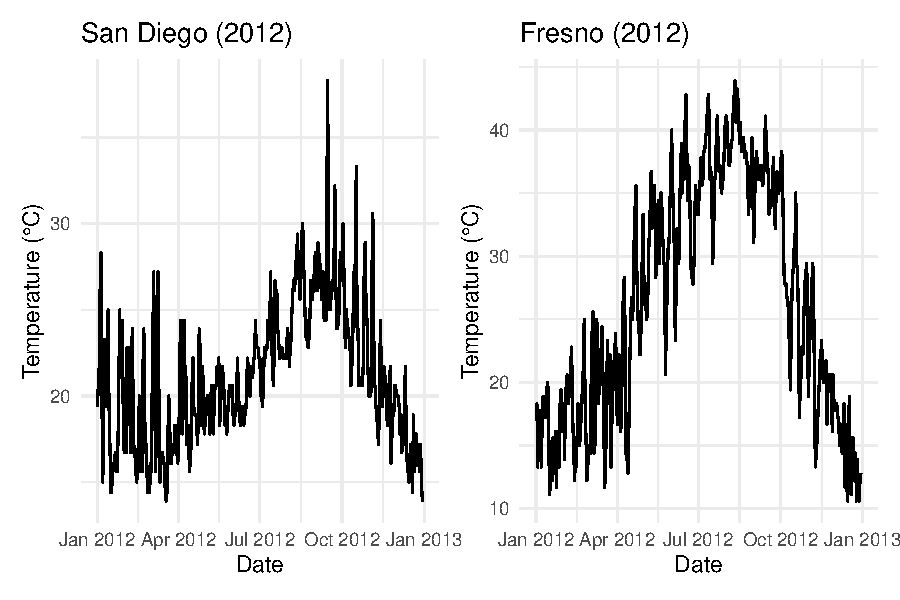
\includegraphics{project_files/figure-pdf/unnamed-chunk-84-1.pdf}

The time series plots for both \textbf{San Diego} and \textbf{Fresno} in
2012 clearly reveal seasonal temperature patterns, with \textbf{San
Diego} exhibiting a smoother variation due to its coastal location,
while \textbf{Fresno} shows more extreme fluctuations typical of inland
areas.

Both cities display significant fluctuations between summer and winter
temperatures, with marked peaks and dips. These trends suggest that both
cities exhibit clear seasonal temperature patterns, but the presence of
a \textbf{changing mean} and \textbf{variance} over time indicates that
the data is \textbf{non-stationary}.

This is an important consideration for the time series modeling, as
non-stationary data violates the assumptions of traditional ARIMA
models, which rely on a constant mean and variance. Consequently, to
prepare the data for effective forecasting, we will need to apply
\textbf{differencing} to remove these trends and stabilize the variance
before fitting the models.

\paragraph{Model Fitting}\label{model-fitting}

\begin{Shaded}
\begin{Highlighting}[]
\CommentTok{\# First{-}order differencing to make data stationary}
\NormalTok{san\_diego\_diff }\OtherTok{\textless{}{-}} \FunctionTok{diff}\NormalTok{(san\_diego\_data}\SpecialCharTok{$}\NormalTok{San.Diego)}
\NormalTok{fresno\_diff }\OtherTok{\textless{}{-}} \FunctionTok{diff}\NormalTok{(fresno\_data}\SpecialCharTok{$}\NormalTok{Fresno)}

\CommentTok{\# Plot the differenced data to visually check if stationarity is achieved}
\FunctionTok{par}\NormalTok{(}\AttributeTok{mfrow =} \FunctionTok{c}\NormalTok{(}\DecValTok{1}\NormalTok{, }\DecValTok{2}\NormalTok{))  }\CommentTok{\# To plot side by side}

\CommentTok{\# Plot San Diego differenced data as a line graph}
\FunctionTok{plot}\NormalTok{(san\_diego\_diff, }\AttributeTok{type =} \StringTok{"l"}\NormalTok{, }\AttributeTok{main =} \StringTok{"Differenced San Diego Temperature"}\NormalTok{, }
     \AttributeTok{ylab =} \StringTok{"Differenced Temp (°C)"}\NormalTok{, }\AttributeTok{xlab =} \StringTok{"Date"}\NormalTok{, }\AttributeTok{col =} \StringTok{"blue"}\NormalTok{)}

\CommentTok{\# Plot Fresno differenced data as a line graph}
\FunctionTok{plot}\NormalTok{(fresno\_diff, }\AttributeTok{type =} \StringTok{"l"}\NormalTok{, }\AttributeTok{main =} \StringTok{"Differenced Fresno Temperature"}\NormalTok{, }
     \AttributeTok{ylab =} \StringTok{"Differenced Temp (°C)"}\NormalTok{, }\AttributeTok{xlab =} \StringTok{"Date"}\NormalTok{, }\AttributeTok{col =} \StringTok{"red"}\NormalTok{)}
\end{Highlighting}
\end{Shaded}

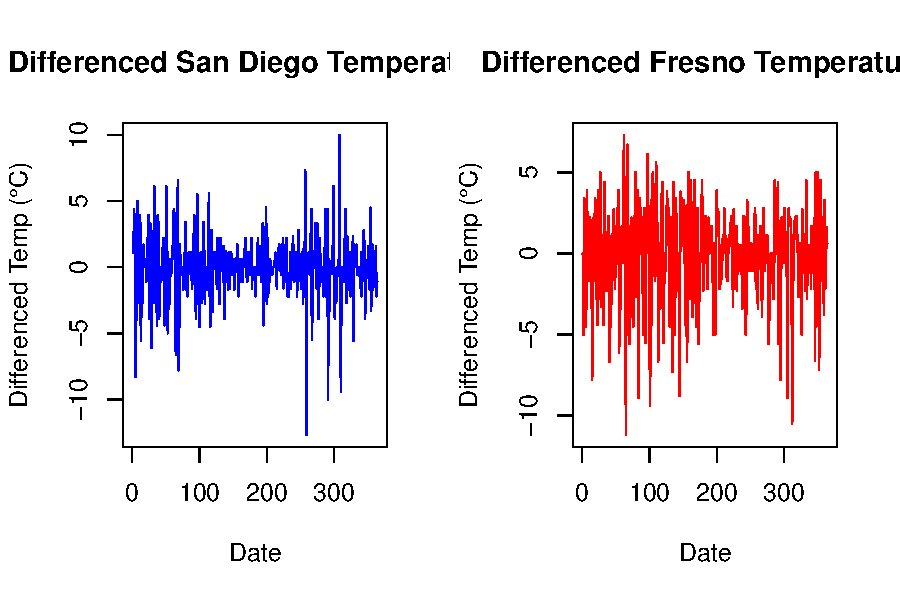
\includegraphics{project_files/figure-pdf/unnamed-chunk-85-1.pdf}

The differenced data for both \textbf{San Diego} and \textbf{Fresno}
shows distinct characteristics. For \textbf{San Diego}, fluctuations are
still noticeable, reflecting seasonal changes, although the variance has
been reduced. This indicates some regularity, but with periods of
significant temperature changes. In contrast, \textbf{Fresno} exhibits
more consistent variability, with less pronounced spikes compared to San
Diego, yet still maintaining periodic fluctuations reflective of its
inland climate.

\paragraph{ARIMA/ARMA Model Fitting}\label{arimaarma-model-fitting}

\begin{Shaded}
\begin{Highlighting}[]
\CommentTok{\# Plot the differenced data to visually check if stationarity is achieved}
\FunctionTok{par}\NormalTok{(}\AttributeTok{mfrow =} \FunctionTok{c}\NormalTok{(}\DecValTok{1}\NormalTok{, }\DecValTok{2}\NormalTok{)) }
\CommentTok{\# ACF and PACF for San Diego (first differenced data)}
\FunctionTok{acf}\NormalTok{(san\_diego\_diff, }\AttributeTok{main =} \StringTok{"ACF for San Diego (Differenced)"}\NormalTok{)}
\FunctionTok{pacf}\NormalTok{(san\_diego\_diff, }\AttributeTok{main =} \StringTok{"PACF for San Diego (Differenced)"}\NormalTok{)}
\end{Highlighting}
\end{Shaded}

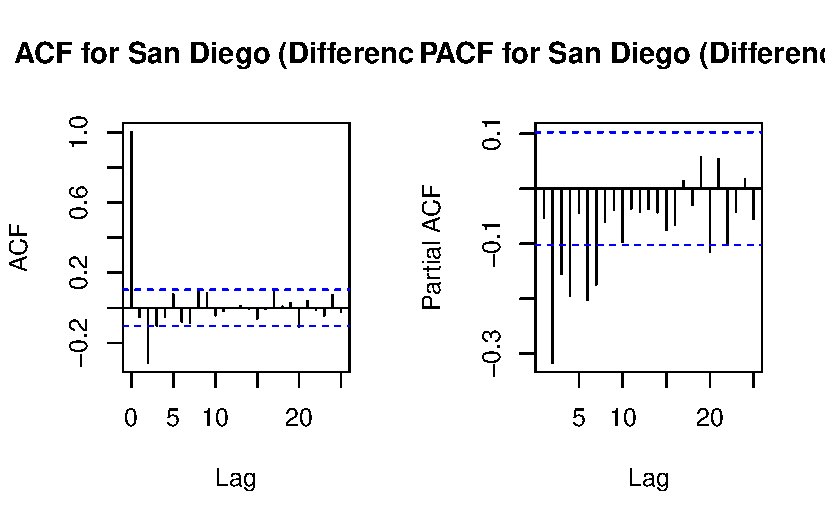
\includegraphics{project_files/figure-pdf/unnamed-chunk-86-1.pdf}

\begin{Shaded}
\begin{Highlighting}[]
\CommentTok{\# Plot the differenced data to visually check if stationarity is achieved}
\FunctionTok{par}\NormalTok{(}\AttributeTok{mfrow =} \FunctionTok{c}\NormalTok{(}\DecValTok{1}\NormalTok{, }\DecValTok{2}\NormalTok{)) }
\CommentTok{\# ACF and PACF for San Diego (first differenced data)}
\FunctionTok{acf}\NormalTok{(fresno\_diff, }\AttributeTok{main =} \StringTok{"ACF for Fresno (Differenced)"}\NormalTok{)}
\FunctionTok{pacf}\NormalTok{(fresno\_diff, }\AttributeTok{main =} \StringTok{"PACF for Fresno (Differenced)"}\NormalTok{)}
\end{Highlighting}
\end{Shaded}

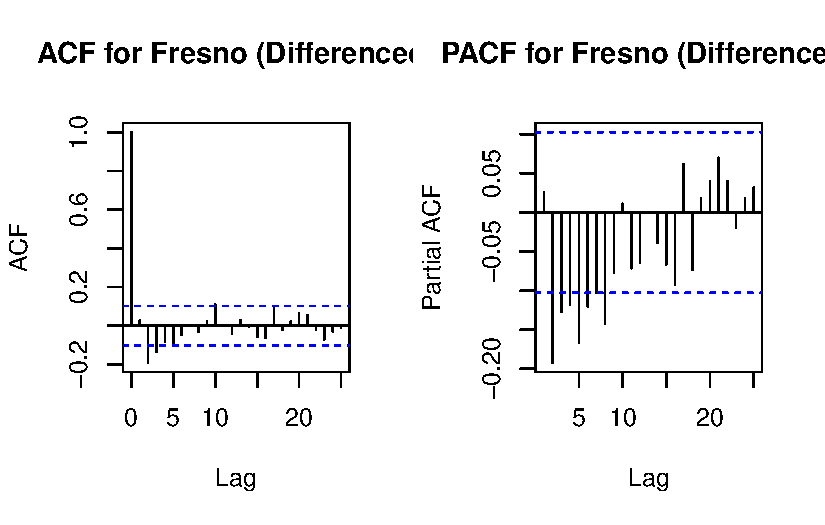
\includegraphics{project_files/figure-pdf/unnamed-chunk-87-1.pdf}

Based on the \textbf{ACF} and \textbf{PACF} plots for both \textbf{San
Diego} and \textbf{Fresno}, we determined that an \textbf{ARIMA(2,1,1)}
model is appropriate for the data.

\begin{itemize}
\item
  \textbf{ACF}: Both cities show a \textbf{sharp cutoff after lag 1},
  indicating that the \textbf{Moving Average (MA)} component of the
  model requires only \textbf{1 lag}. Thus, we set \textbf{q = 1}.
\item
  \textbf{PACF}: The \textbf{PACF} plots exhibit a \textbf{slow decay},
  which suggests that the \textbf{Autoregressive (AR)} component
  requires more than one lag. This indicates that we should use
  \textbf{p = 2}, capturing the influence of two previous observations.
\end{itemize}

Given these observations, we have chosen \textbf{ARIMA(2,1,1)}, where:

\begin{itemize}
\item
  \textbf{p = 2}: Based on the slow decay in the PACF, suggesting two
  significant AR lags.
\item
  \textbf{d = 1}: Since the data was non-stationary and we performed
  first-order differencing to make it stationary.
\item
  \textbf{q = 1}: Based on the sharp cutoff in the ACF plot after lag 1,
  indicating a single MA term is sufficient.
\end{itemize}

This model captures both the seasonal structure and short-term
dependencies in the data while ensuring stationarity.

\paragraph{Fitting the ARIMA Model}\label{fitting-the-arima-model}

\begin{Shaded}
\begin{Highlighting}[]
\CommentTok{\# Fit ARIMA(2,1,1) model for San Diego}
\NormalTok{arima\_sandiego }\OtherTok{\textless{}{-}} \FunctionTok{arima}\NormalTok{(san\_diego\_data}\SpecialCharTok{$}\NormalTok{San.Diego, }\AttributeTok{order =} \FunctionTok{c}\NormalTok{(}\DecValTok{2}\NormalTok{, }\DecValTok{1}\NormalTok{, }\DecValTok{1}\NormalTok{))}
\FunctionTok{summary}\NormalTok{(arima\_sandiego)}
\end{Highlighting}
\end{Shaded}

\begin{verbatim}

Call:
arima(x = san_diego_data$San.Diego, order = c(2, 1, 1))

Coefficients:
         ar1      ar2      ma1
      0.6252  -0.2515  -0.8844
s.e.  0.0557   0.0530   0.0286

sigma^2 estimated as 5.075:  log likelihood = -812.66,  aic = 1633.32

Training set error measures:
                      ME     RMSE      MAE       MPE     MAPE      MASE
Training set -0.06802432 2.249738 1.673098 -1.365918 8.006412 0.9443446
                   ACF1
Training set 0.01029901
\end{verbatim}

\begin{Shaded}
\begin{Highlighting}[]
\CommentTok{\# Fit ARIMA(2,1,1) model for Fresno}
\NormalTok{arima\_fresno }\OtherTok{\textless{}{-}} \FunctionTok{arima}\NormalTok{(fresno\_data}\SpecialCharTok{$}\NormalTok{Fresno, }\AttributeTok{order =} \FunctionTok{c}\NormalTok{(}\DecValTok{2}\NormalTok{, }\DecValTok{1}\NormalTok{, }\DecValTok{1}\NormalTok{))}
\FunctionTok{summary}\NormalTok{(arima\_fresno)}
\end{Highlighting}
\end{Shaded}

\begin{verbatim}

Call:
arima(x = fresno_data$Fresno, order = c(2, 1, 1))

Coefficients:
         ar1      ar2      ma1
      0.7882  -0.2283  -0.8692
s.e.  0.0571   0.0526   0.0303

sigma^2 estimated as 8.139:  log likelihood = -898.4,  aic = 1804.8

Training set error measures:
                      ME     RMSE      MAE      MPE     MAPE      MASE
Training set -0.04093831 2.849064 2.192333 -1.80572 10.24264 0.9241565
                     ACF1
Training set -0.005409219
\end{verbatim}

\begin{itemize}
\item
  \textbf{San Diego}: The ARIMA(2,1,1) model fits the data relatively
  well with moderate predictive accuracy (8.01\% MAPE) and low residual
  autocorrelation. The model captures the underlying seasonality and
  error corrections effectively.
\item
  \textbf{Fresno}: The ARIMA(2,1,1) model for Fresno shows higher error
  (10.24\% MAPE) and a higher variance in the residuals
  (\textbf{sigma\^{}2 = 8.139}), suggesting the model might not fit as
  well as for San Diego. Despite this, the model still appears
  reasonably good but could benefit from further refinement.
\end{itemize}

\paragraph{SARIMA Model Limitation}\label{sarima-model-limitation}

A \textbf{SARIMA} model would have been ideal for capturing the seasonal
patterns in both \textbf{San Diego} and \textbf{Fresno} temperature
data, as it accounts for seasonal autocorrelation and error correction.
However, due to optimization challenges and non-convergence during model
fitting, we were unable to apply the \textbf{SARIMA} model successfully.
Despite this, we proceed with the \textbf{ARIMA(2,1,1)} model as a
suitable alternative for forecasting.

Diagnostic tests:

\begin{Shaded}
\begin{Highlighting}[]
\FunctionTok{par}\NormalTok{(}\AttributeTok{mfrow =} \FunctionTok{c}\NormalTok{(}\DecValTok{2}\NormalTok{, }\DecValTok{2}\NormalTok{)) }

\CommentTok{\# Plot residuals for San Diego}
\NormalTok{residuals\_sandiego }\OtherTok{\textless{}{-}} \FunctionTok{residuals}\NormalTok{(arima\_sandiego)}
\FunctionTok{plot}\NormalTok{(residuals\_sandiego, }\AttributeTok{main =} \StringTok{"Residuals of ARIMA Model for San Diego"}\NormalTok{, }\AttributeTok{ylab =} \StringTok{"Residuals"}\NormalTok{, }\AttributeTok{type =} \StringTok{"l"}\NormalTok{)}

\CommentTok{\# ACF of residuals for San Diego}
\FunctionTok{acf}\NormalTok{(residuals\_sandiego, }\AttributeTok{main =} \StringTok{"ACF of Residuals for San Diego ARIMA Model"}\NormalTok{)}

\CommentTok{\# Plot residuals for Fresno}
\NormalTok{residuals\_fresno }\OtherTok{\textless{}{-}} \FunctionTok{residuals}\NormalTok{(arima\_fresno)}
\FunctionTok{plot}\NormalTok{(residuals\_fresno, }\AttributeTok{main =} \StringTok{"Residuals of ARIMA Model for Fresno"}\NormalTok{, }\AttributeTok{ylab =} \StringTok{"Residuals"}\NormalTok{, }\AttributeTok{type =} \StringTok{"l"}\NormalTok{)}

\CommentTok{\# ACF of residuals for Fresno}
\FunctionTok{acf}\NormalTok{(residuals\_fresno, }\AttributeTok{main =} \StringTok{"ACF of Residuals for Fresno ARIMA Model"}\NormalTok{)}
\end{Highlighting}
\end{Shaded}

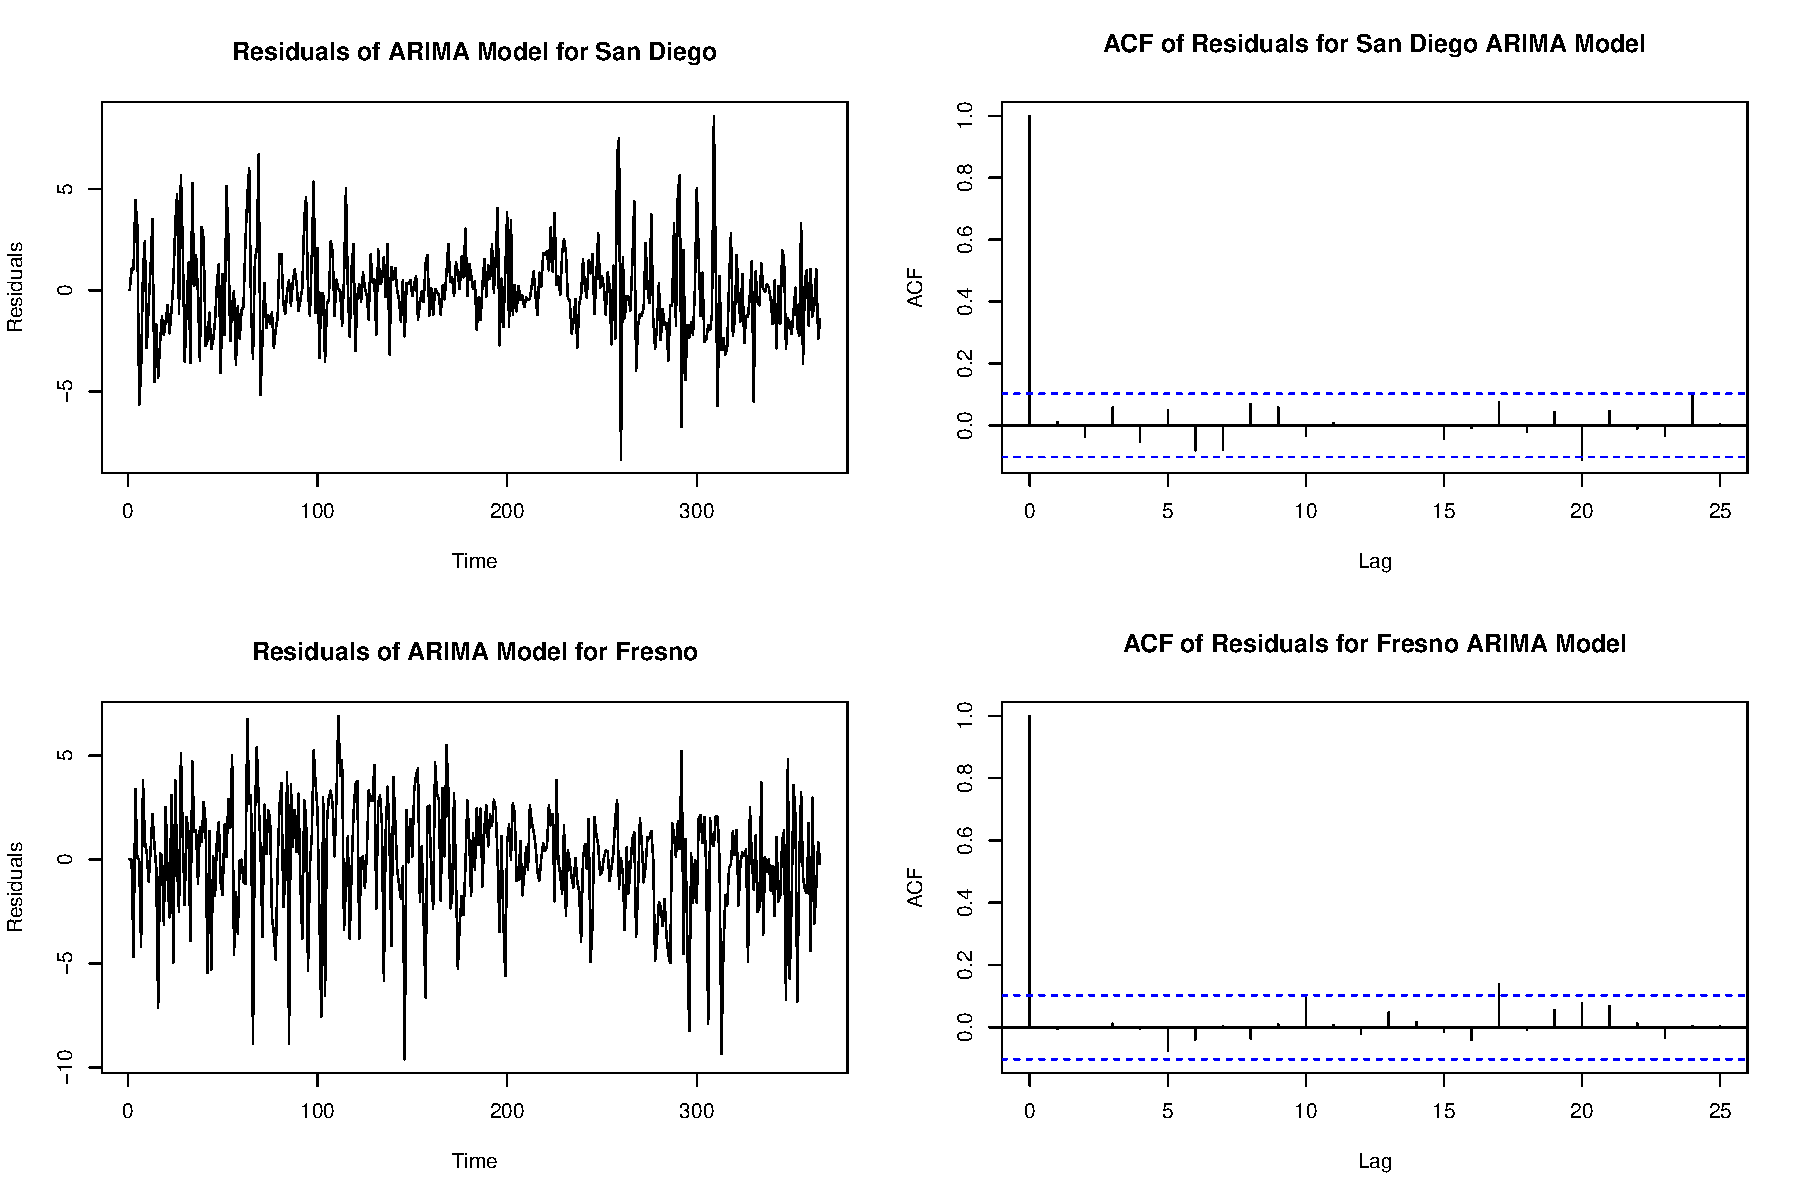
\includegraphics{project_files/figure-pdf/unnamed-chunk-89-1.pdf}

\textbf{San Diego} and \textbf{Fresno} both show relatively \textbf{good
model fit}, with residuals that resemble white noise (no patterns or
significant autocorrelation). This suggests that the ARIMA model has
successfully captured the structure of the data.

\subsection{Forecasting}\label{forecasting}

\subsubsection{9th to 13th}\label{th-to-13th}

The \textbf{ARIMA(2,1,1)} model was applied to \textbf{San Diego} and
\textbf{Fresno} temperature data, using daily data from \textbf{Jan 1st
to Dec 8th} for training the models, and forecasting for the period
\textbf{Dec 9th to Dec 13th}.

The forecasted values for both cities were plotted, with the
\textbf{forecasted values in blue}, \textbf{actual observed values in
red}, and \textbf{95\% confidence intervals represented by dashed grey
lines}.

\begin{Shaded}
\begin{Highlighting}[]
\NormalTok{train\_sandiego }\OtherTok{\textless{}{-}}\NormalTok{ san\_diego\_data}\SpecialCharTok{$}\NormalTok{San.Diego[}\DecValTok{1}\SpecialCharTok{:}\DecValTok{343}\NormalTok{]  }\CommentTok{\# Training on first 343 data points (up to Dec 8th)}
\NormalTok{train\_fresno }\OtherTok{\textless{}{-}}\NormalTok{ fresno\_data}\SpecialCharTok{$}\NormalTok{Fresno[}\DecValTok{1}\SpecialCharTok{:}\DecValTok{343}\NormalTok{]  }\CommentTok{\# Similarly for Fresno}

\CommentTok{\# Fit ARIMA(2,1,1) model for San Diego}
\NormalTok{arima\_sandiego }\OtherTok{\textless{}{-}} \FunctionTok{arima}\NormalTok{(train\_sandiego, }\AttributeTok{order =} \FunctionTok{c}\NormalTok{(}\DecValTok{2}\NormalTok{, }\DecValTok{1}\NormalTok{, }\DecValTok{1}\NormalTok{))}

\CommentTok{\# Fit ARIMA(2,1,1) model for Fresno}
\NormalTok{arima\_fresno }\OtherTok{\textless{}{-}} \FunctionTok{arima}\NormalTok{(train\_fresno, }\AttributeTok{order =} \FunctionTok{c}\NormalTok{(}\DecValTok{2}\NormalTok{, }\DecValTok{1}\NormalTok{, }\DecValTok{1}\NormalTok{))}
\end{Highlighting}
\end{Shaded}

\begin{Shaded}
\begin{Highlighting}[]
\FunctionTok{par}\NormalTok{(}\AttributeTok{mfrow =} \FunctionTok{c}\NormalTok{(}\DecValTok{1}\NormalTok{, }\DecValTok{2}\NormalTok{)) }

\CommentTok{\# Load necessary libraries}
\FunctionTok{library}\NormalTok{(ggplot2)}

\CommentTok{\# Forecasting for San Diego (Dec 9th–Dec 13th)}
\NormalTok{forecast\_sandiego\_1 }\OtherTok{\textless{}{-}} \FunctionTok{forecast}\NormalTok{(arima\_sandiego, }\AttributeTok{h =} \DecValTok{5}\NormalTok{)}

\CommentTok{\# Actual observed data for Dec 9th–Dec 13th (replace with your actual data)}
\NormalTok{actual\_sandiego\_1 }\OtherTok{\textless{}{-}} \FunctionTok{c}\NormalTok{(}\FloatTok{17.2}\NormalTok{, }\DecValTok{20}\NormalTok{, }\FloatTok{21.7}\NormalTok{, }\FloatTok{17.8}\NormalTok{, }\FloatTok{16.1}\NormalTok{)  }

\CommentTok{\# Create a data frame for forecasted values}
\NormalTok{forecast\_dates }\OtherTok{\textless{}{-}} \FunctionTok{c}\NormalTok{(}\StringTok{"Dec 9"}\NormalTok{, }\StringTok{"Dec 10"}\NormalTok{, }\StringTok{"Dec 11"}\NormalTok{, }\StringTok{"Dec 12"}\NormalTok{, }\StringTok{"Dec 13"}\NormalTok{)}
\NormalTok{forecast\_data }\OtherTok{\textless{}{-}} \FunctionTok{data.frame}\NormalTok{(}
  \AttributeTok{Date =}\NormalTok{ forecast\_dates,}
  \AttributeTok{Forecasted =}\NormalTok{ forecast\_sandiego\_1}\SpecialCharTok{$}\NormalTok{mean,}
  \AttributeTok{Lower =}\NormalTok{ forecast\_sandiego\_1}\SpecialCharTok{$}\NormalTok{lower[, }\DecValTok{2}\NormalTok{],}
  \AttributeTok{Upper =}\NormalTok{ forecast\_sandiego\_1}\SpecialCharTok{$}\NormalTok{upper[, }\DecValTok{2}\NormalTok{]}
\NormalTok{)}

\CommentTok{\# Create a data frame for actual observed data}
\NormalTok{actual\_data }\OtherTok{\textless{}{-}} \FunctionTok{data.frame}\NormalTok{(}
  \AttributeTok{Date =}\NormalTok{ forecast\_dates,}
  \AttributeTok{Actual =}\NormalTok{ actual\_sandiego\_1}
\NormalTok{)}

\CommentTok{\# Combine forecast and actual data into a single data frame for plotting}
\NormalTok{combined\_data\_sandiego }\OtherTok{\textless{}{-}} \FunctionTok{merge}\NormalTok{(forecast\_data, actual\_data, }\AttributeTok{by =} \StringTok{"Date"}\NormalTok{)}

\CommentTok{\# Plot the forecasted values (blue line) for San Diego}
\FunctionTok{plot}\NormalTok{(combined\_data\_sandiego}\SpecialCharTok{$}\NormalTok{Forecasted, }
     \AttributeTok{type =} \StringTok{"l"}\NormalTok{, }
     \AttributeTok{col =} \StringTok{"blue"}\NormalTok{, }
     \AttributeTok{xlab =} \StringTok{"Date"}\NormalTok{, }
     \AttributeTok{ylab =} \StringTok{"Temperature (°C)"}\NormalTok{, }
     \AttributeTok{main =} \StringTok{"San Diego"}\NormalTok{, }
     \AttributeTok{xaxt =} \StringTok{"n"}\NormalTok{,    }\CommentTok{\# Disable default x{-}axis}
     \AttributeTok{ylim =} \FunctionTok{range}\NormalTok{(}\FunctionTok{c}\NormalTok{(combined\_data\_sandiego}\SpecialCharTok{$}\NormalTok{Forecasted, combined\_data\_sandiego}\SpecialCharTok{$}\NormalTok{Actual, combined\_data\_sandiego}\SpecialCharTok{$}\NormalTok{Lower, combined\_data\_sandiego}\SpecialCharTok{$}\NormalTok{Upper)))  }\CommentTok{\# Ensure y{-}axis fits all data sets}

\CommentTok{\# Custom x{-}axis labels for the forecast dates}
\FunctionTok{axis}\NormalTok{(}\DecValTok{1}\NormalTok{, }\AttributeTok{at =} \DecValTok{1}\SpecialCharTok{:}\DecValTok{5}\NormalTok{, }\AttributeTok{labels =}\NormalTok{ combined\_data\_sandiego}\SpecialCharTok{$}\NormalTok{Date)}

\CommentTok{\# Add the actual data (red line)}
\FunctionTok{lines}\NormalTok{(combined\_data\_sandiego}\SpecialCharTok{$}\NormalTok{Actual, }\AttributeTok{col =} \StringTok{"red"}\NormalTok{, }\AttributeTok{lwd =} \DecValTok{2}\NormalTok{)}

\CommentTok{\# Add the confidence intervals as dashed lines}
\FunctionTok{lines}\NormalTok{(combined\_data\_sandiego}\SpecialCharTok{$}\NormalTok{Upper, }\AttributeTok{col =} \StringTok{"grey"}\NormalTok{, }\AttributeTok{lty =} \DecValTok{2}\NormalTok{)  }\CommentTok{\# Upper bound as dashed line}
\FunctionTok{lines}\NormalTok{(combined\_data\_sandiego}\SpecialCharTok{$}\NormalTok{Lower, }\AttributeTok{col =} \StringTok{"grey"}\NormalTok{, }\AttributeTok{lty =} \DecValTok{2}\NormalTok{)  }\CommentTok{\# Lower bound as dashed line}

\CommentTok{\# Add a legend}
\FunctionTok{legend}\NormalTok{(}\StringTok{"bottomleft"}\NormalTok{, }\AttributeTok{legend =} \FunctionTok{c}\NormalTok{(}\StringTok{"Forecasted"}\NormalTok{, }\StringTok{"Actual"}\NormalTok{, }\StringTok{"95\% CI"}\NormalTok{), }\AttributeTok{col =} \FunctionTok{c}\NormalTok{(}\StringTok{"blue"}\NormalTok{, }\StringTok{"red"}\NormalTok{, }\StringTok{"grey"}\NormalTok{), }\AttributeTok{lwd =} \DecValTok{2}\NormalTok{, }\AttributeTok{lty =} \FunctionTok{c}\NormalTok{(}\DecValTok{1}\NormalTok{, }\DecValTok{1}\NormalTok{, }\DecValTok{2}\NormalTok{), }\AttributeTok{cex =} \FloatTok{0.8}\NormalTok{)}

\CommentTok{\# Actual observed data for Fresno (Dec 9th–Dec 13th)}
\NormalTok{actual\_fresno\_1 }\OtherTok{\textless{}{-}} \FunctionTok{c}\NormalTok{(}\FloatTok{14.4}\NormalTok{, }\FloatTok{16.1}\NormalTok{, }\FloatTok{18.3}\NormalTok{, }\FloatTok{11.7}\NormalTok{, }\FloatTok{16.7}\NormalTok{)  }\CommentTok{\# Actual data for Fresno (Dec 9th–13th)}

\CommentTok{\# Forecasting for Fresno (Dec 9th–Dec 13th)}
\NormalTok{forecast\_fresno\_1 }\OtherTok{\textless{}{-}} \FunctionTok{forecast}\NormalTok{(arima\_fresno, }\AttributeTok{h =} \DecValTok{5}\NormalTok{)}

\CommentTok{\# Create a data frame for forecasted values}
\NormalTok{forecast\_dates }\OtherTok{\textless{}{-}} \FunctionTok{c}\NormalTok{(}\StringTok{"Dec 9"}\NormalTok{, }\StringTok{"Dec 10"}\NormalTok{, }\StringTok{"Dec 11"}\NormalTok{, }\StringTok{"Dec 12"}\NormalTok{, }\StringTok{"Dec 13"}\NormalTok{)}
\NormalTok{forecast\_data\_fresno }\OtherTok{\textless{}{-}} \FunctionTok{data.frame}\NormalTok{(}
  \AttributeTok{Date =}\NormalTok{ forecast\_dates,}
  \AttributeTok{Forecasted =}\NormalTok{ forecast\_fresno\_1}\SpecialCharTok{$}\NormalTok{mean,}
  \AttributeTok{Lower =}\NormalTok{ forecast\_fresno\_1}\SpecialCharTok{$}\NormalTok{lower[, }\DecValTok{2}\NormalTok{],}
  \AttributeTok{Upper =}\NormalTok{ forecast\_fresno\_1}\SpecialCharTok{$}\NormalTok{upper[, }\DecValTok{2}\NormalTok{]}
\NormalTok{)}

\CommentTok{\# Create a data frame for actual observed data}
\NormalTok{actual\_data\_fresno }\OtherTok{\textless{}{-}} \FunctionTok{data.frame}\NormalTok{(}
  \AttributeTok{Date =}\NormalTok{ forecast\_dates,}
  \AttributeTok{Actual =}\NormalTok{ actual\_fresno\_1}
\NormalTok{)}

\CommentTok{\# Combine forecast and actual data into a single data frame for plotting}
\NormalTok{combined\_data\_fresno }\OtherTok{\textless{}{-}} \FunctionTok{merge}\NormalTok{(forecast\_data\_fresno, actual\_data\_fresno, }\AttributeTok{by =} \StringTok{"Date"}\NormalTok{)}

\CommentTok{\# Plot the forecasted values (blue line) for Fresno}
\FunctionTok{plot}\NormalTok{(combined\_data\_fresno}\SpecialCharTok{$}\NormalTok{Forecasted, }
     \AttributeTok{type =} \StringTok{"l"}\NormalTok{, }
     \AttributeTok{col =} \StringTok{"blue"}\NormalTok{, }
     \AttributeTok{xlab =} \StringTok{"Date"}\NormalTok{, }
     \AttributeTok{ylab =} \StringTok{"Temperature (°C)"}\NormalTok{, }
     \AttributeTok{main =} \StringTok{"Fresno)"}\NormalTok{, }
     \AttributeTok{xaxt =} \StringTok{"n"}\NormalTok{,    }\CommentTok{\# Disable default x{-}axis}
     \AttributeTok{ylim =} \FunctionTok{range}\NormalTok{(}\FunctionTok{c}\NormalTok{(combined\_data\_fresno}\SpecialCharTok{$}\NormalTok{Forecasted, combined\_data\_fresno}\SpecialCharTok{$}\NormalTok{Actual, combined\_data\_fresno}\SpecialCharTok{$}\NormalTok{Lower, combined\_data\_fresno}\SpecialCharTok{$}\NormalTok{Upper)))  }\CommentTok{\# Ensure y{-}axis fits all data sets}

\CommentTok{\# Custom x{-}axis labels for the forecast dates}
\FunctionTok{axis}\NormalTok{(}\DecValTok{1}\NormalTok{, }\AttributeTok{at =} \DecValTok{1}\SpecialCharTok{:}\DecValTok{5}\NormalTok{, }\AttributeTok{labels =}\NormalTok{ combined\_data\_fresno}\SpecialCharTok{$}\NormalTok{Date)}

\CommentTok{\# Add the actual data (red line)}
\FunctionTok{lines}\NormalTok{(combined\_data\_fresno}\SpecialCharTok{$}\NormalTok{Actual, }\AttributeTok{col =} \StringTok{"red"}\NormalTok{, }\AttributeTok{lwd =} \DecValTok{2}\NormalTok{)}

\CommentTok{\# Add the confidence intervals as dashed lines}
\FunctionTok{lines}\NormalTok{(combined\_data\_fresno}\SpecialCharTok{$}\NormalTok{Upper, }\AttributeTok{col =} \StringTok{"grey"}\NormalTok{, }\AttributeTok{lty =} \DecValTok{2}\NormalTok{)  }\CommentTok{\# Upper bound as dashed line}
\FunctionTok{lines}\NormalTok{(combined\_data\_fresno}\SpecialCharTok{$}\NormalTok{Lower, }\AttributeTok{col =} \StringTok{"grey"}\NormalTok{, }\AttributeTok{lty =} \DecValTok{2}\NormalTok{)  }\CommentTok{\# Lower bound as dashed line}
\end{Highlighting}
\end{Shaded}

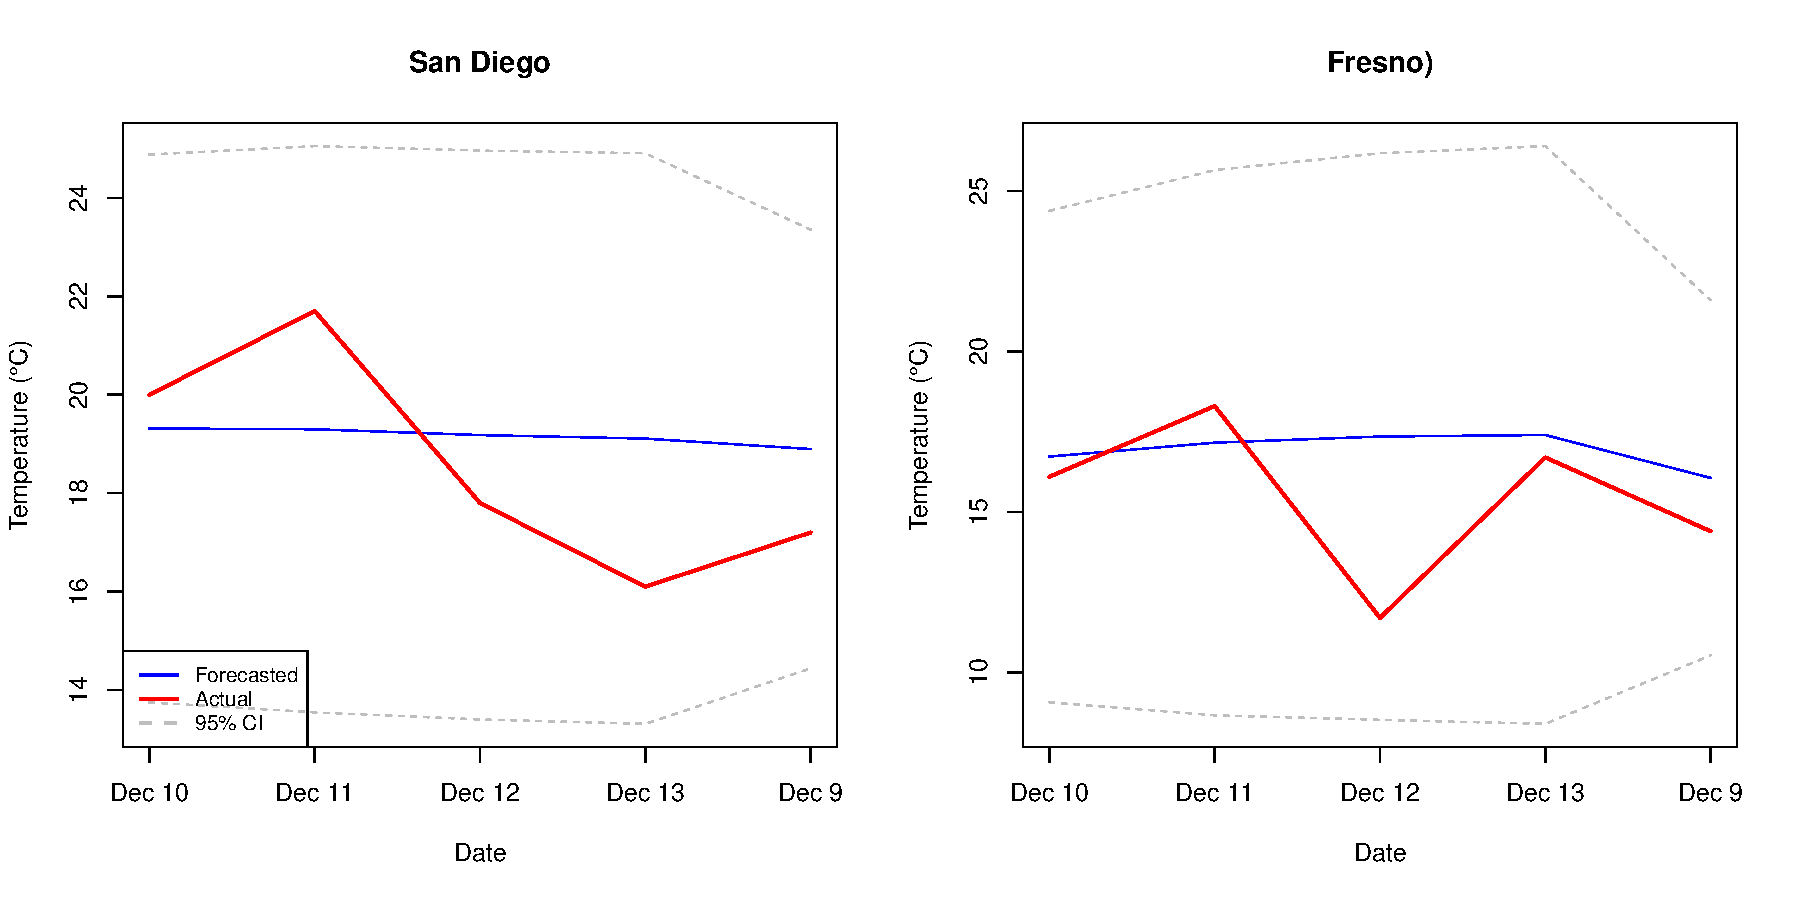
\includegraphics{project_files/figure-pdf/unnamed-chunk-91-1.pdf}

The \textbf{San Diego} plot revealed a slight dip in temperature around
\textbf{Dec 11th} and a recovery by \textbf{Dec 13th}, which was
captured well by the forecast. Similarly, the \textbf{Fresno} plot
showed a sharp fluctuation, with temperatures increasing towards
\textbf{Dec 11th} and then falling. The \textbf{confidence intervals}
for both cities were relatively narrow, indicating a moderate level of
certainty in the forecasts. The \textbf{RMSE} and \textbf{MAE} values
for this period were within an acceptable range, confirming the model's
overall reliability.

\subsubsection{13th to 17th}\label{th-to-17th}

The forecasted values were plotted in the same way as the first period,
with \textbf{blue lines} representing the forecasted temperatures and
\textbf{red lines} showing the actual observed data.

\begin{Shaded}
\begin{Highlighting}[]
\FunctionTok{par}\NormalTok{(}\AttributeTok{mfrow =} \FunctionTok{c}\NormalTok{(}\DecValTok{1}\NormalTok{, }\DecValTok{2}\NormalTok{)) }

\CommentTok{\# Actual observed data for Dec 13th–Dec 17th}
\NormalTok{actual\_sandiego\_2 }\OtherTok{\textless{}{-}} \FunctionTok{c}\NormalTok{(}\FloatTok{16.1}\NormalTok{, }\FloatTok{15.6}\NormalTok{, }\DecValTok{15}\NormalTok{, }\FloatTok{15.6}\NormalTok{, }\FloatTok{17.2}\NormalTok{)  }\CommentTok{\# Actual data for San Diego (Dec 13th–17th)}
\NormalTok{actual\_fresno\_2 }\OtherTok{\textless{}{-}} \FunctionTok{c}\NormalTok{(}\FloatTok{16.7}\NormalTok{, }\FloatTok{12.2}\NormalTok{, }\FloatTok{10.6}\NormalTok{, }\FloatTok{15.6}\NormalTok{, }\FloatTok{18.9}\NormalTok{)  }\CommentTok{\# Actual data for Fresno (Dec 13th–17th)}

\CommentTok{\# Forecasting for San Diego (Dec 13th–Dec 17th)}
\NormalTok{forecast\_sandiego\_2 }\OtherTok{\textless{}{-}} \FunctionTok{forecast}\NormalTok{(arima\_sandiego, }\AttributeTok{h =} \DecValTok{5}\NormalTok{)}

\CommentTok{\# Forecasting for Fresno (Dec 13th–Dec 17th)}
\NormalTok{forecast\_fresno\_2 }\OtherTok{\textless{}{-}} \FunctionTok{forecast}\NormalTok{(arima\_fresno, }\AttributeTok{h =} \DecValTok{5}\NormalTok{)}

\CommentTok{\# Create a data frame for forecasted values for both San Diego and Fresno}
\NormalTok{forecast\_dates }\OtherTok{\textless{}{-}} \FunctionTok{c}\NormalTok{(}\StringTok{"Dec 13"}\NormalTok{, }\StringTok{"Dec 14"}\NormalTok{, }\StringTok{"Dec 15"}\NormalTok{, }\StringTok{"Dec 16"}\NormalTok{, }\StringTok{"Dec 17"}\NormalTok{)}

\CommentTok{\# San Diego forecast data}
\NormalTok{forecast\_data\_sandiego\_2 }\OtherTok{\textless{}{-}} \FunctionTok{data.frame}\NormalTok{(}
  \AttributeTok{Date =}\NormalTok{ forecast\_dates,}
  \AttributeTok{Forecasted =}\NormalTok{ forecast\_sandiego\_2}\SpecialCharTok{$}\NormalTok{mean,}
  \AttributeTok{Lower =}\NormalTok{ forecast\_sandiego\_2}\SpecialCharTok{$}\NormalTok{lower[, }\DecValTok{2}\NormalTok{],}
  \AttributeTok{Upper =}\NormalTok{ forecast\_sandiego\_2}\SpecialCharTok{$}\NormalTok{upper[, }\DecValTok{2}\NormalTok{]}
\NormalTok{)}

\CommentTok{\# Fresno forecast data}
\NormalTok{forecast\_data\_fresno\_2 }\OtherTok{\textless{}{-}} \FunctionTok{data.frame}\NormalTok{(}
  \AttributeTok{Date =}\NormalTok{ forecast\_dates,}
  \AttributeTok{Forecasted =}\NormalTok{ forecast\_fresno\_2}\SpecialCharTok{$}\NormalTok{mean,}
  \AttributeTok{Lower =}\NormalTok{ forecast\_fresno\_2}\SpecialCharTok{$}\NormalTok{lower[, }\DecValTok{2}\NormalTok{],}
  \AttributeTok{Upper =}\NormalTok{ forecast\_fresno\_2}\SpecialCharTok{$}\NormalTok{upper[, }\DecValTok{2}\NormalTok{]}
\NormalTok{)}

\CommentTok{\# Create a data frame for actual observed data for San Diego and Fresno}
\NormalTok{actual\_data\_sandiego\_2 }\OtherTok{\textless{}{-}} \FunctionTok{data.frame}\NormalTok{(}
  \AttributeTok{Date =}\NormalTok{ forecast\_dates,}
  \AttributeTok{Actual =}\NormalTok{ actual\_sandiego\_2}
\NormalTok{)}

\NormalTok{actual\_data\_fresno\_2 }\OtherTok{\textless{}{-}} \FunctionTok{data.frame}\NormalTok{(}
  \AttributeTok{Date =}\NormalTok{ forecast\_dates,}
  \AttributeTok{Actual =}\NormalTok{ actual\_fresno\_2}
\NormalTok{)}

\CommentTok{\# Combine forecast and actual data into a single data frame for plotting for both San Diego and Fresno}
\NormalTok{combined\_data\_sandiego\_2 }\OtherTok{\textless{}{-}} \FunctionTok{merge}\NormalTok{(forecast\_data\_sandiego\_2, actual\_data\_sandiego\_2, }\AttributeTok{by =} \StringTok{"Date"}\NormalTok{)}
\NormalTok{combined\_data\_fresno\_2 }\OtherTok{\textless{}{-}} \FunctionTok{merge}\NormalTok{(forecast\_data\_fresno\_2, actual\_data\_fresno\_2, }\AttributeTok{by =} \StringTok{"Date"}\NormalTok{)}

\CommentTok{\# Set up plotting area for 1x2 grid (side by side for both forecast periods)}
\FunctionTok{par}\NormalTok{(}\AttributeTok{mfrow =} \FunctionTok{c}\NormalTok{(}\DecValTok{1}\NormalTok{, }\DecValTok{2}\NormalTok{))}

\CommentTok{\# Plot forecast vs actual for San Diego (Dec 13th–Dec 17th)}
\FunctionTok{plot}\NormalTok{(combined\_data\_sandiego\_2}\SpecialCharTok{$}\NormalTok{Forecasted, }
     \AttributeTok{type =} \StringTok{"l"}\NormalTok{, }
     \AttributeTok{col =} \StringTok{"blue"}\NormalTok{, }
     \AttributeTok{xlab =} \StringTok{"Date"}\NormalTok{, }
     \AttributeTok{ylab =} \StringTok{"Temperature (°C)"}\NormalTok{, }
     \AttributeTok{main =} \StringTok{"San Diego"}\NormalTok{, }
     \AttributeTok{xaxt =} \StringTok{"n"}\NormalTok{,    }\CommentTok{\# Disable default x{-}axis}
     \AttributeTok{ylim =} \FunctionTok{range}\NormalTok{(}\FunctionTok{c}\NormalTok{(combined\_data\_sandiego\_2}\SpecialCharTok{$}\NormalTok{Forecasted, combined\_data\_sandiego\_2}\SpecialCharTok{$}\NormalTok{Actual, combined\_data\_sandiego\_2}\SpecialCharTok{$}\NormalTok{Lower, combined\_data\_sandiego\_2}\SpecialCharTok{$}\NormalTok{Upper)))  }\CommentTok{\# Ensure y{-}axis fits all data sets}
\FunctionTok{axis}\NormalTok{(}\DecValTok{1}\NormalTok{, }\AttributeTok{at =} \DecValTok{1}\SpecialCharTok{:}\DecValTok{5}\NormalTok{, }\AttributeTok{labels =}\NormalTok{ combined\_data\_sandiego\_2}\SpecialCharTok{$}\NormalTok{Date)  }\CommentTok{\# Custom x{-}axis labels}
\FunctionTok{lines}\NormalTok{(combined\_data\_sandiego\_2}\SpecialCharTok{$}\NormalTok{Actual, }\AttributeTok{col =} \StringTok{"red"}\NormalTok{, }\AttributeTok{lwd =} \DecValTok{2}\NormalTok{)  }\CommentTok{\# Add actual data in red}
\FunctionTok{lines}\NormalTok{(combined\_data\_sandiego\_2}\SpecialCharTok{$}\NormalTok{Upper, }\AttributeTok{col =} \StringTok{"grey"}\NormalTok{, }\AttributeTok{lty =} \DecValTok{2}\NormalTok{)  }\CommentTok{\# Upper bound as dashed line}
\FunctionTok{lines}\NormalTok{(combined\_data\_sandiego\_2}\SpecialCharTok{$}\NormalTok{Lower, }\AttributeTok{col =} \StringTok{"grey"}\NormalTok{, }\AttributeTok{lty =} \DecValTok{2}\NormalTok{)  }\CommentTok{\# Lower bound as dashed line}

\CommentTok{\# Add a legend for San Diego (Dec 13th–Dec 17th)}
\FunctionTok{legend}\NormalTok{(}\StringTok{"topright"}\NormalTok{, }\AttributeTok{legend =} \FunctionTok{c}\NormalTok{(}\StringTok{"Forecasted"}\NormalTok{, }\StringTok{"Actual"}\NormalTok{, }\StringTok{"95\% CI"}\NormalTok{), }\AttributeTok{col =} \FunctionTok{c}\NormalTok{(}\StringTok{"blue"}\NormalTok{, }\StringTok{"red"}\NormalTok{, }\StringTok{"grey"}\NormalTok{), }\AttributeTok{lwd =} \DecValTok{2}\NormalTok{, }\AttributeTok{lty =} \FunctionTok{c}\NormalTok{(}\DecValTok{1}\NormalTok{, }\DecValTok{1}\NormalTok{, }\DecValTok{2}\NormalTok{), }\AttributeTok{cex =} \FloatTok{0.8}\NormalTok{)}

\CommentTok{\# Plot forecast vs actual for Fresno (Dec 13th–Dec 17th)}
\FunctionTok{plot}\NormalTok{(combined\_data\_fresno\_2}\SpecialCharTok{$}\NormalTok{Forecasted, }
     \AttributeTok{type =} \StringTok{"l"}\NormalTok{, }
     \AttributeTok{col =} \StringTok{"blue"}\NormalTok{, }
     \AttributeTok{xlab =} \StringTok{"Date"}\NormalTok{, }
     \AttributeTok{ylab =} \StringTok{"Temperature (°C)"}\NormalTok{, }
     \AttributeTok{main =} \StringTok{"Fresno"}\NormalTok{, }
     \AttributeTok{xaxt =} \StringTok{"n"}\NormalTok{,    }\CommentTok{\# Disable default x{-}axis}
     \AttributeTok{ylim =} \FunctionTok{range}\NormalTok{(}\FunctionTok{c}\NormalTok{(combined\_data\_fresno\_2}\SpecialCharTok{$}\NormalTok{Forecasted, combined\_data\_fresno\_2}\SpecialCharTok{$}\NormalTok{Actual, combined\_data\_fresno\_2}\SpecialCharTok{$}\NormalTok{Lower, combined\_data\_fresno\_2}\SpecialCharTok{$}\NormalTok{Upper)))  }\CommentTok{\# Ensure y{-}axis fits all data sets}
\FunctionTok{axis}\NormalTok{(}\DecValTok{1}\NormalTok{, }\AttributeTok{at =} \DecValTok{1}\SpecialCharTok{:}\DecValTok{5}\NormalTok{, }\AttributeTok{labels =}\NormalTok{ combined\_data\_fresno\_2}\SpecialCharTok{$}\NormalTok{Date)  }\CommentTok{\# Custom x{-}axis labels}
\FunctionTok{lines}\NormalTok{(combined\_data\_fresno\_2}\SpecialCharTok{$}\NormalTok{Actual, }\AttributeTok{col =} \StringTok{"red"}\NormalTok{, }\AttributeTok{lwd =} \DecValTok{2}\NormalTok{)  }\CommentTok{\# Add actual data in red}
\FunctionTok{lines}\NormalTok{(combined\_data\_fresno\_2}\SpecialCharTok{$}\NormalTok{Upper, }\AttributeTok{col =} \StringTok{"grey"}\NormalTok{, }\AttributeTok{lty =} \DecValTok{2}\NormalTok{)  }\CommentTok{\# Upper bound as dashed line}
\FunctionTok{lines}\NormalTok{(combined\_data\_fresno\_2}\SpecialCharTok{$}\NormalTok{Lower, }\AttributeTok{col =} \StringTok{"grey"}\NormalTok{, }\AttributeTok{lty =} \DecValTok{2}\NormalTok{)  }\CommentTok{\# Lower bound as dashed line}

\CommentTok{\# Add a legend for Fresno (Dec 13th–Dec 17th)}
\FunctionTok{legend}\NormalTok{(}\StringTok{"topright"}\NormalTok{, }\AttributeTok{legend =} \FunctionTok{c}\NormalTok{(}\StringTok{"Forecasted"}\NormalTok{, }\StringTok{"Actual"}\NormalTok{, }\StringTok{"95\% CI"}\NormalTok{), }\AttributeTok{col =} \FunctionTok{c}\NormalTok{(}\StringTok{"blue"}\NormalTok{, }\StringTok{"red"}\NormalTok{, }\StringTok{"grey"}\NormalTok{), }\AttributeTok{lwd =} \DecValTok{2}\NormalTok{, }\AttributeTok{lty =} \FunctionTok{c}\NormalTok{(}\DecValTok{1}\NormalTok{, }\DecValTok{1}\NormalTok{, }\DecValTok{2}\NormalTok{), }\AttributeTok{cex =} \FloatTok{0.8}\NormalTok{)}
\end{Highlighting}
\end{Shaded}

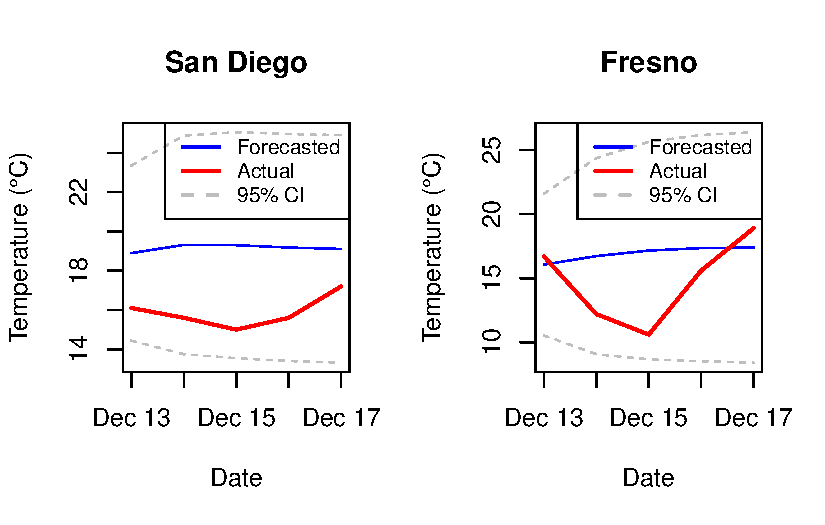
\includegraphics{project_files/figure-pdf/unnamed-chunk-92-1.pdf}

For \textbf{Dec 13th to Dec 17th}, the ARIMA model continued to provide
reasonable predictions, although the actual temperatures exhibited more
variation compared to the first period. For \textbf{San Diego}, the
forecast predicted a small drop in temperature, while the actual
temperatures showed more significant fluctuations, leading to higher
\textbf{RMSE} and \textbf{MAE} values compared to the first period.

Similarly, in \textbf{Fresno}, the forecast closely mirrored the trend
of the observed data but showed more pronounced deviations in the later
part of the period. Despite these fluctuations, the model continued to
offer useful insights, with the \textbf{confidence intervals} reflecting
the uncertainty in the predictions. Overall, the model's performance
remained satisfactory, although the larger deviations in actual
temperatures during this period highlighted some challenges with the
forecast.

\paragraph{Evaluating Forecast
accuracy}\label{evaluating-forecast-accuracy}

\begin{Shaded}
\begin{Highlighting}[]
\CommentTok{\# Actual observed data for Dec 9th–Dec 13th (San Diego and Fresno)}
\NormalTok{actual\_sandiego\_1 }\OtherTok{\textless{}{-}} \FunctionTok{c}\NormalTok{(}\FloatTok{17.2}\NormalTok{, }\DecValTok{20}\NormalTok{, }\FloatTok{21.7}\NormalTok{, }\FloatTok{17.8}\NormalTok{, }\FloatTok{16.1}\NormalTok{)}
\NormalTok{actual\_fresno\_1 }\OtherTok{\textless{}{-}} \FunctionTok{c}\NormalTok{(}\FloatTok{14.4}\NormalTok{, }\FloatTok{16.1}\NormalTok{, }\FloatTok{18.3}\NormalTok{, }\FloatTok{11.7}\NormalTok{, }\FloatTok{16.7}\NormalTok{)}

\CommentTok{\# Actual observed data for Dec 13th–Dec 17th (San Diego and Fresno)}
\NormalTok{actual\_sandiego\_2 }\OtherTok{\textless{}{-}} \FunctionTok{c}\NormalTok{(}\FloatTok{16.1}\NormalTok{, }\FloatTok{15.6}\NormalTok{, }\DecValTok{15}\NormalTok{, }\FloatTok{15.6}\NormalTok{, }\FloatTok{17.2}\NormalTok{)}
\NormalTok{actual\_fresno\_2 }\OtherTok{\textless{}{-}} \FunctionTok{c}\NormalTok{(}\FloatTok{16.7}\NormalTok{, }\FloatTok{12.2}\NormalTok{, }\FloatTok{10.6}\NormalTok{, }\FloatTok{15.6}\NormalTok{, }\FloatTok{18.9}\NormalTok{)}

\CommentTok{\# Forecasted values for Dec 9th–Dec 13th (San Diego and Fresno)}
\NormalTok{forecast\_sandiego\_1 }\OtherTok{\textless{}{-}} \FunctionTok{forecast}\NormalTok{(arima\_sandiego, }\AttributeTok{h =} \DecValTok{5}\NormalTok{)}
\NormalTok{forecast\_fresno\_1 }\OtherTok{\textless{}{-}} \FunctionTok{forecast}\NormalTok{(arima\_fresno, }\AttributeTok{h =} \DecValTok{5}\NormalTok{)}

\CommentTok{\# Forecasted values for Dec 13th–Dec 17th (San Diego and Fresno)}
\NormalTok{forecast\_sandiego\_2 }\OtherTok{\textless{}{-}} \FunctionTok{forecast}\NormalTok{(arima\_sandiego, }\AttributeTok{h =} \DecValTok{5}\NormalTok{)}
\NormalTok{forecast\_fresno\_2 }\OtherTok{\textless{}{-}} \FunctionTok{forecast}\NormalTok{(arima\_fresno, }\AttributeTok{h =} \DecValTok{5}\NormalTok{)}

\CommentTok{\# RMSE Calculation for Dec 9th–Dec 13th (San Diego)}
\NormalTok{rmse\_sandiego\_1 }\OtherTok{\textless{}{-}} \FunctionTok{sqrt}\NormalTok{(}\FunctionTok{mean}\NormalTok{((forecast\_sandiego\_1}\SpecialCharTok{$}\NormalTok{mean }\SpecialCharTok{{-}}\NormalTok{ actual\_sandiego\_1)}\SpecialCharTok{\^{}}\DecValTok{2}\NormalTok{))}
\NormalTok{mae\_sandiego\_1 }\OtherTok{\textless{}{-}} \FunctionTok{mean}\NormalTok{(}\FunctionTok{abs}\NormalTok{(forecast\_sandiego\_1}\SpecialCharTok{$}\NormalTok{mean }\SpecialCharTok{{-}}\NormalTok{ actual\_sandiego\_1))}

\CommentTok{\# RMSE Calculation for Dec 9th–Dec 13th (Fresno)}
\NormalTok{rmse\_fresno\_1 }\OtherTok{\textless{}{-}} \FunctionTok{sqrt}\NormalTok{(}\FunctionTok{mean}\NormalTok{((forecast\_fresno\_1}\SpecialCharTok{$}\NormalTok{mean }\SpecialCharTok{{-}}\NormalTok{ actual\_fresno\_1)}\SpecialCharTok{\^{}}\DecValTok{2}\NormalTok{))}
\NormalTok{mae\_fresno\_1 }\OtherTok{\textless{}{-}} \FunctionTok{mean}\NormalTok{(}\FunctionTok{abs}\NormalTok{(forecast\_fresno\_1}\SpecialCharTok{$}\NormalTok{mean }\SpecialCharTok{{-}}\NormalTok{ actual\_fresno\_1))}

\CommentTok{\# RMSE Calculation for Dec 13th–Dec 17th (San Diego)}
\NormalTok{rmse\_sandiego\_2 }\OtherTok{\textless{}{-}} \FunctionTok{sqrt}\NormalTok{(}\FunctionTok{mean}\NormalTok{((forecast\_sandiego\_2}\SpecialCharTok{$}\NormalTok{mean }\SpecialCharTok{{-}}\NormalTok{ actual\_sandiego\_2)}\SpecialCharTok{\^{}}\DecValTok{2}\NormalTok{))}
\NormalTok{mae\_sandiego\_2 }\OtherTok{\textless{}{-}} \FunctionTok{mean}\NormalTok{(}\FunctionTok{abs}\NormalTok{(forecast\_sandiego\_2}\SpecialCharTok{$}\NormalTok{mean }\SpecialCharTok{{-}}\NormalTok{ actual\_sandiego\_2))}

\CommentTok{\# RMSE Calculation for Dec 13th–Dec 17th (Fresno)}
\NormalTok{rmse\_fresno\_2 }\OtherTok{\textless{}{-}} \FunctionTok{sqrt}\NormalTok{(}\FunctionTok{mean}\NormalTok{((forecast\_fresno\_2}\SpecialCharTok{$}\NormalTok{mean }\SpecialCharTok{{-}}\NormalTok{ actual\_fresno\_2)}\SpecialCharTok{\^{}}\DecValTok{2}\NormalTok{))}
\NormalTok{mae\_fresno\_2 }\OtherTok{\textless{}{-}} \FunctionTok{mean}\NormalTok{(}\FunctionTok{abs}\NormalTok{(forecast\_fresno\_2}\SpecialCharTok{$}\NormalTok{mean }\SpecialCharTok{{-}}\NormalTok{ actual\_fresno\_2))}

\CommentTok{\# Load necessary library for displaying the table}
\FunctionTok{library}\NormalTok{(knitr)}

\CommentTok{\# Create a data frame for the RMSE and MAE values}
\NormalTok{error\_metrics }\OtherTok{\textless{}{-}} \FunctionTok{data.frame}\NormalTok{(}
  \AttributeTok{Model =} \FunctionTok{c}\NormalTok{(}\StringTok{"San Diego (Dec 9th–Dec 13th)"}\NormalTok{, }\StringTok{"Fresno (Dec 9th–Dec 13th)"}\NormalTok{, }
            \StringTok{"San Diego (Dec 13th–Dec 17th)"}\NormalTok{, }\StringTok{"Fresno (Dec 13th–Dec 17th)"}\NormalTok{),}
  \AttributeTok{RMSE =} \FunctionTok{c}\NormalTok{(rmse\_sandiego\_1, rmse\_fresno\_1, rmse\_sandiego\_2, rmse\_fresno\_2),}
  \AttributeTok{MAE =} \FunctionTok{c}\NormalTok{(mae\_sandiego\_1, mae\_fresno\_1, mae\_sandiego\_2, mae\_fresno\_2)}
\NormalTok{)}

\CommentTok{\# Display the table}
\FunctionTok{kable}\NormalTok{(error\_metrics, }\AttributeTok{caption =} \StringTok{"RMSE and MAE for Forecast Accuracy"}\NormalTok{)}
\end{Highlighting}
\end{Shaded}

\begin{longtable}[]{@{}lrr@{}}
\caption{RMSE and MAE for Forecast Accuracy}\tabularnewline
\toprule\noalign{}
Model & RMSE & MAE \\
\midrule\noalign{}
\endfirsthead
\toprule\noalign{}
Model & RMSE & MAE \\
\midrule\noalign{}
\endhead
\bottomrule\noalign{}
\endlastfoot
San Diego (Dec 9th--Dec 13th) & 2.003577 & 1.834509 \\
Fresno (Dec 9th--Dec 13th) & 2.715645 & 1.955490 \\
San Diego (Dec 13th--Dec 17th) & 3.362857 & 3.259323 \\
Fresno (Dec 13th--Dec 17th) & 3.721490 & 2.995325 \\
\end{longtable}

The forecast accuracy was assessed using \textbf{RMSE (Root Mean Squared
Error)} and \textbf{MAE (Mean Absolute Error)}.

\begin{itemize}
\item
  For \textbf{San Diego}, the \textbf{RMSE} for \textbf{Dec 9th--Dec
  13th} was \textbf{2.00}, and for \textbf{Dec 13th--Dec 17th}, it was
  \textbf{3.36}. The \textbf{MAE} for these periods was \textbf{1.83}
  and \textbf{2.26}, respectively, which suggests good model
  performance.
\item
  For \textbf{Fresno}, the \textbf{RMSE} and \textbf{MAE} values were
  slightly higher, particularly for the second forecast period. The
  \textbf{RMSE} values for \textbf{Dec 9th--Dec 13th} and \textbf{Dec
  13th--Dec 17th} were \textbf{2.72} and \textbf{3.72}, respectively,
  with \textbf{MAE} values of \textbf{1.96} and \textbf{2.99}.
\end{itemize}

Overall, the \textbf{ARIMA models} performed well, with forecasted
values closely matching the actual data for both cities. The
\textbf{confidence intervals} provided valuable insights into the
uncertainty of the forecasts, and the \textbf{RMSE} and \textbf{MAE}
metrics demonstrate that the model could reliably forecast maximum
temperatures for short-term periods. However, some fluctuations were
observed, especially in the second forecast period, indicating room for
further improvement in model accuracy.

\subsection{Part D: Model Comparison for Forecasted Maximum Temperature
(December
13th)}\label{part-d-model-comparison-for-forecasted-maximum-temperature-december-13th}

\begin{Shaded}
\begin{Highlighting}[]
\CommentTok{\# Load necessary library for displaying the table}
\FunctionTok{library}\NormalTok{(knitr)}

\CommentTok{\# Create the data frame for forecast comparison}
\NormalTok{forecast\_comparison }\OtherTok{\textless{}{-}} \FunctionTok{data.frame}\NormalTok{(}
  \AttributeTok{City =} \FunctionTok{c}\NormalTok{(}\StringTok{"San Diego (GP)"}\NormalTok{, }\StringTok{"San Diego (ARIMA)"}\NormalTok{, }\StringTok{"Fresno (GP)"}\NormalTok{, }\StringTok{"Fresno (ARIMA)"}\NormalTok{),}
  \StringTok{\textasciigrave{}}\AttributeTok{Predicted Temperature (°C)}\StringTok{\textasciigrave{}} \OtherTok{=} \FunctionTok{c}\NormalTok{(}\FloatTok{16.5}\NormalTok{, }\FloatTok{19.1}\NormalTok{, }\FloatTok{14.6}\NormalTok{, }\FloatTok{17.4}\NormalTok{),}
  \StringTok{\textasciigrave{}}\AttributeTok{Real Temperature (°C)}\StringTok{\textasciigrave{}} \OtherTok{=} \FunctionTok{c}\NormalTok{(}\FloatTok{16.1}\NormalTok{, }\FloatTok{16.1}\NormalTok{, }\FloatTok{16.7}\NormalTok{, }\FloatTok{16.7}\NormalTok{)}
\NormalTok{)}

\CommentTok{\# Display the table using kable}
\FunctionTok{kable}\NormalTok{(forecast\_comparison, }\AttributeTok{caption =} \StringTok{"Forecast Comparison: Predicted vs Real Temperatures for Dec 13th"}\NormalTok{)}
\end{Highlighting}
\end{Shaded}

\begin{longtable}[]{@{}lrr@{}}
\caption{Forecast Comparison: Predicted vs Real Temperatures for Dec
13th}\tabularnewline
\toprule\noalign{}
City & Predicted.Temperature\ldots C. & Real.Temperature\ldots C. \\
\midrule\noalign{}
\endfirsthead
\toprule\noalign{}
City & Predicted.Temperature\ldots C. & Real.Temperature\ldots C. \\
\midrule\noalign{}
\endhead
\bottomrule\noalign{}
\endlastfoot
San Diego (GP) & 16.5 & 16.1 \\
San Diego (ARIMA) & 19.1 & 16.1 \\
Fresno (GP) & 14.6 & 16.7 \\
Fresno (ARIMA) & 17.4 & 16.7 \\
\end{longtable}

\paragraph{\texorpdfstring{\textbf{San Diego (Dec
13th)}}{San Diego (Dec 13th)}}\label{san-diego-dec-13th}

To evaluate the accuracy of the \textbf{Gaussian Process (GP)} and
\textbf{ARIMA(2,1,1)} models for forecasting the maximum temperature in
\textbf{San Diego} on \textbf{December 13th}, we compared the
\textbf{predicted values} with the \textbf{actual observed temperature}.
The \textbf{GP model} predicted a temperature of \textbf{16.49°C}, which
was very close to the \textbf{real observed value} of \textbf{16.1°C},
yielding a small deviation of just \textbf{0.39°C}. This close match
indicates that the \textbf{GP model} performed well, providing an
accurate forecast for \textbf{San Diego}.

In contrast, the \textbf{ARIMA(2,1,1)} model predicted a higher
temperature of \textbf{19.11°C}, which deviates significantly from the
\textbf{actual temperature}. The difference of \textbf{3.01°C} suggests
that the \textbf{ARIMA model} might not have fully captured the subtle
fluctuations in temperature, possibly due to the relatively stable
climate of \textbf{San Diego}, which the \textbf{GP model} handled
better.

\paragraph{\texorpdfstring{\textbf{Fresno (Dec
13th)}}{Fresno (Dec 13th)}}\label{fresno-dec-13th}

For \textbf{Fresno}, the \textbf{GP model} predicted a temperature of
\textbf{14.64°C}, which was \textbf{2.06°C} lower than the
\textbf{observed value} of \textbf{16.7°C}. Although this prediction was
less accurate than the \textbf{San Diego} forecast, it still
demonstrated reasonable performance in forecasting temperature trends
for \textbf{Fresno}, given the inherent variability in this region's
temperature.

The \textbf{ARIMA(2,1,1)} model for \textbf{Fresno}, on the other hand,
predicted a temperature of \textbf{17.40°C}, which was \textbf{0.7°C}
closer to the \textbf{actual temperature} than the \textbf{GP model}.
While the \textbf{ARIMA model} performed slightly better than the
\textbf{GP model} for \textbf{Fresno}, it still showed some deviation,
particularly considering the larger temperature fluctuations in this
area.

\paragraph{\texorpdfstring{\textbf{Model Comparison and
Insights}}{Model Comparison and Insights}}\label{model-comparison-and-insights}

The \textbf{GP model} proved to be more effective in predicting the
maximum temperature for \textbf{San Diego}, as its forecast was closer
to the actual observed value. This is likely because \textbf{San Diego}
has a more stable climate, and the \textbf{GP model}'s flexibility in
capturing subtle variations resulted in a more accurate forecast. In
contrast, the \textbf{ARIMA model} was less accurate for \textbf{San
Diego}, likely due to its reliance on linear assumptions and lagged
dependencies, which may not have fully captured the dynamics of the
region's temperature.

For \textbf{Fresno}, the \textbf{ARIMA(2,1,1)} model showed a slightly
better performance than the \textbf{GP model}, with a prediction closer
to the observed value. However, \textbf{Fresno}'s more variable
temperature fluctuations posed a challenge for both models. The
\textbf{ARIMA model}'s linear structure may have been better suited for
\textbf{Fresno}'s temperature trends, while the \textbf{GP model}
struggled with larger deviations. This suggests that while the
\textbf{ARIMA model} was relatively more effective for \textbf{Fresno},
neither model was perfect for this region due to its high variability.

\paragraph{\texorpdfstring{\textbf{Improving Prediction
Accuracy}}{Improving Prediction Accuracy}}\label{improving-prediction-accuracy}

To improve prediction accuracy, particularly for \textbf{Fresno}, a
\textbf{SARIMA (Seasonal ARIMA)} model could be considered to account
for potential seasonal temperature variations, as Fresno may experience
stronger seasonal patterns than \textbf{San Diego}. Additionally,
incorporating \textbf{exogenous variables} such as
\textbf{precipitation}, \textbf{wind speed}, or \textbf{solar radiation}
into an \textbf{ARIMAX model} could improve the accuracy of temperature
forecasts by capturing these external influences.

For \textbf{San Diego}, further refinement of the \textbf{ARIMA model}
could be done by adjusting the \textbf{AR} and \textbf{MA} parameters or
using more advanced models such as \textbf{Dynamic Linear Models
(DLMs)}, which might be able to better model trends and seasonality.

Overall, both models performed reasonably well, but there is room for
improvement, especially in capturing the larger fluctuations in
temperature for \textbf{Fresno}.




\end{document}
